% Options for packages loaded elsewhere
\PassOptionsToPackage{unicode}{hyperref}
\PassOptionsToPackage{hyphens}{url}
%
\documentclass[
]{book}
\usepackage{amsmath,amssymb}
\usepackage{iftex}
\ifPDFTeX
  \usepackage[T1]{fontenc}
  \usepackage[utf8]{inputenc}
  \usepackage{textcomp} % provide euro and other symbols
\else % if luatex or xetex
  \usepackage{unicode-math} % this also loads fontspec
  \defaultfontfeatures{Scale=MatchLowercase}
  \defaultfontfeatures[\rmfamily]{Ligatures=TeX,Scale=1}
\fi
\usepackage{lmodern}
\ifPDFTeX\else
  % xetex/luatex font selection
\fi
% Use upquote if available, for straight quotes in verbatim environments
\IfFileExists{upquote.sty}{\usepackage{upquote}}{}
\IfFileExists{microtype.sty}{% use microtype if available
  \usepackage[]{microtype}
  \UseMicrotypeSet[protrusion]{basicmath} % disable protrusion for tt fonts
}{}
\makeatletter
\@ifundefined{KOMAClassName}{% if non-KOMA class
  \IfFileExists{parskip.sty}{%
    \usepackage{parskip}
  }{% else
    \setlength{\parindent}{0pt}
    \setlength{\parskip}{6pt plus 2pt minus 1pt}}
}{% if KOMA class
  \KOMAoptions{parskip=half}}
\makeatother
\usepackage{xcolor}
\usepackage{longtable,booktabs,array}
\usepackage{calc} % for calculating minipage widths
% Correct order of tables after \paragraph or \subparagraph
\usepackage{etoolbox}
\makeatletter
\patchcmd\longtable{\par}{\if@noskipsec\mbox{}\fi\par}{}{}
\makeatother
% Allow footnotes in longtable head/foot
\IfFileExists{footnotehyper.sty}{\usepackage{footnotehyper}}{\usepackage{footnote}}
\makesavenoteenv{longtable}
\usepackage{graphicx}
\makeatletter
\def\maxwidth{\ifdim\Gin@nat@width>\linewidth\linewidth\else\Gin@nat@width\fi}
\def\maxheight{\ifdim\Gin@nat@height>\textheight\textheight\else\Gin@nat@height\fi}
\makeatother
% Scale images if necessary, so that they will not overflow the page
% margins by default, and it is still possible to overwrite the defaults
% using explicit options in \includegraphics[width, height, ...]{}
\setkeys{Gin}{width=\maxwidth,height=\maxheight,keepaspectratio}
% Set default figure placement to htbp
\makeatletter
\def\fps@figure{htbp}
\makeatother
\setlength{\emergencystretch}{3em} % prevent overfull lines
\providecommand{\tightlist}{%
  \setlength{\itemsep}{0pt}\setlength{\parskip}{0pt}}
\setcounter{secnumdepth}{5}
\usepackage{booktabs}
\usepackage{amsthm}
\makeatletter
\def\thm@space@setup{%
  \thm@preskip=8pt plus 2pt minus 4pt
  \thm@postskip=\thm@preskip
}
\makeatother

\usepackage{tcolorbox}
\tcbuselibrary{breakable}

\newtcolorbox{blackbox}{
  colback=black,
  coltext=white,
  colframe=black,
  boxsep=5pt,
  arc=4pt,
  breakable
  }
\newtcolorbox{bonus}{
  colback=blue!15,
  colframe=blue!15,
  coltext=black!80,
  boxsep=5pt,
  arc=4pt,
  breakable
  }
\newtcolorbox{reflect}{
  colback=green!5,
  colframe=green!5,
  coltext=black!80,
  boxsep=5pt,
  arc=4pt,
  breakable
  }
\newtcolorbox{assessment}{
  colback=blue!5,
  colframe=blue!5,
  coltext=black!80,
  boxsep=5pt,
  arc=4pt,
  breakable
  }
  
\newtcolorbox{progress}{
  colback=purple!10,
  colframe=purple!10,
  coltext=black!80,
  boxsep=5pt,
  arc=4pt,
  breakable
  }
\newtcolorbox{video}{
  colback=yellow!5,
  colframe=yellow!5,
  coltext=black!80,
  boxsep=5pt,
  arc=4pt,
  breakable
  }
\newtcolorbox{caution}{
  colback=red!5,
  colframe=red!5,
  coltext=black!80,
  boxsep=5pt,
  arc=4pt,
  breakable
  }
\newtcolorbox{feedback}{
  colback=black!5,
  colframe=black!5,
  coltext=black!80,
  boxsep=5pt,
  arc=4pt,
  breakable
  }
\ifLuaTeX
  \usepackage{selnolig}  % disable illegal ligatures
\fi
\usepackage[]{natbib}
\bibliographystyle{apalike}
\IfFileExists{bookmark.sty}{\usepackage{bookmark}}{\usepackage{hyperref}}
\IfFileExists{xurl.sty}{\usepackage{xurl}}{} % add URL line breaks if available
\urlstyle{same}
\hypersetup{
  pdftitle={Introduction to Psychology},
  pdfauthor={Todd Dutka},
  hidelinks,
  pdfcreator={LaTeX via pandoc}}

\title{Introduction to Psychology}
\author{Todd Dutka}
\date{}

\begin{document}
\maketitle

{
\setcounter{tocdepth}{1}
\tableofcontents
}
\hypertarget{welcome}{%
\chapter*{Welcome}\label{welcome}}
\addcontentsline{toc}{chapter}{Welcome}

This is the course book for {[}insert{]}. This book is divided into 6 units of study to help you engage with the materials. The course resources and learning activities are designed not only to help prepare you for the course assessments, but also to give you opportinities to practice various skills.

Below you will find information about how to navigate this book. Please also refer the schedule in Moodle, as well as the Asseessment section in Moodle for instructions on required readings and assignments.

\hypertarget{course-notes}{%
\section*{Course Notes}\label{course-notes}}
\addcontentsline{toc}{section}{Course Notes}

You should be reading this information in the context of a Trinity Western University course offered via Moodle. If this is not the case, then this may be an unauthorized reproduction of the course. Please contact \href{mailto:elearning@twu.ca}{\nolinkurl{elearning@twu.ca}} if you have concerns.

These notes will be your guide through the learning activities and assessment strategies necessary for you to succeed in the course, so it is important for you to engage to the best of your ability and take advantage of the resources available to you through Trinity Western University.

Assessment tasks are managed in other sections of the Moodle course, so be sure to familiarize yourself with those requirements and resources.

\hypertarget{how-this-course-is-built}{%
\section*{How this Course is Built}\label{how-this-course-is-built}}
\addcontentsline{toc}{section}{How this Course is Built}

This course is primarily designed to be completed asynchronously, meaning that there are no scheduled times or places that you are required to meet, even online. You can work according to your own schedule \emph{within the six weeks you have to complete the course}. That said, this is a full university level course and there are timelines that we strongly recommend that you meet to ensure that you are succeeding in building your knowledge through the course.

It would be to your significant disadvantage to submit everything at the end of the course.

Asynchronous courses require learners to be well-organized and self-motivated, and we have included supports for you to help you develop strong learning habits that will ensure your success.

For example, there are several self-check quizzes throughout the course. These quizzes are not graded, but they can be powerful tools for you to ensure you understand key ideas and concepts. We suggest you take each quiz without the aid of your notes and textbook and multiple times until you have mastered the content. This strategy taps into three powerful learning structures that have been shown to be highly effective.

\begin{enumerate}
\def\labelenumi{\arabic{enumi}.}
\tightlist
\item
  \textbf{Effortful recall.} By intentionally trying to recall information without external aids, you are strengthening the neural pathways in your brain that lead to building new connections between ideas. One way to make recall easier is to connect key ideas to other things that you know or have experienced. For example, you might be studying World War II, and you connect the date that Canadians participated in the D-Day operation with something else meaningful to you that happened on June 6, like maybe the date you bought your first car.
\item
  \textbf{Spaced repetition.} By spreading out your attempts on the quiz (leaving a few days between attempts) you can maximize the effects of the first strategy (effortful recall) and ensure that your second or third attempts truly reflect what you know about the topic. We suggest leaving 1-3 days between attempt 1 and 2, then 4-5 days between attempt 2 and 3. You can use a tool like Trello, Notion, or Asana (free versions), or even a task list on your phone to set up a spaced repetition schedule.
\item
  \textbf{Interleaving.} This is the practice of studying a particular topic for a relatively short period of time (maybe 30-40 mins), then switching to a different topic for the same period, before going back to the original topic. We will help build this into your learning by including items from unit 1 in your unit 2-6 quizzes. You can also practice this by taking regular breaks in your work, or even by retaking a unit 1 quiz while you are working in unit 2.
\end{enumerate}

These three strategies are very effective at helping people \emph{remember} key facts about a particular topic, an important first step in learning at the university level. However, you will be asked to do much more than just remember facts. Your ultimate goal is to develop \textbf{evaluative judgement}, or the ability for you to judge for yourself the quality of your (or your peers') responses to prompts.

The discussion forums are a key way for you to do this. We have set up the forums in such a way that you will need to present a response to any given prompt before you see other learners' responses. We strongly encourage you to use this structure to formulate your own ideas before you present them in the forum, and then to use the responses of your peers to help you evaluate your own response.

Using these self-check activities in this way is designed to help you to succeed on the course assignments, upon which your final grade will be determined. These assignments will require you to \textbf{use} the facts of the course to generate unique responses to the prompts, based on your past experiences, knowledge, and ability to evaluate the quality of your own work.

\hypertarget{how-to-navigate-this-book}{%
\subsection*{How To Navigate This Book}\label{how-to-navigate-this-book}}
\addcontentsline{toc}{subsection}{How To Navigate This Book}

To move quickly to different portions of the book, click on the appropriate chapter or section in the table of contents on the left. The buttons at the top of the page allow you to show/hide the table of contents, search the book, change font settings, download a pdf or ebook copy of this book, or get hints on various sections of the book.

\includegraphics{assets/course-intro/menu.png}

The faint left and right arrows at the sides of each page (or bottom of the page if it's narrow enough) allow you to step to the next/previous section. Here's what they look like:

\includegraphics{assets/course-intro/left_arrow.png} 
\includegraphics{assets/course-intro/right_arrow.png}

You can also download an offline copy of this book in various formats, such as pdf or an ebook. If you are having any accessibility or navigation issues with this book, please reach out to your instructor or our online team at \href{mailto:elearning@twu.ca}{\nolinkurl{elearning@twu.ca}}.

\hypertarget{course-units}{%
\subsection*{Course Units}\label{course-units}}
\addcontentsline{toc}{subsection}{Course Units}

This course is organized into 6 units. Each unit of the course will provide you with the following information:

\begin{itemize}
\tightlist
\item
  A general overview of the key concepts that will be addressed during the unit.\\
\item
  Specific learning outcomes and topics for the unit.\\
\item
  Learning activities to help you engage with the concepts. These often include key readings, videos, and reflective prompts.\\
\item
  The Assessment section provides details on assignments you will need to complete throughout the course to demonstrate your understanding of the course learning outcomes.
\end{itemize}

\begin{caution}
Note that assessments, including assignments and discussion posts will be submitted in Moodle. See the Assessment tab in Moodle for the assignment dropboxes.
\end{caution}

\hypertarget{course-activities}{%
\subsection*{Course Activities}\label{course-activities}}
\addcontentsline{toc}{subsection}{Course Activities}

Below is some key information on features you will see throughout the course.~

\begin{reflect}
\textbf{\emph{Learning Activity}}\\
This box will prompt you to engage in course concepts, often by viewing resources and reflecting on your experience and/or learning. Most learning activities are ungraded and are designed to help prepare you for the assessment in this course.
\end{reflect}

\begin{assessment}
\textbf{\emph{Assessment}}\\
This box will signify an assignment or discussion post you will submit in Moodle. Note that these demonstrate your understanding of the course learning outcomes. Be sure to review the grading rubrics for each assignment.
\end{assessment}

\begin{progress}
\textbf{\emph{Checking Your Learning}}\\
This box is for checking your understanding, to make sure you are ready for what follows. Ways to check your learning might include self-check quizzes or questions for discussion. These activities are not graded but are critical for you to be able to begin to develop evaluative judgement in this domain of knowledge.
\end{progress}

\begin{caution}
\textbf{\emph{Note}}\\
This box signifies key notes. It may also warn you of possible problems or pitfalls you may encounter!
\end{caution}

\hypertarget{thought-and-language}{%
\chapter{Thought and Language}\label{thought-and-language}}

\hypertarget{overview}{%
\section*{Overview}\label{overview}}
\addcontentsline{toc}{section}{Overview}

\textbf{\emph{Welcome to Psych 106}}

We begin this course by reviewing some important information on scientific research methodologies. While this review will be self-guided, it is critical that you understand the important elements that constitute valid and reliable scientific research as it is these methodologies that serve as the backbone for psychological studies.

After taking time to review scientific research methodologies, we will turn our attention to the subject of Thought and Language. Developing an understanding of Thought and Language helps us better understand how we think, how we organize our thoughts and our knowledge of the world around us, and how we communicate and act out on this information.

\hypertarget{topics}{%
\subsection*{Topics}\label{topics}}
\addcontentsline{toc}{subsection}{Topics}

This unit is divided into the following topics:

\begin{enumerate}
\def\labelenumi{\arabic{enumi}.}
\tightlist
\item
  Review- Scientific Research\\
\item
  Thinking and Problem Solving\\
\item
  Cognitive Biases\\
\item
  Language and Thought\\
\item
  Animal Language
\end{enumerate}

\hypertarget{learning-outcomes}{%
\subsection*{Learning Outcomes}\label{learning-outcomes}}
\addcontentsline{toc}{subsection}{Learning Outcomes}

When you have completed this unit, you should be able to:

\begin{itemize}
\tightlist
\item
  Define key terminology related to principles of scientific research, research designs, and statistics.\\
\item
  Explain the five characteristics of quality scientific research, and the pros and cons of descriptive, correlational, and experimental research designs.\\
\item
  Determine how biases might influence the outcome of a study and how experiments help demonstrate cause-and-effect relationships.\\
\item
  Apply the concepts of reliability and validity to examples and concepts of experimental methods to research examples.\\
\item
  Assess whether anecdotes, authority figures, and common sense are reliably truthful sources of information.\\
\item
  Understand what it means for variables to be positively or negatively correlated and how and why psychologists use significance tests.
\end{itemize}

\hypertarget{activity-checklist}{%
\subsection*{Activity Checklist}\label{activity-checklist}}
\addcontentsline{toc}{subsection}{Activity Checklist}

Here is a checklist of learning activities you will benefit from in completing this unit. You may find it useful for planning your work.

\begin{reflect}
{Read and Reflect}

\begin{itemize}
\tightlist
\item
  Read \emph{Krause et al.~(2021). Revel for An Introduction to Psychological Science, 3rd Canadian Edition}\\
\item
  Review \textbf{UNIT 1 Slides}
\end{itemize}

CLICK HERE

An Introduction to Psychological Science - Chapter 2: Reading and Evaluating Scientific Research

Learning Objectives

\begin{itemize}
\tightlist
\item
  Know the key terminology related to principles of scientific research.\\
\item
  Understand the five characteristics of quality scientific research.\\
\item
  Understand how biases might influence the outcome of a study.\\
\item
  Apply the concepts of reliability and validity to examples.\\
\item
  Analyze whether anecdotes, authority figures, and common sense are reliably truthful sources of information.
\end{itemize}

Five Characteristics of Quality Scientific Research

\begin{itemize}
\tightlist
\item
  Based on measurements that are objective, valid, and reliable\\
\item
  Generalizable\\
\item
  Use of techniques that reduce bias\\
\item
  Made public\\
\item
  Can be replicated
\end{itemize}

Scientific Measurement: Objectivity

\begin{itemize}
\tightlist
\item
  Objective measurements (p.~31)

  \begin{itemize}
  \tightlist
  \item
    e.g.~weight\\
  \end{itemize}
\item
  Variable (p.~31)\\
\item
  Measuring variables - Examples

  \begin{itemize}
  \tightlist
  \item
    Functional magnetic resonance imaging (fMRI)\\
  \item
    Blood or saliva\\
  \item
    Self-reporting
  \end{itemize}
\end{itemize}

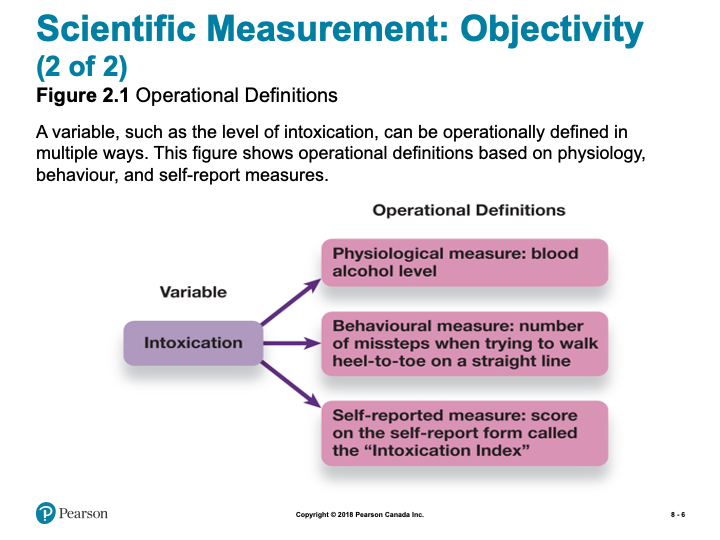
\includegraphics{assets/unit_1/PSYC106-Chs2-ResearchandThoughtandLanguage-3rdEd.png}

\emph{slide showing Operational Definitions}

Scientific Measurement: Reliability and Validity

\begin{itemize}
\tightlist
\item
  Reliability (p.~32)

  \begin{itemize}
  \tightlist
  \item
    Consistent and stable\\
  \end{itemize}
\item
  Validity (p.~32)

  \begin{itemize}
  \tightlist
  \item
    True measurements
  \end{itemize}
\end{itemize}

Generalizability of Results

\begin{itemize}
\tightlist
\item
  Generalizability (p.~33)

  \begin{itemize}
  \tightlist
  \item
    Outside the laboratory\\
  \end{itemize}
\item
  Study large groups

  \begin{itemize}
  \tightlist
  \item
    Population (p.~33)

    \begin{itemize}
    \tightlist
    \item
      Sample (p.~33)\\
    \end{itemize}
  \end{itemize}
\item
  Best reflection of population

  \begin{itemize}
  \tightlist
  \item
    Random sample (p.~33)\\
  \end{itemize}
\item
  Settle for easier sample

  \begin{itemize}
  \tightlist
  \item
    Convenience sample (p.~33)\\
  \end{itemize}
\item
  Location of study

  \begin{itemize}
  \tightlist
  \item
    Laboratory research\\
  \item
    Naturalistic research\\
  \item
    Ecological validity (p.~33)
  \end{itemize}
\end{itemize}

Sources of Bias in Psychological

\begin{itemize}
\tightlist
\item
  Research\\
\item
  Researcher Bias\\
\item
  Subject/Participant Bias\\
\item
  Hawthorne effect (p.~35)\\
\item
  Social Desirability (p.~35)
\end{itemize}

Working the Scientific Literacy Model: Demand Characteristics and
Participant Behaviour

\begin{itemize}
\tightlist
\item
  What do we know about how bias affects research participants?

  \begin{itemize}
  \tightlist
  \item
    Demand characteristics (p.~36)\\
  \end{itemize}
\item
  How can science test the effects of demand characteristics on behaviour?

  \begin{itemize}
  \tightlist
  \item
    Backpack scenario\\
  \end{itemize}
\item
  How can we critically evaluate the issue of bias in research?

  \begin{itemize}
  \tightlist
  \item
    Researcher bias

    \begin{itemize}
    \tightlist
    \item
      Bright rats vs.~dull rats\\
    \end{itemize}
  \end{itemize}
\item
  Why is this relevant?

  \begin{itemize}
  \tightlist
  \item
    Bias compromises studies\\
  \item
    Placebo effect (p.~35)
  \end{itemize}
\end{itemize}

Psych @ The Hospital: The Placebo Effect

\begin{itemize}
\tightlist
\item
  Debate about placebo effect

  \begin{itemize}
  \tightlist
  \item
    ``All in their head''\\
  \item
    Actual physiological response\\
  \end{itemize}
\item
  Brain activity in regions involved in pain

  \begin{itemize}
  \tightlist
  \item
    Multiple ways for placebos to affect our responses to pain
  \end{itemize}
\end{itemize}

Techniques That Reduce Bias

\begin{itemize}
\tightlist
\item
  Anonymity\\
\item
  Confidentiality\\
\item
  Inform participants\\
\item
  Single-blind study (p.~37)\\
\item
  Double-blind study (p.~37)
\end{itemize}

Sharing the Results

\begin{itemize}
\tightlist
\item
  Academic journals

  \begin{itemize}
  \tightlist
  \item
    Peer review (p.~37)\\
  \item
    Replication (p.~38)
  \end{itemize}
\end{itemize}

Five Characteristics of Poor Research

\begin{itemize}
\tightlist
\item
  Lack of falsifiable hypotheses (p.~38)

  \begin{itemize}
  \tightlist
  \item
    Testability requires faisifiability\\
  \end{itemize}
\item
  Anecdotal evidence (p.~38)

  \begin{itemize}
  \tightlist
  \item
    weight loss commercials\\
  \end{itemize}
\item
  Biased selection of data\\
\item
  Appeal to authority (p.~39)

  \begin{itemize}
  \tightlist
  \item
    Corresponding data?\\
  \item
    Biased expert?\\
  \end{itemize}
\item
  Appeal to common sense (p.~39)

  \begin{itemize}
  \tightlist
  \item
    Earth is centre of universe
  \end{itemize}
\end{itemize}

2.2 Learning Objectives

\begin{itemize}
\tightlist
\item
  Know the key terminology related to research designs.\\
\item
  Understand what it means when variables are positively or negatively correlated.\\
\item
  Understand how experiments help demonstrate cause-and-effect relationships.\\
\item
  Apply the terms and concepts of experimental methods to research examples.\\
\item
  Analyze the pros and cons of descriptive, correlational, and experimental research designs.
\end{itemize}

Descriptive Research

\begin{itemize}
\tightlist
\item
  Descriptive data

  \begin{itemize}
  \tightlist
  \item
    From observations\\
  \item
    No attempt to explain why\\
  \end{itemize}
\item
  Qualitative Research (p.~42)\\
\item
  Case study (p.~42)

  \begin{itemize}
  \tightlist
  \item
    Extensive details\\
  \item
    Lacks generalizability\\
  \end{itemize}
\item
  Naturalistic observation (p.~44)\\
\item
  Self-reporting (p.~45)

  \begin{itemize}
  \tightlist
  \item
    Participant makes the observations
  \end{itemize}
\end{itemize}

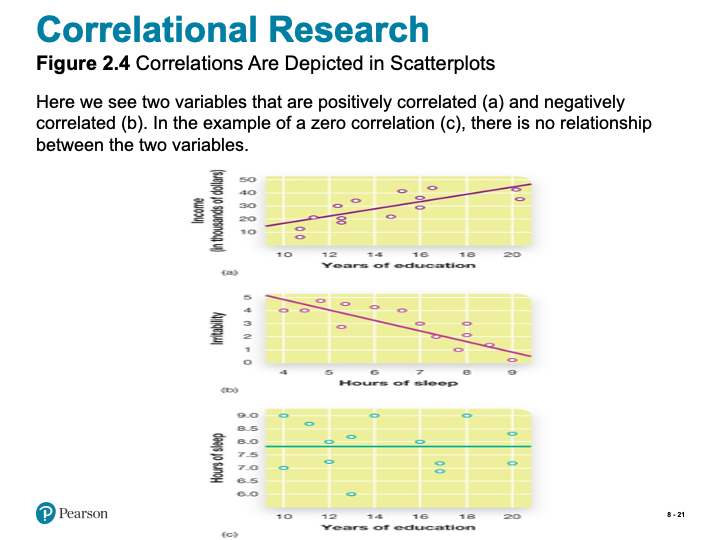
\includegraphics{assets/unit_1/slide_21.png}

\emph{Slide showing correlations depicted in scatterplots}

Myths in Mind: Beware of Illusory Correlations

\begin{itemize}
\tightlist
\item
  Illusory correlations (p.~47)

  \begin{itemize}
  \tightlist
  \item
    Crime increases when the moon is full\\
  \item
    Opposites attract\\
  \item
    Gamblers on a ``hot streak''\\
  \item
    Stereotypes
  \end{itemize}
\end{itemize}

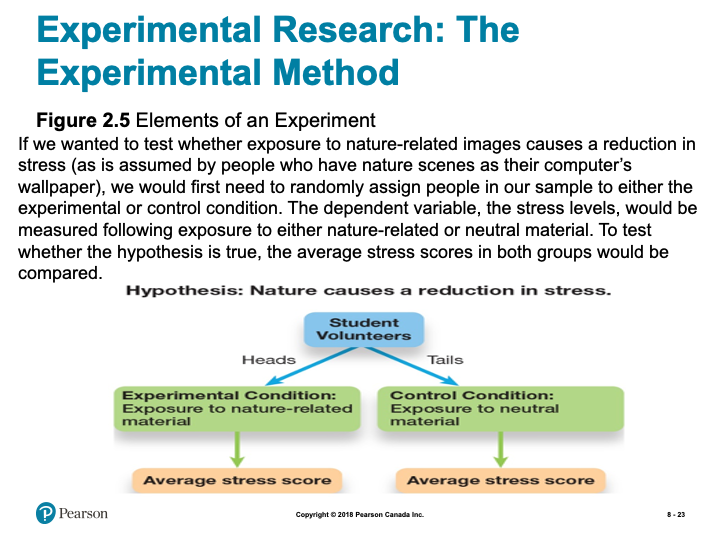
\includegraphics{assets/unit_1/slide_23.png}

\emph{Slide showing - Elements of an Experiment}

Experimental Research: The Quasi-Experimental Method

\begin{itemize}
\tightlist
\item
  Quasi-experimental research (p.~49)

  \begin{itemize}
  \tightlist
  \item
    Random assignment not always possible

    \begin{itemize}
    \tightlist
    \item
      Comparing men and women\\
    \end{itemize}
  \item
    Cannot determine cause-and-effect
  \end{itemize}
\end{itemize}

2.4 Learning Objectives

\begin{itemize}
\tightlist
\item
  Know the key terminology of statistics.\\
\item
  Understand how and why psychologists use significance tests.\\
\item
  Apply your knowledge to interpret the most frequently used types of graphs.\\
\item
  Analyze the choice of central tendency statistics based on the shape of the distribution.
\end{itemize}

Descriptive Statistics

\begin{itemize}
\tightlist
\item
  Descriptive statistics (p.~60)

  \begin{itemize}
  \tightlist
  \item
    Frequency\\
  \item
    Central tendency\\
  \item
    Variability
  \end{itemize}
\end{itemize}

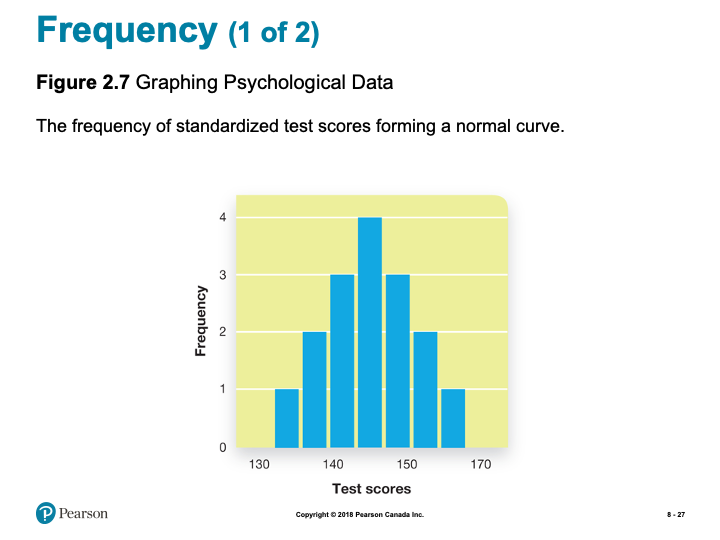
\includegraphics{assets/unit_1/slide_27.png}

\emph{Slide showing - Graphing Psychological Data}

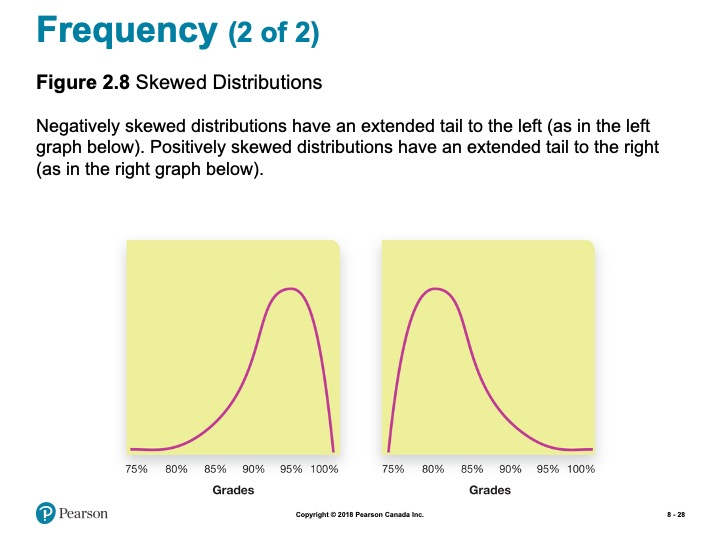
\includegraphics{assets/unit_1/slide_28.jpg}

\emph{Slide showing - Skewed Distributions}

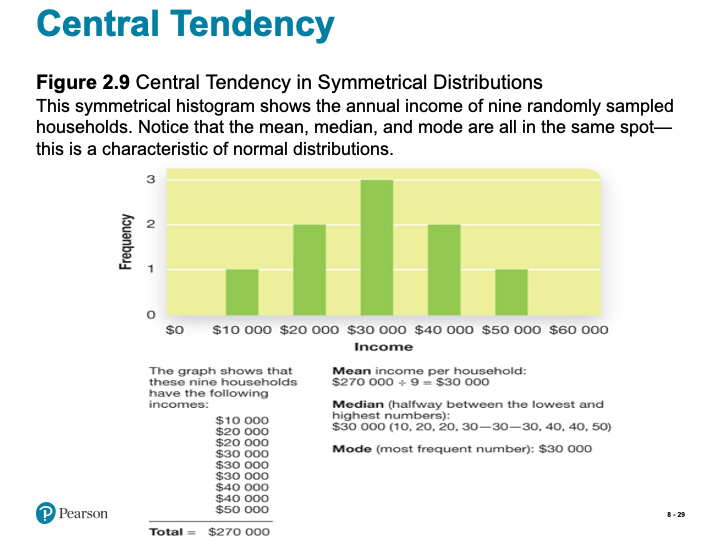
\includegraphics{assets/unit_1/slide_29.png}

\emph{Slide showing - Central Tendency in Symmetrical Distributions}

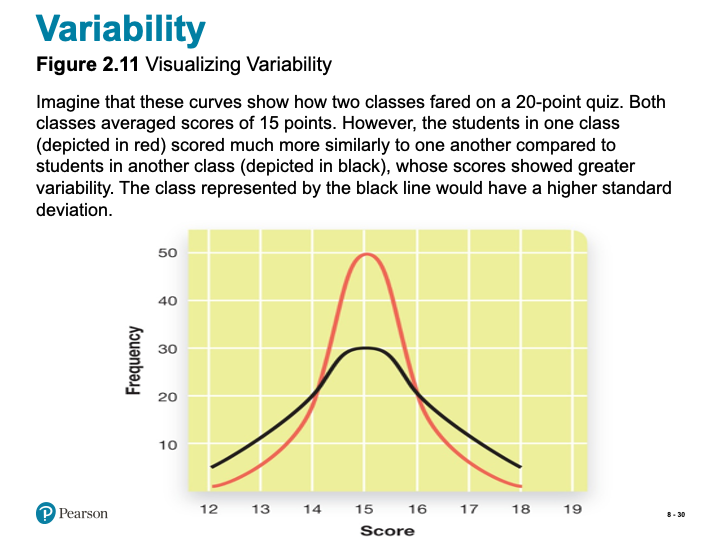
\includegraphics{assets/unit_1/slide_30.png}

\emph{Slide showing - Visualizing Variability}

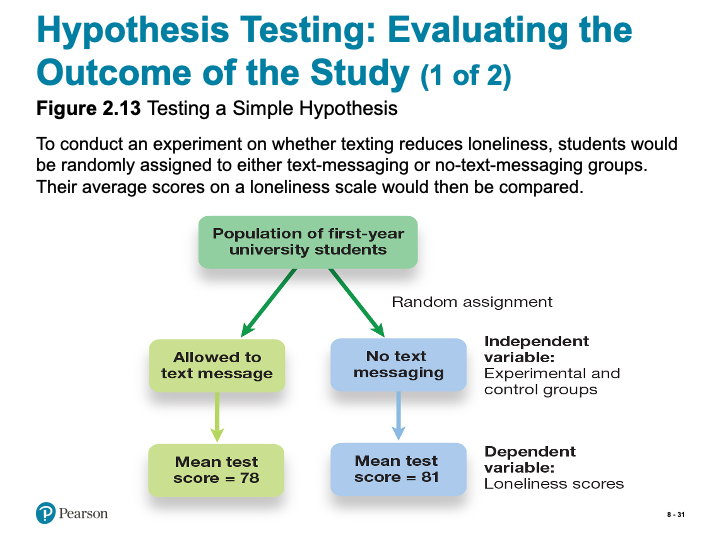
\includegraphics{assets/unit_1/slide_31.png}

\emph{Slide showing - Testing a Simple Hypothesis}

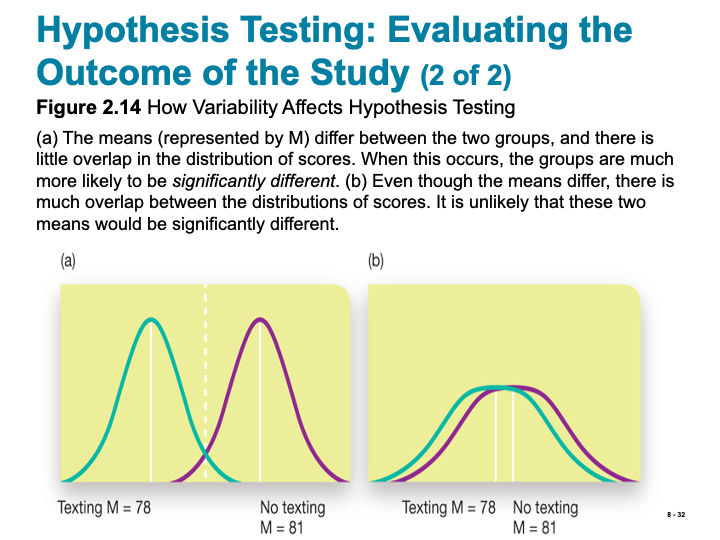
\includegraphics{assets/unit_1/slide_32.png}

\emph{Slide showing - How Variability Affects Hypothesis Testing}

True or False?

\begin{itemize}
\tightlist
\item
  T F 1. People more easily detect male prejudice against females than female against males or female against females.\\
\item
  T F 2. In general, people underestimate how much they really know.\\
\item
  T F 3. It takes less compelling evidence to change our beliefs than it did to create them in the first place.\\
\item
  T F 4. The babbling of an infant at 4 months of age makes it clear whether the infant is French, Korean, or Ethiopian.\\
\item
  T F 5. Some people can write but not read.\\
\item
  T F 6. Many bilinguals report that they have different senses of self, depending on which language they are using.\\
\item
  T F 7. Imagining a physical activity triggers action in the same brain areas that are triggered when actually performing that activity.\\
\item
  T F 8. Only human beings seem capable of insight (the sudden realization of a problem's solution).\\
\item
  T F 9. Honeybees do a dance to communicate the direction and distance of a new food source to other bees.\\
\item
  T F 10. Apes are capable of communicating meaning by using symbols.
\end{itemize}

Thinking

\begin{itemize}
\tightlist
\item
  Thinking, or \emph{cognition}, refers to a process that involves knowing, understanding, remembering, and communicating.\\
\item
  Gr. \(\Phi\rho\omega\nu\epsilon\omega\) (pr. phrones) - to think, to mind; to be of opinion; to take thought, be considerate; to entertain sentiments or inclinations of a specific kind, to be minded; to be in a certain frame of mind; to imagine; to heed, pay regard to; to incline to; be set upon, mind
\end{itemize}

A little more Greek

\begin{itemize}
\tightlist
\item
  Mind Gr. \(\Nu\omicron\upsilon\varsigma\) - the mind, intellect; understanding, intelligent faculty; intellect, judgment; opinion, sentiment; mind, thought, conception; settled state of mind; frame of mind.
\end{itemize}

The limits of intuition

\begin{itemize}
\tightlist
\item
  A bat and a ball cost \$1.10 in total. The bat costs \$1 more than the ball. How much does the ball cost?\\
\item
  A man bought a horse for \$60 and sold it for \$70. Then he bought the same horse back for \$80 and again sold it, for \$90. How much money did he make in the horse business?
\end{itemize}

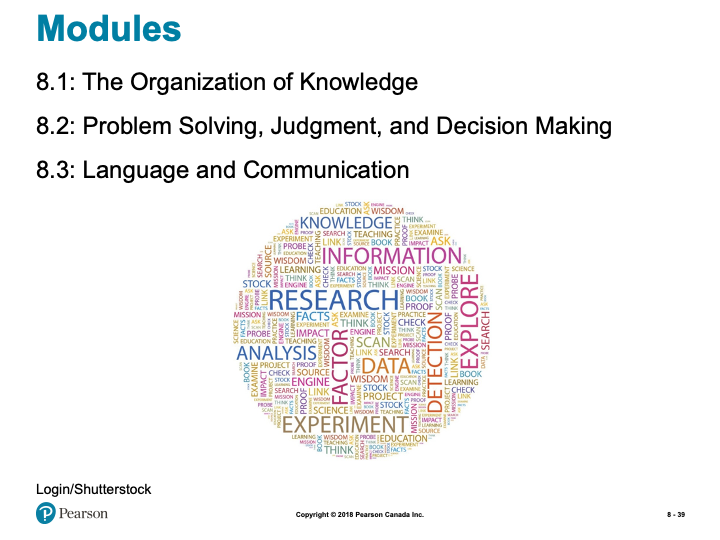
\includegraphics{assets/unit_1/slide_39.png}

\emph{Slide showing - Modules}

8.1 Learning Objectives

\begin{itemize}
\tightlist
\item
  Know the key terminology associated with concepts and categories.\\
\item
  Understand theories of how people organize their knowledge about the world.\\
\item
  Understand how experience and culture can shape the way we organize our knowledge.\\
\item
  Apply your knowledge to identify prototypical examples.\\
\item
  Analyze the claim that the language we speak determines how we think.
\end{itemize}

Concepts and Categories

\begin{itemize}
\tightlist
\item
  Concept (p.~294)

  \begin{itemize}
  \tightlist
  \item
    Divided into smaller groups\\
  \end{itemize}
\item
  Categories (p.~294)
\end{itemize}

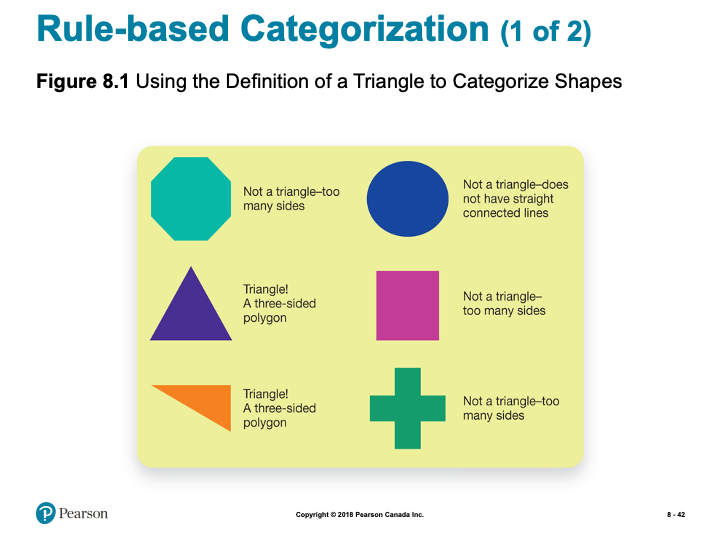
\includegraphics{assets/unit_1/slide_42.png}

\emph{Slide showing - Using the Definition of a Triangle to Categorize Shapes}

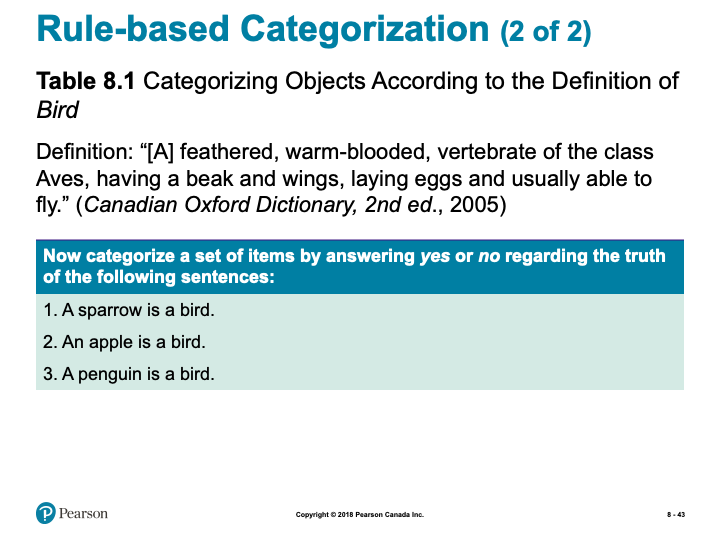
\includegraphics{assets/unit_1/slide_43.png}

\emph{Slide showing - Categorizing Objects According to the Definition of Bird}

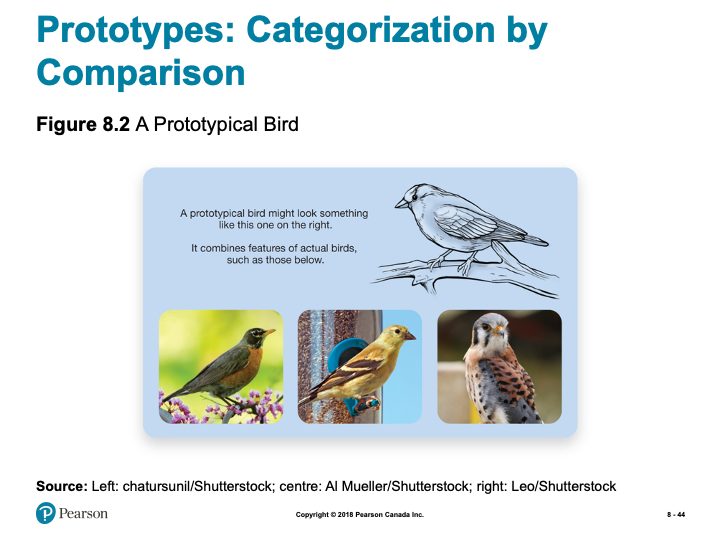
\includegraphics{assets/unit_1/slide_44.png}

\emph{Slide showing - A Prototypical Bird}

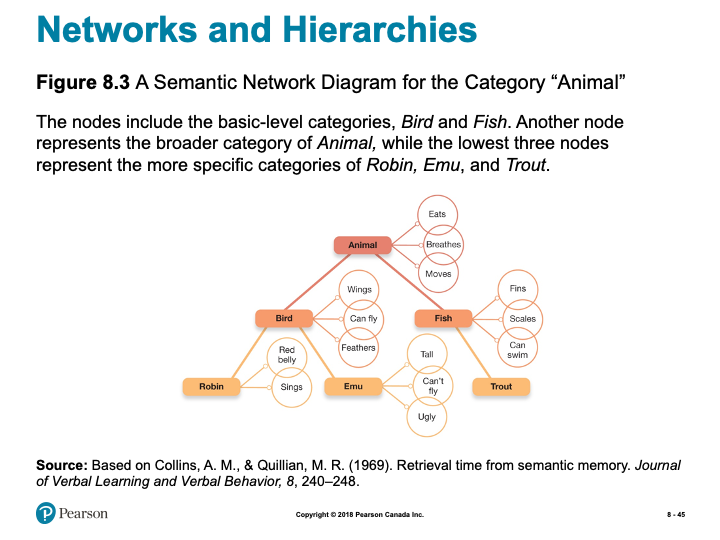
\includegraphics{assets/unit_1/slide_45.png}

\emph{Slide showing - A Semantic Network Diagram for the Category ``Animal''}

Working the Scientific Literacy Model: Priming and Semantic
Networks

\begin{itemize}
\tightlist
\item
  What do we know about semantic networks?

  \begin{itemize}
  \tightlist
  \item
    Priming (p.~297)\\
  \end{itemize}
\item
  How can scientists explain priming effects?

  \begin{itemize}
  \tightlist
  \item
    Lexical Decision Task\\
  \end{itemize}
\item
  Can we critically evaluate this information?

  \begin{itemize}
  \tightlist
  \item
    Strength of priming varies\\
  \item
    Experiments difficult to replicate\\
  \end{itemize}
\item
  Why is this relevant?

  \begin{itemize}
  \tightlist
  \item
    Advertising
  \end{itemize}
\end{itemize}

Categorization and Experience

\begin{itemize}
\tightlist
\item
  Categorization is based on experience

  \begin{itemize}
  \tightlist
  \item
    Efficient process\\
  \item
    But can also result in errors
  \end{itemize}
\end{itemize}

Categories and the Brain (1 of 2)

\begin{itemize}
\tightlist
\item
  Categories, Memories, and the Brain\\
\item
  Category-specific visual agnosia (CSVA)

  \begin{itemize}
  \tightlist
  \item
    Living vs.~non-living categories
  \end{itemize}
\end{itemize}

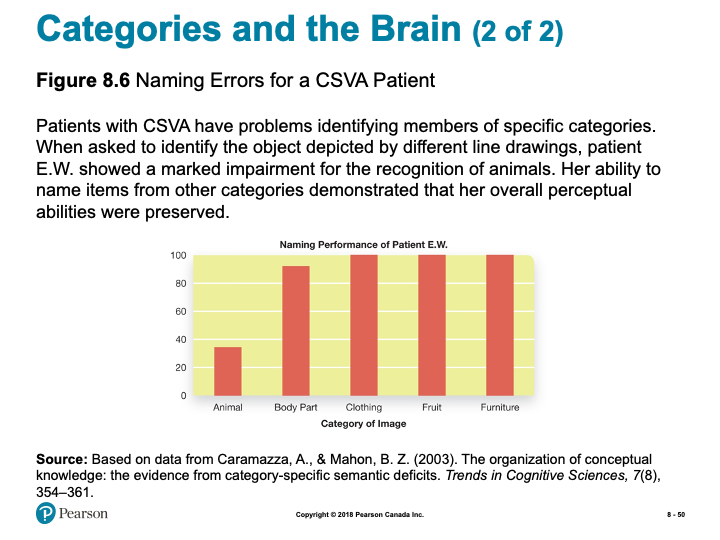
\includegraphics{assets/unit_1/slide_50.png}

\emph{Slide showing - Naming Errors for a CSVA Patient}

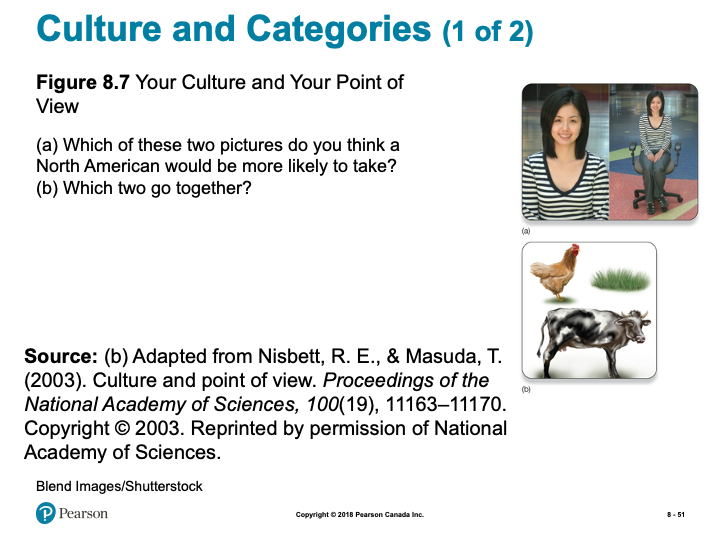
\includegraphics{assets/unit_1/slide_51.png}

\emph{Slide showing - Your Culture and Your Point of View}

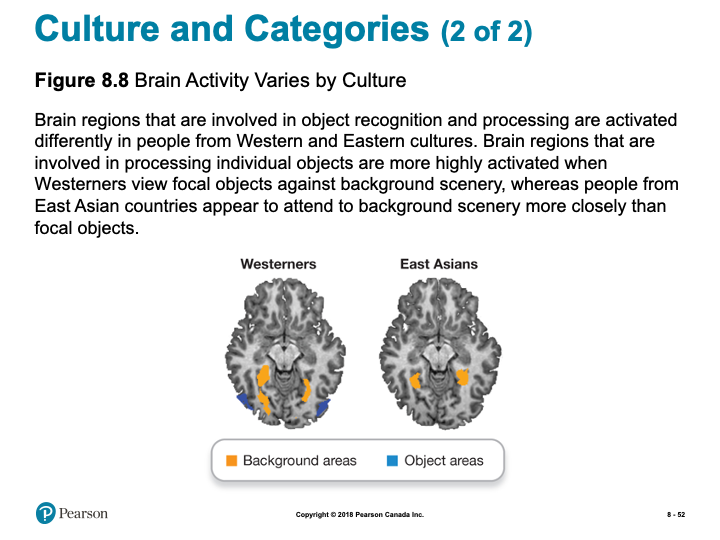
\includegraphics{assets/unit_1/slide_52.png}

\emph{Slide showing - Brain Activity Varies by Culture}

Myths in Mind: How Many Words for Snow?

\begin{itemize}
\tightlist
\item
  Inuit have many words for snow

  \begin{itemize}
  \tightlist
  \item
    Aput = snow on the ground\\
  \item
    Gana = falling snow\\
  \item
    Exaggerated to dozens of words\\
  \end{itemize}
\item
  Canadians have many words for snow

  \begin{itemize}
  \tightlist
  \item
    Sticky snow\\
  \item
    Drifting snow\\
  \item
    Yellow snow
  \end{itemize}
\end{itemize}

8.2 Learning Objectives

\begin{itemize}
\tightlist
\item
  Know the key terminology of problem solving and decision making.\\
\item
  Understand the characteristics that problems have in common.\\
\item
  Understand how obstacles to problem solving are often self-imposed.\\
\item
  Apply your knowledge to determine if you tend to be a maximizer or a satisficer.\\
\item
  Analyze whether human thought is primarily logical or intuitive.
\end{itemize}

Defining and Solving Problems

\begin{itemize}
\tightlist
\item
  Problem solving (p.~304)

  \begin{itemize}
  \tightlist
  \item
    Algorithms (p.~304)\\
  \item
    Heuristics (p.~304)
  \end{itemize}
\end{itemize}

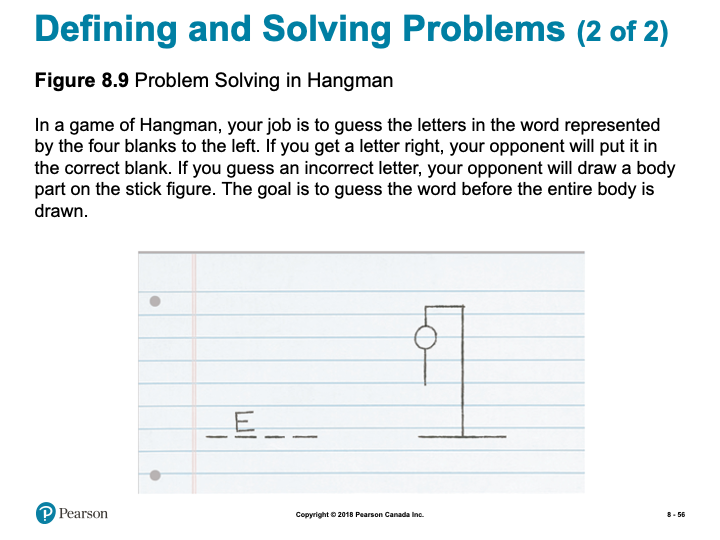
\includegraphics{assets/unit_1/slide_56.png}

\emph{Slide showing - Problem Solving in Hangman}

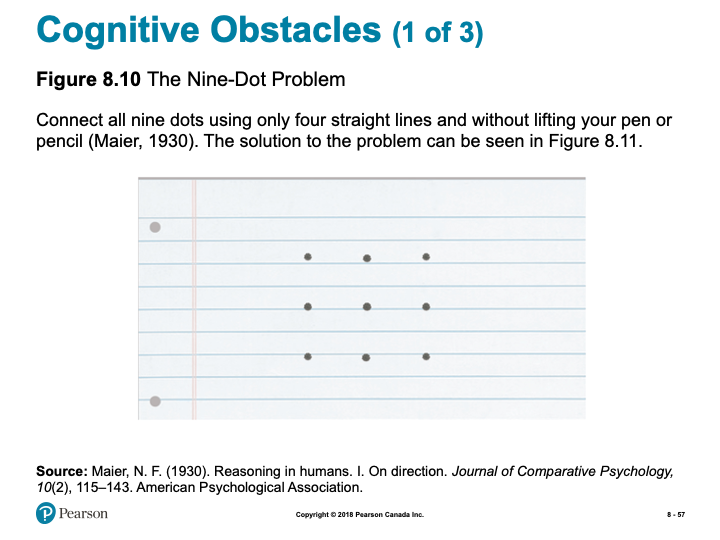
\includegraphics{assets/unit_1/slide_57.png}

\emph{Slide showing - The Nine-Dot Problem}

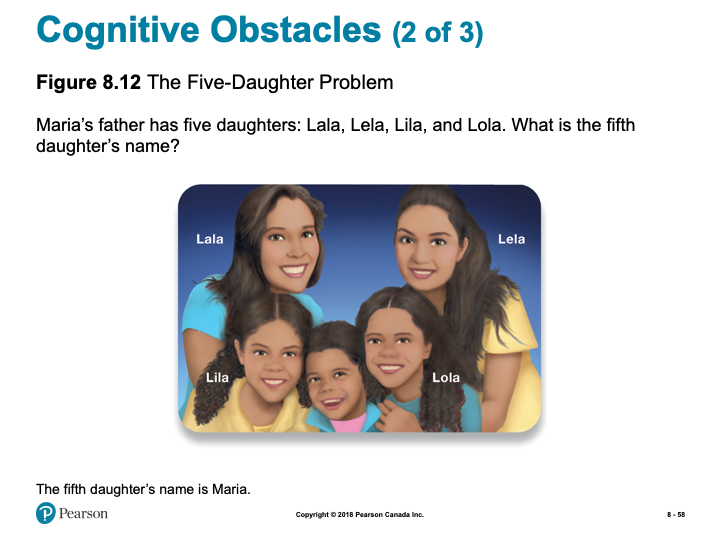
\includegraphics{assets/unit_1/slide_58.png}

\emph{Slide showing - The Five-Daughter Problem}

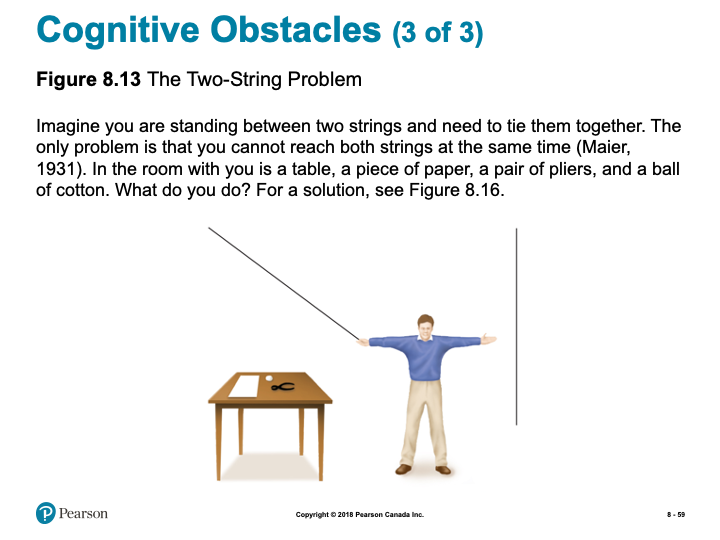
\includegraphics{assets/unit_1/slide_59.png}

\emph{Slide showing - The Two-String Problem}

Representativeness and Availability

\begin{itemize}
\tightlist
\item
  Conjunction fallacy (p.~308)\\
\item
  Representativeness heuristic (p.~308)\\
\item
  Availability heuristic (p.~308)
\end{itemize}

Anchoring Effects

\begin{itemize}
\tightlist
\item
  Anchoring effect (p.~310)

  \begin{itemize}
  \tightlist
  \item
    In what year did British Columbia become part of Canada?\\
  \item
    More affected when generated by individual
  \end{itemize}
\end{itemize}

Framing Effects

\begin{itemize}
\tightlist
\item
  Decision-making influenced by how problem is framed (p.~310)\\
\item
  Example: Vaccine A vs.~Vaccine B
\end{itemize}

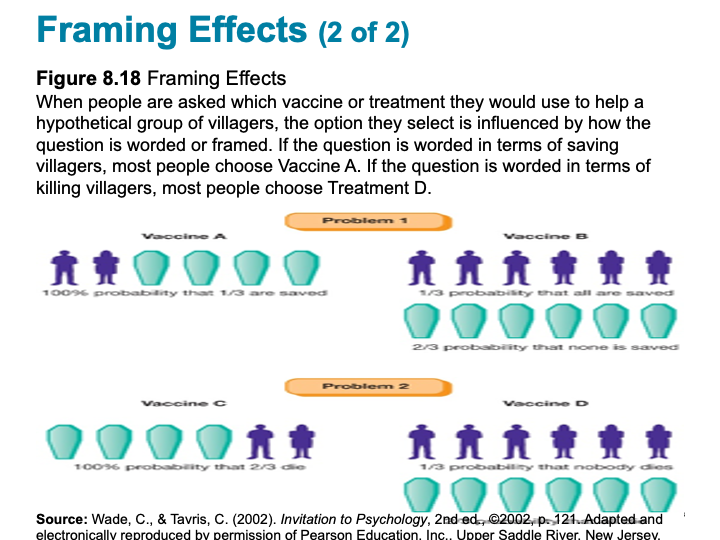
\includegraphics{assets/unit_1/slide_63.png}

\emph{Slide showing - Framing Effects}

Belief Perseverance and Confirmation Bias

\begin{itemize}
\item
  Belief perseverance (p.~310)\\
\item
  Confirmation bias (p.~311)
\item
  Can dramatically influence beliefs, especially for complex, emotionally-charged issues (e.g.~politics)
\end{itemize}

What do we know about maximizing and satisficing?

\begin{itemize}
\item
  Two types of consumers

  \begin{itemize}
  \tightlist
  \item
    Satisficers = ``good enough*\\
  \item
    Maximizers = evaluate every option\\
  \end{itemize}
\item
  Paradox of choice
\item
  How can scientists explain maximizing and satisficing?
\end{itemize}

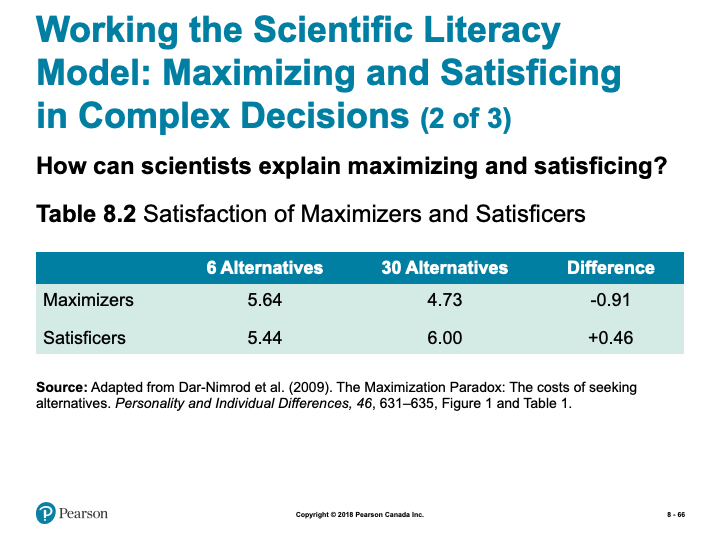
\includegraphics{assets/unit_1/slide_66.png}

\emph{Slide showing - Satisfaction of Maximizers and Satisficers}

\begin{itemize}
\tightlist
\item
  Can we critically evaluate this information?

  \begin{itemize}
  \tightlist
  \item
    Maximizers might expect more\\
  \item
    Correlational research\\
  \end{itemize}
\item
  Why is this relevant?

  \begin{itemize}
  \tightlist
  \item
    Planning for the future
  \end{itemize}
\end{itemize}

8.3 Learning Objectives

\begin{itemize}
\tightlist
\item
  Know the key terminology from the study of language.\\
\item
  Understand how language is structured.\\
\item
  Understand how genes and the brain are involved in language use.\\
\item
  Apply your knowledge to distinguish between units of language such as phonemes and morphemes.\\
\item
  Analyze whether species other than humans are able to use language.
\end{itemize}

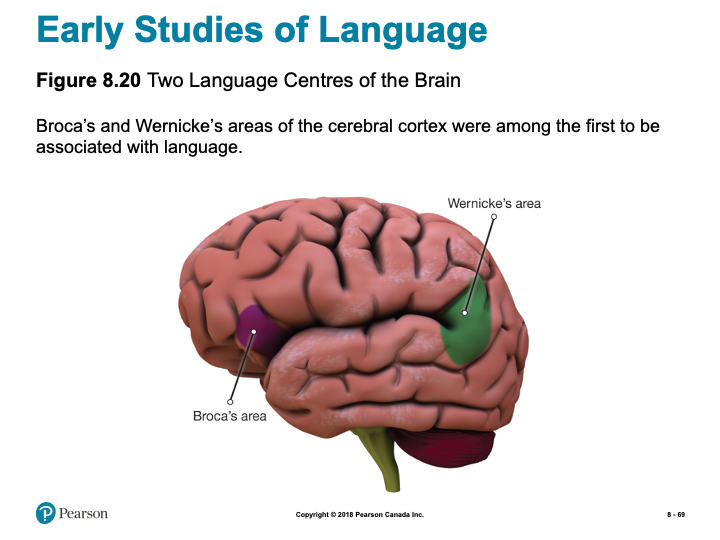
\includegraphics{assets/unit_1/slide_69.png}

\emph{Slide showing - Two Language Centres of the Brain}

Properties of Language

\begin{itemize}
\tightlist
\item
  Language (p.~317)\\
\item
  Unique features

  \begin{itemize}
  \tightlist
  \item
    Communicate objects and events not in present time and place\\
  \item
    Produce new meanings\\
  \item
    Passed down naturally to children
  \end{itemize}
\end{itemize}

Phonemes and Morphemes: The Basic Ingredients of Language

\begin{itemize}
\tightlist
\item
  Phonemes (p.~318)

  \begin{itemize}
  \tightlist
  \item
    ``T''
  \end{itemize}
\item
  Morphemes (p.~318)

  \begin{itemize}
  \tightlist
  \item
    Pig, ish, or pigish\\
  \item
    Productivity\\
  \end{itemize}
\item
  Semantics (p.~318)
\end{itemize}

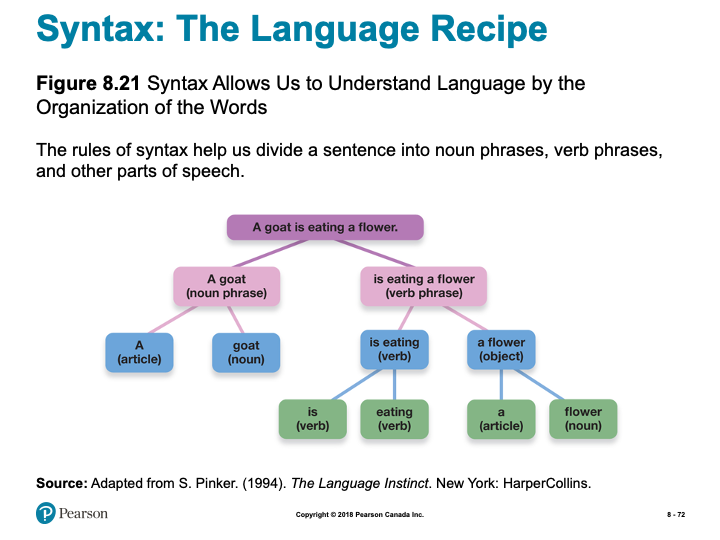
\includegraphics{assets/unit_1/slide_72.png}

\emph{Slide showing - How syntax helps us to understand language}

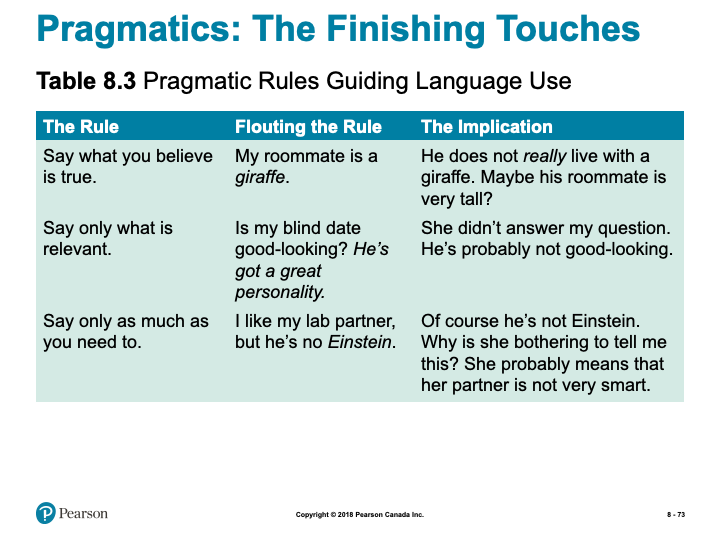
\includegraphics{assets/unit_1/slide_73.png}

\emph{Slide showing - Pragmatic Rules Guiding Language Use}

The Development of Language

-Infants, sound perception, and language acquisition
- Identifying Sounds\\
- Fast mapping (p.~320)

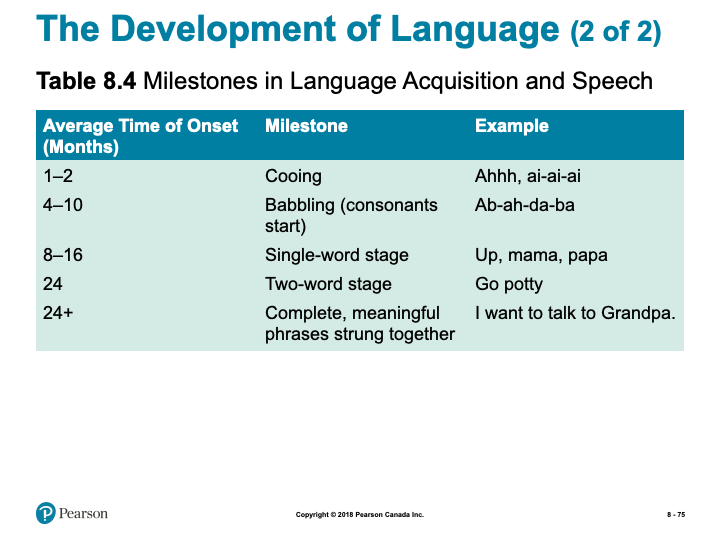
\includegraphics{assets/unit_1/slide_75.png}

\emph{Slide showing - Milestones in Language Acquisition and Speech}

Sensitive Periods for Language

\begin{itemize}
\tightlist
\item
  Sensitive period

  \begin{itemize}
  \tightlist
  \item
    Brains are primed to develop language skills\\
  \item
    Ability fades starting seventh year\\
  \item
    Same with sign language
  \end{itemize}
\end{itemize}

The Bilingual Brain

\begin{itemize}
\tightlist
\item
  Costs

  \begin{itemize}
  \tightlist
  \item
    Smaller vocabulary\\
  \item
    Word access
  \end{itemize}
\item
  Benefits

  \begin{itemize}
  \tightlist
  \item
    Executive functions\\
  \item
    Health benefits
  \end{itemize}
\end{itemize}

Working the Scientific Literacy Model: Genes and Language

\begin{itemize}
\tightlist
\item
  What do we know about genes and language?

  \begin{itemize}
  \tightlist
  \item
    Language evolved to solve problems\\
  \item
    Number of genes involved
  \end{itemize}
\item
  Which scientific evidence supports a genetic basis of language?

  \begin{itemize}
  \tightlist
  \item
    FOXP2 gene
  \end{itemize}
\end{itemize}

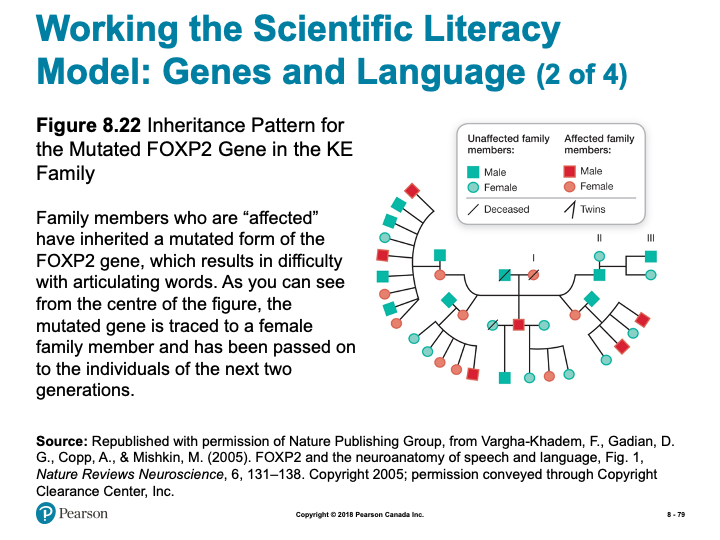
\includegraphics{assets/unit_1/slide_79.png}

\emph{Slide showing - Inheritance Pattern for the Mutated FOXP2 Gene in the KE Family}

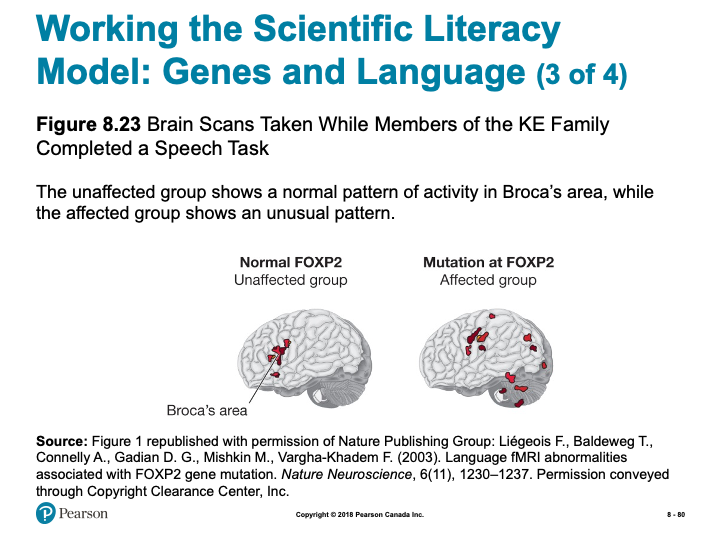
\includegraphics{assets/unit_1/slide_80.png}

\emph{Slide showing - Brain Scans Taken While Members of the KE Family Completed a Speech Task}

\begin{itemize}
\tightlist
\item
  Can we critically evaluate this evidence?

  \begin{itemize}
  \tightlist
  \item
    Many genes work together\\
  \item
    FOXP2 not unique to humans

    \begin{itemize}
    \tightlist
    \item
      Language is unique to humans
    \end{itemize}
  \end{itemize}
\item
  Why is this relevant?

  \begin{itemize}
  \tightlist
  \item
    Links between genes and language
  \end{itemize}
\end{itemize}

Can Animals Use Language?

\begin{itemize}
\tightlist
\item
  Chimpanzee Viki

  \begin{itemize}
  \tightlist
  \item
    Cross-fostered (p.~324)\\
  \item
    Four words
  \end{itemize}
\item
  Chimpanzee Washoe

  \begin{itemize}
  \tightlist
  \item
    ASL

    \begin{itemize}
    \tightlist
    \item
      200 signs\\
    \item
      Generalized words
    \end{itemize}
  \end{itemize}
\item
  Bonobo Kanzi

  \begin{itemize}
  \tightlist
  \item
    Lexigrams

    \begin{itemize}
    \tightlist
    \item
      350 symbols\\
    \item
      3,000 spoken words
    \end{itemize}
  \end{itemize}
\end{itemize}

\textbf{Note:} the slides are intended to supplement the information found in your textbook. If you are having trouble viewing them, they can also be downloaded by scrolling to the bottom of the screen and clicking on the ``Unit 1- Slides'' link.*
\end{reflect}

\hypertarget{learning-activities}{%
\subsection*{Learning Activities:}\label{learning-activities}}
\addcontentsline{toc}{subsection}{Learning Activities:}

\begin{reflect}
{Chapter 2 Review Quiz}

\begin{itemize}
\tightlist
\item
  Practice Quiz to self-assess your own comprehension of important terms from Chapter 2.\\
\item
  Not for formal evaluation.
\end{itemize}

\textbf{Problem Solving Activity}

\begin{itemize}
\tightlist
\item
  Solve some problems by utilizing some of the cognitive strategies we learned about in this topic.
\end{itemize}

{Problem Solving Practice}

\begin{itemize}
\tightlist
\item
  Explore problem solving activities and reflect on the strategies you incorporate as you discover solutions.
\end{itemize}

{Introduction to Visualizatione}

\begin{itemize}
\tightlist
\item
  Article introduces visualization and provides an opportunity to practice this skill.
\end{itemize}

{Learning Lab Preparatione}

\begin{itemize}
\tightlist
\item
  Each topic will provide a question or scenario for you to consider prior to attending your Learning Lab. Be sure to carefully consider each prompt as you will be expected to contribute to the group discussion.
\end{itemize}
\end{reflect}

\hypertarget{resources}{%
\subsection*{Resources}\label{resources}}
\addcontentsline{toc}{subsection}{Resources}

Here are some additional resources that will help you complete this unit:

\begin{itemize}
\tightlist
\item
  Krause, M., Corts, D., Smith, S. C., \& Dolderman, D. (2018). \emph{Revel for An Introduction to Psychological Science, 2nd Canadian Edition.} Pearson Ed.\\
\item
  Other resources will be provided online.
\end{itemize}

\hypertarget{what-is-psychology}{%
\section{What is Psychology}\label{what-is-psychology}}

We begin our course with a quick challenge: \textbf{\emph{In your own words, define ``psychology.''}}

According to your definition, how is psychology different from other academic areas that would study humans (\emph{for example, philosophy, literature, or history})? If you said ``Pyschology is different because it uses the scientific method''- give yourself a pat on the back

You will begin your study of the scientific method by reading your textbook. The parable below (\emph{from Philipchalk's Social Psychology textbook}), however, helps illustrate the scientific method with three ``helpful'' approaches to a problem, including a simple experiment:

\emph{Once upon a time there were three brothers. One day while they were working in their father's field, they saw an old man coming along the road. The old man greeted them, and then struggled on along the road, limping terribly. After that, every day at the same time, the brothers greeted the old man and watched as he hobbled by. When a month had passed, they were so impressed that they each did something. The first brother wrote a compelling story about perseverance in the face of the ravages of old age. It encouraged many people. The second brother painted a moving portrait of the old man, stooped over and limping along. People were inspired. The third brother, who had observed the old man very closely, asked him one day if he could exchange shoes with him. The old man was surprised, but he gladly agreed. When the old man walked away he did not limp. The next day the third brother gave the old man his shoes back and watched as he limped on his way. On the third day, the brother again exchanged shoes with the old man. Then he took the old man's shoes to a shoemaker and had them repaired. When the brother gave them back to the old man he was delighted. The old man put on the shoes, thanked the brother, and walked away without a limp.}

Although each brother made a positive contribution, the third brother solved the man's problem because he discovered its cause. To do this, \textbf{\emph{he used the scientific method and he conducted an experiment (Philipchalk, 1994).}}

I think psychology is one of the most interesting areas of study there is, first, because it studies people, people like you and me, and we're interesting Second, I like psychology because it is so broad. Psychologists, as you will soon see, study everything from nerve conduction in single cells, all the way to the influence of groups on our behaviour---and everything in between. Finally, psychologists don't just speculate and theorize, they look for evidence for their ideas. If they don't find sufficient evidence, they change their ideas; and I like that. Which leads us back to the scientific method and how psychology began.

\hypertarget{learning-activity}{%
\subsection*{Learning Activity}\label{learning-activity}}
\addcontentsline{toc}{subsection}{Learning Activity}

\begin{reflect}
{Chapter 2 Review Quiz}

In order to review some of the major concepts from the text, take the following unmarked quiz. Although you will not be evaluated on these terms, they will assist you in the assignments for this course.
\end{reflect}

\hypertarget{thinking-and-problem-solving}{%
\section{Thinking and Problem Solving}\label{thinking-and-problem-solving}}

\hypertarget{thinking}{%
\subsection*{Thinking}\label{thinking}}
\addcontentsline{toc}{subsection}{Thinking}

``So God created man in his own image, in the image of God created he him; male and female created he them.'' (Genesis 1:27)

``I will praise thee; for I am fearfully and wonderfully made.'' (Psalm 139:14)

The human image of God means many things. It seems that one aspect of this image is our thinking ability, including our ability to solve problems and speak. How important is our thinking ability in our reflection of God's image? What does your answer mean for people with less ability? What about people who lose abilities due to accident or disease (e.g., Alzheimer's patients)?

\hypertarget{algorithms-heuristics}{%
\subsection*{Algorithms \& Heuristics}\label{algorithms-heuristics}}
\addcontentsline{toc}{subsection}{Algorithms \& Heuristics}

Algorithms and heuristics can be confusing. An algorithm is a guaranteed route to a solution, but it may be the long way around to success. If you knew a person lived somewhere in a large residence hall, an algorithm for finding that individual would be to knock on every door until you located the person. Heuristics, on the other hand, sug­gest that you would first ask friends where to locate the person, or check a list, then knock on the appropriate door to locate the person. Another way to think of heuristics is the phrase ``rule of thumb.'' Can you think of some rules of thumb that you have learned from your various job experiences? They may have to do with how long to cook a hamburger, or when to refill a machine, or how to get a date.

Consider the following example and explanation taken from Invitation to Social Psychology by Ron Philipchalk:

\emph{In the second part of the book, they tell you how to crack a safe. There are all kinds of ninny-pinny, dopey things, like ``It might be a good idea to try a date for the combination, because lots of people like to use dates.'' Or ``Think of the psychology of the owner of the safe, and what he might use for the combination.'' And ``The secretary is often worried that she might forget the combination of the safe, so she might write it down in one of the following places---along the edge of her desk drawer, on a list of names and addresses . . .'' and so on . . . .}

\emph{I also did a certain amount of systematic study. For instance, a typical combination was 69-32-21. How far off could a number be when you're opening the safe? If the number was 69, would 68 work? Would 67 work? On the particular locks we had, the answer was yes for both, but 66 wouldn't work. You could be off by two in either direction. That meant you only had to try one out of five numbers, so you could try zero, five, ten, fifteen, and so on. With twenty such numbers on a wheel of 100, that was 8000 possibilities instead of the 1,000,000 you would get if you had to try every single number. . . .}

\emph{I practiced all the time on my own safe so I could do this process as fast as I could and not get lost in my mind as to which number I was pushing and mess up the first number. Like a guy who practices sleight of hand, I got it down to an absolute rhythm so I could try the 400 possible back numbers in less than half an hour. That meant I could open a safe in a maximum of eight hours---with an average time of four hours. (Surely You're Joking Mr.~Feynman, p.~140)}

Mr.~Feynman's safecracking system succeeds because he methodically works through every possible combination. By logical analysis he has discovered which 8,000 possibilities out of 1,000,000 he needs to try. We call this type of logical step-by-step procedure for solving problems an algorithm (Newell \& Simon, 1972; Simon, 1981). If you use the correct algorithm your success is guaranteed.

But sometimes it can take a long time to discover the correct algorithm. And employing an algorithm is often time consuming. Mr.~Feynman spent days developing his system and it took hours to open a safe. You could certainly open a safe much faster if you found the combination on the edge of the secretary's drawer.

The shortcuts Mr.~Feynman calls ``ninny-pinny, dopey things'' are examples of heuristics. Heuristics are rule-of-thumb strategies for solving problems, shortcuts we develop from our experience. Heuristics often help us eliminate improbable alternatives and guide us to the most likely solution to a problem. Despite his appreciation for algorithms, Mr.~Feynman discovered heuristics can be useful. He found, for example, that safe owners often did not bother to change the factory set combination when they received a new safe. In one office building the temporary factory combinations 25-0-25 or 50-25-50 opened one safe in five

Algorithms and heuristics are examples of cognitive strategies---mental plans we use to make decisions and solve problems.

\hypertarget{activity-read-and-reflect}{%
\subsection*{Activity: Read and Reflect}\label{activity-read-and-reflect}}
\addcontentsline{toc}{subsection}{Activity: Read and Reflect}

\begin{reflect}
In addition to the content above, you are also responsible for reading through the following:

\emph{Krause et. al (2018). Revel for An Introduction to Psychological Science, 2nd Canadian Edition. Chapter 8}

While all of these pages may not relate directly to this unit's discussion, consistent reading will help you keep pace, as well as provide necessary background knowledge when you need it.

{Problem Solving Activity}

In this lesson, we spent time exploring cognitive strategies used to solve problems and make decisions. We now have an opportunity to practice this on our own Take a look at the following problems and see if you can find a solution. As you work through the problems, think about what cognitive strategies you are implementing as you make each decision:

{Problem A}

\begin{itemize}
\tightlist
\item
  Take a look at the following Roman Numeral: \textbf{IX}
\item
  Now add one line to the Roman numeral \textbf{IX} to make it six
\end{itemize}

Click here for the solution.

The answer is to add a curved line shaped like an ``S'' (i.e., ``SIX''). In writing, the problem looks simple, but you might want to try it aloud on a friend. There is a mental set that one must add a straight line and have some form of Roman numeral on the page.

{Problem B}

Your task is to plant trees on Arbor Day. You have ten trees that must be planted in five rows of four trees each. How would you plant the trees?

Click here for the solution.

The answer is that you would arrange them at the vertices and cross-points of a 5-pointed star

{Problem Solving Practice}

Below is a website that provides more opportunity to work through, and solve, some problems. Specifically, this resource explores the idea of \textbf{\emph{Assumptions}} and the role assumptions play when solving problems. Furthermore, this is a valuable resource as it also explores other important techniques to be implemented when solving problems.

Click on the following link and read through the information as you continue to practice your problem solving:

\href{https://www.virtualsalt.com/crebook4.htm}{\textbf{Virtual Salt}}

{Learning Lab Preparation}

Your Learning Lab for this unit will focus on group discussion as explore the topics of this unit in more detail. As you prepare for your Learning Lab, one possible scenario that discussion will focus on is below- please prepare some thoughts to share with the group:

In the largest sense, society is breaking into two classes:

\emph{The first class are people who know how to think. These people realize that most problems are open to examination and creative solution. If a problem appears in the lives of these people, their intellectual training will quickly lead them to a solution or an alternative statement of the problem. These people are the source of the most important product in today's economy -- ideas.}

\emph{The second class, the vast majority of society, are people who cannot think for themselves. I call these people `idea consumers' -- metaphorically speaking, they wander around in a gigantic open-air mall of facts and ideas. The content of their experience is provided by television, the Internet and other shallow data pools. These people believe collecting images and facts makes them educated and competent, and all their experiences reinforce this belief. The central, organizing principle of this class is that ideas come from somewhere else, from magical persons, geniuses, `them.'}

Consider the following prompts to help better prepare for the discussion:

\begin{itemize}
\tightlist
\item
  \textbf{\emph{Do you agree or disagree with this claim?}}\\
\item
  \textbf{\emph{Do you know people that fit in the second category? What causes this difference? How might it be changed?}}
\end{itemize}
\end{reflect}

\hypertarget{cognitive-biases}{%
\section{Cognitive Biases}\label{cognitive-biases}}

As if the biases mentioned in the textbook are not enough, here are a few more to watch out for, taken from Invitation to Social Psychology by Ron Philipchalk.

\hypertarget{the-gamblers-fallacy}{%
\subsection*{The Gambler's Fallacy}\label{the-gamblers-fallacy}}
\addcontentsline{toc}{subsection}{The Gambler's Fallacy}

Jill and Bob are the parents of three boys. Jill is pregnant again, and she and Bob are hoping the baby is a girl. In fact, they are confident the baby must be a girl because their previous three children were boys. If you agree with Jill and Bob that the baby is more likely to be a girl than a boy, then you---along with Jill and Bob---may be committing the gambler's fallacy. No matter how many boys have been born, the likelihood of a girl being born is the same as it always was, approximately 50 \% (assuming no biological abnormality or medical intervention).

The gambler's fallacy arises from our failure to recognize the independence of unconnected events. The result of a coin toss does not depend on the outcome of previous tosses; a child's sex at conception is not affected by the sex of prior conceptions; the cards dealt in a hand are not influenced by the distribution of cards on the previous deal; and so on. Each event in these sequences is independent of the others, although we tend to think that somehow there must be a connection.

\hypertarget{the-anchoring-and-adjustment-heuristic}{%
\subsection*{The Anchoring and Adjustment Heuristic}\label{the-anchoring-and-adjustment-heuristic}}
\addcontentsline{toc}{subsection}{The Anchoring and Adjustment Heuristic}

First impressions of a person exert a powerful influence on the way we interpret subsequent information about that person. This effect may be an example of a more general principle called the anchoring and adjustment heuristic. Information we use to establish a starting value (or anchor point) tends to be more influential in our decisions than subsequent information we use to adjust this value (Tversky \& Kahneman, 1974).

Daniel Cervone and his colleagues found, for example, that initial success or failure on a task can establish an anchor for feelings of self-efficacy. Students who initially succeed on a task and later fail have higher feelings of self-efficacy than students who initially fail and later succeed even though their overall level of success is the same. Final judgments of self-efficacy are biased in the direction of initial judgments (Cervone \& Palmer, 1990; Peake \& Cervone, 1989).

Salespeople often use the anchoring and adjustment heuristic to their advantage. Some real estate agents routinely show their clients an over-priced and unattractive house first in order to set an anchor point which, in effect, says, ``The kind of house you want is going to cost a lot.'' Once established, this expectation of high price changes very slowly and the clients are relieved to find an acceptable house in their price range (Northcraft \& Neale, 1987).

Car dealers too like us to set our sights high. Their so-called list price establishes an anchor or reference point that overshadows our subsequent evaluations, as I recently discovered. In looking for a certain model of car, I was attracted to a particular vehicle with an asking price of \$3,800 (``reduced from \$4,200''). I believed this price was too high, so I bargained with the vendor. Eventually, I bought the car for \$2,800. Did the high original asking price affect my decision? Yes, it probably did. Subsequent events indicated I still paid too much. I later bought an identical model in only slightly poorer condition for \$2,000. I was a victim of the anchoring and adjustment heuristic.

\textbf{\emph{Contrast Effects}}

My car purchase also illustrates a related distortion in judgment, the contrast effect. In contrast to the original price of \$4,200 my offer of \$2,800 seemed like a bargain. John Lynch, Jr.~and his colleagues (1991) found a similar effect with students. The students rated low-priced cars as less expensive when they were considered alongside high-priced cars (contrast effect), compared to when they were considered along with other low-priced cars (no contrast).

Research by Douglass Kenrick and his colleagues indicates that we also show contrast effects in evaluating other people. In one study (1980), male college students rated the attractiveness of potential blind dates. Subjects who gave their ratings after watching a TV show with attractive female actresses rated the potential dates as less attractive than did subjects who rated their potential dates before watching the show. In another study (1989), after viewing centerfold erotica, men found average women---and even their own wives---less attractive.

\hypertarget{heuristics-biases}{%
\subsection*{Heuristics \& Biases}\label{heuristics-biases}}
\addcontentsline{toc}{subsection}{Heuristics \& Biases}

By now you may be wondering why we fall prey to so many cognitive biases and errors. Well don't worry; our biases are actually a side effect of our cognitive efficiency. Most of our biases result from using heuristics, rules of thumb, or mental shortcuts that work very well. Sometimes they let us down, but overall, they improve the speed with which we handle mental problems---much like Mr.~Feynman's safe-cracking tricks. As we noted in the previous discussion, you could certainly open a safe much faster if you found the combination on the edge of the secretary's drawer. However, you won't always find the combination there, so limiting yourself to this approach would produce a kind of ``cognitive bias'' in your safe-cracking strategy.

\hypertarget{resources-online-articles-of-interest}{%
\subsection*{RESOURCES: Online Articles of Interest}\label{resources-online-articles-of-interest}}
\addcontentsline{toc}{subsection}{RESOURCES: Online Articles of Interest}

For additional information and examples, click on the link below:

\href{https://en.wikipedia.org/wiki/List_of_cognitive_biases}{\textbf{Cognitive Biases}}

\hypertarget{learning-lab-preparation}{%
\subsection*{Learning Lab Preparation}\label{learning-lab-preparation}}
\addcontentsline{toc}{subsection}{Learning Lab Preparation}

Another focus of our discussion during our Learning Lab for this unit, will focus on biases. In order to prepare for participation in this discussion, consider the guiding prompt below- be sure to have some thoughts to contribute to the discussion:

\textbf{\emph{Give an example from your own experience of one of the cognitive biases, discussed here or in the textbook, that you have fallen prey to.}}

\hypertarget{language-and-thought}{%
\section{Language and Thought}\label{language-and-thought}}

\hypertarget{linguistic-relativity}{%
\subsection*{Linguistic Relativity}\label{linguistic-relativity}}
\addcontentsline{toc}{subsection}{Linguistic Relativity}

Benjamin Whorf's linguistic relativity hypothesis suggests that our language affects the way we see the world. Do you know any examples of weather terms, for example, that are unique to one area? Could knowing these terms help you to notice differences in weather that outsiders might not notice? What about in sports? Sports fans usually know terms to de­scribe certain strokes or plays. Does knowledge of these terms affect percep­tion? Can you think of some examples? What does it mean to ``clothesline'' someone, or ``post-up,'' or ``birdie?''

\hypertarget{imaginary-practice}{%
\subsection*{Imaginary Practice}\label{imaginary-practice}}
\addcontentsline{toc}{subsection}{Imaginary Practice}

Mental practice is now widely accepted in many areas. The following excerpt is taken from the \href{https://www.golfpsych.com}{\textbf{GolfPsych}} website. You may find further examples there as well.

``You can practice the mental aspects of your game anytime. We encourage our clients to do imagery practice of playing well in upcoming tournaments. This imaginary practice includes seeing the course, situation, doing a full mental pre-shot routine and seeing a good shot. You should also be feeling the way you do when you play your best. In addition, you should be practicing deep breathing and quieting your mind off-course. This is an extremely valuable tool that must be practiced to be effective. The mental game is much more than thinking positive thoughts. Take our Personality Assessment and get your own GolfPsych Report to receive our recommendations for you based on your personality and our research. Reading our book will also help you understand all aspects of a good mental game. During your practices and before your rounds you should also be practicing your mental skills.''

\hypertarget{activity-introduction-to-visualization}{%
\subsection*{Activity: Introduction to Visualization}\label{activity-introduction-to-visualization}}
\addcontentsline{toc}{subsection}{Activity: Introduction to Visualization}

\begin{reflect}
In this Topic, we learned about the notion of mental practice. Below is an article that will take you through the process of visualization. Take some time to read the article and practice for yourself. Pay careful attention to your thoughts, your focus, your feelings as you engage in the process.

\begin{itemize}
\tightlist
\item
  \href{https://www.forbes.com/sites/bhaligill/2017/06/22/new-to-visualization-here-are-5-steps-to-get-you-started/\#60dafcdc6e3f}{\textbf{Introduction to Visualization}}
\end{itemize}

{Learning Lab Preparation}

The subject of our focus for this Topic has been on the power of language in influencing how we see the world. Our discussion during Learning Lab this week will focus on the importance of language in the Bible (and other religious writings) and how it ``shapes'' how we see the world.

To prepare for this discussion, consider the following prompt:

\textbf{\emph{Give some examples of the importance of language in the Bible or other religious writings.}}
\end{reflect}

\hypertarget{animal-language}{%
\section{Animal Language}\label{animal-language}}

\hypertarget{language}{%
\subsection*{Language}\label{language}}
\addcontentsline{toc}{subsection}{Language}

As a Christian I am pleased to see in psychology the resurgence of interest in studying some of what Ronald Koteskey (1980) calls humanity's ``God-like'' characteristics, creativity, imagery, and particularly language.

The use of words is extremely important in Christian scripture. God spoke the creation into existence; Jesus is called the Word; the significance of Babel and Pentecost are closely linked to the importance of language; and there is great power associated with an individual's name. In addition, Christians have usually considered the ability to communicate with words to be part of the image of God in man. However, recently several researchers claim to have taught animals, usually chimpanzees or apes, to communicate through language. Using sign language, blocks, or keyboards and computer- generated voices, the animals have signaled their needs and even generated word combinations.

But is this truly language? There is no doubt that the animals are using symbols as signs to stand for objects and actions. However, there are significant questions being raised about the comparison with human language.

Christians need to think carefully about what they mean when they talk about the image of God in man. The area of human learning and psycholinguistics offers some intriguing questions for thoughtful Christians. What is the origin of human speech-is it learned (as Skinner would say) or largely innate (as Chomsky would say)? Is human speech unique? Do the studies of language in animals necessitate a redefinition of the uniqueness of man? (Based on Psychology and Christianity by Ron Philipchalk, p.~102)

\hypertarget{resources-online-articles-of-interest-1}{%
\subsection*{RESOURCES: Online Articles of Interest}\label{resources-online-articles-of-interest-1}}
\addcontentsline{toc}{subsection}{RESOURCES: Online Articles of Interest}

To add to our exploration of this topic, take a moment to read the following articles:

\begin{itemize}
\item
  \href{http://tuvalu.santafe.edu/~johnson/articles.chimp.html}{\textbf{Chimp Talk Debate: Is It Really Language?}}
\item
  \href{https://www.massey.ac.nz/~alock/hbook/ristau.htm}{\textbf{Animal Language and Cognition Projects}}
\end{itemize}

\hypertarget{activity-learning-lab-preparation}{%
\subsection*{Activity: Learning Lab Preparation}\label{activity-learning-lab-preparation}}
\addcontentsline{toc}{subsection}{Activity: Learning Lab Preparation}

\begin{reflect}
Finally, take a moment to consider the following questions:

\textbf{\emph{How important for our understanding of who we are as humans is the distinctiveness of our language ability? Is it a sign of the image of God?}}

Be prepared to share your thoughts during discussion at your Learning Lab.
\end{reflect}

\hypertarget{assessment}{%
\section*{Assessment}\label{assessment}}
\addcontentsline{toc}{section}{Assessment}

\begin{assessment}
While there is no ``formal'' assignment that you will be responsible for submitting for Unit 1, you will be expected to participate in discussion during your Learning Lab. Your facilitator will be providing a participation mark based on your contributions. Below is some information to consider prior to attending your Learning Lab:

\emph{Active participation in group exercises, reflection, and critical discourse is an essential component of this course. You are expected to show respect for all members of the course, both in your speech and actions. Contribute by actively observing and listening, raising thoughtful questions, examining relevant issues, building on others' ideas, analyzing and evaluating the group's thinking, synthesizing key points, and expanding the group's perspectives. Take care not to dominate a conversation, giving space for others to speak. When in small groups help maintain the focus, flow, and quality of conversations, and take the initiative to invite others (particularly those who are quiet) to speak.}

\textbf{Rubric for Participation in Learning Labs}

\begin{longtable}[]{@{}
  >{\raggedright\arraybackslash}p{(\columnwidth - 4\tabcolsep) * \real{0.3333}}
  >{\raggedright\arraybackslash}p{(\columnwidth - 4\tabcolsep) * \real{0.3333}}
  >{\raggedright\arraybackslash}p{(\columnwidth - 4\tabcolsep) * \real{0.3333}}@{}}
\toprule\noalign{}
\begin{minipage}[b]{\linewidth}\raggedright
Emerging (0-64\%)
\end{minipage} & \begin{minipage}[b]{\linewidth}\raggedright
Developing (65-89\%)
\end{minipage} & \begin{minipage}[b]{\linewidth}\raggedright
Mastering (90-100\%)
\end{minipage} \\
\midrule\noalign{}
\endhead
\bottomrule\noalign{}
\endlastfoot
Never to almost never: Demonstrates active listening (as indicated by disengaged body language and no to rare comments that build on others' remarks),Initiates any contributions in class or small groups, Makes insightful or constructive comments, Helps maintain a supportive space for others to speak. & Sometimes to fairly often: Demonstrates active listening (as indicated by somewhat to often engaged body language and comments that build on others' remarks), Initiates a contribution at least once in a class or small group discussion; Makes insightful or constructive comments, Helps maintain a supportive space for others to speak. & Very often to nearly always: Demonstrates active listening (as indicated by fully engaged body language and comments that build on others' remarks), Initiates more than one contribution in a class or small group discussion, Makes insightful or constructive comments, Creates a space for others to speak and takes initiative to include others. \\
\end{longtable}
\end{assessment}

\hypertarget{checking-your-learning}{%
\section*{Checking your Learning}\label{checking-your-learning}}
\addcontentsline{toc}{section}{Checking your Learning}

\begin{progress}
Before you move on to the next unit, check that you are able to:

\begin{itemize}
\tightlist
\item
  Define key terminology related to principles of scientific research, research designs, and statistics.\\
\item
  Explain the five characteristics of quality scientific research, and the pros and cons of descriptive, correlational, and experimental research designs.\\
\item
  Determine how biases might influence the outcome of a study and how experiments help demonstrate cause-and-effect relationships.\\
\item
  Apply the concepts of reliability and validity to examples and concepts of experimental methods to research examples.\\
\item
  Assess whether anecdotes, authority figures, and common sense are reliably truthful sources of information.\\
\item
  Understand what it means for variables to be positively or negatively correlated and how and why psychologists use significance tests.
\end{itemize}
\end{progress}

\hypertarget{intelligence-testing}{%
\chapter{Intelligence Testing}\label{intelligence-testing}}

\hypertarget{overview-1}{%
\section*{Overview}\label{overview-1}}
\addcontentsline{toc}{section}{Overview}

In this unit, you will learn about techniques and tools for measuring intelligence, different theories as to what constitutes intelligence, and the biological, environmental, and behavioural factors that influence intelligence.

\hypertarget{topics-1}{%
\subsection*{Topics}\label{topics-1}}
\addcontentsline{toc}{subsection}{Topics}

This unit is divided into the following topics:

\begin{enumerate}
\def\labelenumi{\arabic{enumi}.}
\tightlist
\item
  What is Intelligence?\\
\item
  Extremes of Intelligence\\
\item
  Nature-Nature and IQ
\end{enumerate}

\hypertarget{learning-outcomes-1}{%
\subsection*{Learning Outcomes}\label{learning-outcomes-1}}
\addcontentsline{toc}{subsection}{Learning Outcomes}

By the end of this unit, students will be able to:

\begin{itemize}
\tightlist
\item
  Know and define the key terminology associated with understanding intelligence, intelligence testing, and heredity, environment, and intelligence.\\
\item
  Understand the reasoning behind the eugenics movements and its use of intelligence tests, why intelligence is divided into fluid and crystallized types, and the genetic basis of intelligence.\\
\item
  Apply the concepts of entity theory and incremental theory to help kids succeed in school, to identify examples from the triarchic and multiple theories of intelligence, and to recognize environmental and behavioural effects on intelligence to understand how to enhance your own cognitive abilities.\\
\item
  Analyze why it is difficult to remove all cultural bias from intelligence testing and whether teachers should spend time tailoring lessons to each individual student's learning style.
\end{itemize}

\hypertarget{activity-checklist-1}{%
\subsection*{Activity Checklist}\label{activity-checklist-1}}
\addcontentsline{toc}{subsection}{Activity Checklist}

Here is a checklist of learning activities you will benefit from in completing this unit. You may find it useful for planning your work.

\begin{reflect}
{Read and Reflect}

\begin{itemize}
\tightlist
\item
  Read \emph{Krause et al.~(2021). Revel for An Introduction to Psychological Science, 3rd Canadian Edition}\\
\item
  Review \textbf{Unit 2 - Slides}
\end{itemize}

CLICK HERE

An Introduction to Psychological Science - Chapter 9:Intelligence Testing

\begin{itemize}
\tightlist
\item
  Chapter 9 -- Intelligence Testing

  \begin{itemize}
  \tightlist
  \item
    Biblical Word Study Related to Ch. 8
  \end{itemize}
\end{itemize}

Proverbs 2:6

\begin{itemize}
\item
  \textsuperscript{6} For the LORD gives wisdom, and from his mouth come knowledge and understanding.
\end{itemize}

Greek Word Study

\begin{itemize}
\tightlist
\item
  Wisdom

  \begin{itemize}
  \tightlist
  \item
    Gr. \(\Sigma\omicron\phi\iota\alpha\) (Sophia) (Noun) -- wisdom in general, knowledge; ability; practical wisdom, prudence; learning, science; scientific skill; professed wisdom, human philosophy, superior knowledge and enlightenment; in N.T. divine wisdom, Christian enlightenment\\
  \end{itemize}
\item
  Wise

  \begin{itemize}
  \tightlist
  \item
    Gr. \(\Sigma\omicron\phi\omicron\varsigma\) (Sophos) (Adjective) -- wise generally; shrewd, clever; learned, intelligent; in N.T. divinely instructed; furnished with Christian wisdom, spiritually enlightened
  \end{itemize}
\item
  Intelligence

  \begin{itemize}
  \tightlist
  \item
    Gr.\(\Sigma\upsilon\nu\eta\sigma\iota\varsigma\) (Noun) -- pr. a sending together, a junction, as of streams; met. understanding, intelligence, discernment; the understanding, intellect, mind\\
  \end{itemize}
\item
  Intelligent

  \begin{itemize}
  \tightlist
  \item
    Gr. \(\Sigma\upsilon\nu\eta\tau\omicron\sigma\) (Synetos) (Adj.) -- intelligent, discerning, wise, prudent (cautious; worldly wise; exercising sound judgment)
  \end{itemize}
\end{itemize}

The Psychology of Wisdom

\begin{itemize}
\tightlist
\item
  Difficult life dilemmas:

  \begin{itemize}
  \tightlist
  \item
    ``A 15yearold girl wants to get married right away. What should one/she do and consider?''
  \end{itemize}
\item
  Or, ``Imagine a good friend of yours calls you up and tells you that she can't go on anymore and has decided to commit suicide. What would one/you be thinking about? How would one deal with this situation?''\\
\item
  Or, ``A 60 year old widow has recently completed a college degree and opened a business, only to learn that her son has been left alone with two small children to care for. What should she do?''
\end{itemize}

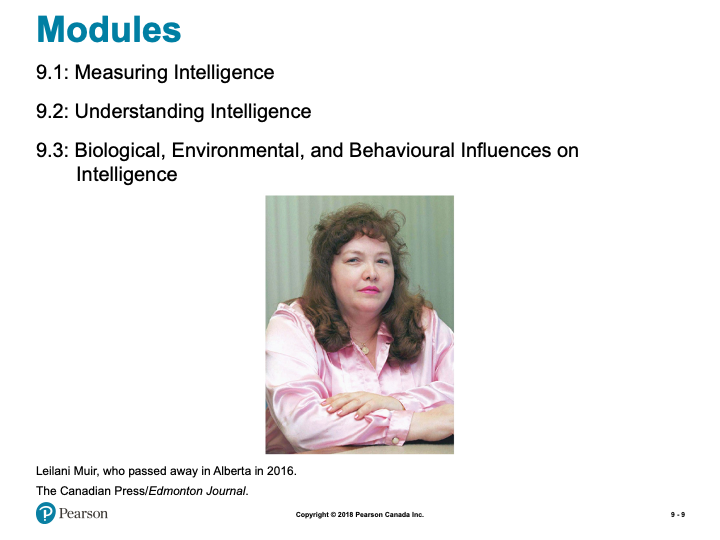
\includegraphics{assets/unit_2/slide_9.png}

\emph{Modules}

9.1 Learning Objectives

\begin{itemize}
\tightlist
\item
  Know the key terminology associated with intelligence and intelligence testing.\\
\item
  Understand the reasoning behind the eugenics movements and its use of intelligence tests.\\
\item
  Apply the concepts of entity theory and incremental theory to help kids succeed in school.\\
\item
  Analyze why it is difficult to remove all cultural bias from intelligence testing.
\end{itemize}

Different Approaches to Intelligence Testing (1 of 2)

\begin{itemize}
\tightlist
\item
  Sir Francis Galton

  \begin{itemize}
  \tightlist
  \item
    Anthropometrics (p.~329)\\
  \end{itemize}
\item
  Alfred Binet

  \begin{itemize}
  \tightlist
  \item
    Intelligence (p.~330)\\
  \item
    Mental age (p.~330)\\
  \end{itemize}
\item
  Lewis Terman

  \begin{itemize}
  \tightlist
  \item
    Stanford-Binet Test (p.~330)\\
  \end{itemize}
\item
  William Stern

  \begin{itemize}
  \tightlist
  \item
    Intelligence Quotient (IQ) (p.~330)
  \end{itemize}
\end{itemize}

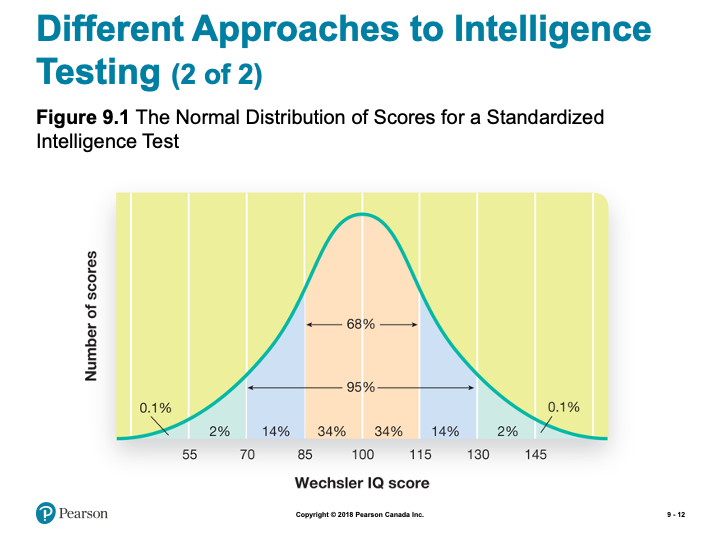
\includegraphics{assets/unit_2/slide_12.png}

\emph{Slide showing - The Normal Distribution of Scores for a Standardized Intelligence Test}

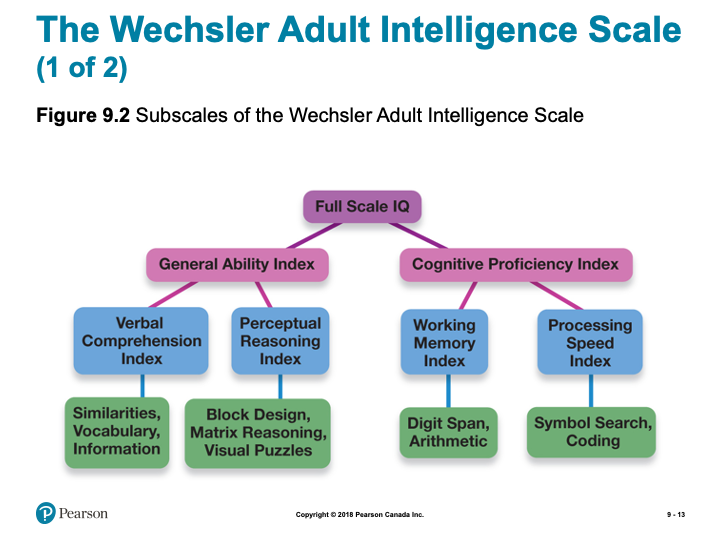
\includegraphics{assets/unit_2/slide_13.png}

\emph{Slide showing - Subscales of the Wechsler Adult Intelligence Scale}

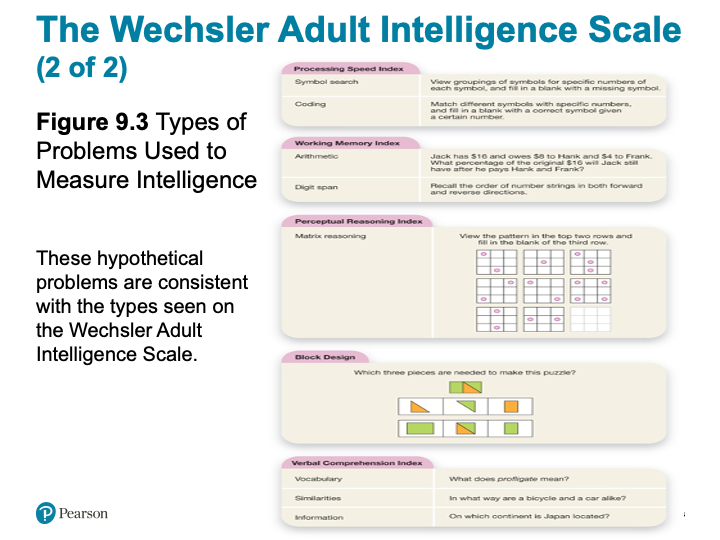
\includegraphics{assets/unit_2/slide_14.png}

\emph{Slide showing - The Wechsler Adult Intelligence Scale}

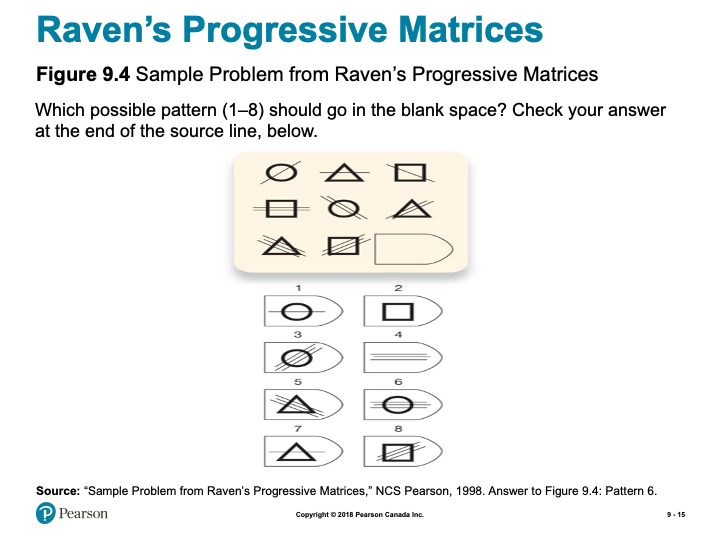
\includegraphics{assets/unit_2/slide_15.png}

\emph{Slide showing - Sample Problem from Raven's Progressive Matrices}

The Checkered Past of Intelligence Testing

\begin{itemize}
\tightlist
\item
  IQ Testing and Eugenics

  \begin{itemize}
  \tightlist
  \item
    Historical context\\
  \item
    Social Darwinism\\
  \item
    Eugenics
  \end{itemize}
\end{itemize}

The Race and IQ Controversy

\begin{itemize}
\tightlist
\item
  Racial differences in IQ scores Problems with the racial superiority interpretation

  \begin{itemize}
  \tightlist
  \item
    Culturally biased test content\\
  \item
    Culturally biased test process\\
  \item
    Stereotype threat (p.~336)
  \end{itemize}
\end{itemize}

Working the Scientific Literacy Model: Beliefs About Intelligence

\begin{itemize}
\tightlist
\item
  What do we know about the kinds of beliefs that may affect test scores?

  \begin{itemize}
  \tightlist
  \item
    Entity theory (p.~336)\\
  \item
    Incremental theory (p.~336)\\
  \end{itemize}
\item
  How can science test whether beliefs affect performance?
\end{itemize}

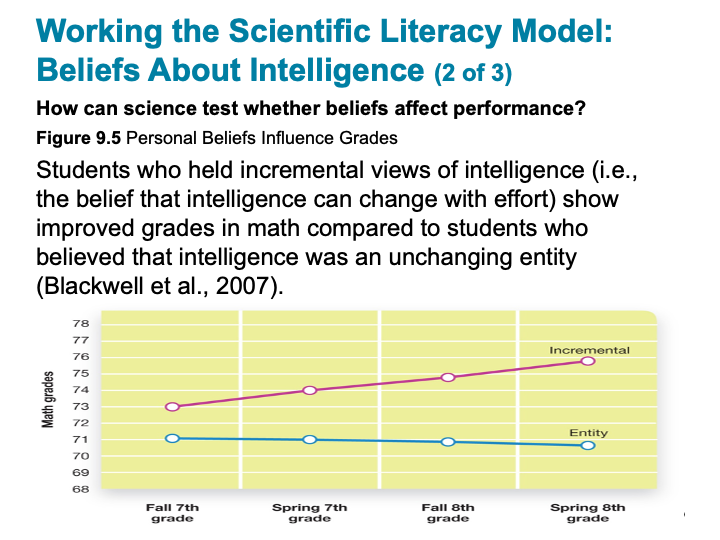
\includegraphics{assets/unit_2/slide_19.png}

\emph{Slide showing - Personal Beliefs Influence Grades}

\begin{itemize}
\tightlist
\item
  Can we critically evaluate this research?\\
\item
  Why is this relevant?
\end{itemize}

9.2 Learning Objectives

\begin{itemize}
\tightlist
\item
  Know the key terminology related to understanding intelligence.\\
\item
  Understand why intelligence is described as a hierarchy.\\
\item
  Understand intelligence differences between males and females.\\
\item
  Apply your knowledge to identify examples that reflect fluid vs.~crystallized intelligence.\\
\item
  Analyze whether teachers should spend time tailoring lessons to each individual student's learning style.
\end{itemize}

Intelligence as a Single, General Ability

\begin{itemize}
\tightlist
\item
  Spearman's general intelligence

  \begin{itemize}
  \tightlist
  \item
    General intelligence factor, ``g'' (p.~340)
  \end{itemize}
\end{itemize}

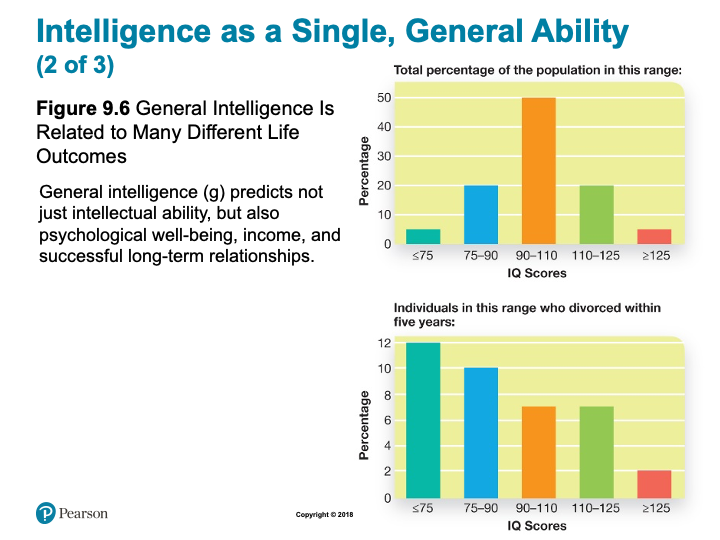
\includegraphics{assets/unit_2/slide_23.png}

\emph{Slide showing - General Intelligence Is Related to Many Different Life Outcomes}

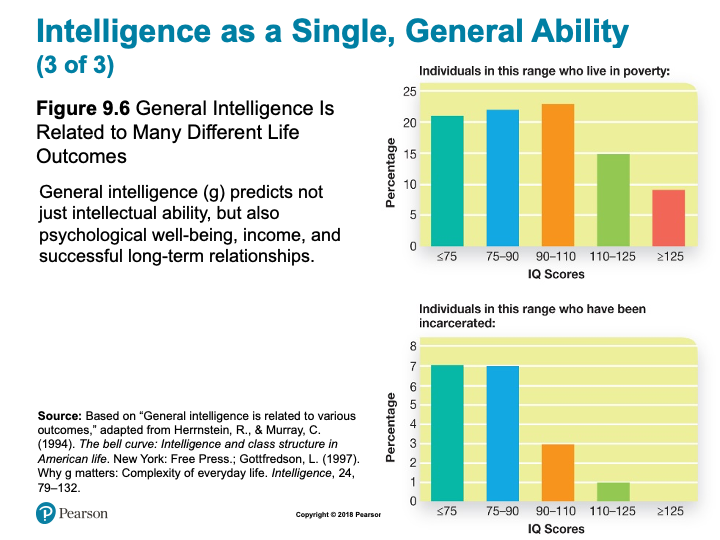
\includegraphics{assets/unit_2/slide_24.png}

\emph{Slide showing - General Intelligence Is Related to Many Different Life Outcomes}

Spearman's General Intelligence

\begin{itemize}
\tightlist
\item
  Does ``g'' tell us the whole story?
\end{itemize}

Intelligence as Multiple, Specific Abilities

\begin{itemize}
\tightlist
\item
  Spearman

  \begin{itemize}
  \tightlist
  \item
    Two factors: ``g'' and ``s''\\
  \end{itemize}
\item
  Thurstone

  \begin{itemize}
  \tightlist
  \item
    7 primary mental abilities\\
  \end{itemize}
\item
  Hierarchical model of intelligence

  \begin{itemize}
  \tightlist
  \item
    Nesting
  \end{itemize}
\end{itemize}

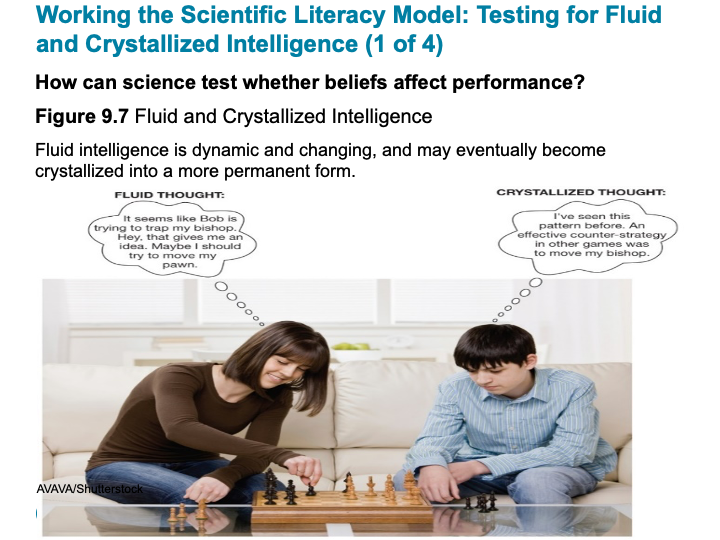
\includegraphics{assets/unit_2/slide_26.png}

\emph{Slide showing - Fluid and Crystallized Intelligence}

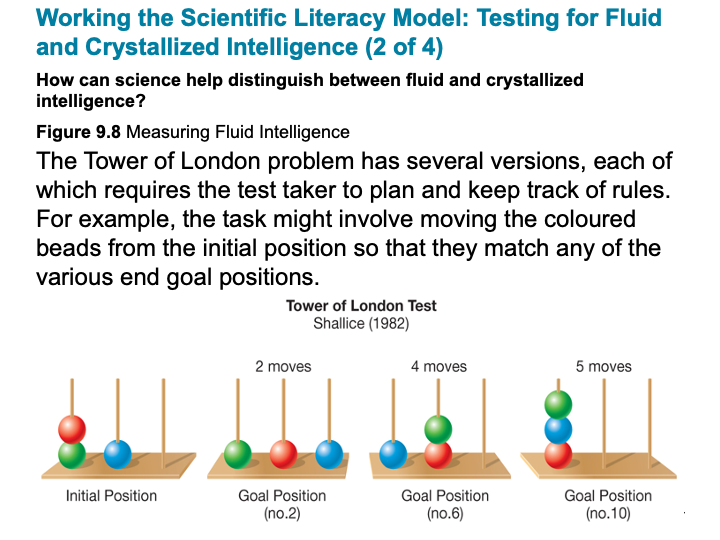
\includegraphics{assets/unit_2/slide_27.png}

\emph{Slide showing - Measuring Fluid Intelligence}

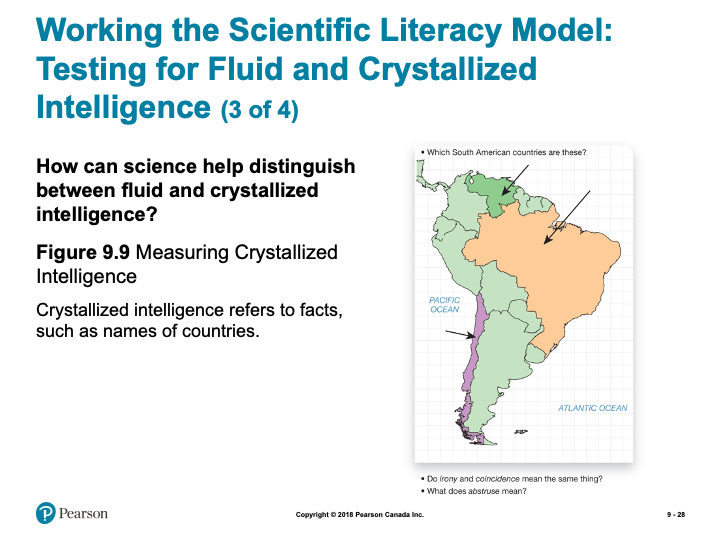
\includegraphics{assets/unit_2/slide_28.png}

\emph{Slide showing - Measuring Crystallized Intelligence}

\begin{itemize}
\tightlist
\item
  Can we critically evaluate crystalized and fluid intelligence?

  \begin{itemize}
  \tightlist
  \item
    Gf is a blend of several different cognitive abilities\\
  \item
    Gf and Gc are not entirely separable
  \end{itemize}
\end{itemize}

Why is this relevant?

\begin{itemize}
\tightlist
\item
  Stereotypes related to intelligence and age
\end{itemize}

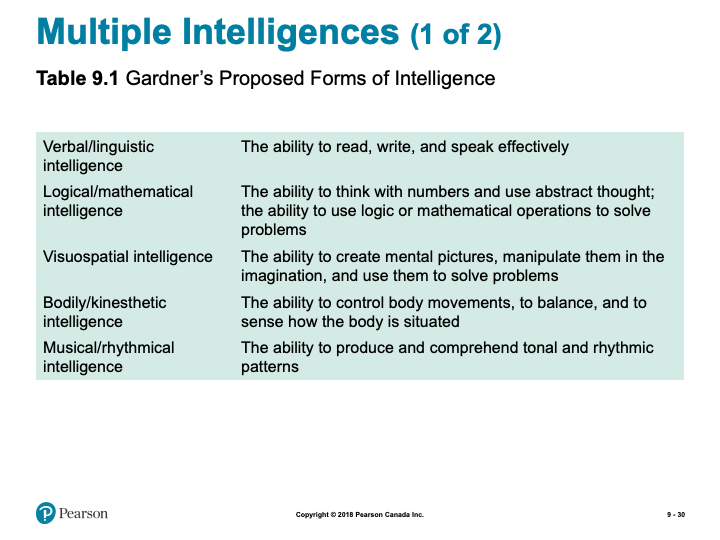
\includegraphics{assets/unit_2/slide_30.png}

\emph{Slide showing - Gardner's Proposed Forms of Intelligence}

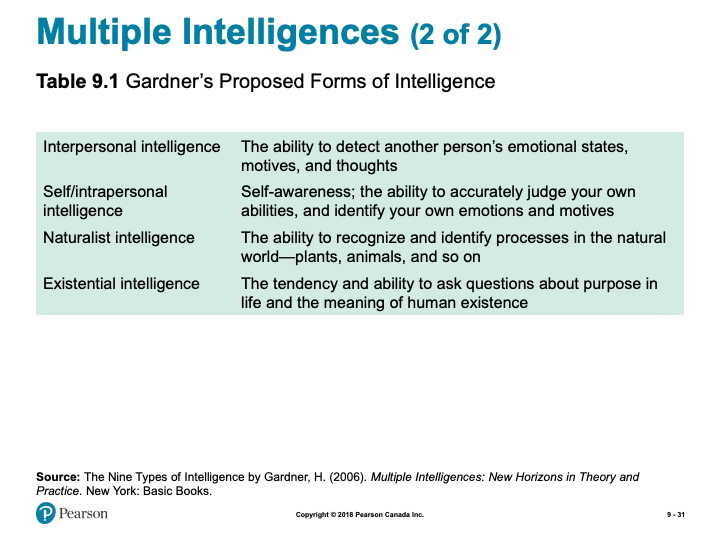
\includegraphics{assets/unit_2/slide_31.png}

\emph{Slide showing - Gardner's Proposed Forms of Intelligence}

Myths in Mind: Learning Styles

\begin{itemize}
\tightlist
\item
  Visual learners should learn more with visual materials?

  \begin{itemize}
  \tightlist
  \item
    Lack of supporting evidence\\
  \end{itemize}
\item
  Focus on learning the meaning
\end{itemize}

PSYCH @ The NHL

\begin{itemize}
\tightlist
\item
  Head injuries in the NHL\\
\item
  Chronic traumatic encephalopathy\\
\item
  ImPACT

  \begin{itemize}
  \tightlist
  \item
    Regular testing checks for declines on specific abilities
  \end{itemize}
\end{itemize}

The Battle of the Sexes?

\begin{itemize}
\tightlist
\item
  Differences in intelligence?

  \begin{itemize}
  \tightlist
  \item
    No sex differences found\\
  \item
    Male scores have greater variability
  \end{itemize}
\item
  Do males and females have unique cognitive abilities?

  \begin{itemize}
  \tightlist
  \item
    Females: verbal, memory, emotions\\
  \item
    Males: visuospatial\\
  \item
    Stereotype threat
  \end{itemize}
\end{itemize}

9.3 Learning Objectives

\begin{itemize}
\tightlist
\item
  Know the key terminology related to heredity, environment, and intelligence.\\
\item
  Understand different approaches to studying the genetic basis of intelligence.\\
\item
  Apply your knowledge of environmental and behavioural effects on intelligence to understand how to enhance your own cognitive abilities.\\
\item
  Analyze the belief that older children are more intelligent than their younger siblings.
\end{itemize}

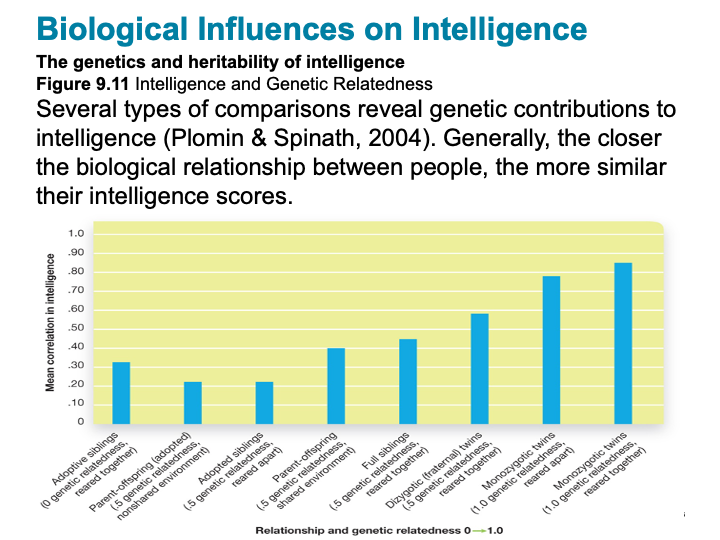
\includegraphics{assets/unit_2/slide_36.png}

\emph{Slide showing - Intelligence and Genetic Relatedness}

Working the Scientific Literacy Model: Brain Size and Intelligence

\begin{itemize}
\tightlist
\item
  What do we know about brain size and intelligence?

  \begin{itemize}
  \tightlist
  \item
    Once believed brain size was related to intelligence

    \begin{itemize}
    \tightlist
    \item
      Contributed to prejudice
    \end{itemize}
  \end{itemize}
\end{itemize}

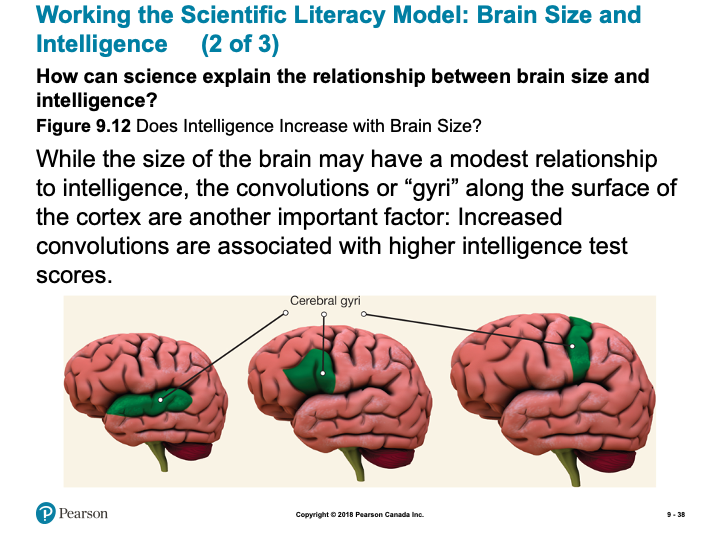
\includegraphics{assets/unit_2/slide_38.png}

\emph{Slide showing - Does Intelligence Increase with Brain Size?}

\begin{itemize}
\tightlist
\item
  Can we critically evaluate the issue?

  \begin{itemize}
  \tightlist
  \item
    Which abilities underlie the correlation?\\
  \item
    Third-variable problem
  \end{itemize}
\item
  Why is this relevant?

  \begin{itemize}
  \tightlist
  \item
    Brain size and IQ used to understand clinical conditions

    \begin{itemize}
    \tightlist
    \item
      Prolonged anorexia nervosa and alcohol abuse
    \end{itemize}
  \end{itemize}
\end{itemize}

Environmental Influences on Intelligence

\begin{itemize}
\tightlist
\item
  Nutrition\\
\item
  Socioeconomic Status (SES)\\
\item
  Stress\\
\item
  Birth Order\\
\item
  Education
\end{itemize}

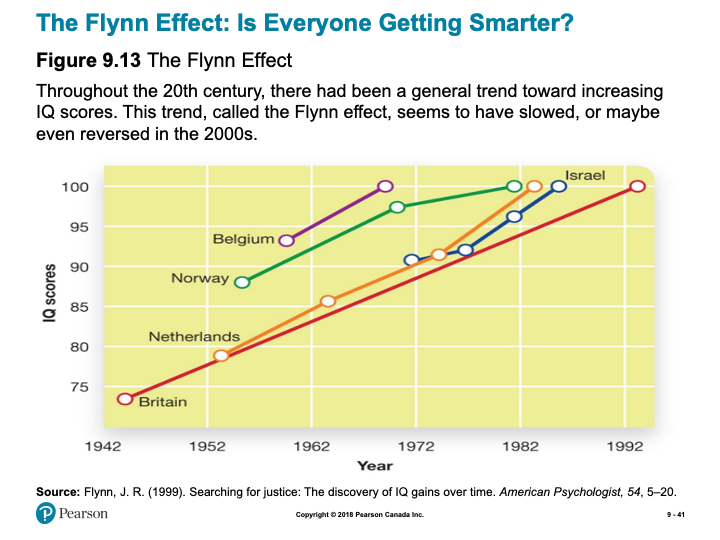
\includegraphics{assets/unit_2/slide_41.png}

\emph{Slide showing - The Flynn Effect}

Behavioural Influences on Intelligence

\begin{itemize}
\tightlist
\item
  Brain training programs\\
\item
  Nootropic drugs (p.~358)
\end{itemize}

\textbf{Note:} the slides are intended to supplement the information found in your textbook. If you are having trouble viewing them, they can also be downloaded by scrolling to the bottom of the screen and clicking on the ``Unit 2 - Slides'' link.*

{Intelligence Testing}

\begin{itemize}
\tightlist
\item
  Take some intelligence tests for yourself. As you complete them, consider how they might be considered beneficial, and controversial, as measures of intelligence.
\end{itemize}

{I.Q. Testing}

\begin{itemize}
\tightlist
\item
  Take some I.Q. Tests. Consider how valid and reliable these results are and think about how meaningful the results are.
\end{itemize}

{Ch. 9 Key Terms Quiz}

\begin{itemize}
\tightlist
\item
  Practice quiz to assess how well you know key terms from Chapter 9.\\
\item
  Not for formal evaluation.\\
\item
  Each topic will provide a question or scenario for you to consider prior to attending your Learning Lab. Be sure to carefully consider each prompt as you will be expected to contribute to the group discussion.
\end{itemize}
\end{reflect}

\hypertarget{resources-1}{%
\subsection*{Resources}\label{resources-1}}
\addcontentsline{toc}{subsection}{Resources}

Here are some additional resources that will help you complete this unit:

\begin{itemize}
\tightlist
\item
  Krause, M., Corts, D., Smith, S. C., \& Dolderman, D. (2018). \emph{Revel for An Introduction to Psychological Science, 2nd Canadian Edition.} Pearson Ed.\\
\item
  Other resources will be provided online.
\end{itemize}

\hypertarget{what-is-intelligence}{%
\section{What is Intelligence?}\label{what-is-intelligence}}

\hypertarget{intelligence}{%
\subsection*{Intelligence}\label{intelligence}}
\addcontentsline{toc}{subsection}{Intelligence}

As David Myers points out, intelligence is a slippery concept. We all have an idea of what it refers to, but we cannot agree on a single definition. Perhaps the most helpful advice is to remember, as Myers points out, that ``intelligence is a socially constructed concept. Cultures deem `intelligent' whatever attributes enable success in those cultures'' (2010). Historically, in North American culture, the idea of intelligence performance on an IQ test. The composition of these tests reflected North American culture's emphasis on particular mental abilities, specifically, those associated with success in an academic setting. More recently, we have come to realize that there are many kinds of intelligence. In this unit we will consider some varieties of intelligence, or multiple intelligences.

\hypertarget{types-of-intelligence}{%
\section*{Types of Intelligence}\label{types-of-intelligence}}
\addcontentsline{toc}{section}{Types of Intelligence}

\hypertarget{emotional-intelligence}{%
\subsection*{Emotional Intelligence}\label{emotional-intelligence}}
\addcontentsline{toc}{subsection}{Emotional Intelligence}

I have to admit that when I first heard of emotional intelligence (EI) I was skeptical. It sounded like popular psychology - someone trying to make a buck preying on our need for self-knowledge. However, upon further investigation I found that EI was linked to social intelligence (the ability to understand and relate to people), a concept developed by the pioneering psychologist E.L. Thorndike in 1920. And upon still further investigation, I found EI made a lot of sense.

\hypertarget{sternbergs-three-components-of-intelligence}{%
\subsection*{Sternberg's Three Components of Intelligence}\label{sternbergs-three-components-of-intelligence}}
\addcontentsline{toc}{subsection}{Sternberg's Three Components of Intelligence}

Robert Sternberg wanted to show that intelligence was more than just one general ability (known as \emph{g theory}). He believed our intelligence is best classified into three areas that predict real - world success: \textbf{\emph{analytical, creative, and practical.}} The following article does a great job explaining the Triarchic Theory of Intelligence and its three sub-theories. It also makes note of the criticisms that have been brought against this theory. \emph{To better understand Sternberg's Three Components of Intelligence follow the link below:}

\begin{itemize}
\tightlist
\item
  \href{https://www.thoughtco.com/triarchic-theory-of-intelligence-4172497}{\textbf{Three Components of Intelligence}}
\end{itemize}

\hypertarget{gardners-eight-types-of-intelligence}{%
\subsection*{Gardner's Eight Types of Intelligence}\label{gardners-eight-types-of-intelligence}}
\addcontentsline{toc}{subsection}{Gardner's Eight Types of Intelligence}

Howard Gardner put together a robust, research-based theory of Multiple Intelligences. He put forth an understanding of intelligence promoting our abilities are best classified into nine independent intelligences, which include a broad range of skills beyond traditional school smarts. This illuminating read that can help you understand what your primary intelligences are. Follow the link below:

\begin{itemize}
\tightlist
\item
  \href{https://www.institute4learning.com/resources/articles/multiple-intelligences/}{\textbf{Eight Types of Intelligence}}
\end{itemize}

\hypertarget{resources-online-articles-of-interest-2}{%
\subsection*{Resources: Online Articles of Interest}\label{resources-online-articles-of-interest-2}}
\addcontentsline{toc}{subsection}{Resources: Online Articles of Interest}

To add to your exploration of this topic, take a moment to read the following articles:

\begin{itemize}
\item
  \href{http://www.eiconsortium.org/}{\textbf{Emotional Intelligence Consortium Website}}
\item
  \href{http://eqi.org/}{\textbf{EQI Web Resource}}
\end{itemize}

\hypertarget{activity-intelligence-testing}{%
\subsection*{Activity: Intelligence Testing}\label{activity-intelligence-testing}}
\addcontentsline{toc}{subsection}{Activity: Intelligence Testing}

\begin{reflect}
In this unit we investigated Intelligence Testing. One of the important concepts we learned was that Intelligence Testing can be controversial due to its socially constructed nature.

Below is a link to a website that will allow you to take some Intelligence Tests for yourself. As you work through each test, and see the results, think about why we might consider these types of tests beneficial, and why they might be considered controversial.

\begin{itemize}
\tightlist
\item
  \href{https://www.queendom.com/tests/}{\textbf{Emotional Intelligence Test}}
\end{itemize}

{Learning Lab Preparation}

Our Learning Lab for this unit will focus on Intelligence Testing. As we have seen, Intelligence Testing is best implemented after careful consideration - this will be the focus of our discussion during this unit's Learning Lab. To help you prepare, consider the following questions:

\begin{itemize}
\tightlist
\item
  \textbf{\emph{How do you feel about the EMOTIONAL INTELLIGENCE TESTS? Did you learn anything? If so, what were the important areas that were illumined by the test?}}\\
\item
  \textbf{\emph{Is `emotional intelligence' a valid concept worth measuring?}}\\
\item
  \textbf{\emph{Do you believe E-IQ is more important than ``intelligence'' as measured by IQ scores for success and happiness in your life?''}}
\end{itemize}
\end{reflect}

\hypertarget{extremes-of-intelligence}{%
\section{Extremes of Intelligence}\label{extremes-of-intelligence}}

\hypertarget{iq-testing}{%
\subsection*{IQ Testing}\label{iq-testing}}
\addcontentsline{toc}{subsection}{IQ Testing}

In this section we continue to build upon our understanding of intelligence and testing to focus on Intelligence tests and those who score at the ``extremes.'' Intelligence tests are the most common tool used to measure intelligence. Intelligence test are one method of assessing an individual's mental aptitudes and comparing them with those of others using numerical scores. These scores are then plotted on a normal (bell) curve to estimate where a person's intelligence rates in relation to a standardized population. The extremes of intelligence is the understanding that on one end of the continuum are those with intellectual disabilities and on the other end are those who are geniuses.

\hypertarget{resources-2}{%
\subsection*{Resources}\label{resources-2}}
\addcontentsline{toc}{subsection}{Resources}

To supplement our understanding of this topic, take a moment to explore the following resources:

\begin{itemize}
\item
  \href{https://thearc.org/}{\textbf{The Arc}}
\item
  \href{https://www.mensa.org}{\textbf{MENSA International}}
\end{itemize}

\hypertarget{activity-iq-testing}{%
\subsection*{Activity: IQ Testing}\label{activity-iq-testing}}
\addcontentsline{toc}{subsection}{Activity: IQ Testing}

\begin{reflect}
After considering the above, and having read the textbook's discussion of intelligence testing, you might want to try some tests yourself. The value in doing this is not that you will get an accurate idea of your IQ score, but rather that you might get a better understanding for some of the problems in testing. As you try some of the tests at the following sites, remind yourself of the problems of test standardization, validity, and reliability. How well do you think these tests measure up?

\begin{itemize}
\tightlist
\item
  \href{https://www.queendom.com/tests/index.htm}{\textbf{Queendom IQ Test}}\\
\item
  \href{http://www.davideck.com/}{\textbf{davideck.com}}
\end{itemize}

{Learning Lab Preparation}

As we prepare for our Learning Lab this week, we consider intelligence from a Christian perspective. Read the following passage and carefully consider the questions below to help prepare for our discussion:

\emph{The Bible says, in James; Chapter 2:}

\emph{My brothers, as believers in our glorious Lord Jesus Christ, don't show favoritism. Suppose a man comes into your meeting wearing a gold ring and fine clothes, and a poor man in shabby clothes also comes in. If you show special attention to the man wearing fine clothes and say, ``Here's a good seat for you,'' but say to the poor man, ``You stand there'' or ``Sit on the floor by my feet,'' have you not discriminated among yourselves and become judges with evil thoughts?}

\begin{itemize}
\tightlist
\item
  \textbf{\emph{Could we be guilty of favoritism in esteeming more intelligent people above less intelligent people? In society? In Church?}}
\end{itemize}
\end{reflect}

\hypertarget{nature-nature-and-iq}{%
\section{Nature-Nature and IQ}\label{nature-nature-and-iq}}

While the debate rages over the relative contributions of nature and nurture to IQ, no one denies that heredity (nature) plays some role. The question arises then, ``So what?'' Are we going to try to control (and presumably increase) IQ through genetic engineering or some other method of eugenics (\emph{Eugenics is the search for hereditary factors that give people an evolutionary advantage; translated it can mean ``good genes'' or ``good origin''})? Are we going to control who should have children and how many, allowing the most intelligent parents to have more children and restricting the less intelligent? When the genetic basis for IQ (or some other component of intelligence) is identified, will parents select embryos with greater potential? For more on this topic see the following quote and the website from which it came.

``If we are concerned for the future of the (hopefully) millions of generations still to be born, we must realize that their fate lies to a considerable extent in the breeding practices of those who are currently alive.'' \emph{(Intelligence and Eugenics)}

\hypertarget{what-will-you-do}{%
\section{What Will You Do?}\label{what-will-you-do}}

If or when you have children, will you ban screens (TV, smart phone, tablet, laptop) as a ``brain rotter'' and read to them every day? Or will you just let nature take its course and allow both screens and reading?

\hypertarget{test-biases}{%
\section{Test Biases?}\label{test-biases}}

IQ tests are generally valid for their original purpose---as predictors of aca­demic performance. Controversy arises when IQ scores are taken to mean over­all intelligence and even overall worth. IQ scores consistently predict that some cultural and racial groups will do better at school than will other groups. These differ­ences are an indication of bias not in the IQ tests but in the back­grounds and academic settings that first create and then magnify differences.

\hypertarget{resources-3}{%
\subsection*{Resources}\label{resources-3}}
\addcontentsline{toc}{subsection}{Resources}

To supplement our understanding of this topic, take a moment to read through the following:

\begin{itemize}
\tightlist
\item
  \href{https://darkwing.uoregon.edu/~adoption/topics/naturenurturestudies.htm}{\textbf{The Adoption History Project}}\\
\item
  \href{http://unisci.com/stories/20012/0417014.htm}{\textbf{Nature-Nature and IQ}}
\end{itemize}

\hypertarget{activity-ch.-9-key-terms-quiz}{%
\subsection*{Activity: Ch. 9 Key Terms Quiz}\label{activity-ch.-9-key-terms-quiz}}
\addcontentsline{toc}{subsection}{Activity: Ch. 9 Key Terms Quiz}

\begin{reflect}
In order to review some of the major terms from Chapter 9 in your textbook, take the following unmarked quiz. Although you will not be evaluated on these terms, they will assist you in the assessments for this course:

{Learning Lab Preparation}

Consider the following scenario (and questions) as you continue to prepare for this unit's Learning Lab. You will be asked to share your thoughts so come prepared

*If you suggest that Asians have darker skin than Caucasians, you are not considered racist; this is an obvious fact with a genetic basis. However, if you suggest that Asians are more intelligent than Caucasians (as IQ tests show), or that African Americans are less intelligent, watch out

\begin{itemize}
\tightlist
\item
  \textbf{\emph{What is different about these two claims that makes us accept one and not the other? Is it the role of nature versus nurture? Or is it more closely tied to the high value our culture places on intelligence, and especially IQ scores?}}\\
\item
  \textbf{\emph{If IQ were unimportant would it matter if one racial or gender group tended to score higher than another group? Would you be considered racist or sexist for suggesting this?}}
\end{itemize}
\end{reflect}

\hypertarget{assessment-1}{%
\section*{Assessment}\label{assessment-1}}
\addcontentsline{toc}{section}{Assessment}

\begin{assessment}
While there is no ``formal'' assignment that you will be responsible for submitting for Unit 2, you will be expected to participate in discussion during your Learning Lab. Your facilitator will be providing a participation mark based on your contributions. Below is some information to consider prior to attending your Learning Lab:

\emph{Active participation in group exercises, reflection, and critical discourse is an essential component of this course. You are expected to show respect for all members of the course, both in your speech and actions. Contribute by actively observing and listening, raising thoughtful questions, examining relevant issues, building on others' ideas, analyzing and evaluating the group's thinking, synthesizing key points, and expanding the group's perspectives. Take care not to dominate a conversation, giving space for others to speak. When in small groups help maintain the focus, flow, and quality of conversations, and take the initiative to invite others (particularly those who are quiet) to speak.}

\textbf{Rubric for Participation in Learning Labs}

\begin{longtable}[]{@{}
  >{\raggedright\arraybackslash}p{(\columnwidth - 4\tabcolsep) * \real{0.3333}}
  >{\raggedright\arraybackslash}p{(\columnwidth - 4\tabcolsep) * \real{0.3333}}
  >{\raggedright\arraybackslash}p{(\columnwidth - 4\tabcolsep) * \real{0.3333}}@{}}
\toprule\noalign{}
\begin{minipage}[b]{\linewidth}\raggedright
Emerging (0-64\%)
\end{minipage} & \begin{minipage}[b]{\linewidth}\raggedright
Developing (65-89\%)
\end{minipage} & \begin{minipage}[b]{\linewidth}\raggedright
Mastering (90-100\%)
\end{minipage} \\
\midrule\noalign{}
\endhead
\bottomrule\noalign{}
\endlastfoot
Never to almost never: Demonstrates active listening (as indicated by disengaged body language and no to rare comments that build on others' remarks), Initiates any contributions in class or small groups, Makes insightful or constructive comments, Helps maintain a supportive space for others to speak. & Sometimes to fairly often: Demonstrates active listening (as indicated by somewhat to often engaged body language and comments that build on others' remarks), Initiates a contribution at least once in a class or small group discussion; Makes insightful or constructive comments, Helps maintain a supportive space for others to speak. & Very often to nearly always: Demonstrates active listening (as indicated by fully engaged body language and comments that build on others' remarks), Initiates more than one contribution in a class or small group discussion, Makes insightful or constructive comments, Creates a space for others to speak and takes initiative to include others. \\
\end{longtable}
\end{assessment}

\hypertarget{checking-your-learning-1}{%
\section*{Checking your Learning}\label{checking-your-learning-1}}
\addcontentsline{toc}{section}{Checking your Learning}

\begin{progress}
Before you move on to the next unit, check that you are able to:

\begin{itemize}
\tightlist
\item
  Define the key terminology associated with understanding intelligence, intelligence testing, and heredity, environment, and intelligence.\\
\item
  Understand the reasoning behind the eugenics movements and its use of intelligence tests, why intelligence is divided into fluid and crystallized types, and the genetic basis of intelligence.\\
\item
  Apply the concepts of entity theory and incremental theory to help kids succeed in school, to identify examples from the triarchic and multiple theories of intelligence, and to recognize environmental and behavioral effects on intelligence to understand how to enhance your own cognitive abilities.\\
\item
  Analyze why it is difficult to remove all cultural bias from intelligence testing and whether teachers should spend time tailoring lessons to each individual student's learning style.
\end{itemize}
\end{progress}

\hypertarget{the-developing-person---part-1}{%
\chapter{The Developing Person - Part 1}\label{the-developing-person---part-1}}

\hypertarget{overview-2}{%
\section*{Overview}\label{overview-2}}
\addcontentsline{toc}{section}{Overview}

Now that we have covered over some broad and influential topics in psychology, we begin our focus on human development. The focus of the content for this unit, will be on Chapter 10 in your textbook. As you turn ahead, you will notice that Chapter 10 contains a large amount of information - because of this, we will be covering it in this unit, and the next (Unit 4).

In this Unit (Part 1), you will learn about various strategies for researching human development, normal and abnormal prenatal development, and various cognitive, physical, and social developmental factors for infancy, childhood, and adolescence.

\hypertarget{topics-2}{%
\subsection*{Topics}\label{topics-2}}
\addcontentsline{toc}{subsection}{Topics}

This unit is divided into the following topics:

\begin{enumerate}
\def\labelenumi{\arabic{enumi}.}
\tightlist
\item
  Prenatal Development\\
\item
  Infancy and Childhood\\
\item
  Adolescence
\end{enumerate}

\hypertarget{learning-outcomes-2}{%
\subsection*{Learning Outcomes}\label{learning-outcomes-2}}
\addcontentsline{toc}{subsection}{Learning Outcomes}

By the end of this unit, student's will be able to:

\begin{itemize}
\tightlist
\item
  Define the key terminology related to prenatal and infant physical development, infancy and childhood, and adolescent development.\\
\item
  Understand advantages and disadvantages to different research designs in developmental psychology.\\
\item
  Understand the cognitive changes that occur during infancy and childhood, and the importance of attachment and the different styles of attachment.\\
\item
  Understand the process of identity formation, relationships, and moral emotions during adolescence.\\
\item
  Apply your understanding to identify the best ways expectant parents can ensure the health of their developing fetus, how to promote learning, and how to categorize moral reasoning.\\
\item
  Analyze the effects of preterm birth, how to effectively discipline children, and adolescent judgment and risk taking.
\end{itemize}

\hypertarget{activity-checklist-2}{%
\subsection*{Activity Checklist}\label{activity-checklist-2}}
\addcontentsline{toc}{subsection}{Activity Checklist}

Here is a checklist of learning activities you will benefit from in completing this unit. You may find it useful for planning your work:

\begin{reflect}
{Read and Reflect}

\begin{itemize}
\tightlist
\item
  Read \emph{Krause et al.~(2021). Revel for An Introduction to Psychological Science, 3rd Canadian Edition}\\
\item
  Continue our study of development - in particular, some of the major changes adolescents go through in their growth.\\
\item
  Review \emph{Unit 3 - Slides}
\end{itemize}

CLICK HERE

An Introduction to Psychological Science - Chapter 10:Lifespan Development

Learning Objectives

\textsuperscript{12} The righteous will flourish like a palm tree, they will grow like a cedar of Lebanon;\\
\textsuperscript{13} planted in the house of the Lord, they will flourish in the courts of our God.\\
\textsuperscript{14} They will still bear fruit in old age,they will stay fresh and green,\\
\textsuperscript{15} proclaiming, ``The Lord is upright; he is my Rock, and there is no wickedness in him.''\\
//todo \#11
- Video: \href{http://www.ted.com/talks/annie_murphy_paul_what_we_learn_before_we_re_born.html}{Annie Murphy Paul: What we learn before we're born}


\includegraphics{assets/unit_3/slide_3.png}

\emph{Slide showing - Introduction}

Modules

\begin{itemize}
\tightlist
\item
  Physical Development from Conception through Infancy\\
\item
  Infancy and Childhood: Cognitive and Emotional Development\\
\item
  Adolescence\\
\item
  Adulthood and Aging
\end{itemize}

Learning Objectivess

\begin{itemize}
\tightlist
\item
  Know the key terminology related to prenatal and infant physical development.\\
\item
  Understand pros and cons to different research designs in developmental psychology.\\
\item
  Apply your understanding to identify the best ways expectant parents can ensure the health of their developing fetus.\\
\item
  Analyze the effects of preterm birth.
\end{itemize}

Developmental Psychology

\begin{itemize}
\tightlist
\item
  Developmental psychology (p.~362)

  \begin{itemize}
  \tightlist
  \item
    Early development influences later behaviours
  \end{itemize}
\end{itemize}

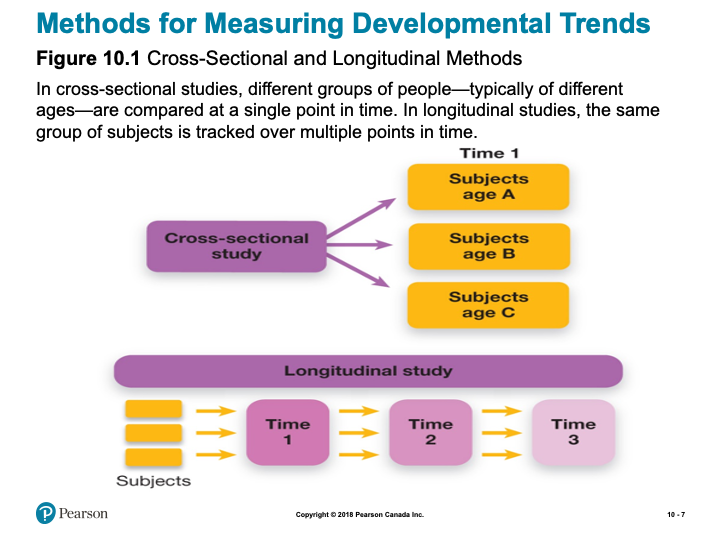
\includegraphics{assets/unit_3/slide_7.png}

\emph{Slide showing - Cross-Sectional and Longitudinal Methods}

Patterns of Development: Stages and Continuity

\begin{itemize}
\tightlist
\item
  Stages

  \begin{itemize}
  \tightlist
  \item
    Abrupt transitions\\
  \end{itemize}
\item
  Continuous

  \begin{itemize}
  \tightlist
  \item
    Slow changes
  \end{itemize}
\end{itemize}

\includegraphics{assets/unit_3/slide_9.png}

\emph{Slide showing - Phases of Prenatal Development}

\includegraphics{assets/unit_3/slide_10.png}

\emph{Slide showing - Fetal Brain Development}

Nutrition, Teratogens, and Fetal Development

\begin{itemize}
\tightlist
\item
  Teratogen (p.~366)

  \begin{itemize}
  \tightlist
  \item
    Alcohol\\
  \item
    Cigarettes\\
  \end{itemize}
\item
  Fetal Alcohol Syndrome (p.~366)

  \begin{itemize}
  \tightlist
  \item
    1.5 in 1000 worldwide

    \begin{itemize}
    \tightlist
    \item
      Likely higher\\
    \end{itemize}
  \end{itemize}
\item
  Stress
\end{itemize}

Working the Scientific Literacy Model: The Long-Term Effects of Premature Birth

\begin{itemize}
\tightlist
\item
  What do we know about premature birth?

  \begin{itemize}
  \tightlist
  \item
    Preterm infants (p.~368)\\
  \item
    25 weeks: 50\% survival\\
  \item
    30 weeks: 95\% survival\\
  \end{itemize}
\item
  How can science be used to help preterm infants?

  \begin{itemize}
  \tightlist
  \item
    NIDCAP\\
  \end{itemize}
\item
  Can we critically evaluate this research?

  \begin{itemize}
  \tightlist
  \item
    Small sample size\\
  \item
    Why does the program work?\\
  \end{itemize}
\item
  Why is this relevant?

  \begin{itemize}
  \tightlist
  \item
    9\% of infants are born preterm\\
  \item
    Simple interventions available:

    \begin{itemize}
    \tightlist
    \item
      Massage\\
    \item
      Kangaroo care
    \end{itemize}
  \end{itemize}
\end{itemize}

Myths in Mind: Vaccinations and Autism

\begin{itemize}
\tightlist
\item
  1990 claim that MMR vaccine linked to autism

  \begin{itemize}
  \tightlist
  \item
    One dose given at year 1\\
  \item
    Second does before starting school\\
  \item
    Many parents refused\\
  \end{itemize}
\item
  Lack of scientific support

  \begin{itemize}
  \tightlist
  \item
    Article retracted 2010
  \end{itemize}
\end{itemize}

Sensory Development in Infancy

\begin{itemize}
\tightlist
\item
  Sensory before birth

  \begin{itemize}
  \tightlist
  \item
    4 months gestation, brain receiving signals from eyes and ears\\
  \item
    7-8 months gestation, fetus actively listening\\
  \end{itemize}
\item
  Vision at birth

  \begin{itemize}
  \tightlist
  \item
    30 cm or less\\
  \item
    20/20 by 12 months\\
  \end{itemize}
\item
  Smell at birth

  \begin{itemize}
  \tightlist
  \item
    Cringe at foul odours\\
  \item
    Discriminate mother's breastmilk
  \end{itemize}
\end{itemize}

\includegraphics{assets/unit_3/slide_16.png}

\emph{Slide showing - Experimental Stimuli for Studying Visual Habituation in Infants}

\includegraphics{assets/unit_3/slide_17.png}

\emph{Slide showing - The Visual Cliff}

\includegraphics{assets/unit_3/slide_18.png}

\emph{Slide showing - A Few Key Infant Reflexes}

\includegraphics{assets/unit_3/slide_19.png}

\emph{Slide showing - Motor Skills Develop in Stages}

\includegraphics{assets/unit_3/slide_20.png}

\emph{Slide showing - The Processes of Synaptic Pruning}

Learning Objectives

\begin{itemize}
\tightlist
\item
  Know the key terminology associated with infancy and childhood.\\
\item
  Understand the cognitive changes that occur during infancy and childhood.\\
\item
  Understand the importance of attachment and the different styles of attachment.\\
\item
  Apply the concept of scaffolding and the zone of proximal development to understand how to best promote learning.\\
\item
  Analyze how to effectively discipline children in order to promote moral behaviour.
\end{itemize}

The Importance of Sensitive Periods

\begin{itemize}
\tightlist
\item
  Sensitive period (p.~375)

  \begin{itemize}
  \tightlist
  \item
    Language fluency\\
  \item
    Perception\\
  \item
    Balance\\
  \item
    Recognition of parents\\
  \item
    Identifying with a particular culture
  \end{itemize}
\end{itemize}

\includegraphics{assets/unit_3/slide_23.png}

\emph{Slide showing - Piaget's Stages of Cognitive Development}

The Sensorimotor Stage: Objects and the Physical World

\begin{itemize}
\tightlist
\item
  Sensorimotor stage (p.~375)

  \begin{itemize}
  \tightlist
  \item
    Birth to 2 years\\
  \item
    Object permanence (p.~376)

    \begin{itemize}
    \tightlist
    \item
      Hidden toy test
    \end{itemize}
  \end{itemize}
\end{itemize}

\includegraphics{assets/unit_3/slide_25.png}

\emph{Slide showing - Testing Conservation}

\includegraphics{assets/unit_3/slide_26.png}

\emph{Slide showing - Scale Errors and Testing for Scale Model Comprehension}

The Concrete Operational Stage: Using Logical Thought

\begin{itemize}
\tightlist
\item
  Concrete operational stage (p.~377)

  \begin{itemize}
  \tightlist
  \item
    7 to 11 years\\
  \item
    Transitivity
  \end{itemize}
\end{itemize}

The Formal Operational Stage: Abstract and Hypothetical Thought

\begin{itemize}
\tightlist
\item
  Formal operational stage (p.~378)

  \begin{itemize}
  \tightlist
  \item
    11 years to adulthood\\
  \item
    Scientific thinking
  \end{itemize}
\end{itemize}

Working the Scientific Literacy Model: Evaluating Piaget

\begin{itemize}
\tightlist
\item
  What do we know about cognitive abilities in infants?

  \begin{itemize}
  \tightlist
  \item
    Core knowledge hypothesis (p.~378)\\
  \item
    Habituation (p.~378)\\
  \item
    Dishabituation (p.~378)
  \end{itemize}
\end{itemize}

\includegraphics{assets/unit_3/slide_31.png}

\emph{Slide showing - Testing Infants' Understanding of Quantity}

Complementary Approaches to Piaget

\begin{itemize}
\tightlist
\item
  Vygotsky

  \begin{itemize}
  \tightlist
  \item
    Zone of proximal development (p.~380)

    \begin{itemize}
    \tightlist
    \item
      Scaffolding (p.~380)

      \begin{itemize}
      \tightlist
      \item
        Cultural differences
      \end{itemize}
    \end{itemize}
  \end{itemize}
\end{itemize}

Social Development and Attachment

\begin{itemize}
\tightlist
\item
  Attachment (p.~381)\\
\item
  Harry Harlow's monkey experiments\\
\item
  Strange situation test (p.382)
\end{itemize}

\includegraphics{assets/unit_3/slide_34.png}

\emph{Slide showing - The Strange Situation}

Social Development and Attachment

\begin{itemize}
\tightlist
\item
  Types of Attachment

  \begin{itemize}
  \tightlist
  \item
    Secure attachment

    \begin{itemize}
    \tightlist
    \item
      Insecure attachment\\
    \item
      Disorganized\\
    \item
      Anxious/Ambivalent\\
    \item
      Avoidant\\
    \end{itemize}
  \end{itemize}
\item
  Parenting and Attachment\\
\item
  Attachment behavioural system (p.~383)\\
\item
  Caregiving behavioural system (p.~383)\\
\item
  Conditional approaches\\
\item
  Introjection (p.~383)\\
\item
  Inductive discipline (p.~383)
\end{itemize}

Self-Awareness

\begin{itemize}
\tightlist
\item
  Self-awareness (p.~384)

  \begin{itemize}
  \tightlist
  \item
    Reflection in mirror\\
  \end{itemize}
\item
  Egocentric (p.~384)
\end{itemize}

\includegraphics{assets/unit_3/slide_38.png}

\emph{Slide showing - Piaget's Test for Egocentric Perspective in Children}

\begin{itemize}
\tightlist
\item
  Theory of mind (p.~384)\\
\item
  False-belief task
\end{itemize}

Psychosocial Development Across the Lifespan

\begin{itemize}
\tightlist
\item
  Infancy

  \begin{itemize}
  \tightlist
  \item
    Sense of security\\
  \end{itemize}
\item
  Toddlerhood

  \begin{itemize}
  \tightlist
  \item
    Exploring autonomy\\
  \end{itemize}
\item
  Early Childhood

  \begin{itemize}
  \tightlist
  \item
    Pushing boundaries and experimenting\\
  \end{itemize}
\item
  Childhood

  \begin{itemize}
  \tightlist
  \item
    Active engagement
  \end{itemize}
\end{itemize}

Learning Objectives

\begin{itemize}
\tightlist
\item
  Know the key terminology concerning adolescent development.\\
\item
  Understand the process of identity formation during adolescence.\\
\item
  Understand the importance of relationships in adolescence.\\
\item
  Understand the functions of moral emotions.\\
\item
  Apply your understanding of the categories of moral reasoning.\\
\item
  Analyze the relationship between brain development and adolescent judgment and risk taking.
\end{itemize}

\includegraphics{assets/unit_3/slide_42.png}

\emph{Slide showing - Physical Changes That Accompany Puberty in Male and Female Adolescents}

Emotional Challenges in Adolescence

\begin{itemize}
\tightlist
\item
  Intense and volatile emotions\\
\item
  Cognitive reframing\\
\item
  Ability to delay gratification (p.~392)
\end{itemize}

Working the Scientific Literacy Model: Adolescent Risk and Decision Making

\begin{itemize}
\tightlist
\item
  What do we know about adolescence and decision making?

  \begin{itemize}
  \tightlist
  \item
    Ongoing changes in prefrontal cortex

    \begin{itemize}
    \tightlist
    \item
      Region involved in impulse control, mood, planning, organizing, and reasoning
    \end{itemize}
  \end{itemize}
\end{itemize}

\includegraphics{assets/unit_3/slide_45.png}

\emph{Slide showing - Extended Brain Development}

\begin{itemize}
\tightlist
\item
  Can we critically evaluate this explanation for risky decision making?

  \begin{itemize}
  \tightlist
  \item
    Still capable of making good decisions\\
  \item
    Temperament and personality\\
  \item
    Situational factors\\
  \end{itemize}
\item
  Why is this relevant?

  \begin{itemize}
  \tightlist
  \item
    Major public health problem
  \end{itemize}
\end{itemize}

\includegraphics{assets/unit_3/slide_47.png}

\emph{Slide showing - What Drives Teenagers to Take Risks?}

Cognitive Development: Moral Reasoning vs.~Emotions

\begin{itemize}
\tightlist
\item
  Formal operational stage

  \begin{itemize}
  \tightlist
  \item
    Abstract thinking\\
  \item
    Scientific thinking\\
  \item
    Perspective taking
  \end{itemize}
\end{itemize}

Kohlberg's Moral Development: Learning Right from Wrong

\begin{itemize}
\tightlist
\item
  A trolley is hurtling down the tracks toward a group of five unsuspecting people. You are standing next to a lever that, if pulled, would direct the trolley onto another track, thereby saving the five individuals. However, on the second track stands a single, unsuspecting person, who would be struck by the diverted trolley.
\end{itemize}

\includegraphics{assets/unit_3/slide_50.png}

\emph{Slide showing - Kohlberg's Stages of Moral Reasoning}

Moral Development

\begin{itemize}
\tightlist
\item
  Social intuitionist model

  \begin{itemize}
  \tightlist
  \item
    Julie and Steven are brother and sister. They are travelling together in France on summer vacation from college. One night they are staying alone in a cabin near the beach. They decide that it would be interesting and fun if they shared a romantic kiss. At the very least it would be a new experience for each of them. They both enjoy the experience, but they decide not to do it again. They keep that night as a special secret, which makes them feel even closer to each other.
  \end{itemize}
\end{itemize}

Social Development: Identity and Relationships

\begin{itemize}
\tightlist
\item
  Identity (p.~395)

  \begin{itemize}
  \tightlist
  \item
    Personal qualities\\
  \item
    Social qualities\\
  \item
    Future goals\\
  \end{itemize}
\item
  Adolescence identity crisis

  \begin{itemize}
  \tightlist
  \item
    Curiosity, questioning, and exploration\\
  \end{itemize}
\item
  Peer groups\\
\item
  Romantic relationships
\end{itemize}

Learning Objectives

\begin{itemize}
\tightlist
\item
  Know the key terminology concerning adulthood and aging.\\
\item
  Know the key areas of growth experiences by emerging adults.\\
\item
  Understand age-related disorders such as Alzheimer's disease.\\
\item
  Understand how cognitive abilities change with age.\\
\item
  Apply your attitudes about marriage.\\
\item
  Analyze the stereotype that old age is a time of unhappiness.
\end{itemize}

Physical Changes in Adulthood

\begin{itemize}
\tightlist
\item
  Age brackets:

  \begin{itemize}
  \tightlist
  \item
    Young adulthood: 18-40 years\\
  \item
    Middle adulthood: 40-65 years\\
  \item
    Older adulthood: 65 years and onward\\
  \end{itemize}
\item
  Menopause (p.~399)
\end{itemize}

Psychosocial Development Across the Lifespan

\begin{itemize}
\tightlist
\item
  Ages 25 to 40

  \begin{itemize}
  \tightlist
  \item
    Separate from parents
  \item
    Work on intimate relationships
  \item
    Failure can result in isolation
  \end{itemize}
\item
  Ages 45 to 65
\item
  Producing something of value
\item
  Work and/or family
\item
  Ages 65+
\item
  Reflect on life of fulfillment (or not)
\end{itemize}

Love and Marriage

\begin{itemize}
\tightlist
\item
  Most adults pursue some kind of long-term relationship
\item
  Marriage associated with longer life, happiness
\item
  Gottman

  \begin{itemize}
  \tightlist
  \item
    Conflict and communication
  \item
    ``Four horsemen of the Apocalypse''
  \end{itemize}
\end{itemize}

Parenting

\begin{itemize}
\tightlist
\item
  Shift in identity, lifestyle
\item
  Children affect marriage
\item
  Empty nest myth
\end{itemize}

\includegraphics{assets/unit_3/slide_58.png}

\emph{Slide showing - Emotion, Memory, and Aging}

PSYCH @ The Driver's Seat

\begin{itemize}
\tightlist
\item
  Driving skills and age
\item
  UFOV Speed of Processing training

  \begin{itemize}
  \tightlist
  \item
    Computer-based
  \item
    Decreases accident risk
  \end{itemize}
\end{itemize}

\includegraphics{assets/unit_3/slide_60.png}

\emph{Slide showing - How Alzheimer's Disease Affects the Brain}

Working the Scientific Literacy Model: Aging and Cognitive Change

\begin{itemize}
\tightlist
\item
  What do we know about cognitive abilities?

  \begin{itemize}
  \tightlist
  \item
    Fluid intelligence declines
  \item
    Crystalized intelligence remains largely intact
  \end{itemize}
\item
  How can science explain age-related differences in cognitive abilities?

  \begin{itemize}
  \tightlist
  \item
    Activation of brain areas
  \end{itemize}
\end{itemize}

Working the Scientific Literacy Model: Aging and Cognitive Change

\begin{itemize}
\tightlist
\item
  Can we critically evaluate our assumptions about age-related cognitive changes?

  \begin{itemize}
  \tightlist
  \item
    Too simplistic to say memory declines

    \begin{itemize}
    \tightlist
    \item
      Many different types of memory
    \end{itemize}
  \item
    Compensation
  \end{itemize}
\item
  Why is this relevant?

  \begin{itemize}
  \tightlist
  \item
    Control over how one ages
  \end{itemize}
\end{itemize}

\includegraphics{assets/unit_3/slide_63.png}

\emph{Slide showing - Memory and Aging}

\textbf{Note:} The slides are intended to supplement the information found in your textbook. If you are having trouble viewing them, they can also be downloaded by scrolling to the bottom of the screen and clicking on the ``Unit 3 - Slides'' link.

{Designer Babies}

\begin{itemize}
\tightlist
\item
  Explore and reflect upon this contemporary and controversial issue. Designer babies pose many ethical issues and requires careful consideration.
\end{itemize}

{Cognitive Change}

\begin{itemize}
\tightlist
\item
  Reflect on your own development before taking a ``test'' to develop additional insights into your own developmental trajectory.
\end{itemize}

{Terminology Practice}

\begin{itemize}
\tightlist
\item
  Take this flip-card activity to self-evaluate how well you know some of the important terms from Chapter 10.
\end{itemize}

{Learning Lab Preparation}

\begin{itemize}
\tightlist
\item
  Each topic will provide a question or scenario for you to consider prior to attending your Learning Lab. Be sure to carefully consider each prompt as you will be expected to contribute to the group discussion.
\end{itemize}
\end{reflect}

\hypertarget{resources-4}{%
\subsection*{Resources}\label{resources-4}}
\addcontentsline{toc}{subsection}{Resources}

Here are some additional resources that will help you complete this unit:

\begin{itemize}
\tightlist
\item
  Krause, M., Corts, D., Smith, S. C., \& Dolderman, D. (2018). \emph{Revel for An Introduction to Psychological Science, 2nd Canadian Edition.} Pearson Ed.\\
\item
  Other resources will be provided online.
\end{itemize}

\hypertarget{prenatal-development}{%
\section{Prenatal Development}\label{prenatal-development}}

\hypertarget{physical-development}{%
\subsection*{Physical Development}\label{physical-development}}
\addcontentsline{toc}{subsection}{Physical Development}

Prenatal development is a time of rapid growth and change. This rapid change continues throughout the first few years of life. Development during early life is clearly a function both of nature and of the environment.

\hypertarget{questions-to-consider}{%
\subsection*{Questions to Consider}\label{questions-to-consider}}
\addcontentsline{toc}{subsection}{Questions to Consider}

After you have read the first few pages of this chapter you should be able to answer the following questions:

\begin{itemize}
\tightlist
\item
  \textbf{\emph{How is the gender of an offspring determined?}}\\
\item
  \textbf{\emph{What differentiates zygotes from embryos and embryos from fetuses?}}
\end{itemize}

\emph{(These questions are intended for personal reflection - you are not intended to submit anything for assessment)}

\hypertarget{designer-babies}{%
\subsection*{Designer Babies}\label{designer-babies}}
\addcontentsline{toc}{subsection}{Designer Babies}

It is beginning to look inevitable that, however fierce the debate, the technology to make designer babies will happen - maybe just 20 years from now. Geneticists claim to have found the gene for good-parenting, genes for obesity, Alzheimer's, red hair, and even happiness. Incredibly, scientists have even constructed an artificial human chromosome, which could carry any genes a geneticist - or prospective parents - desired.

Embryo A technique called Pre-implantation Genetic Diagnosis (PGD) is already being used to screen embryos for genetic diseases. Embryos created outside the body using in vitro fertilization are tested to see whether they carry a genetic disorder before being transferred to the uterus. It's deeply controversial whether parents should ever be allowed to select embryos just because they're genetically different.

At the moment the technique is used for therapeutic purposes only, to screen for children who may have a deadly genetic disease. Even if some parents and their doctors were willing to use PGD for cosmetic or enhancement purposes, which remains absolutely taboo, the technique is limited in a crucial way - PGD can only select an embryo with genes inherited from the parents.

\textbf{\emph{Bottled Genes?}} \emph{One day parents may be able to pick any gene they desire from a range of bottled genes and have it put into their embryos. (quoted from ``Designer Babies'' website)}

\hypertarget{activity-designer-babies}{%
\subsection*{Activity: Designer Babies}\label{activity-designer-babies}}
\addcontentsline{toc}{subsection}{Activity: Designer Babies}

\begin{reflect}
This activity involves some reading and reflection around the topic of genetic engineering. As this is a contemporary issue, it will be valuable to familiarize yourself with some of the complexities of this technology and think critically about some of the ethical challenges. Your task is to read the following resources and carefully consider the implications of this technology:

\begin{itemize}
\tightlist
\item
  \href{https://www.statnews.com/2019/09/16/could-editing-the-dna-of-embryos-with-crispr-help-save-people-who-are-already-alive/}{\textbf{Editing the DNA of Embryos with CRISPR}}\\
\item
  \href{https://www.geneticsandsociety.org/internal-content/designer-babies-crispr-genetic-engineering}{\textbf{Designer Babies, CRISPR, \& Genetic Engineering}}
\end{itemize}

{Learning Lab Preparation}

Prior to your Learning Lab, take some time to think about the following scenario and questions. You will be asked to share your thoughts in this week's Learning Lab:

\emph{Modern techniques of conception and human genetic engineer­ing raise important new issues for human development. A pam­phlet containing the following message was left at doorsteps in TWU professor Philipchalk's neighborhood:}

\includegraphics{assets/unit_3/U3_T1_LearningACtivitity.JPG}

\emph{Image showing an example of surrogacy message }

(\emph{You may also wish to comment on the ``Designer Babies'' topic above.})

\begin{enumerate}
\def\labelenumi{\arabic{enumi}.}
\tightlist
\item
  \textbf{\emph{How do you feel about this request?}}
\item
  \textbf{\emph{What problems might you anticipate?}}
\end{enumerate}
\end{reflect}

\hypertarget{infancy-and-childhood}{%
\section{Infancy and Childhood}\label{infancy-and-childhood}}

\hypertarget{a-childs-view-of-god}{%
\subsection*{A Child's View of God}\label{a-childs-view-of-god}}
\addcontentsline{toc}{subsection}{A Child's View of God}

One evening on a camping trip several years ago, my wife and I listened outside the tent as our five-year-old Joelle and three-year-old Matthew tried to get to sleep. Always the ``mother,'' Joelle attempted to dispel her little brother's fear of bears and other wild creatures by reminding him that Jesus was watching over them. Not content with generalities, Matt responded, ``Does Jesus got a gun?'' \emph{(Psychology and Christianity by Ronald Philipchalk, p.~141)}

As any Sunday School teacher knows, children see God differently from adults---often in very concrete terms (protection requires a gun!). Studying cognitive development can help us to understand as well as teach children at their own level.

\hypertarget{the-process-of-cognitive-change}{%
\subsection*{The Process of Cognitive Change}\label{the-process-of-cognitive-change}}
\addcontentsline{toc}{subsection}{The Process of Cognitive Change}

Our textbook provides a good summary of the structure (stages) of cognitive development. The section, however, does not address the process by which a person moves from one stage to the next. Piaget believed that the key to cognitive development is something called cognitive conflict or cognitive disequilibrium. For cognitive development to proceed, the individual must constantly re-evaluate his or her schemas. According to Piaget, we develop schemas from an early age of life. Schemas are our cognitive representations of the world. Schemas help us to organize our experiences. They also allow us to make predictions about what outcomes might result from particular behaviours. Schemas are very important in helping us to understand and to adapt to the world.

Although schemas are important in helping us to understand the world, they are not always accurate. People at all ages can have mental representations of the world that are not correct.

\textbf{\emph{Can you think of any examples of inaccurate schemas?}}

Although people at all ages can have inaccurate mental representations of the world, children are especially prone to view the world in an incorrect way. The reason children may view the world in an incorrect way is because the structure of their cognitive processing is developing. Piaget believed that inaccurate schemas are changed only when they are challenged in the cognitive structure of the child. This challenge has been termed cognitive conflict.

Basically, the process of cognitive change works as follows:

\begin{itemize}
\tightlist
\item
  People are motivated to maintain a state of cognitive equilibrium.\\
\item
  When a child encounters information from the world and the information is inconsistent with his or her schema, the new piece of information creates a state of disequilibrium or cognitive conflict.\\
\item
  \textbf{\emph{Equilibrium}} may be restored through one of the two processes of adapation called assimilation and accommodation.\\
\item
  \textbf{\emph{Assimilation}} occurs when a child re-organizes the new information in such a way as to make the new piece of information consistent with his or her preexisting schema of the world.\\
\item
  \textbf{\emph{Accommodation}} occurs when a child alters his or her schema such that the new piece of information can now be incorporated into the new schema.
\end{itemize}

Thus the process of accommodation produces the greatest cognitive change. Can you think of examples of both assimilation and accommodation? Here is an example:

\textbf{Equilibrium-Preexisting Schema:} Child has grown up in an environment where all people he interacted with were of the same race (mom, dad, siblings, grandma, grandpa, etc.) Child has seen people of other racial groups, but has never interacted with them. Child develops the schema that people tend to like others who are of the same race as him or her.

\textbf{Cognitive Conflict Produced:} At four years of age the child begins to attend preschool. At this time he starts to interact with children of various races. The child begins to develop a friendship with a child of a different race. This friendship creates cognitive conflict for the child: ``How can I like someone who is a different color?'' To resolve this cognitive conflict, the child has two options:

\textbf{\emph{Option A}}- \textbf{Assimilation:} In order to maintain his or her preexisting schema, the child re-organizes the information such that the other child is not perceived to be so dissimilar after all: ``Maybe he is a different color from me, but we both speak English. We must not be so dissimilar after all.''

\textbf{\emph{Option B}}- \textbf{Accommodation:} The child's preexisting schema is altered such that the new information can be incorporated into a new way of perceiving the world, ``Maybe I can be friends with someone who is different from me.''

\hypertarget{cognitive-equilibrium-is-restored}{%
\subsection*{Cognitive Equilibrium is Restored}\label{cognitive-equilibrium-is-restored}}
\addcontentsline{toc}{subsection}{Cognitive Equilibrium is Restored}

Although cognitive equilibrium is restored via either assimilation or accommodation, assimilation serves to maintain an inaccurate schema (that differences inhibit the development of friendships) whereas accommodation serves to produce cognitive change and hence produces a more accurate representation of the world (that differences do not inhibit the development of friendships).

\hypertarget{activitycognitive-change}{%
\subsection*{Activity:Cognitive Change}\label{activitycognitive-change}}
\addcontentsline{toc}{subsection}{Activity:Cognitive Change}

\begin{reflect}
The first three links below are articles that are intended to give you an opportunity to reflect upon your own considerations around development. The last link is a test - along with the first three links, it is intended to provide some insights about your developmental trajectory in light of your crisis resolution, attachment style, and parenting styles:

\begin{itemize}
\tightlist
\item
  \href{http://www.childdevelopmentinfo.com/development/erickson.shtml}{\textbf{Erik Erikson's Stages of Social-Emotional Development}}\\
\item
  \href{http://www.attachmentdisorder.net/}{\textbf{The Link Between Substance Abuse and Attachment Disorder}}\\
\item
  \href{https://www.mayoclinic.org/healthy-lifestyle/childrens-health/in-depth/stepfamilies/art-20047046}{\textbf{Stepfamilies: How to Help Your Child Adjust}}\\
\item
  \href{https://www.3smartcubes.com/pages/tests/parentingstyle/parentingstyle_instructions/}{\textbf{What is Your Parenting Style}}
\end{itemize}

{Learning Lab Preparation}

Prior to your Learning Lab, take some time to think about the following questions. You will be asked to share your thoughts in this week's Learning Lab:

\begin{itemize}
\tightlist
\item
  \textbf{\emph{What is God like for children of different levels of cognitive development? If you can, give some examples from children you know\ldots.}}\\
\item
  \textbf{\emph{Would children even have an idea of God if they were not taught it?}}
\end{itemize}
\end{reflect}

\hypertarget{adolescence}{%
\section{Adolescence}\label{adolescence}}

John has just turned 13. Over the past year he has experienced may changes. He has grown over six inches and he has developed acne over his face and back. Not only is he changing physically, he is also experiencing a wave of emotional, spiritual, cognitive, and sexual changes. John has become self-focused and very self-critical. In addition, he is beginning to think abstractly and to challenge adults' ``dominion'' on knowledge. John is also on a quest to understand ``who he is'' and ``what his place is in the world''. John's quest for an identity makes him more vulnerable to peer pressure and to the influence of radical groups and cults. During this time that we call adolescence, John will make many decisions that will have a profound effect on the direction his life will take.

\emph{Does any of the above sound familiar?}

Before you begin reading the textbook section on adolescence, think back to your own adolescence. As you think about your experience of adolescence, use the following questions to guide your reflection:

\begin{itemize}
\tightlist
\item
  What physical changes did you experience in adolescence?\\
\item
  How did these physical changes make you feel?\\
\item
  In what ways did your view of the world change during adolescence?\\
\item
  How did your way of treating other people change during adolescence?\\
\item
  What was most important to you during adolescence?\\
\item
  To what extent is ``who you are today'' a function of ``who you became during adolescence''?
\end{itemize}

\hypertarget{no-adolescence}{%
\subsection*{No Adolescence?}\label{no-adolescence}}
\addcontentsline{toc}{subsection}{No Adolescence?}

In other times and in other cultures to­day, adolescence does not exist as a significant and distinct period of develop­ment. This might seem surprising and difficult to imagine. Think of how modern society would be different, or if it could even exist, without a period of adolescence. What are the advantages and disadvantages of having an adolescent period?

\hypertarget{identity}{%
\subsection*{Identity}\label{identity}}
\addcontentsline{toc}{subsection}{Identity}

The concept of identity is a rich topic for consideration. The most familiar aspect of identity is occupational identity, since much of ``who we are'' in our society rests on the kind of work we do. Perhaps you can readily relate to this in your choice of major. Less familiar, but equally important, is ideological identity. Ideologi­cal identity, including both religious and political orientations, may un­dergo a tremen­dous upheaval during your student years. Do you have the same political beliefs as your parents? What about religious beliefs? Conflict and questioning of parental beliefs and values may be a necessary part of establishing your personal iden­tity---even if the beliefs and values you ultimately adopt are the same as those of your parents.

\hypertarget{learning-activities-1}{%
\subsection*{Learning Activities}\label{learning-activities-1}}
\addcontentsline{toc}{subsection}{Learning Activities}

\begin{reflect}
{Read and Reflect}

In this section we explore adolescence and the changes in development we go through. Below are some resources that help to help support your understanding:

\begin{itemize}
\tightlist
\item
  \href{https://www.sciencedirect.com/journal/journal-of-adolescence}{\textbf{Journal of Adolescence}}\\
\item
  \href{https://childdevelopmentinfo.com/child-development/erickson/\#gs.d8mpcv}{\textbf{Erik Erikson's Stages of Social-Emotional Development}}\\
\item
  \href{http://drjamesdobson.org/quiz/parenting-quiz/4-tips-for-parenting-teenagers}{\textbf{4 Tips for Parenting Teenagers}}
\end{itemize}

{Terminology Practice}

In order to review some of the major terms from Chapter 10 in your textbook, practice using the activity below. Although you will not be evaluated on these terms, they will assist you in the assessments for this course:

{Learning Lab Preparation}

Prior to your Learning Lab, take some time to think about the following questions. You will be asked to share your thoughts in this week's Learning Lab:

\begin{itemize}
\tightlist
\item
  \textbf{\emph{Would you want to live your adolescence over again if you could? Why or why not?}}
\end{itemize}
\end{reflect}

\hypertarget{assessment-2}{%
\section*{Assessment}\label{assessment-2}}
\addcontentsline{toc}{section}{Assessment}

\begin{assessment}
While there is no ``formal'' assignment that you will be responsible for submitting for Unit 3, you will be expected to participate in discussion during your Learning Lab. Your facilitator will be providing a participation mark based on your contributions. Below is some information to consider prior to attending your Learning Lab:

\emph{Active participation in group exercises, reflection, and critical discourse is an essential component of this course. You are expected to show respect for all members of the course, both in your speech and actions. Contribute by actively observing and listening, raising thoughtful questions, examining relevant issues, building on others' ideas, analyzing and evaluating the group's thinking, synthesizing key points, and expanding the group's perspectives. Take care not to dominate a conversation, giving space for others to speak. When in small groups help maintain the focus, flow, and quality of conversations, and take the initiative to invite others (particularly those who are quiet) to speak.}

\textbf{Rubric for Participation in Learning Labs}

\begin{longtable}[]{@{}
  >{\raggedright\arraybackslash}p{(\columnwidth - 4\tabcolsep) * \real{0.3333}}
  >{\raggedright\arraybackslash}p{(\columnwidth - 4\tabcolsep) * \real{0.3333}}
  >{\raggedright\arraybackslash}p{(\columnwidth - 4\tabcolsep) * \real{0.3333}}@{}}
\toprule\noalign{}
\begin{minipage}[b]{\linewidth}\raggedright
Emerging (0-64\%)
\end{minipage} & \begin{minipage}[b]{\linewidth}\raggedright
Developing (65-89\%)
\end{minipage} & \begin{minipage}[b]{\linewidth}\raggedright
Mastering (90-100\%)
\end{minipage} \\
\midrule\noalign{}
\endhead
\bottomrule\noalign{}
\endlastfoot
Never to almost never: Demonstrates active listening (as indicated by disengaged body language and no to rare comments that build on others' remarks),Initiates any contributions in class or small groups, Makes insightful or constructive comments, Helps maintain a supportive space for others to speak. & Sometimes to fairly often: Demonstrates active listening (as indicated by somewhat to often engaged body language and comments that build on others' remarks), Initiates a contribution at least once in a class or small group discussion; Makes insightful or constructive comments, Helps maintain a supportive space for others to speak. & Very often to nearly always: Demonstrates active listening (as indicated by fully engaged body language and comments that build on others' remarks), Initiates more than one contribution in a class or small group discussion, Makes insightful or constructive comments, Creates a space for others to speak and takes initiative to include others. \\
\end{longtable}
\end{assessment}

\hypertarget{checking-your-learning-2}{%
\section*{Checking your Learning}\label{checking-your-learning-2}}
\addcontentsline{toc}{section}{Checking your Learning}

\begin{progress}
Before you move on to the next unit, check that you are able to:

\begin{itemize}
\tightlist
\item
  Define the key terminology related to prenatal and infant physical development, infancy and childhood, and adolescent development.\\
\item
  Understand advantages and disadvantages to different research designs in developmental psychology.\\
\item
  Understand the cognitive changes that occur during infancy and childhood, and the importance of attachment and the different styles of attachment.\\
\item
  Understand the process of identity formation, relationships, and moral emotions during adolescence.\\
\item
  Apply your understanding to identify the best ways expectant parents can ensure the health of their developing fetus, how to promote learning, and how to categorize moral reasoning.\\
\item
  Analyze the effects of preterm birth, how to effectively discipline children, and adolescent judgment and risk taking.
\end{itemize}
\end{progress}

\hypertarget{the-developing-person---part-2}{%
\chapter{The Developing Person - Part 2}\label{the-developing-person---part-2}}

\hypertarget{overview-3}{%
\section*{Overview}\label{overview-3}}
\addcontentsline{toc}{section}{Overview}

Building upon Unit 3, this unit (Part 2) will focus on the cognitive, physical, and social changes faced during young (and emerging) adulthood, middle adulthood, and late adulthood. \emph{Please note as well, that although it is not covered in the text, Topic 2 discusses the important, and inevitable, subject of dying and death.}

\hypertarget{topics-3}{%
\subsection*{Topics}\label{topics-3}}
\addcontentsline{toc}{subsection}{Topics}

This unit is divided into the following topics:

\begin{enumerate}
\def\labelenumi{\arabic{enumi}.}
\tightlist
\item
  Adulthood\\
\item
  Death and Dying
\end{enumerate}

\hypertarget{learning-outcomes-3}{%
\subsection*{Learning Outcomes}\label{learning-outcomes-3}}
\addcontentsline{toc}{subsection}{Learning Outcomes}

By the end of this unit, student's will be able to:

\begin{itemize}
\tightlist
\item
  Define the key terminology concerning adulthood and aging.\\
\item
  Describe the key areas of growth experiences by emerging adults.\\
\item
  Explain age-related disorders such as Alzheimer's disease.\\
\item
  Describe how cognitive abilities change with age.\\
\item
  Apply effective communication principles to the challenge of improving your own relationships.\\
\item
  Analyze the stereotype that old age is a time of unhappiness.
\end{itemize}

\hypertarget{activity-checklist-3}{%
\subsection*{Activity Checklist}\label{activity-checklist-3}}
\addcontentsline{toc}{subsection}{Activity Checklist}

Here is a checklist of learning activities you will benefit from in completing this unit. You may find it useful for planning your work:

\begin{reflect}
{Read and Reflect}

\begin{itemize}
\tightlist
\item
  Read \emph{Krause et al.~(2021). Revel for An Introduction to Psychological Science, 3rd Canadian Edition}\\
\item
  Review \href{PSYC106-CH10LifespanDevelopment-3rdEd.pptx}{\emph{Unit 4 - Slides}}\\
  //todo \#4
\end{itemize}

\hypertarget{activity-read-and-reflect-1}{%
\subsection*{Activity: Read and Reflect}\label{activity-read-and-reflect-1}}
\addcontentsline{toc}{subsection}{Activity: Read and Reflect}

This activity involves some reading and reflection around Erikson's Eight Psychosocial Stages and an article from Harvard University illuminating the importance of relationships in healthy aging.

\begin{itemize}
\tightlist
\item
  \href{https://childdevelopmentinfo.com/child-development/erickson/\#gs.d8mpcv}{\textbf{Erik Erikson's Stages of Social-Emotional Development}}\\
\item
  \href{https://news.harvard.edu/gazette/story/2017/04/over-nearly-80-years-harvard-study-has-been-showing-how-to-live-a-healthy-and-happy-life/}{\textbf{Good Genes are Nice, but Joy is Better}}
\end{itemize}

{Learning Lab Preparation}

Prior to your Learning Lab, take some time to think about the following questions. You will be asked to share your thoughts in this week's Learning Lab:

\begin{itemize}
\tightlist
\item
  \textbf{\emph{What do you hope to accomplish during your ``adult development'' years?}}

  \begin{itemize}
  \tightlist
  \item
    \emph{(If you are past these years, what are you most pleased with?)}
  \end{itemize}
\end{itemize}

\hypertarget{death-and-dying}{%
\section{Death and Dying}\label{death-and-dying}}

\hypertarget{death}{%
\subsection*{Death}\label{death}}
\addcontentsline{toc}{subsection}{Death}

Secular psychologists see death as final. Christians, however, see resurrection beyond, with death being but another step in that direction. What implications do these beliefs have for the process of dying?

As medical technology has advanced death has become more and more difficult to define. We need to focus our attention less on preserving the physical and more on preserving the personhood of the individual. This means giving greater attention to our concept of the dying person created in the image of God (as the abortion issue has forced us to do at the other end of life). When is personhood sacrificed to technical efficiency? Should we advocate a more ``natural death?'' What is ``natural death?'' How far does one go in ``allowing'' natural death? \emph{(from Psychology and Christianity, by Ronald Philipchalk, p.~146)}

\hypertarget{hospice}{%
\subsection*{Hospice}\label{hospice}}
\addcontentsline{toc}{subsection}{Hospice}

You matter because of who you are. You matter to the last moment of your life, and we will do all we can not only to help you die peacefully, but also to live until you die.'' \emph{(Dame Cicely Saunders)}

During the Crusades of the Middle Ages a hospice provided lodging for travelers: a place of refuge and comfort. So in 1967, when Dame Cicley Saunders opened a facility in London to provide care and comfort to dying people and their families, St.~Christopher's hospice was an appropriate name. \emph{(Courtesy of the Langley Hospice Society)}

\emph{If you would like to know more about the hospice movement in this area, you can contact the Langley Hospice Society at 604-530-1115.}

\hypertarget{cultural-variations}{%
\subsection*{Cultural Variations}\label{cultural-variations}}
\addcontentsline{toc}{subsection}{Cultural Variations}

The following issues are often subject to cul­tural variations:

\begin{itemize}
\tightlist
\item
  Adolescence is unknown in some cultures\\
\item
  Adolescent struggles and conflict are much less in some cultures (e.g., )\\
\item
  Stage theories may not apply in other cultures\\
\item
  Ageism, especially with regard to intellectual abilities, is reduced, unknown, or even reversed in some cultures where the wisdom of old age is venerated\\
\item
  The ``social clock'' may be set differently in other cultures\\
\item
  Attitudes toward death vary greatly between cultures
\end{itemize}

\hypertarget{assessment-3}{%
\section{Assessment}\label{assessment-3}}

\begin{assessment}
In addition to your participation in this unit's Learning Lab, you will also be responsible for two formal assessments. The first, is your \textbf{Writing Assignment \#1} - more information can be found on this assignment by scrolling down the page. The second assessment that will take place is \textbf{Quiz \#1} - more information can be found by scrolling down the page.

\emph{Active participation in group exercises, reflection, and critical discourse is an essential component of this course. You are expected to show respect for all members of the course, both in your speech and actions. Contribute by actively observing and listening, raising thoughtful questions, examining relevant issues, building on others' ideas, analyzing and evaluating the group's thinking, synthesizing key points, and expanding the group's perspectives. Take care not to dominate a conversation, giving space for others to speak. When in small groups help maintain the focus, flow, and quality of conversations, and take the initiative to invite others (particularly those who are quiet) to speak.}

\textbf{Rubric for Participation in Learning Labs}

\begin{longtable}[]{@{}
  >{\raggedright\arraybackslash}p{(\columnwidth - 4\tabcolsep) * \real{0.3333}}
  >{\raggedright\arraybackslash}p{(\columnwidth - 4\tabcolsep) * \real{0.3333}}
  >{\raggedright\arraybackslash}p{(\columnwidth - 4\tabcolsep) * \real{0.3333}}@{}}
\toprule\noalign{}
\begin{minipage}[b]{\linewidth}\raggedright
Emerging (0-64\%)
\end{minipage} & \begin{minipage}[b]{\linewidth}\raggedright
Developing (65-89\%)
\end{minipage} & \begin{minipage}[b]{\linewidth}\raggedright
Mastering (90-100\%)
\end{minipage} \\
\midrule\noalign{}
\endhead
\bottomrule\noalign{}
\endlastfoot
Never to almost never: Demonstrates active listening (as indicated by disengaged body language and no to rare comments that build on others' remarks),Initiates any contributions in class or small groups, Makes insightful or constructive comments, Helps maintain a supportive space for others to speak. & Sometimes to fairly often: Demonstrates active listening (as indicated by somewhat to often engaged body language and comments that build on others' remarks), Initiates a contribution at least once in a class or small group discussion; Makes insightful or constructive comments, Helps maintain a supportive space for others to speak. & Very often to nearly always: Demonstrates active listening (as indicated by fully engaged body language and comments that build on others' remarks), Initiates more than one contribution in a class or small group discussion, Makes insightful or constructive comments, Creates a space for others to speak and takes initiative to include others. \\
\end{longtable}

{Writing Assignment \#1}

Your first assignment for the course will involve reading a formal research article and extracting important information. Research articles play an important role in psychology as they present new findings and research that help us better understand the subject field. It is, however, important for us to understand what information is important as we weigh the value of the article we are reading. This assignment attempts to help us better understand those considerations.

Your first task is to read \href{assets/unit_4/Assessment_Empirical_Short.pdf}{\textbf{How to Read Empirical Articles}}

As you can see, it is important to understand \textbf{\emph{why}} you are reading an article and it is important to understand \textbf{\emph{what}} you want to get out of it.

Next, your task is to read \href{assets/unit_4/Assessment_Empirical_Long.pdf}{\textbf{How to Read a Journal Article in Social Psychology}}

\begin{itemize}
\tightlist
\item
  This article should help support your understanding of formal research articles and how to read them to support your research and learning.
\end{itemize}

{Writing Assignment}

Finally, it is time to apply what we have learned. Download the following article:

\href{assets/unit_4/Assessment_FOMO_Article.pdf}{\textbf{No More FOMO}}

After reading the article above, use the content to respond to the following questions:

\begin{enumerate}
\def\labelenumi{\arabic{enumi}.}
\tightlist
\item
  \textbf{Does this study reflect basic or applied research? How do you know?}\\
\item
  \textbf{What level(s) of analysis (biological, psychological, environmental) are being employed in this study? Explain and identify the specific details of the study that show this.}\\
\item
  \textbf{What were the findings of previous research that led the researchers to do this study? What was the research question that they attempted to answer? What was (were) the researchers' hypothesis(es)?}\\
\item
  \textbf{How was this study conducted? Was it an experiment or a non-experiment? How can you tell? What were the variables under investigation in this study? Identify the dependent and independent variables, if applicable.}\\
\item
  \textbf{What were the main findings of this study? How do they relate to the original study hypothesis(es)?}\\
\item
  \textbf{How do the researchers explain their results? What are some other possible explanations? What are some strengths of this study? Limitations?}\\
\item
  \textbf{What are the possible implications of these results in the real world?}
\end{enumerate}

{Rubric for Writing Assignment \#1}

\textbf{In addition to the criteria included in the rubric below, it is expected that students submit their assignments with an APA style title page.}

Estimate that each response will be between one paragraph to ½ a page (depending on what the question is asking and how much information is in the article). The total amount of content will be between 2 ½ to 3 pages (not including the title page).

\textbf{Exceeds Expectations} \textbar{} \textbf{Meets Expectations} \textbar{} \textbf{Minimally Meets Expectations} \textbar{} \textbf{Does Not Meet Expectations} \textbar{}

\textbar\textbar--\textbar--\textbar-\textbar{}
Responses are accurate and address the questions in a comprehensive manner\textbar Responses are accurate and address the questions but could demonstrate more meaningful comprehension of content\textbar Responses may lack accuracy in addressing the questions and/or may demonstrate limited comprehension of content\textbar Responses do not accurately address the questions or do not demonstrate any comprehension of content\textbar{}
Clear, precise and well-reasoned responses\textbar{} Mostly clear, precise and well-reasoned responses \textbar Some clear, precise and well-reasoned responses \textbar{} Responses lack clarity, logic and/or precision\textbar{}
\textbar Spelling and grammar are accurate.\textbar{} Minor and/or few spelling or grammatical errors.\textbar{} Several spelling or grammatical errors.\textbar{}

\textbf{\emph{To submit your completed assignment, scroll to the bottom of the page and click on the ``Writing Assignment \#1'' tab - follow the directions there.}}

{Quiz \#1}

Upon completing your first Writing Assignment, you will next complete your first quiz.

Your instructor will provide additional instructions. Student's will be provided with one attempt. You will be provided information about when the quiz will open so you can begin.

\textbf{\emph{To begin your quiz,}} click on the \textbf{Quiz \#1} tab at the bottom of the screen.
\end{assessment}

\hypertarget{checking-your-learning-3}{%
\section*{Checking your Learning}\label{checking-your-learning-3}}
\addcontentsline{toc}{section}{Checking your Learning}

\begin{progress}
Before you move on to the next unit, check that you are able to:

\begin{itemize}
\item
  Define the key terminology concerning adulthood and aging.
\item
  Describe the key areas of growth experiences by emerging adults.
\item
  Explain age-related disorders such as Alzheimer's disease.
\item
  Describe how cognitive abilities change with age.
\item
  Apply effective communication principles to the challenge of improving your own relationships.
\item
  Analyze the stereotype that old age is a time of unhappiness.
\end{itemize}
\end{progress}

\hypertarget{personality}{%
\chapter{Personality}\label{personality}}

\hypertarget{overview-4}{%
\section*{Overview}\label{overview-4}}
\addcontentsline{toc}{section}{Overview}

In Unit 5 of the course, our attention will focus on personality. The study of personality attempts to answer the questions: \emph{Who are you?} and, \emph{How did you become who you are?} As human's are astoundingly complex, there is not any one theory that can capture, in totality, a description of who you are; hence, there are numerous approaches and theories that attempt to address these questions. In this unit, you will learn about some of the contemporary approaches to the study of Personality, and examine and review cultural, biological, Psychodynamic and Humanistic approaches to Personality.

\hypertarget{topics-4}{%
\subsection*{Topics}\label{topics-4}}
\addcontentsline{toc}{subsection}{Topics}

This unit is divided into the following topics:

\begin{enumerate}
\def\labelenumi{\arabic{enumi}.}
\tightlist
\item
  Psychoanalytic View\\
\item
  Humanistic View\\
\item
  Trait View\\
\item
  Social-Cognitive View
\end{enumerate}

\hypertarget{learning-outcomes-4}{%
\subsection*{Learning Outcomes}\label{learning-outcomes-4}}
\addcontentsline{toc}{subsection}{Learning Outcomes}

By the end of this unit, student's will be able to:

\begin{itemize}
\tightlist
\item
  Define the key terminology associated with contemporary approaches, cultural and biological approaches, and psychodynamic and humanistic approaches to personality.\\
\item
  Describe the behaviourist and social-cognitive views, evolutionary theories, and Freudian developmental and defensive explanations of personality.\\
\item
  Apply the ``Big Five'' personality traits, psychodynamic, and humanistic perspectives to understand personality.\\
\item
  Analyze the roots of violence and prejudice, roles of personality traits and psychological and physical states, and the genetic basis of personality in determining behaviour.\\
\item
  Assess claims that males and females have fundamentally different personalities and whether projective tests are valid measures of personality.
\end{itemize}

\hypertarget{activity-checklist-4}{%
\subsection*{Activity Checklist}\label{activity-checklist-4}}
\addcontentsline{toc}{subsection}{Activity Checklist}

Here is a checklist of learning activities you will benefit from in completing this unit. You may find it useful for planning your work:

\begin{reflect}
{Read and Reflect}

\begin{itemize}
\tightlist
\item
  Read \emph{Krause et al.~(2021). Revel for An Introduction to Psychological Science, 3rd Canadian Edition}\\
\item
  Review \textbf{Unit 5- Slides}
\end{itemize}

CLICK HERE

An Introduction to Psychological Science - Chapter 12 - Personality

True or False?

\begin{enumerate}
\def\labelenumi{\arabic{enumi}.}
\tightlist
\item
  Freud believed that boys develop sexual desires for their mother when they are between 3 and 6 years of age.\\
\item
  One of the most reliable and valid measures of personality is the Rorschach inkblot test.\\
\item
  Dreams are disguised wish fulfillments that can be interpreted by skilled analysts.\\
\item
  Psychologists generally agree that painful experiences commonly get pushed out of awareness and into the unconscious.\\
\item
  Most Americans believe that self-esteem is very important for motivating a person to work hard and succeed.\\
\item
  Personality differences among dogs are as evident and as consistently judged as personality differences among humans.\\
\item
  Most people recognize that personality descriptions based on horoscopes are invalid.\\
\item
  From a few minutes' inspection of our living and working spaces, someone can, with reasonable accuracy, assess our emotional stability.\\
\item
  Older people are happiest when they do not have to take responsibility for everyday decisions that affect their lives.\\
\item
  The majority of people suffer from low self-esteem.
\end{enumerate}

Modules

\begin{itemize}
\tightlist
\item
  Contemporary Approaches to Personality\\
\item
  Cultural and Biological Approaches to Personality\\
\item
  Psychodynamic and Humanistic Approaches to Personality
\end{itemize}

Learning Objectives

\begin{itemize}
\tightlist
\item
  Know the key terminology associated with contemporary approaches to personality.\\
\item
  Understand the behaviourist and social-cognitive views of personality.\\
\item
  Apply self-report methods to understand your own personality.\\
\item
  Analyze the personality roots of violence and prejudice.\\
\item
  Analyze the relative roles of personality traits and psychological and physical states in determining behaviour.
\end{itemize}

Personality Exercise: Who am I?

\begin{itemize}
\tightlist
\item
  Describe your own personality by simply answering the question ``Who am I?'' on a piece of paper. Write at the top of the page ``I am . . .'' and then list about 20 characteristics that describe you. List what you consider to be some of your own positive and negative personality qualities.
\end{itemize}

Personality Exercise: Some Terms

\begin{itemize}
\tightlist
\item
  Sincere, honest, faithful, loyal, modest/unassuming, fair-minded, sly, greedy, pretentious, hypocritical, boastful, pompous, emotional, oversensitive, sentimental, fearful, anxious, vulnerable, brave, tough, independent, self-assured, stable, intellectual, creative, unconventional, innovative, shallow, absentminded\\
\item
  Outgoing, lively, extraverted, sociable, talkative, cheerful, active, shy, passive, withdrawn, introverted, quiet, reserved, patient, tolerant, peaceful, mild, agreeable, lenient, gentle, ill-tempered, stubborn, quarrelsome, choleric (easily angered), organized, disciplined, diligent, careful, thorough, precise, sloppy, negligent, reckless, lazy, irresponsible
\end{itemize}

Approaches to Studying Personality

\begin{itemize}
\tightlist
\item
  Personality (p.~458)\\
\item
  Idiographic approach (p.~458)\\
\item
  Serial killer\\
\item
  Person-centred\\
\item
  Nomothetic approach (p.~458)\\
\item
  Descriptive labels
\end{itemize}

The Trait Perspective

\begin{itemize}
\tightlist
\item
  Personality traits (p.~459)\\
\item
  Allport and Odbert\\
\item
  18,000 descriptors\\
\item
  Factor analysis (p.~459)
\end{itemize}

\includegraphics{assets/unit_5/slide_11.png}

\emph{Slide showing - The Big Five Personality Dimensions}

Beyond the Big Five: The Personality of Evil?

\begin{itemize}
\tightlist
\item
  Authoritarian Personality
\item
  HEXACO (p.~462)
\item
  Honesty-Humility
\item
  Right-wing authoritarianism (p.~463)
\item
  The Dark Triad (p.~462)
\item
  Machiavellianism
\item
  Psychopathy
\item
  Narcissism
\end{itemize}

Working the Scientific Literacy Model: Right-Wing Authoritarianism at the Group Level

\begin{itemize}
\tightlist
\item
  What do we know about RWA?\\
\item
  More RWA in society -- leads to prejudice, aggression\\
\item
  How can science determine how RWA affects groups?\\
\item
  Global Change Game\\
\item
  Can we critically evaluate this research?\\
\item
  External validity\\
\item
  Chance\\
\item
  Student participants\\
\item
  Why is this relevant?\\
\item
  21st century warning bell
\end{itemize}

\includegraphics{assets/unit_5/slide_15.png}

\emph{Slide showing - Personality Stability and Change over the Lifespan}

Personality Traits and States

\begin{itemize}
\tightlist
\item
  State (p.~466)\\
\item
  Four general aspects of situations

  \begin{itemize}
  \tightlist
  \item
    Locations\\
  \item
    Associations\\
  \item
    Activities\\
  \item
    Subjective states
  \end{itemize}
\end{itemize}

\includegraphics{assets/unit_5/slide_17.png}

\emph{Slide showing - Behavioural and Social-Cognitive Approaches to Personality}

Learning Objectives

\begin{itemize}
\tightlist
\item
  Know key terminology associated with cultural and biological approaches to personality.\\
\item
  Understand how evolutionary theories explain personality.\\
\item
  Apply your knowledge to arrive at accurate conclusions about the influences of biological and cultural factors on personality.\\
\item
  Analyze claims that males and females have fundamentally different personalities.\\
\item
  Analyze the genetic basis of personality.
\end{itemize}

Culture and Personality

\begin{itemize}
\tightlist
\item
  Personality structures in different cultures\\
\item
  Comparing personality traits between nations\\
\item
  Challenges in cross-cultural research\\
\item
  Response styles (p.~472)
\end{itemize}

\includegraphics{assets/unit_5/slide_20.png}

\emph{Slide showing - How Genes affect Personality}

Working the Scientific Literacy Model: From Molecules to Personality

\begin{itemize}
\tightlist
\item
  What do we know about specific genes and personality?

  \begin{itemize}
  \tightlist
  \item
    Genes code for brain chemicals related to personality

    \begin{itemize}
    \tightlist
    \item
      Serotonin\\
    \end{itemize}
  \end{itemize}
\item
  How do scientists study genes and personality?
\end{itemize}

\includegraphics{assets/unit_5/slide_22.png}

\emph{Slide showing - Genes, Serotonin, and Personality}

\begin{itemize}
\tightlist
\item
  Can we critically evaluate this evidence?

  \begin{itemize}
  \tightlist
  \item
    Multiple genes interact with environment\\
  \item
    Should not infer causality\\
  \end{itemize}
\item
  Why is this relevant?

  \begin{itemize}
  \tightlist
  \item
    Understanding of biological basis of disorders\\
  \item
    Better treatments
  \end{itemize}
\end{itemize}

The Role of Evolution in Personality: Animal Behaviour

\begin{itemize}
\tightlist
\item
  Big Five traits found in a number of species

  \begin{itemize}
  \tightlist
  \item
    Parus major

    \begin{itemize}
    \tightlist
    \item
      Some bold, others shy\\
    \end{itemize}
  \end{itemize}
\item
  Chimpanzees

  \begin{itemize}
  \tightlist
  \item
    Extraversion, conscientiousness, and agreeableness\\
  \end{itemize}
\item
  Octopuses

  \begin{itemize}
  \tightlist
  \item
    Activity, reactivity, and avoidance
  \end{itemize}
\end{itemize}

Why There Are So Many Different Personalities: The Evolutionary Explanation

\begin{itemize}
\tightlist
\item
  Core personality traits across cultures\\
\item
  Individuals select environments that match personality characteristics
\end{itemize}

MYTHS IN MIND: Men are from Mars, Women are from Venus

\begin{itemize}
\tightlist
\item
  Gender differences greatly exaggerated

  \begin{itemize}
  \tightlist
  \item
    Influenced by resource availability
  \end{itemize}
\end{itemize}

The Brain and Personality

\begin{itemize}
\tightlist
\item
  Four Humours (400 BC)
\item
  Phrenology (1700s)
\item
  Extraversion and arousal: brain regions (1967)
\item
  Approach/Inhibition model of motivation (1991)
\end{itemize}

Learning Objectives

\begin{itemize}
\tightlist
\item
  Know the key terminology related to psychodynamic and humanistic approaches to personality.\\
\item
  Understand how people use defense mechanisms to cope with conflicting thoughts and feelings.\\
\item
  Understand the developmental stages Freud used to explain the origins of personality.\\
\item
  Apply both psychodynamic and humanistic perspectives to explain personality.\\
\item
  Analyze whether projective tests are valid measures of personality.\\
\item
  Analyze the strengths and weaknesses of psychodynamic perspectives.
\end{itemize}

The Psychodynamic Perspective

\begin{itemize}
\tightlist
\item
  Unconscious processes and psychodynamics

  \begin{itemize}
  \tightlist
  \item
    Sigmund Freud (1800s)\\
  \item
    Key observations

    \begin{itemize}
    \tightlist
    \item
      Unconscious influences behaviour\\
    \item
      Personality forms in early childhood\\
    \item
      Mental representations shape behaviours
    \end{itemize}
  \end{itemize}
\end{itemize}

Unconscious Processes and Psychodynamics

\begin{itemize}
\tightlist
\item
  Unconscious mind (p.~483)

  \begin{itemize}
  \tightlist
  \item
    Impulses and drives\\
  \end{itemize}
\item
  Conscious mind (p.~483)

  \begin{itemize}
  \tightlist
  \item
    Aware of these
  \end{itemize}
\end{itemize}

\includegraphics{assets/unit_5/slide_31.png}

\emph{Slide showing - Personality Stability and Change over the Lifespan}

\includegraphics{assets/unit_5/slide_32.png}

\emph{Slide showing - Examples of Some Major Defence Mechanisms}

\includegraphics{assets/unit_5/slide_33.png}

\includegraphics{assets/unit_5/slide_34.png}

\includegraphics{assets/unit_5/slide_35.png}

\emph{Slide showing - Freud's Stages of Psychosexual Development}

\includegraphics{assets/unit_5/slide_36.png}

\emph{Slide showing - The Rorschach Inkblot Test}

\includegraphics{assets/unit_5/slide_37.png}

\emph{Slide showing - The Thematic Apperception Test}

\includegraphics{assets/unit_5/slide_38.png}

\emph{Slide showing - Figure Drawing as a Projective Test}

Working the Scientific Literacy Model: Perceiving Others as a Projective Test

\begin{itemize}
\tightlist
\item
  What do we know about the way people perceive others?

  \begin{itemize}
  \tightlist
  \item
    We make assumptions of others

    \begin{itemize}
    \tightlist
    \item
      May reflect our personality\\
    \end{itemize}
  \end{itemize}
\item
  How can scientists study how projection relates to personality?

  \begin{itemize}
  \tightlist
  \item
    Self-ratings on Big Five can been seen in perceptions of others\\
  \end{itemize}
\item
  Can we critically evaluate this research?

  \begin{itemize}
  \tightlist
  \item
    Small correlations\\
  \item
    Only with positive and negative attributions\\
  \end{itemize}
\item
  Why is this relevant?

  \begin{itemize}
  \tightlist
  \item
    Problems and controversy with projective tests

    \begin{itemize}
    \tightlist
    \item
      Need more objective measures
    \end{itemize}
  \end{itemize}
\end{itemize}

Alternatives to the Psychodynamic Approach

\begin{itemize}
\tightlist
\item
  Carl Jung (1875-1961)

  \begin{itemize}
  \tightlist
  \item
    Analytical psychology (p.~490)\\
  \item
    Personal, Collective unconscious (p.~490)\\
  \item
    Archetypes (p.~490)\\
  \end{itemize}
\item
  Alfred Adler (1870-1937) and Karen Horney (1885-1952)

  \begin{itemize}
  \tightlist
  \item
    Inferiority complex (p.~490)
  \end{itemize}
\end{itemize}

Humanistic Perspectives

\begin{itemize}
\tightlist
\item
  Carl Rogers, Abraham Maslow

  \begin{itemize}
  \tightlist
  \item
    Self-actualization (p.~491)\\
  \item
    Person-centred perspective (p.~491)
  \end{itemize}
\end{itemize}

\emph{Please note, the slides are intended to supplement the information found in your textbook. If you are having trouble viewing them, they can also be downloaded by scrolling to the bottom of the screen and clicking on the ``Unit 5- Slides'' link.}

\begin{itemize}
\tightlist
\item
  This Learning Activity is an opportunity to explore dreams and birth order, two of the constructs that help shape and reflect who we are as individuals. Keep in mind, though, there are many different theories and interpretations on the role dreams and birth order play.\\
\item
  The humanistic view, as it relates to personality, sees self-esteem as key ingredient for success in life. The articles in this activity illuminate how a healthy self-esteem can benefit personality development. It will also be helpful for preparation for discussion this week.\\
\item
  In this activity you will have the opportunity to analyze the power of the environment in influencing your perceived options. The concepts of Learned Helplessness vs.~Learned Optimism will be used to highlight how important environmental factors are.
\end{itemize}

{Practice, Read, and Reflect}

\begin{itemize}
\tightlist
\item
  In this activity you will have the opportunity to take a personality test (from a list of options). I would encourage you to interact with the results and ponder whether or not you think the test is accurate or inaccurate and whether or not the information provided seems unique to you or could it be applied to anyone given the right situation.
\end{itemize}

{Key Terms Quiz}

\begin{itemize}
\tightlist
\item
  Practice quiz to assess how well you know key terms from Chapter 12.\\
\item
  Not for formal evaluation.
\end{itemize}

{Learning Lab Preparation}

\begin{itemize}
\tightlist
\item
  Each topic will provide a question or scenario for you to consider prior to attending your Learning Lab. Be sure to carefully consider each prompt as you will be expected to contribute to the group discussion.
\end{itemize}
\end{reflect}

\hypertarget{resources-5}{%
\subsection*{Resources}\label{resources-5}}
\addcontentsline{toc}{subsection}{Resources}

Here are some additional resources that will help you complete this unit:

\begin{itemize}
\tightlist
\item
  Krause, M., Corts, D., Smith, S. C., \& Dolderman, D. (2018). \emph{Revel for An Introduction to Psychological Science, 2nd Canadian Edition.} Pearson Ed.\\
\item
  Other resources will be provided online.
\end{itemize}

\hypertarget{psychoanalytic-view}{%
\section{Psychoanalytic View}\label{psychoanalytic-view}}

``We are sent into this world to acquire a personality and a character to take with us that can never be taken from us.'' \emph{(In a letter from a WW II Royal Air Force pilot to his mother)}

\hypertarget{personality-theories}{%
\subsection*{Personality Theories}\label{personality-theories}}
\addcontentsline{toc}{subsection}{Personality Theories}

In this chapter we consider the topic of personality theories. In doing this we examine several major perspectives. Within each of these there are many variations (e.g., Adler, Jung, and Freud within the psychoanalytic perspective). If you would like to know more about this area, you might be interested in taking the course ``Theories of Personality'' \emph{(Psychology 301 at TWU).}

Aside from all these more formal theories, each of us has an implicit personality theory. This is our personal idea of what people are like, including which personality characteristics go together. For example, we think of people who are attractive and intelligent as likable rather than unlikable. Our socialization leads us to assume certain traits go together. As you go through this chapter, you may find some approaches are closer to your own assumptions (implicit theory), and you may prefer these approaches to others. You may also find your implicit theory becomes more explicit. Finally, you may even modify your own theory in the face of new information.

\hypertarget{dreams}{%
\subsection*{Dreams}\label{dreams}}
\addcontentsline{toc}{subsection}{Dreams}

``And afterward, I will pour out my Spirit on all people. Your sons and daughters will prophesy, your old men will dream dreams, your young men will see visions'' \emph{(Joel 2:28)}.

God apparently spoke through dreams many times in the bible, and in Joel 2:28 He promised to do so in the future. Does God still (or again) speak through dreams? Are we missing out on a possible leading from God when we ignore our dreams? If you would like to read more on this subject you might be interested in books by Christians on this subject. For example, see John A. Sanford's Dreams, God's Forgotten Language, or Morton T. Kelsey's God, Dreams, and Revelation, or Abraham Schmitt's Before I Wake. The website below (cf.~Online Resources) contains some balanced advice. Also, voice your opinion or give your experience in the online discussion.

\hypertarget{birth-order}{%
\subsection*{Birth Order}\label{birth-order}}
\addcontentsline{toc}{subsection}{Birth Order}

You may be familiar with Adler's concept of the family constellation, which implies that position in the family has a powerful effect on goals, self-concept, and ways of relating to others.

As a test of this concept, think of a three-child family, all of whom were born within a few years (using larger families makes things too complicated). Try applying Adler's theory to predict which child in the family is likely to be:

\begin{itemize}
\tightlist
\item
  the best student\\
\item
  the most shy\\
\item
  the most helpful around the house\\
\item
  the most outgoing\\
\item
  the ``hell raiser''\\
\item
  the most ``helpless''\\
\item
  the charmer\\
\item
  the ``baby'' of the family
\end{itemize}

You will not always be right---but neither was Adler. The important thing is to note that Adler made psychology aware of the different expectations and social influences on different children in the same family. In some respects, children in the same position in different families are more alike than are children in differ­ent positions in the same family

\hypertarget{activity-read-and-reflect-2}{%
\subsection*{Activity: Read and Reflect}\label{activity-read-and-reflect-2}}
\addcontentsline{toc}{subsection}{Activity: Read and Reflect}

\begin{reflect}
Having just introduced Personality Theories to the course, we begin to explore psychoanalytic views of human development. Dreams and birth order are but two of the constructs that help shape and reflect who we are as individuals- there are many different theories and interpretations on the role dreams and birth order play. Take a moment to consider the following articles:

\begin{itemize}
\tightlist
\item
  \href{https://www.cgg.org/index.cfm/fuseaction/Library.sr/CT/BQA/k/96/What-Is-Proper-Christian-Perspective-on-Dreams-Visions.htm}{\textbf{Christian Perspective on Dreams}}\\
\item
  \href{https://www.scientificamerican.com/article/ruled-by-birth-order/}{\textbf{Birth Order and Your Personality}}
\end{itemize}

{Learning Lab Preparation}

Prior to your Learning Lab, take some time to think about the following questions. You will be asked to share your thoughts in this week's Learning Lab:

\begin{itemize}
\tightlist
\item
  \textbf{\emph{Does God speak through dreams?}}\\
\item
  \textbf{\emph{What reasons do you have for your opinion? Can you give an example?}}
\end{itemize}
\end{reflect}

\hypertarget{humanistic-view}{%
\section{Humanistic View}\label{humanistic-view}}

\hypertarget{self-esteem}{%
\subsection*{Self-Esteem}\label{self-esteem}}
\addcontentsline{toc}{subsection}{Self-Esteem}

In 1890, William James gave a simple formula for self-esteem:

\includegraphics{assets/unit_5/Unit5_Topic2_Image.png}

\emph{James explained:}

Such a fraction may be increased as well by diminishing the denominator as by increasing the numerator. To give up pretensions is as blessed a relief as to get them gratified; and where disappointment is incessant and the struggle unending, this is what men will always do. . . . How pleasant is the day we give up striving to be young---or slenderThank Godwe say, those illusions are gone. \emph{(James, 1890) (Quoted from Invitation to Social Psychology by Ron Philipchalk)}

In his textbook, David Myers discusses the pros and cons of promoting self-esteem. Consider also the following:

\hypertarget{self-esteem-a-contrary-view}{%
\subsection*{Self-Esteem: A Contrary View}\label{self-esteem-a-contrary-view}}
\addcontentsline{toc}{subsection}{Self-Esteem: A Contrary View}

Self-esteem is a popular topic in North American society and researchers have expended a vast amount of effort studying it. Approximately 10,000 studies have explored the possible relationship between self-esteem and various human problems (Scheff et al., 1989). The assumption that low self-esteem is at the root of many personal and social problems has reached the level of a cultural truism. The California legislature (1990) has even established a task force to promote self-esteem, believing that enhanced self-esteem is a vaccine against drug abuse, teen-age pregnancy, welfare dependency, and other social ills. Sharon Neuman (1992) suggests that the need to enhance self-esteem has become a ``motherhood issue''---meaning that belief in its value is so widely accepted it goes unquestioned.

Recently, however, several authors have begun to challenge this focus on raising self-esteem. They point out that high self-esteem can sometimes be detrimental, if, for example, it leads people to set inappropriate, risky goals that are beyond their capabilities (Baumeister, et al., 1993a). In addition, the relationship between self-esteem and other measures of well-being is often weak or nonexistent (Burr \& Christensen, 1992; Hermans, 1992; Jackson, 1984). Perhaps most importantly, high self-esteem may be the result and not the cause of other positive tendencies (Alexander \& Baker, 1992).

Sharon Neuman (1992) argues that self-esteem must follow, not precede, real achievement. She claims that no number of self-esteem programs can replace the genuine satisfaction of a job well done. Wesley Burr and Clark Christensen (1992) suggest that the idea that we must esteem ourselves highly before we can value and love others is a ``Western myth.'' They add:

We would improve our thinking if we were to take the idea that ``we cannot love others until we love ourself'' and turn it 180 degrees to be: ``We cannot love ourself until we love others.'' We would further improve our thinking if we then concluded that this is a fairly irrelevant and unimportant idea anyway because it still implies that loving ourself is what is important. (p.~464)

Burr and Christensen suggest that self-esteem is a fruit and not a root of healthy emotional connections between people. \emph{(From Invitation to Social Psychology by Ron Philipchalk)}

\hypertarget{christianity-humanism}{%
\section{Christianity \& Humanism}\label{christianity-humanism}}

Some Christians object to the humanistic perspective because of its unqualified affirmation of human goodness and its apparent promotion of self-love. It is important to note, however, that humanistic psychology is not to be equated with the philosophy and social movement called humanism. Although it focuses on humans, so too do other approaches to personality. (The behavioral psychologist B.F. Skinner was a signatory to the Humanist Manifesto but a major opponent of humanistic psychology.) In his authoritative work on the history of psychology, Ernest Hilgard writes, ``Humanistic psychology as something contemporary is not to be confused with other forms of humanism, such as humanistic studies which refer to classical or liberal arts topics, or that form of humanism which sets itself against theological beliefs (1987, p.~504). In fact, J.I. Packer and Thomas Howard in their book Christianity: The true humanism (1985) argue that only Christianity gives a valid basis for assuming humans have value.

\hypertarget{activity-read-and-reflect-3}{%
\subsection*{Activity: Read and Reflect}\label{activity-read-and-reflect-3}}
\addcontentsline{toc}{subsection}{Activity: Read and Reflect}

\begin{reflect}
As we explore a humanistic view, as it relates to personality, we start to see the development of self-esteem. This will be the focus of this unit's Learning Lab. In order to prepare for discussion this week, take a moment to consider the following resources:

\begin{itemize}
\tightlist
\item
  \href{https://kidshealth.org/en/kids/self-esteem.html}{\textbf{Kids Health: Self Esteem}}\\
\item
  \href{http://healthyselfesteem.org/}{\textbf{National Association for Self-Esteem}}\\
\item
  \href{https://www.apa.org/about/division/div32}{\textbf{Society for Humanistic Psychology}}
\end{itemize}

\emph{The purpose of these resources is to help you assess your self-esteem, help to build a healthy self-esteem, and to provide you with a credible site for learning more about Humanistic Psychology.}

{Learning Lab Preparation}

Prior to your Learning Lab, take some time to think about the following questions. You will be asked to share your thoughts in this week's Learning Lab:

\begin{itemize}
\tightlist
\item
  \textbf{\emph{If you wanted to study the psychologically healthiest individuals, whom would you study? How would you decide?}}
\end{itemize}
\end{reflect}

\hypertarget{trait-view}{%
\section{Trait View}\label{trait-view}}

\hypertarget{trait-theory}{%
\subsection*{Trait Theory}\label{trait-theory}}
\addcontentsline{toc}{subsection}{Trait Theory}

In the previous lesson we discussed implicit theories of personality. Many people's implicit theories include elements of trait theory. They believe that personality is made up of traits. For example, popular ideas of leadership and success often rest on this assumption (e.g., Traits for success).

Actually this view is quite old, going back to the ancient Greeks:

Almost 2,000 years ago a Greek physician named Galen suggested that there were four basic types of personality, based on four different ``humors,'' or fluids, in the body. Galen called these personality types sanguine, phlegmatic, choleric, and melancholic. When Eysenck combined his two basic personality scales, he found that he had a ``less humorous'' version of a classic theory. \emph{(from Understanding Human Behavior by Ron Philipchalk \& James McConnell)}

In psychology today there is a growing effort towards accurate measurement of personality traits, and investigation of the ways in which traits interact with the environment.

One of the most popular applications of trait theory is in the prediction of employee success. After looking at the ``Big 5,'' which trait do you think is the most important? Imagine you own a business and you have to make a quick decision to hire one of 5 very similar applicants. The only trait measure you have is each applicant's score on the ``Big 5.'' The only problem is that each one scores high on a different factor. Which one would you hire?

\hypertarget{measuring-personality}{%
\subsection*{Measuring Personality}\label{measuring-personality}}
\addcontentsline{toc}{subsection}{Measuring Personality}

The trait approach to personality is closely linked to the matter of psychological testing. The strength of this approach is that it provides quantifiable data for analysis and comparison. The weakness is the difficulty in measuring traits accurately. Remember our discussion of \emph{standardization, validity,} and \emph{reliability} of intelligence tests? Personality tests must also meet the same criteria. (An additional problem is that our situations guide us as well as our traits.) This is an important point to remember when you encounter the many so-called personality tests in the popular media.

\hypertarget{barnum-effect}{%
\subsection*{Barnum Effect}\label{barnum-effect}}
\addcontentsline{toc}{subsection}{Barnum Effect}

Do you have a desire to know what ``kind'' of person you are? This common desire can be used to manipulate you in a variety of ways. As discussed in the textbook, sometimes it is easier to make people believe that you are measuring their personality than it is to actually measure it. In fact, it is remarkably easy for people to be convinced that a personality profile describes them well. This phenomena is known as ``the Barnum effect,'' after the circus showman P. T. Barnum. The Barnum effect hearkens back to the late 1940s, when psychologist Bertram Forer gave research participants a personality test and then generated a personality description that subjects believed was based on their test responses. Even though all participants were given exactly the same personality description, they found the profile to be highly convincing and descriptive of them as an individual. When asked to rate how well the profile described them, on a scale ranging from 0 (very poor) to 5 (excellent), the average rating was an impressive 4.26 (Forer, 1949)You, too, can try this experiment. Read the personality description below and rate, on a scale ranging from 0 (very poor) to 5 (excellent), how well this description describes you:

\emph{You have a strong need for other people to like you and for them to ad­mire you. You have a tendency to be critical of yourself. You have a great deal of unused energy which you have not turned to your advantage. While you have personality weaknesses, you are generally able to compensate for them. Your sexual adjustment has presented some problems for you. Dis­ci­plined and controlled on the outside, you tend to be worrisome and in­se­cure inside. At times you have serious doubts as to whether you have made the right decision or done the right thing. You prefer a certain amount of change and variety and become dissatisfied when hemmed-in by restrictions and limitations. You pride yourself as being an independent thinker and do not accept other opinions without satisfactory proof. You have found it un­wise to be too frank in revealing yourself to others. At times you are extro­verted, affable, sociable, while at other times you are introverted, wary, and reserved. Some of your aspirations tend to be pretty unrealistic.}

\hypertarget{activity-practice-read-and-reflect}{%
\subsection*{Activity: Practice, Read, and Reflect}\label{activity-practice-read-and-reflect}}
\addcontentsline{toc}{subsection}{Activity: Practice, Read, and Reflect}

\begin{reflect}
In this topic we have continued to develop our understanding of personality. This will be the focus of this unit's Learning Lab. In order to prepare for discussion this week, take a moment to consider the following resource:

\begin{itemize}
\tightlist
\item
  \href{https://www.queendom.com/}{\textbf{Queendom.com}}
\end{itemize}

\emph{Queendom.com} is a great resource for different kinds of tests. You will be looking specifically at Personality tests on this site. When you go to www.queendom.com, click on the \textbf{\emph{``TESTS, QUIZZES \& POLLS''}} tab and select \textbf{TESTS.} From the \textbf{\emph{PERSONALITY TESTS}} list select ONE of the following personality tests:

\begin{itemize}
\tightlist
\item
  DISC Personality Test\\
\item
  Big Five Personality Test\\
\item
  Self-Control \& Self-Monitoring Test\\
\item
  Happiness Test\\
\item
  Locus Of Control \& Attributional Style Test
\end{itemize}

Then interact with the results and ponder whether or not you think the test is accurate or inaccurate and whether or not the information provided seems unique to you or could it be applied to anyone given the right situation.

{Learning Lab Preparation}

Prior to your Learning Lab, take some time to think about the following questions.
You will be asked to share your thoughts in this week's Learning Lab:

\begin{itemize}
\tightlist
\item
  \textbf{\emph{What is the role of heredity in personality?}}\\
\item
  \textbf{\emph{Is our personality inherited and set for life? Can it be modified?}}
\end{itemize}

Author Tim LaHaye has taken the Greek idea of types and body humors and adapted it to a Christian perspective incorporating the concept of spiritual gifts.

\begin{itemize}
\tightlist
\item
  \textbf{\emph{Does the bible support an approach to personality that links individual differences to inherited traits?}}\\
\item
  \textbf{\emph{What is the role of the Holy Spirit in relationship to traits? - Are these different ``gifts'' (I Cor. 12)? Different ``fruit (Gal 5:22)? Can they be changed?}}
\end{itemize}
\end{reflect}

\hypertarget{social-cognitive-view}{%
\section{Social-Cognitive View}\label{social-cognitive-view}}

\hypertarget{you-your-environment}{%
\subsection*{You + Your Environment}\label{you-your-environment}}
\addcontentsline{toc}{subsection}{You + Your Environment}

Social-Cognitive Theory (SCT) was originally formulated by Albert Bandura at Stanford University. The fundamental premise of SCT is that models serve as the basis for learning new behaviours and that learning occurs in a social context with a dynamic and reciprocal interaction of the person, environment, and behavior; this is known as reciprocal determinism. Its emphasis is on external and internal social reinforcement and how these factors shape and maintain behavior in different environments. The theory also recognizes the influence of a person's past experiences, which factor into whether behavioral action will occur. These past experiences serve as the primary reinforcements and expectancies, shaping whether or not a person will engage in a specific behavior and answering why a person engages in that behaviour.

In summary, the Social-Cognitive view recognizes the mutual interdependence (``reciprocal determinism'') of individual qualities and situations. While we do have individual patterns of behaviour, we exhibit these according to the way we perceive our situation.

\hypertarget{activity-read-and-reflect-4}{%
\subsection*{Activity: Read and Reflect}\label{activity-read-and-reflect-4}}
\addcontentsline{toc}{subsection}{Activity: Read and Reflect}

\begin{reflect}
Who we are is, in large part, shaped by the environment in which live. This will be the focus of this unit's Learning Lab. In order to prepare for discussion this week, take a moment to consider the following resources:

\begin{itemize}
\tightlist
\item
  \href{http://www.ldonline.org/article/6154/}{\textbf{Learned Helplessness}}\\
\item
  \href{https://web.stanford.edu/class/msande271/onlinetools/LearnedOpt.html}{\textbf{Learned Optimism Test}}
\end{itemize}

The above resources will help you to think about how your environment can impact your sense of agency (the ability to choose your behaviours to impact the environment) and how your sense of agency can influence your environment. This demonstrates the key idea of Social-Cognitive Theory, that you are in a constant, dynamic relationship with your environment and each factor is shaped by the other.

{Key Terms Quiz}

In order to review some of the major terms from Chapter 12 in your textbook, take the following unmarked quiz. Although you will not be evaluated on these terms, they will assist you in the assessments for this course:

{[}h5p id=``81''{]}

{Learning Lab Preparation}

Prior to your Learning Lab, take some time to think about the following questions. You will be asked to share your thoughts in this week's Learning Lab:

\emph{Research indicates that an internal locus of control is associated with more positive psychological outcomes than an external locus of control.}

\begin{itemize}
\tightlist
\item
  \textbf{\emph{Does this mean that Christians (and others who believe in God) are less psychologically healthy because they believe an external force (God) is in control?}}
\end{itemize}
\end{reflect}

\hypertarget{assessment-4}{%
\section*{Assessment}\label{assessment-4}}
\addcontentsline{toc}{section}{Assessment}

\begin{assessment}
While there is no ``formal'' assignment that you will be responsible for submitting for Unit 5, you will be expected to participate in discussion during your Learning Lab. Your facilitator will be providing a participation mark based on your contributions.

Below is some information to consider prior to attending your Learning Lab:

{Learning Lab}

Your facilitator will be providing a participation mark based on your contributions for this unit. Below is some information to consider prior to attending your Learning Lab:

\emph{Active participation in group exercises, reflection, and critical discourse is an essential component of this course. You are expected to show respect for all members of the course, both in your speech and actions. Contribute by actively observing and listening, raising thoughtful questions, examining relevant issues, building on others' ideas, analyzing and evaluating the group's thinking, synthesizing key points, and expanding the group's perspectives. Take care not to dominate a conversation, giving space for others to speak. When in small groups help maintain the focus, flow, and quality of conversations, and take the initiative to invite others (particularly those who are quiet) to speak.}

\textbf{Rubric for Participation in Learning Labs}

\begin{longtable}[]{@{}
  >{\raggedright\arraybackslash}p{(\columnwidth - 4\tabcolsep) * \real{0.3333}}
  >{\raggedright\arraybackslash}p{(\columnwidth - 4\tabcolsep) * \real{0.3333}}
  >{\raggedright\arraybackslash}p{(\columnwidth - 4\tabcolsep) * \real{0.3333}}@{}}
\toprule\noalign{}
\begin{minipage}[b]{\linewidth}\raggedright
Emerging (0-64\%)
\end{minipage} & \begin{minipage}[b]{\linewidth}\raggedright
Developing (65-89\%)
\end{minipage} & \begin{minipage}[b]{\linewidth}\raggedright
Mastering (90-100\%)
\end{minipage} \\
\midrule\noalign{}
\endhead
\bottomrule\noalign{}
\endlastfoot
Nvr to almost never: Demonstrates active listening (as indicated by disengaged body language and no to rare comments that build on others' remarks),Initiates any contributions in class or small groups, Makes insightful or constructive comments, Helps maintain a supportive space for others to speak. & Sometimes to fairly often: Demonstrates active listening (as indicated by somewhat to often engaged body language and comments that build on others' remarks), Initiates a contribution at least once in a class or small group discussion; Makes insightful or constructive comments, Helps maintain a supportive space for others to speak. & Very often to nearly always: Demonstrates active listening (as indicated by fully engaged body language and comments that build on others' remarks), Initiates more than one contribution in a class or small group discussion, Makes insightful or constructive comments, Creates a space for others to speak and takes initiative to include others. \\
\end{longtable}
\end{assessment}

\hypertarget{checking-your-learning-4}{%
\section*{Checking your Learning}\label{checking-your-learning-4}}
\addcontentsline{toc}{section}{Checking your Learning}

\begin{progress}
Before you move on to the next unit, check that you are able to:

\begin{itemize}
\tightlist
\item
  Know the key terminology associated with contemporary approaches, cultural and biological approaches, and psychodynamic and humanistic approaches to personality.\\
\item
  Describe the behaviourist and social-cognitive views, evolutionary theories, and Freudian developmental and defensive explanations of personality.\\
\item
  Apply the Big Five personality traits, psychodynamic, and humanistic perspectives to understand personality.\\
\item
  Analyze the roots of violence and prejudice, roles of personality traits and psychological and physical states, and the genetic basis of personality in determining behaviour.\\
\item
  Analyze claims that males and females have fundamentally different personalities and whether projective tests are valid measures of personality.
\end{itemize}
\end{progress}

\hypertarget{social-psychology---part-1}{%
\chapter{Social Psychology - Part 1}\label{social-psychology---part-1}}

\hypertarget{overview-5}{%
\section*{Overview}\label{overview-5}}
\addcontentsline{toc}{section}{Overview}

No single factor has more impact on shaping the quality and direction of your life over virtually every aspect of your existence than relationships. In a way, everyone is a social psychologist. People constantly form ideas/opinions about why a person or a group of people are acting the way they are. Social psychology is similar to what people find themselves naturally doing except it uses scientific tools to study these hypotheses (the ideas/opinions). Social psychologist are primarily interested in examining the different ways that individual's effect groups of people and the way groups of people effect individual's. In this unit you will be introduced to some historical studies and main concepts in this field. Topics covered in this chapter include social influences on behaviour, social impressions and judgements, the relationship between attitudes and behaviour, and effective communication. Unit 6 (Part 1) looks at attributes and actions, conformity, obedience, and compliance. Unit 7 (Part 2) examines prejudice and aggression, and, though not specifically covered in the textbook, yet important to social psychology, attraction and altruism.

\hypertarget{topics-5}{%
\subsection*{Topics}\label{topics-5}}
\addcontentsline{toc}{subsection}{Topics}

This unit is divided into the following topics:

\begin{enumerate}
\def\labelenumi{\arabic{enumi}.}
\tightlist
\item
  Attributes and Actions\\
\item
  Conformity\\
\item
  Obedience\\
\item
  Compliance
\end{enumerate}

\hypertarget{learning-outcomes-5}{%
\subsection*{Learning Outcomes}\label{learning-outcomes-5}}
\addcontentsline{toc}{subsection}{Learning Outcomes}

By the end of this unit, student's will be able to:

\begin{itemize}
\tightlist
\item
  Define, and apply, the key terminology associated with social influence, social cognition, and on attitudes, behaviour, and effective communication.\\
\item
  Describe why individuals conform to others' behaviours, how individuals and groups can influence behaviours, and how we form first impressions and how these impressions influence us.\\
\item
  Apply your knowledge of the bystander effect to ensure that you will be helped if you are in an emergency, of social cognition to help overcome prejudice and discrimination, and of the central route to describe how a message should be designed.\\
\item
  Analyze whether guards who participate in abuse are inherently bad people, or if their behaviour is the product of social influences and whether people who commit discriminatory acts are necessarily prejudiced.\\
\item
  Describe how behaviours influence attitudes in terms of cognitive dissonance theory.
\end{itemize}

\hypertarget{activity-checklist-5}{%
\subsection*{Activity Checklist}\label{activity-checklist-5}}
\addcontentsline{toc}{subsection}{Activity Checklist}

Here is a checklist of learning activities you will benefit from in completing this unit. You may find it useful for planning your work:

\begin{reflect}
{Read and Reflect}

\begin{itemize}
\item
  Read \emph{Krause et al.~(2021). Revel for An Introduction to Psychological Science, 3rd Canadian Edition}
\item
  Review \emph{Unit 6 - Slides}
\end{itemize}

CLICK HERE

An Introduction to Psychological Science - Chapter 13 - Social Psychology

Biblical Word Study

\textsuperscript{2} John 1:6~(NIV)\\
\textsuperscript{6} And this is love: that we \emph{walk} in obedience to his commands. As you have heard from the beginning, his command is that you \emph{walk} in love.\\
Walk -- Gr.\(\pi\epsilon\rho\iota\pi\alpha\tau\epsilon\omega\) (peripateō) -- to tread about, walk about, and generally, to walk, to be walking; *to make one's way, make progress;

to frequent\emph{, stay in, a place;
}to regulate one's life, to conduct one's self*, of the standard to which one governs his life; denoting either the state in which one is living, or the virtue or vice to which he is given.

\begin{itemize}
\tightlist
\item
  Questions to ask those you live and work with:

  \begin{itemize}
  \tightlist
  \item
    What is my effect on you?
  \item
    What am I like to live with? Work with?
  \item
    What is something that is difficult for you to bring up with me?
  \end{itemize}
\item
  A question to ask your self:

  \begin{itemize}
  \tightlist
  \item
    Who am I in relationship with others?
  \item
    Questions like these can open the space to explore fear, worthlessness, shame and isolation, and can reveal strengths, gratitude, peace, joy, benefits, and maturity.
  \end{itemize}
\end{itemize}

True or False?

\begin{itemize}
\tightlist
\item
  T F 1. Compared with people in Western countries, those in East Asian cultures are more sensitive to situational influences on behaviour.\\
\item
  T F 2. To change people's racist behaviours, we first need to change their racist attitudes.\\
\item
  T F 3. Chimps are more likely to yawn after observing another chimp yawn.\\
\item
  T F 4. Most people would refuse to obey an authority figure who told them to hurt an innocent person.\\
\item
  T F 5. Studies of college and professional athletic events indicate that home teams win about 6 in 10 games.\\
\item
  T F 6. Individuals pull harder in a team tug-of-war than when they pull in a one-on-one tug-of-war.\\
\item
  T F 7. The higher the morale and harmony of a social group, the more likely are its members to make a good decision.\\
\item
  T F 8. Researchers project that, other things being equal, global warming of 4 degrees Fahrenheit (or about 2 degrees centigrade) would induce more than 50,000 additional assaults and murders in the United States alone.\\
\item
  T F 9. From research on liking and loving, it is clear that opposites do attract.\\
\item
  T F 10. We are less likely to offer help to a stranger if other bystanders are present.
\end{itemize}

\includegraphics{assets/unit_6/slide_7.png}

\emph{Slide showing - Modules for this chapter}

Learning Objectives

\begin{itemize}
\tightlist
\item
  Know the key terminology associated with social influence.\\
\item
  Understand why individuals conform to others' behaviours.\\
\item
  Understand how individuals and groups can influence behaviours.\\
\item
  Apply your knowledge of being a passive bystander or active altruist to understand your own likeliness to help.\\
\item
  Analyze whether people who harm others are fundamentally hurtful, mean people or if their behaviour is the product of social influences.
\end{itemize}

The Person and the Environment

\begin{itemize}
\tightlist
\item
  Kurt Lewin (1936): Behaviour is a function of the Person and the Environment

  \begin{itemize}
  \tightlist
  \item
    B = f(P,E)
  \end{itemize}
\end{itemize}

Mimicry, Norms, and Roles

\begin{itemize}
\tightlist
\item
  Mimicry (p.~495)

  \begin{itemize}
  \tightlist
  \item
    Important social and functional reasons for doing so\\
  \end{itemize}
\item
  Social Norms (p.~495)

  \begin{itemize}
  \tightlist
  \item
    Unwritten guidelines for how to behave in social contexts\\
  \end{itemize}
\item
  Ostracism (p.~496)

  \begin{itemize}
  \tightlist
  \item
    Powerful form of social pressure\\
  \end{itemize}
\item
  The Stanford Prison Study (Zimbardo)\\
\item
  Social roles (p.~496)
\end{itemize}

Group Dynamics: Social Loafing and Social Facilitation

\begin{itemize}
\tightlist
\item
  Social loafing (p.~497)

  \begin{itemize}
  \tightlist
  \item
    When individuals put less effort into tasks when working with others\\
  \end{itemize}
\item
  Social facilitation (p.~498)

  \begin{itemize}
  \tightlist
  \item
    When one's performance is affected by the presence of others
  \end{itemize}
\end{itemize}

\includegraphics{assets/unit_6/slide_13.png}

\emph{Slide showing - The Asch Conformity Experiment}

\includegraphics{assets/unit_6/slide_14.png}

\emph{Slide showing - Personal and Situational Factors Contribute to Conformity}

Groupthink

\begin{itemize}
\tightlist
\item
  Groupthink (p.~499)

  \begin{itemize}
  \tightlist
  \item
    When group members tend toward the same ideas to minimize conflict
  \end{itemize}
\end{itemize}

\includegraphics{assets/unit_6/slide_16.png}

\emph{Slide showing - The Milgram Experiment}

\includegraphics{assets/unit_6/slide_17.png}

\emph{Slide showing - The Milgram Experiment 2}

Obedience to Authority: The Milgram Experiment

\begin{itemize}
\tightlist
\item
  Variants of the experiment

  \begin{itemize}
  \tightlist
  \item
    Change of clothing\\
  \item
    Different location\\
  \item
    Proximity of experimenter and ``learner''\\
  \item
    Confederate dissenters
  \end{itemize}
\end{itemize}

The Bystander Effect

\begin{itemize}
\tightlist
\item
  The bystander effect (p.~503)\\
\item
  Diffusion of responsibility (p.~503)
\end{itemize}

\includegraphics{assets/unit_6/slide_20.png}

\emph{Slide showing - Diffusion of Responsibility}

Working the Scientific Literacy Model: The Bystander Effect

\begin{itemize}
\tightlist
\item
  What do we know about the bystander effect?\\
\item
  How can science study the bystander effect?\\
\item
  Latané \& Darley (1968)

  \begin{itemize}
  \tightlist
  \item
    Normative influences\\
  \item
    Informational influences\\
  \item
    Diffusion of responsibility\\
  \end{itemize}
\item
  Can we critically evaluate this evidence?

  \begin{itemize}
  \tightlist
  \item
    Bystander effects do happen\\
  \item
    But, often, people do help, even when it puts them at risk\\
  \end{itemize}
\item
  Why is this relevant?

  \begin{itemize}
  \tightlist
  \item
    Programs to encourage helping
  \end{itemize}
\end{itemize}

\includegraphics{assets/unit_6/slide_23.png}

\emph{Slide showing - Acts of Altruism}

\includegraphics{assets/unit_6/slide_24.png}

\emph{Slide showing - Acts of Altruism}

Learning Objectives

\begin{itemize}
\tightlist
\item
  Know the key terminology associated with social cognition.\\
\item
  Understand how we form first impressions and how these impressions influence us.\\
\item
  Apply your knowledge of attributions and biases to better understand how you tend to perceive yourself and others.\\
\item
  Analyze whether people who commit discriminatory acts are explicitly prejudiced.
\end{itemize}

Two Types of Cognitive Process

\begin{itemize}
\tightlist
\item
  Explicit processes (p.~507)\\
\item
  Implicit processes (p.~507)\\
\item
  Dual-process models (p.~507)
\end{itemize}

TPerson Perception

\begin{itemize}
\tightlist
\item
  Person perception (p.~507)

  \begin{itemize}
  \tightlist
  \item
    Schemas\\
  \item
    Thin slices of behaviour (p.~507-508)
  \end{itemize}
\end{itemize}

Self-Fulfilling Prophecies and Other Consequences of First Impressions

\begin{itemize}
\tightlist
\item
  Self-fulfilling prophecy (p.~508)

  \begin{itemize}
  \tightlist
  \item
    e.g., teachers' expectations of students
  \end{itemize}
\end{itemize}

The Self in the Social World

\begin{itemize}
\tightlist
\item
  Projecting the self onto others: False consensus and naïve realism (p.~509)\\
\item
  Self-serving biases (p.~510)

  \begin{itemize}
  \tightlist
  \item
    These arise out of a need to feel good about ourselves
  \end{itemize}
\end{itemize}

\includegraphics{assets/unit_6/slide_30.png}

\emph{Slide showing - Internal and External Attributions}

Attributions

\begin{itemize}
\tightlist
\item
  Fundamental attribution error (p.~510)

  \begin{itemize}
  \tightlist
  \item
    Cultural phenomenon\\
  \end{itemize}
\item
  Ingroups and outgroups (p.~511)\\
\item
  Ingroup bias (p.~511)
\end{itemize}

\includegraphics{assets/unit_6/slide_32.png}

\emph{Slide showing - Emotional Effects of Attribution}

Stereotypes, Prejudice, and Discrimination

\begin{itemize}
\tightlist
\item
  Stereotype (p.~512)\\
\item
  Prejudice (p.~512)\\
\item
  Discrimination (p.~512)
\end{itemize}

Prejudice in a Politically Correct World?

\begin{itemize}
\tightlist
\item
  Political correctness

  \begin{itemize}
  \tightlist
  \item
    Is it a neutral term?\\
  \end{itemize}
\item
  Prejudice is still prevalent\\
\item
  Implicit vs.~explicit processes in prejudice
\end{itemize}

MYTHS IN MIND: Are Only Negative Aspects of Stereotypes Problematic?

\begin{itemize}
\tightlist
\item
  ``Well-intended'' stereotypes

  \begin{itemize}
  \tightlist
  \item
    Gender

    \begin{itemize}
    \tightlist
    \item
      Hostile sexism\\
    \item
      Benevolent sexism
    \end{itemize}
  \end{itemize}
\end{itemize}

Working the Scientific Literacy Model: Explicit Versus Implicit Measures of Prejudice

\begin{itemize}
\tightlist
\item
  What do we know about measuring prejudice?

  \begin{itemize}
  \tightlist
  \item
    Explicit prejudice\\
  \item
    Implicit prejudice\\
  \end{itemize}
\item
  How can science study implicit prejudice?

  \begin{itemize}
  \tightlist
  \item
    The I A T (p.~514)
  \end{itemize}
\end{itemize}

\includegraphics{assets/unit_6/slide_37.png}

\emph{Slide showing - Working the Scientific Literacy Model: Explicit Versus Implicit Measures of Prejudice }

\begin{itemize}
\tightlist
\item
  Can we critically evaluate this evidence?

  \begin{itemize}
  \tightlist
  \item
    Validity of results

    \begin{itemize}
    \tightlist
    \item
      Knowledge of stereotypes vs.~personal stereotypes\\
    \end{itemize}
  \end{itemize}
\item
  Why is this relevant?

  \begin{itemize}
  \tightlist
  \item
    Stereotypes about every social status
  \end{itemize}
\end{itemize}

PSYCH @ The Law Enforcement Academy

\begin{itemize}
\tightlist
\item
  Video simulations

  \begin{itemize}
  \tightlist
  \item
    Mistaken shootings of innocent Black people\\
  \end{itemize}
\item
  Amadou Diallo

  \begin{itemize}
  \tightlist
  \item
    Mistakenly shot to death\\
  \end{itemize}
\item
  Police training

  \begin{itemize}
  \tightlist
  \item
    Shoot/do not shoot decisions
  \end{itemize}
\end{itemize}

Improving Intergroup Relations

\begin{itemize}
\tightlist
\item
  How do we overcome implicit processes?

  \begin{itemize}
  \tightlist
  \item
    Reprogramming through practice\\
  \item
    Contact hypothesis (p.~516)
  \end{itemize}
\end{itemize}

Learning Objectives

\begin{itemize}
\tightlist
\item
  Know the key terminology in research on attitudes, behaviour, and effective communication.\\
\item
  Understand how behaviours influence attitudes in terms of cognitive dissonance theory.\\
\item
  Apply your knowledge of cognitive dissonance to see how well your beliefs match your behaviours.\\
\item
  Analyze the difficulties communicators face in trying to convince the public to take action on important social and political issues.
\end{itemize}

Changing People's Behaviours

\begin{itemize}
\tightlist
\item
  How can we address climate change?

  \begin{itemize}
  \tightlist
  \item
    Technological\\
  \item
    Legal\\
  \item
    Economic\\
  \item
    Social
  \end{itemize}
\end{itemize}

\includegraphics{assets/unit_6/slide_43.png}

\emph{Slide showing - Central and Peripheral Routes to Persuasion}

Using the Central Route Effectively

\begin{itemize}
\tightlist
\item
  Make it personal

  \begin{itemize}
  \tightlist
  \item
    Construal-level theory (p.~520)\\
  \end{itemize}
\item
  Value Appeals
\end{itemize}

Working the Scientific Literacy Model: The Identifiable Victim Effect

\begin{itemize}
\tightlist
\item
  What do we know about communicating about tragedy and danger?
\item
  How can science explain the identifiable victim effect?

  \begin{itemize}
  \tightlist
  \item
    The experiential system (p.~522)\\
  \item
    The analytic system (p.~522)\\
  \end{itemize}
\item
  Can we critically evaluate this evidence?\\
\item
  Why is this relevant?

  \begin{itemize}
  \tightlist
  \item
    Connect issue to values of audience
  \end{itemize}
\end{itemize}

Preaching or Flip-Flopping One-Sided vs.~Two-Sided Messages

\begin{itemize}
\tightlist
\item
  Should you be ''preachy'' or a ``flip-flopper''?\\
\item
  Two-sided seen as more trustworthy

  \begin{itemize}
  \tightlist
  \item
    Attitude Inoculation (p.~523)
  \end{itemize}
\end{itemize}

Using the Peripheral Route Effectively

\begin{itemize}
\tightlist
\item
  Authority\\
\item
  Liking\\
\item
  Social validation\\
\item
  Reciprocity

  \begin{itemize}
  \tightlist
  \item
    Door-in-the-face technique (p.~524)\\
  \end{itemize}
\item
  Consistency

  \begin{itemize}
  \tightlist
  \item
    Foot-in-the-door technique (p.~524)
  \end{itemize}
\end{itemize}

The Attitude-Behaviour Feedback Loop

\begin{itemize}
\tightlist
\item
  Cognitive Dissonance Theory (p.~525)

  \begin{itemize}
  \tightlist
  \item
    Doomsday cults\\
  \item
    Lying for \$1 vs.~\$20
  \end{itemize}
\end{itemize}

\emph{Please note, the slides are intended to supplement the information found in your textbook. If you are having trouble viewing them, they can also be downloaded by scrolling to the bottom of the screen and clicking on the ``Unit 6 - Slides'' link.}

\begin{itemize}
\tightlist
\item
  This activity is an opportunity to examine attribution theory and cognitive dissonance. Put simply, attribution theory asserts that people explain other people's behaviour by looking at either their personal dispositions or their situation. Which lens you use to view people through powerfully shapes your thoughts and actions towards them. Next, cognitive dissonance involves mental discomfort when your attitudes and actions are not in alignments. The article on cognitive dissonance shares are three factors that influence the level of dissonance a person may feel.\\
\item
  Social influence is everywhere; hence, it is important to recognize when you are being influenced by propaganda, brainwashing, or other manipulative messages. The first article in this activity allows you to interact with some facts and uses of social influence, which can increase your ability to recognize when these techniques are being used on, or by, you. The second article looks more in-depth than your textbook at the concepts of conformity and obedience and lays out different examples of each of these topics.\\
\item
  This Activity focuses on conformity, compliance, and obedience, and a consideration of ethical principles. Doing research that involves the use of deception is a highly debated issue within psychology. The articles in this activity will help you to become more knowledgeable about Stanley Milgram and research that looks at obedience. There is also a resource that discusses what the ethics psychologists must follow along with a decision-making process when facing an ethical dilemma article. \emph{Do not feel compelled to read every article extensively (though, they are all interesting), a review of the material should be sufficient to answer the Learning Lab questions.}\\
\item
  In this activity you will gain further knowledge about strategies that are employed to promote compliance. The first article draws attention to the myriad ways social media is, for the good and for the bad, shaping culture today. The second article describes the difference between what constitutes mind control versus social conditioning. This information is certain to be eye-opening.
\end{itemize}

{Learning Lab Preparation}

\begin{itemize}
\tightlist
\item
  Each topic will provide a question or scenario for you to consider prior to attending your Learning Lab. Be sure to carefully consider each prompt as you will be expected to contribute to the group discussion.
\end{itemize}
\end{reflect}

\hypertarget{resources-6}{%
\subsection*{Resources}\label{resources-6}}
\addcontentsline{toc}{subsection}{Resources}

Here are the resources you will need to complete this unit:

\begin{itemize}
\tightlist
\item
  Krause, M., Corts, D., Smith, S. C., \& Dolderman, D. (2018). \emph{Revel for An Introduction to Psychological Science, 2nd Canadian Edition.} Pearson Ed.\\
\item
  Other resources will be provided online.
\end{itemize}

\hypertarget{attributes-and-actions}{%
\section{Attributes and Actions}\label{attributes-and-actions}}

\hypertarget{the-ultimate-attribution-error}{%
\subsection*{The Ultimate Attribution Error}\label{the-ultimate-attribution-error}}
\addcontentsline{toc}{subsection}{The Ultimate Attribution Error}

If you study attribution further, perhaps in a ``Social Psychology'' course, you find that there are several errors in attribution common to our perceptions of behavior. The ultimate attribution error is a combination of biases that influences our interpretation of behavior in our friends and our foes. The ultimate attribution error is our tendency to use internal attributions to explain socially desirable actions by members of our own group and socially undesirable actions by members of an opposing group. The same bias leads us to use external attributions to explain socially undesirable actions of our own group and socially desirable actions of our foes (Hewstone, 1988; Pettigrew, 1979, 1980 ; Taylor and Jaggi, 1974 ).

A study by Donald Taylor and V. Jaggi (1974) illustrates this bias among south Indian subjects. Taylor and Jaggi found that Hindu subjects attributed socially desirable actions to the good character of Hindus, but attributed the same actions in Muslims to environmental circumstances. In addition, Hindu subjects blamed socially undesirable actions on Hindus' circumstances and Muslims' character. We commit the ultimate attribution error when we say, ``Our soldiers fight because they have to'' (external attribution), but ``Our enemies fight because they are warlike'' (internal attribution). cf galleys And, ``Our soldiers are naturally brave''; ``Our enemies are forced to do daring deeds.''

The ultimate attribution error tends to perpetuate our false stereotypes and prejudices. Our biased interpretations have a plausible ring because the reasons for our enemies' actions are usually somewhat ambiguous and open to various interpretations. In addition, our friends fall into the same error and support our views. Consequently, we continue to see behavior the way we expect or would like it to be, and people we don't like never get a chance to prove us wrong. \emph{(from Invitation to Social Psychology by Ronald Philipchalk)}

\hypertarget{actions-and-attitudes}{%
\subsection*{Actions and Attitudes}\label{actions-and-attitudes}}
\addcontentsline{toc}{subsection}{Actions and Attitudes}

``You can't legislate morality'' is a commonsense chestnut that social psycholo­gists have found not to be true. Attitudes do follow behavior. Eliot Aronson makes a persuasive argument that racial prejudiced attitudes and behaviors in the have actually responded dramatically and positively to civil rights legisla­tion and to court actions in the last several decades. In addition, he discusses sev­eral other methods that have been successfully used to reduce prejudice and discrimination, including his ``jigsaw'' technique, designed for use with grade school children. \emph{Aronson, E. (1992). The social animal (6th ed.). New York: W. H. Freeman.}

\hypertarget{activity-read-and-reflect-5}{%
\subsection*{Activity: Read and Reflect}\label{activity-read-and-reflect-5}}
\addcontentsline{toc}{subsection}{Activity: Read and Reflect}

\begin{reflect}
Attributes, and our perception of attributes, has been the focus of this lesson. This will be the focus of this unit's Learning Lab. In order to prepare for discussion this week, take a moment to consider the following resources:

\begin{itemize}
\tightlist
\item
  \href{http://healthyinfluence.com/wordpress/steves-primer-of-practical-persuasion-3-0/thinking/attribution/}{\textbf{Attribution Theory}}\\
\item
  \href{https://www.simplypsychology.org/cognitive-dissonance.html}{\textbf{Cognitive Dissnonance}}
\end{itemize}

These articles bring to light phenomena that tend to occur automatically (without conscious processing) for most people. Now that the concepts of attribution and cognitive dissonance are in your awareness it could be valuable to thoughtfully consider which attribution style you tend towards (dispositional or situational) and how that style influences how you treat others and how others respond to you. And, then ask, what am I doing with my cognitive dissonance? Do I tend to change my attitudes to fit my behaviours or do I adjust my behaviours to be alignment with my attitudes, values, and beliefs?

{Learning Lab Preparation}

Prior to your Learning Lab, take some time to think about the following scenario. You will be asked to share your thoughts in this week's Learning Lab:

\begin{itemize}
\tightlist
\item
  \textbf{\emph{Describe a time when you were forced to act in a certain way, and then later found you had come to enjoy what you were doing. That is, your attitude followed your actions.}}\\
\item
  \textbf{\emph{Could this happen with religious attitudes and beliefs too?}}
\end{itemize}
\end{reflect}

\hypertarget{conformity}{%
\section{Conformity}\label{conformity}}

``Oh, God, the terrible tyranny of the majority.'' \emph{(from Fahrenheit 451 by Ray Bradbury, p.~97)}

\hypertarget{conformity-vs.-compliance-obedience}{%
\subsection*{Conformity, vs.~Compliance \& Obedience}\label{conformity-vs.-compliance-obedience}}
\addcontentsline{toc}{subsection}{Conformity, vs.~Compliance \& Obedience}

In this lesson, and the next two, we will be looking at social influence. Because this is a large and interesting topic we will discuss three types of social influence separately, conformity, compliance, and obedience. Conformity, our topic for today, refers to going along with other people without anyone explicitly asking you to. Compliance refers to going along with the request of another person when you have a choice not to. Being influenced by a salesperson to buy something is an example of compliance. Obedience refers to going along with an order when no choice is offered, as in the army.

\hypertarget{norms}{%
\subsection*{Norms}\label{norms}}
\addcontentsline{toc}{subsection}{Norms}

Group expectations or norms exert a powerful influence on our behavior. We generally go along with what people expect of us not because we have to but because resistance is so uncomfortable. You can experience the power of group norms in controlling your behavior if you attempt to violate a norm for acceptable behavior (e.g., go the front of a line and edge in; ask someone for their seat on a bus or subway; sit close to a stranger in a public place when other seats are available).

\hypertarget{using-conformity}{%
\subsection*{Using Conformity}\label{using-conformity}}
\addcontentsline{toc}{subsection}{Using Conformity}

At the lowest level of social influence people are observed to go along with what other people are doing, often without being asked. Adults are frequently critical of adolescents for conforming to erratic youthful fashions, while they are often just as bound to their own conservative guidelines (why else would anyone where a necktie?). Conformity is a common and usually harmless part of everyday life; yet it can lead to complacent and even erroneous judgments. In a classic study of conformity approximately one-third of the subjects gave what they knew to be the wrong answer when four other ``subjects'' (actually confederates of the experimenter) gave the same wrong answer (Asch, 1952, 1955). Although frequently innocuous, conformity can be harmful when it is inappropriate.

Are Christians abusing the power of conformity when they pre- arrange for volunteers to ``go forward'' at an altar call in order to increase the number of non-Christians who will respond? Or are they merely being sensitive to the pressures that the non-Christian feels to conform to those who remain in their seats? Should Christians use this technique of influence? \emph{(from Psychology and Christianity by Ronald Philipchalk, p212)}

\hypertarget{conformity-culture}{%
\subsection*{Conformity \& Culture}\label{conformity-culture}}
\addcontentsline{toc}{subsection}{Conformity \& Culture}

Researcher Gary Lee and his associates found significant differences among 122 cultures in the emphasis given to conformity. Conformity differences de­velop as a result of socialization of children into parental values. Parents in cul­tures emphasizing conformity relied more heavily on physical punishment than parents in cultures emphasizing self-reliance.

\hypertarget{mach-test}{%
\subsection*{Mach Test}\label{mach-test}}
\addcontentsline{toc}{subsection}{Mach Test}

The ``Mach Test'' is a twenty-item inventory designed to reveal Machiavellian tenden­cies, a manipulative kind of social skill. Based on Machiavelli's writings, the in­stru­ment purports to identify people who, under social pressure, are able to retain their composure, while others are losing control. You can get an idea of your mach score, and thus presumably your tendency to use and be influenced by social influence, at:

\begin{itemize}
\tightlist
\item
  \href{https://openpsychometrics.org/tests/MACH-IV/}{\textbf{Mach Test}}
\end{itemize}

\hypertarget{activity-read-and-reflect-6}{%
\subsection*{Activity: Read and Reflect}\label{activity-read-and-reflect-6}}
\addcontentsline{toc}{subsection}{Activity: Read and Reflect}

\begin{reflect}
We investigated conformity, and the role it plays. This will be the focus of this unit's Learning Lab. In order to prepare for discussion this week, take a moment to consider the following resources:

\begin{itemize}
\tightlist
\item
  \href{http://www.workingpsychology.com/intro.html}{\textbf{Introduction to Social Influence}}\\
\item
  \href{https://webspace.ship.edu/cgboer/conformity.html}{\textbf{Conformity AND Obedience}}
\end{itemize}

\emph{Due to the pervasiveness of social influence, it cannot be overstated how important it is to understand the concepts and techniques associated with it. The purpose of these resources is to allow you to grow in your ability to be persuasive and to recognize when tools of influence are being used on you. It will also allow you to be more mindful of what/who you are conforming to and why it is that you are doing so. If you are really adventurous you may even want to take this knowledge to help you or someone else adopt a new attitude, belief, or action.}

{Learning Lab Preparation}

Prior to your Learning Lab, take some time to think about the following questions. You will be asked to share your thoughts in this week's Learning Lab:

\begin{itemize}
\tightlist
\item
  \textbf{\emph{What pressures for conformity exist in your community? On your campus?}}\\
\item
  \textbf{\emph{What happens to people who do not conform?}}\\
\item
  \textbf{\emph{Is conformity good or bad? What would society be like without conformity?}}
\end{itemize}
\end{reflect}

\hypertarget{obedience}{%
\section{Obedience}\label{obedience}}

Obedience refers to the strongest level of social influence, the level at which an order is given and no choice is assumed. For example, we are expected to obey the law; we are not assumed to have a choice.

The study of obedience has proven somewhat unsettling for those with an optimistic view of human nature. Under orders, people have been willing to \textbf{(a)} subdue a helpless protesting individual with electric shock labeled extremely dangerous (Milgram, 1963); \textbf{(b)} administer a drug to a patient at double the recommended dosage, when the drug had not been approved by the hospital and when, contrary to regulations, the orders were given by an unfamiliar physician over the phone (Hofling et al., 1966), \textbf{(c)} place cute puppies in a restraining harness and give them strong electric shock (Sheridan and King, 1972). However, rather than uncovering a sadistic or evil type of individual these studies indicate that in the momentum of the situation, and under legitimate authority, people will perform acts which they would otherwise find abhorrent.

The ominous parallel with so-called ``war crimes'' is clear. Soldiers from many countries and in various wars have committed heinous acts of cruelty and slaughter against innocent men, women, and children. Yet they were not particularly evil or sadistic men; they were simply following orders. The research on obedience raises the chilling possibility that anyone of us would do the same thing in the same situation.

The potentially destructive power of religious authority was clearly demonstrated in 1978. In Jonestown, Guyana, more than 900 followers of religious-cult leader Jim Jones obeyed his orders and committed suicide by drinking poison. Christian leaders need to beware of the awesome power of their position, particularly when they claim to speak as the voice of God. \emph{(from Psychology and Christianity by Ronald Philipchalk, p.~214-215)}

\hypertarget{avoiding-destructive-obedience}{%
\subsection*{Avoiding Destructive Obedience}\label{avoiding-destructive-obedience}}
\addcontentsline{toc}{subsection}{Avoiding Destructive Obedience}

How can you protect yourself from participating in destructive obedience? Actually, you may have already taken the first step. Growing evidence suggests that when people learn about research findings such as these, they tend to change their behavior to take this knowledge into account (Sherman, 1980). There are, however, several more active steps you can take to reduce your vulnerability to malevolent authority.

\textbf{\emph{First}}, you can question the legitimacy of the authority. Ask yourself if the person giving the orders really has the right to command you to do what he or she is asking. Special uniforms, insignias, and titles can create an aura of authority even where none exists. For example, Brad Bushman found that 72 \% of pedestrians gave change to a young man when ordered to by a woman in uniform, compared to 48 \% when the woman was dressed in business clothes. Bushman found that the nature of the uniform did not even have to be related to the order being given (Bushman, 1984, 1988).

\textbf{\emph{Second}}, ask yourself if your obedience might cause harm to someone else. Remember that even if you act under legitimate authority you are still responsible for any harm you produce.

\textbf{\emph{Third}}, talk to others about your misgivings. This can not only strengthen your personal resolve, but it may also convince others to join you as well. In one field experiment, 21 out of 22 nurses were prepared to obey an unfamiliar physician whose order violated hospital policy and possibly endangered the patients. The nurses had no chance to consult with anyone else (Hofling et al., 1966). In a second study, however, when the nurses were given the opportunity to contact their supervisors and other nurses, only 2 out of 18 were willing to obey (Rank \& Jacobson, 1977).

Milgram also demonstrated the effect of support for disobedience. In one experiment he employed two additional confederates. They posed as co-teachers who, along with the real subject, gave shocks to the ``learner.'' One confederate refused to continue at 150 volts, the other confederate broke off at 210 volts. With this type of additional support, 90 \% of the subjects refused to go all the way to the maximum shock---total obedience was reduced to 10 \% (Milgram, 1974).

\textbf{\emph{Finally}}, if you decide to defy authority, you might take a lesson from the conformity research and remember the power of calm, reasonable dissent. One of the most famous literary examples of defiance, Herman Melville's Bartleby, the Scrivener, illustrates this ``gentle rebellion:''

\emph{``Bartleby,''} said I, \emph{``Ginger Nut is away; just step round to the Post Office, won't you?} (it was but a three minute walk), \emph{and see if there is anything for me.''}

\emph{``I would prefer not to.''}

\emph{``You will not?''}

\emph{``I prefer not.''}

I staggered to my desk, and sat there in a deep study. My blind inveteracy returned. Was there any other thing in which I could procure myself to be ignominiously repulsed by this lean, penniless wight?---my hired clerk? What added thing is there, perfectly reasonable, that he will be sure to refuse to do?

\emph{``Bartleby''} - No answer

\emph{``Bartleby,''} in a louder tone. - No answer.

\emph{``Bartleby,''} I roared.

Like a very ghost, agreeably to the laws of magical invocation, at the third summons, he appeared at the entrance of his hermitage.

\emph{``Go to the next room, and tell Nippers to come to me.''}

\emph{``I prefer not to,''} he respectfully and slowly said, and mildly disappeared.

Bartleby manages to defy his employer and yet keep his job because his meek reply is so disarming. At times a more aggressive stance may be necessary, but remember, resistance is always possible. Obedience should not be blind. \emph{(from Invitation to Social Psychology by Ronald Philipchalk)}

\hypertarget{activity-read-and-reflect-7}{%
\subsection*{Activity: Read and Reflect}\label{activity-read-and-reflect-7}}
\addcontentsline{toc}{subsection}{Activity: Read and Reflect}

\begin{reflect}
This unit, we learned about obedience. We saw that obedience is strongest level of social influence. This will be the focus of this unit's Learning Lab. In order to prepare for discussion this week, take a moment to consider the following resources:

\begin{itemize}
\tightlist
\item
  \href{https://www.units.miamioh.edu/psybersite/cults/cco.shtml}{\textbf{Conformity, Compliance, and Obedience}}\\
\item
  \href{http://blogs.discovermagazine.com/neuroskeptic/2008/12/26/seven-things-you-didnt-know-about-milgram/\#.Xc8k9vZFyP9}{\textbf{Seven Things You Didn't Know About Stanley Milgram}}\\
\item
  \href{https://www.mtholyoke.edu/~apkokot/MilgramBio.htm}{\textbf{Stanley Milgram: His Life and Work}}\\
\item
  \href{https://cpa.ca/docs/File/Ethics/CPA_Code_2017_4thEd.pdf}{\textbf{Canadian Code of Ethics for Psychologists}}\\
\item
  \href{https://www.apa.org/ethics/code/index}{\textbf{Ethical Principles of Psychologists and Code of Conduct}}
\end{itemize}

\emph{As mentioned earlier, it is not necessary to read each resource thoroughly. What is important is to gain comprehension of the importance of using ethical guidelines when doing research on conformity, compliance, and obedience. Start to ponder how necessary is it to involve the use of deception in research. Ask yourself how you would feel if you were actually part of an experiment that was measuring compliance and you were deceived about what the researchers were actually doing? Also, while reading this information have you been able to recognize areas of your life where you are unquestionably following an authority figure? When answering questions like this I would encourage you to not be overly critical of yourself or others, rather, just notice where certain phenomena are present in your life and if you would like to do anything about it.}

{Learning Lab Preparation}

Prior to your Learning Lab, take some time to think about the following scenario and questions. You will be asked to share your thoughts in this week's Learning Lab:

\emph{When people read about Stanley Milgram's experiments on obedience to au­thor­ity, they are often puzzled at the ethics of this research. You have probably have heard of these studies before and already have some views about the ap­propriate­ness of the procedures. All psychologists follow ethical guidelines in their research established by national governing bodies (e.g., CPA, APA). At the heart of these state­ments about ethics are the responsibilities to: protect the subject's welfare, avoid deception, provide anonymity, and provide therapy or relief from any unin­tended results of the experiment. Each of these general principles applies to the Milgram studies. Do you believe that the studies could be conducted today, given what we know now about ethics and about Milgram's results?}

\begin{itemize}
\tightlist
\item
  \textbf{\emph{Does the severity of the problem studied---in this case destructive obedience---justify more extreme steps to manipulate and deceive experimental subjects?}}\\
\item
  \textbf{\emph{Under what circumstances do you personally think that deceiving subjects in a scientific experiment might be ethically warranted or justified?}}
\end{itemize}
\end{reflect}

\hypertarget{compliance}{%
\section{Compliance}\label{compliance}}

This fictitious letter, based upon actual appeals I have received, contains several examples of techniques of persuasion. Without criticizing the writer's motives, a social psychologist could identify examples of card stacking, plain folks, foot-in-the-door, and other effective procedures of persuasion that we will discuss below.

Compliance refers to an intermediate level of influence. Here we have the familiar situation where a request is made of us, but it is assumed that we have a choice; we don't have to comply with the persuasive communication. In the letter we see the use of several techniques which have been found to increase the effectiveness of a persuasive communication:

\begin{enumerate}
\def\labelenumi{\arabic{enumi}.}
\tightlist
\item
  \textbf{\emph{Card Stacking}} is the selection of only those examples which support the proponent's argument (Mr.~Smith's example is presented as if it were typical).\\
\item
  \textbf{\emph{The Band Wagon Effect}} gives the impression that many other people are involved, and that everyone is doing it (``thousands of others are standing with you'').\\
\item
  \textbf{\emph{A Testimonial}} is a personal example of the successful application of the proponent's argument (Mr.~Smith provides a concrete example of what might be expected).\\
\item
  \textbf{\emph{Plain Folks}} refers to the association of the person or product with simple ordinary people (``this poor country boy'').\\
\item
  \textbf{\emph{The foot-in-the-door technique}} is the attempt to get you to comply in a small way, knowing that this greatly increases your chance of complying to a larger request (in our example reading the letter, using the ``prayer square,'' or sending a very small donation are small requests which could be followed up with requests for larger gifts).\\
\item
  \textbf{\emph{Name Calling}} is a technique which persuades people to reject something which they may know nothing about (``the forces of evil'').\\
\item
  \textbf{\emph{Transfer}} is the association of a person or product with something that people already feel strongly about (``God,'' ``family,'' ``children'').
\end{enumerate}

These and other techniques have been shown to greatly increase the effectiveness of a persuasive communication. They are often quite apparent in appeals by religious leaders for financial support. Should Christians use these techniques of influence? \emph{(from Psychology and Christianity by Ronald Philipchalk, p.~211, 213)}

\hypertarget{activity-read-and-reflect-8}{%
\subsection*{Activity: Read and Reflect}\label{activity-read-and-reflect-8}}
\addcontentsline{toc}{subsection}{Activity: Read and Reflect}

\begin{reflect}
In this Topic we studied compliance and its use as a tool of influence. This will be the focus of this unit's Learning Lab. In order to prepare for discussion this week, take a moment to consider the following resources:

\begin{itemize}
\tightlist
\item
  \href{https://scholarworks.bgsu.edu/cgi/viewcontent.cgi?article=1004\&context=writ}{\textbf{Social Media and Its Stark Influence on Society }}\\
\item
  \href{http://www.csj.org/studyindex/studycult/cultqa3.htm}{\textbf{Cults: Questions and Answers}}
\end{itemize}

\emph{The purpose of the information being shared in this topic and through these resources is to help you recognize who and/or what you are allowing to be an influence in your life? Asking the question, ``Who is teaching me how to be influential and what direction is that influence taking me in?'' can be invaluable in helping you examine how you are spending your time and if you are truly satisfied in the direction of your life. Remember, tools of influence are just that -- tools. Any tool can be used towards benefit or detriment, it just depends on how it is being applied.}

{Learning Lab Preparation}

Prior to your Learning Lab, take some time to think about the following questions. You will be asked to share your thoughts in this week's Learning Lab:

\begin{itemize}
\tightlist
\item
  \textbf{\emph{Have you ever been taught a sales technique in your job experience? If so, explain\ldots{}}}
\end{itemize}

If you have not been taught a sales technique, you certainly have experienced many as a consumer. Can you give an example? Here is one:

\textbf{\emph{One of the standard ways that door-to-door salespersons will try to get you to buy something is the so-called foot-in-the-door technique: They will ask you to do them a small favor. Having done so, you will have to justify your own behavior to yourself by think­ing nice things about the seller. Hence, you are more likely to comply when they ask you to sign on the dotted line.}}
\end{reflect}

\hypertarget{assessment-5}{%
\section*{Assessment}\label{assessment-5}}
\addcontentsline{toc}{section}{Assessment}

\begin{assessment}
While there is no ``formal'' assignment that you will be responsible for submitting for Unit 6, you will be expected to participate in discussion during your Learning Lab. Your facilitator will be providing a participation mark based on your contributions. Below is some information to consider prior to attending your Learning Lab:

{Learning Lab Preparation}

Your facilitator will be providing a participation mark based on your contributions for this unit. Below is some information to consider prior to attending your Learning Lab:

\emph{Active participation in group exercises, reflection, and critical discourse is an essential component of this course. You are expected to show respect for all members of the course, both in your speech and actions. Contribute by actively observing and listening, raising thoughtful questions, examining relevant issues, building on others' ideas, analyzing and evaluating the group's thinking, synthesizing key points, and expanding the group's perspectives. Take care not to dominate a conversation, giving space for others to speak. When in small groups help maintain the focus, flow, and quality of conversations, and take the initiative to invite others (particularly those who are quiet) to speak.}

\textbf{Rubric for Participation in Learning Labs}

\begin{longtable}[]{@{}
  >{\raggedright\arraybackslash}p{(\columnwidth - 4\tabcolsep) * \real{0.3333}}
  >{\raggedright\arraybackslash}p{(\columnwidth - 4\tabcolsep) * \real{0.3333}}
  >{\raggedright\arraybackslash}p{(\columnwidth - 4\tabcolsep) * \real{0.3333}}@{}}
\toprule\noalign{}
\begin{minipage}[b]{\linewidth}\raggedright
Emerging (0-64\%)
\end{minipage} & \begin{minipage}[b]{\linewidth}\raggedright
Developing (65-89\%)
\end{minipage} & \begin{minipage}[b]{\linewidth}\raggedright
Mastering (90-100\%)
\end{minipage} \\
\midrule\noalign{}
\endhead
\bottomrule\noalign{}
\endlastfoot
Never to almost never: Demonstrates active listening (as indicated by disengaged body language and no to rare comments that build on others' remarks),Initiates any contributions in class or small groups, Makes insightful or constructive comments, Helps maintain a supportive space for others to speak. & Sometimes to fairly often: Demonstrates active listening (as indicated by somewhat to often engaged body language and comments that build on others' remarks), Initiates a contribution at least once in a class or small group discussion; Makes insightful or constructive comments, Helps maintain a supportive space for others to speak. & Very often to nearly always: Demonstrates active listening (as indicated by fully engaged body language and comments that build on others' remarks), Initiates more than one contribution in a class or small group discussion, Makes insightful or constructive comments, Creates a space for others to speak and takes initiative to include others. \\
\end{longtable}
\end{assessment}

\hypertarget{checking-your-learning-5}{%
\section*{Checking your Learning}\label{checking-your-learning-5}}
\addcontentsline{toc}{section}{Checking your Learning}

\begin{progress}
Before you move on to the next unit, check that you are able to:

\begin{itemize}
\item
  Define the key terminology associated with social influence, social cognition, and on attitudes, behaviour, and effective communication.
\item
  Describe why individuals conform to others' behaviours, how individuals and groups can influence behaviours, and how we form first impressions and how these impressions influence us.
\item
  Apply your knowledge of the bystander effect to ensure that you will be helped if you are in an emergency, of social cognition to help overcome prejudice and discrimination, and of the central route to describe how a message should be designed.
\item
  Analyze whether guards who participate in abuse are inherently bad people, or if their behaviour is the product of social influences and whether people who commit discriminatory acts are necessarily prejudiced.
\item
  Describe how behaviours influence attitudes in terms of cognitive dissonance theory.
\end{itemize}
\end{progress}

\hypertarget{social-psychology---part-2}{%
\chapter{Social Psychology - Part 2}\label{social-psychology---part-2}}

\hypertarget{overview-6}{%
\section*{Overview}\label{overview-6}}
\addcontentsline{toc}{section}{Overview}

In this unit, we continue to build upon Unit 6. No single factor has more impact on shaping the quality and direction of your life over virtually every aspect of your existence than relationships. In a way, everyone is a social psychologist. People constantly form ideas/opinions about why a person or a group of people are acting the way they are. Social psychology is similar to what people find themselves naturally doing except it uses scientific tools to study these hypotheses (the ideas/opinions). Social psychologist are primarily interested in examining the different ways that individual's effect groups of people and the way groups of people effect individual's. In this unit you will be introduced to some historical studies and main concepts in this field. Topics covered in this chapter include social influences on behaviour, social impressions and judgements, the relationship between attitudes and behaviour, and effective communication. In Unit 6 (Part 1) you looked at attributes and actions, conformity, obedience, and compliance.

Please note that this unit will also examine prejudice and aggression. Although these topics are not specifically covered in the textbook, they are important to social psychology, attraction, and altruism.

\hypertarget{topics-6}{%
\subsection*{Topics}\label{topics-6}}
\addcontentsline{toc}{subsection}{Topics}

This unit is divided into the following topics:

\begin{enumerate}
\def\labelenumi{\arabic{enumi}.}
\tightlist
\item
  Prejudice and Aggression\\
\item
  Attraction and Altruism
\end{enumerate}

\hypertarget{learning-outcomes-6}{%
\subsection*{Learning Outcomes}\label{learning-outcomes-6}}
\addcontentsline{toc}{subsection}{Learning Outcomes}

By the end of this unit, student's will be able to:

\begin{itemize}
\tightlist
\item
  Define the key terminology associated with social influence, social cognition, and on attitudes, behaviour, and effective communication.\\
\item
  Describe why individuals conform to others' behaviours, how individuals and groups can influence behaviours, and how we form first impressions and how these impressions influence us.\\
\item
  Apply your knowledge of the bystander effect to ensure that you will be helped if you are in an emergency, of social cognition to help overcome prejudice and discrimination, and of the central route to describe how a message should be designed.\\
\item
  Analyze whether guards who participate in abuse are inherently bad people, or if their behaviour is the product of social influences and whether people who commit discriminatory acts are necessarily prejudiced.\\
\item
  Describe how behaviours influence attitudes in terms of cognitive dissonance theory.
\end{itemize}

\hypertarget{activity-checklist-6}{%
\subsection*{Activity Checklist}\label{activity-checklist-6}}
\addcontentsline{toc}{subsection}{Activity Checklist}

Here is a checklist of learning activities you will benefit from in completing this unit. You may find it useful for planning your work:

\begin{reflect}
{Read and Reflect}

\begin{itemize}
\tightlist
\item
  Read \emph{Krause et al.~(2021). Revel for An Introduction to Psychological Science, 3rd Canadian Edition}\\
\item
  Review \href{PSYC106-CH13SocialPsychology-3rdEd.pptx}{\emph{Unit 7 - Slides}}\\
  //todo \#5
\item
  These will be the same slides from Unit 6 as both unit's cover Chapter 13 content.
\end{itemize}

\emph{Please note, the slides are intended to supplement the information found in your textbook. If you are having trouble viewing them, they can also be downloaded by scrolling to the bottom of the screen and clicking on the ``Unit 7 - Slides'' link.}

\begin{itemize}
\item
  This activity is an opportunity to reflect on what you have been taught about racism and discrimination and attitudes of hate and violence. You will be able to ponder the ways in which your parent(s)/primary caregiver(s) addressed these topics as you were growing up in light of some current parental directions and encouragements regarding these topics. You'll also be familiarized with some research considerations around the topic of video game violence and TV violence and their direct effects on anti-social attitudes and behaviours.
\item
  In this activity you can gain more insight into what is it that potentially makes you attractive to someone else and you attractive to others. One of the components influencing this is the structure of a person's face. Much research has been done on this and the first article will outline some of the ways your face has shaped your social experiences. The second article adds to this discussion by looking at how willing people are to acknowledge the role of attractiveness in their own thought processes and decision-making. Next, the topic shifts to altruism. The first of these articles proposes that only reciprocal altruism exists. I would encourage you to read this article through the lens of, ``Is it truly possible to know another's motivation or intention?'' Lastly, Random Acts of Kindness is a website that offers great resources and opportunities to increase kindness in your, and others, lives.
\end{itemize}

{Key Terms Quiz}

\textbf{NOTE:} \emph{Units 6 \& 7 both covered content from Chapter 13 in your textbook - this quiz will also cover terms from both units.}

\begin{itemize}
\tightlist
\item
  Practice quiz to assess how well you know key terms from Chapter 13.\\
\item
  Not for formal evaluation.
\end{itemize}

{Learning Lab Preparation}

\begin{itemize}
\tightlist
\item
  Each topic will provide a question or scenario for you to consider prior to attending your Learning Lab. Be sure to carefully consider each prompt as you will be expected to contribute to the group discussion.
\end{itemize}
\end{reflect}

\hypertarget{resources-7}{%
\subsection*{Resources}\label{resources-7}}
\addcontentsline{toc}{subsection}{Resources}

Here are the resources you will need to complete this unit:

\begin{itemize}
\tightlist
\item
  Krause, M., Corts, D., Smith, S. C., \& Dolderman, D. (2018). \emph{Revel for An Introduction to Psychological Science, 2nd Canadian Edition.} Pearson Ed.\\
\item
  Other resources will be provided online.
\end{itemize}

\hypertarget{prejudice-and-aggression}{%
\section{Prejudice and Aggression}\label{prejudice-and-aggression}}

\hypertarget{prejudice-religion}{%
\subsection*{Prejudice \& Religion}\label{prejudice-religion}}
\addcontentsline{toc}{subsection}{Prejudice \& Religion}

Some of the first research to study the effects of religion (Christianity) investigated its role in prejudice. The consistent finding of this line of study was that the more religious people were, the more prejudiced they were likely to be Allport and Kramer (1946). Because racial prejudice is so clearly contrary to religious teaching, Gordon Allport called this Religion's Grand Paradox. In the area of racial prejudice in North America, Christianity did not appear to improve behavior.

Religion's Grand Paradox was gradually resolved as researchers refined their definition of religious. When the apparently prejudiced church attenders were divided into those for whom religion served a social function and was a means to an end (extrinsic religious orientation) and those for whom religion was an integral part of their lives and an end in itself (intrinsic religious orientation), it was the extrinsics who had raised the prejudice scores of the entire group. The intrinsics were found to be even less prejudiced than the non-attenders. Apparently an intrinsic religious orientation has a beneficial effect on behavior, at least on racial prejudice (Allport, 1959).

\hypertarget{sports-as-catharsis}{%
\subsection*{Sports as Catharsis?}\label{sports-as-catharsis}}
\addcontentsline{toc}{subsection}{Sports as Catharsis?}

The idea that relieving emotional tension causes a purging of pent-up energy is called the catharsis hypothesis. According to Aristotle---who first proposed the concept of catharsis---even viewing powerful emotional events can be cathartic. Thus we should be able to reduce our aggressive tendencies by watching others act out their aggression, as well as by acting aggressively ourselves.

Research, however, does not lend much support to this common-sense idea. For example, Robert Arms and his associates report that hockey, football, and wrestling fans exhibit more aggression after viewing the event than before (Arms et al., 1979; Goldstein \& Arms, 1971; Russell, 1983) (see Figure 11.1). Arthur Patterson (1974) found that high school football players were more aggressive after the season than before it. And Dane Archer and Rosemary Gartner report that a nation's murder rate tends to jump after a war is over (Archer \& Gartner, 1976).

\hypertarget{compensatory-machoism}{%
\subsection*{Compensatory Machoism}\label{compensatory-machoism}}
\addcontentsline{toc}{subsection}{Compensatory Machoism}

Marshall Segall and his colleagues point out that cultures typically expect men to be macho ---that is, to behave in ways that indicate their strength, virility, and willingness to confront an adversary. But Segall and his colleagues suggest that biological mechanisms interact with complex cultural processes to produce a kind of ``compensatory machoism.'' Very briefly, the elements in this process are these:

\begin{enumerate}
\def\labelenumi{\arabic{enumi}.}
\tightlist
\item
  All societies have some division of labor by sex, resulting in sex-linked roles. For example, females do most of the child rearing in most societies and virtually all of it in some. Boys have less opportunity than girls to learn their roles by modeling because they are raised by women and have comparatively little contact with adult males.\\
\item
  For various historical and environmental reasons, fathers in some societies are more likely to be absent. Paradoxically, in these societies young males are expected to develop a particularly distinct male identity. These young males are driven---consciously or unconsciously---to display ``manly'' behavior and avoid appearing ``womanly'' at all costs.\\
\item
  Some societies recognize this need and provide initiation ceremonies that serve to ``stamp in'' masculinity for boys who need it because of inadequate opportunity to acquire it in childhood. These ceremonies affirm the young male's adult masculinity.\\
\item
  Adolescent males in societies without initiation ceremonies may exaggerate their biological tendencies toward aggression in an attempt to assert their own masculinity.
\end{enumerate}

Segall and his associates explain, ``We suggest that in societies that have the preconditions requiring a stamping-in of masculinity, but which don't achieve this through initiation ceremonies or other institutionalized practices, adolescent males will try on their own to assert their masculinity'' (p.~281). The Segall group calls the resultant aggression compensatory machoism. Compensatory machoism is the display of behavior intended to identify oneself with the cultural image of masculinity. The resulting aggression is rooted not in anger but in a ``felt need to escape from womanliness and to mark one's masculine gender'' (p.~281).

\textbf{\emph{Can you think of a cultural group in North America that seems to illustrate this process particularly well?}}

Marshall Segall and his colleagues suggest that many young black American males illustrate this process. Social conditions (unemployment, educational deficits, racial discrimination) contribute to a prevalence of broken homes with female-headed households. Young men in these conditions attempt to assert their masculine identity through compensatory machoism. They are tough, independent, and violently aggressive. As a result, murder is their leading cause of death. A black man in stands a 1-in-21 chance of being murdered in his lifetime, compared with 1 in 131 for white men and 1 in 369 for white women. The Segall group quotes one young black male who says that in urban ghettos \emph{``You must walk angry, talk angry, think angry . . . . You're either a chump or a champ . . . . You're macho or gay.'' (adapted from Invitation to Social Psychology by Ronald Philipchalk)}

\hypertarget{empathy-aggression}{%
\subsection*{Empathy \& Aggression}\label{empathy-aggression}}
\addcontentsline{toc}{subsection}{Empathy \& Aggression}

Several researchers suggest that empathy and concern for others may be important tools for reducing aggression. Prejudice, discrimination, and violent sexual aggression flourish when we dehumanize a victim. If a policeman is a ``pig,'' a homosexual a ``fag,'' or a woman a ``playmate,'' ``pet,'' or ``bitch,'' it is easier to excuse and even justify our hostile actions. Empathy reverses this process by making us identify with a potential victim. For example, Ken-Ichi Ohbuchi and his colleagues found that Japanese students gave less shock to a ``victim'' if the victim first aroused subjects' empathy by disclosing information about herself or by expressing her fear of shock. \emph{(adapted from Invitation to Social Psychology by Ronald Philipchalk)}

\hypertarget{conflict-resolution-culture}{%
\subsection*{Conflict Resolution \& Culture}\label{conflict-resolution-culture}}
\addcontentsline{toc}{subsection}{Conflict Resolution \& Culture}

Fumie Kumagai and Murray Straus report significant differences in the way con­flicts are resolved between marital partners in different cultures. Using the ``Conflict Tactics Scale,'' these researchers asked high school seniors in, and the United States how their parents settled disputes. Violent means of ``resolution'' were most common in American couples, followed by Japanese, and then Indian couples.

\hypertarget{activity-read-and-reflect-9}{%
\subsection*{Activity: Read and Reflect}\label{activity-read-and-reflect-9}}
\addcontentsline{toc}{subsection}{Activity: Read and Reflect}

\begin{reflect}
The following articles are intended to deepen your understanding of discrimination, racism, hate and violence. Hopefully this information will cause you to consider how you've been informed about these topics. Additionally, it may be valuable, in light of the research, to consider how much hate and violence you have exposure to through gaming and TV and how this is impacting your attitude and behaviour towards other people. Click on the articles below:

\begin{itemize}
\tightlist
\item
  \href{https://www.adl.org/education/resources/tools-and-strategies/discussing-hate-and-violence-with-children}{\textbf{Discussing Hate and Violence with Children}}\\
\item
  \href{https://www.apa.org/about/policy/violent-video-games}{\textbf{Resolution on Violent Video Games}}\\
\item
  \href{https://www.apa.org/action/resources/research-in-action/protect}{\textbf{Television and Video Violence}}
\end{itemize}

{Learning Lab Preparation}

Prior to your Learning Lab, take some time to think about the following questions. You will be asked to share your thoughts in this week's Learning Lab:

\begin{itemize}
\tightlist
\item
  \textbf{\emph{If removing parts of the brain reliably reduced aggression, do you think violent criminals should be forced to have this operation?}}
\item
  \textbf{\emph{Should violent content be removed from video games, movies, and TV (why or why not)?}}
\end{itemize}
\end{reflect}

\hypertarget{attraction-altruism}{%
\section{Attraction \& Altruism}\label{attraction-altruism}}

\emph{Why do I like you? Let me count the ways:}

\begin{itemize}
\tightlist
\item
  We often like people for whom we have suffered.\\
\item
  We like people more after we have done small favours for them.\\
\item
  We like people best whose (accidentally over­heard) descriptions of us begin on a negative note and end with a posi­tive tone.\\
\item
  We like people who convert to our point of view better than we like people who have agreed with us all along.\\
\item
  We like highly competent people better after they have committed a blunder.
\end{itemize}

\hypertarget{culture-attraction}{%
\subsection*{Culture \& Attraction}\label{culture-attraction}}
\addcontentsline{toc}{subsection}{Culture \& Attraction}

The characteristics that are attractive in the opposite sex, as well as the impor­tance of physical attractiveness, are different in different cultures. Deborah Stiles and her colleagues found that Mexican adolescents valued liking children, helping others, high intelligence, and inner goodness and honesty in their oppo­site-sex ideal. American adolescents gave higher ratings to having a lot of money, being fun, popular, good looking, and sexy. Karen Dion and her colleagues found that physical attractiveness is more impor­tant in a culture where individualism (Canadian) rather than collectivism (Chinese) is valued.

David Buss and 49 collaborators in 33 countries asked young men and women (average age 23 years) about the attributes they looked for in potential mates. The researchers found many differences among cultures. The most pervasive difference they found was the emphasis given to ``traditional'' versus ``modern'' attributes. Young people looking for a mate in, and place great value on the traditional attributes of chastity, home and children, domestic skills, and providing for the family. At the other extreme, in the , , , and , young people looking for mates did not consider these attributes very important.

\textbf{\emph{(Canadian and American values were in between these extremes).}}

American young people differed from the international average by placing a higher value on a college degree, earning capacity, heredity, and ``an exciting personality.'' They placed a relatively low value on housekeeping skills, and intelligence (Buss, 1990). Without this kind of information it would be easy for us to assume that people in other cultures look for the same qualities in their potential mates as we do. \emph{(adapted from Understanding Human Behavior by Ronald Philipchalk)}

\hypertarget{culture-altruism}{%
\subsection*{Culture \& Altruism}\label{culture-altruism}}
\addcontentsline{toc}{subsection}{Culture \& Altruism}

Ronald Johnson and George Danko (1989) report significant differences in altru­ism between cultures in , , , , the , and . Benjamin Colby reports that differences in altruism between stu­dents from 133 different cultures were predictive of their ability to adapt to university culture (altruistic students adapted better). In one study Wegner and Crano found that racial fac­tors affected helping behavior. An exper­i­menter who was apparently engrossed in examining a deck of 500 computer cards approached naive subjects. Approximately one step away from the subject, the experimenter ``accidentally'' dropped the entire deck. Blacks helped whites 17 percent of the time but they helped blacks 75 percent of the time. Whites helped both whites and blacks 44 percent of the time.

\emph{(Cross-cultural research seems particularly rele­vant to the topic of helping in that Jesus' point in the parable of the ``Good Samaritan'' was that cultural enemies, Jews and Samaritans, should love and help each other)}

\hypertarget{altruism-religion}{%
\subsection*{Altruism \& Religion}\label{altruism-religion}}
\addcontentsline{toc}{subsection}{Altruism \& Religion}

The study of altruism or helping behavior also yields some interesting results with regard to the effects of religion. Research has consistently found that only a minority of people will stop to help someone who is clearly in need, especially if they are in a hurry themselves. Darley and Batson (1973) found that this was true even for seminary students, and \emph{even when they were on their way to give a talk on the Good Samaritan.} Furthermore, they found that the most ``religiously devout'' were the least sensitive to the victims needs; when they did offer help, they often forced it on the victim even when he or she insisted on being left alone. Batson and Gray (1981) also found that the religiously devout tended to offer help when it was not wanted. Apparently if religion makes a difference it is not always good.

On the other hand, it should be noted that although only a minority of the seminarians stopped to help, they were \emph{all} on their way to help the experimenter by giving a talk. Thus it was not a matter of helping or not, but a choice between which to help. If they stopped, they were led to believe, they would be late, and might endanger their ability to be of help to the experimenter.

In another setting, Perry London (1970) found Christian teaching often played a role in the justification given by those who helped hide Jews from the Nazis during World War II. Further research is needed before the role of religiousness in helping behavior can be determined. \emph{(adapted from Psychology and Christianity by Ronald Philipchalk, pp.~219-220)}

\hypertarget{activity-read-and-reflect-10}{%
\subsection*{Activity: Read and Reflect}\label{activity-read-and-reflect-10}}
\addcontentsline{toc}{subsection}{Activity: Read and Reflect}

\begin{reflect}
What is it that makes you think that someone is attractive, kind, evil, competent, upset, and the like? These resources will look at some of the factors that contribute to how you judge others and yourself. The first article outlines some of the ways your face has shaped your social experiences. The second article adds to this discussion by looking at how willing people are to acknowledge the role of attractiveness in their own thought processes and decision-making. Next, the topic shifts to altruism. The first of these articles proposes that only reciprocal altruism exists. Again, I would encourage you to read this article through the lens of, \emph{``Is it truly possible to know another's motivation or intention?''} Lastly, Random Acts of Kindness is a website that offers great resources and opportunities to increase kindness in your, and others, lives. I encourage you to participate in some of these activities to see how it makes you feel. Click on the links below:

\begin{itemize}
\tightlist
\item
  \href{https://www.ncbi.nlm.nih.gov/pmc/articles/PMC3130383/}{\textbf{Facial Attractiveness}}\\
\item
  \href{https://www.macleans.ca/society/science/the-mysterious-power-of-attractive-people/}{\textbf{Survival of the Prettiest}}\\
\item
  \href{https://public.wsu.edu/~taflinge/altruism.html}{\textbf{Altruism in Advertising}}\\
\item
  \href{http://www.actsofkindness.org/}{\textbf{Random Acts of Kindess}}
\end{itemize}

{Key Terms Quiz}

In order to review some of the major terms from Chapter 13 in your textbook, take the following unmarked quiz. Although you will not be evaluated on these terms, they will assist you in the assessments for this course. Type the correct answer in the boxes below:

{[}h5p id=``89''{]}

{Learning Lab Preparation}

Prior to your Learning Lab, take some time to think about the following questions. You will be asked to share your thoughts in this week's Learning Lab:

\begin{itemize}
\tightlist
\item
  \textbf{\emph{What do you think contribute to you being able to quickly judge whether or not you think someone is attractive?}}\\
\item
  \textbf{\emph{Some social psychologists believe that there is always a reward for helping and that this motivates people to help. In other words, people never help without expecting a reward of some kind (either in this life or in the next). What do you think?}}
\end{itemize}
\end{reflect}

\hypertarget{assessment-6}{%
\section*{Assessment}\label{assessment-6}}
\addcontentsline{toc}{section}{Assessment}

\begin{assessment}
While there is no ``formal'' assignment that you will be responsible for submitting for Unit 7, you will be expected to participate in discussion during your Learning Lab. Your facilitator will be providing a participation mark based on your contributions. Below is some information to consider prior to attending your Learning Lab:

{Learning Lab Preparation}

Your facilitator will be providing a participation mark based on your contributions for this unit. Below is some information to consider prior to attending your Learning Lab:

\emph{Active participation in group exercises, reflection, and critical discourse is an essential component of this course. You are expected to show respect for all members of the course, both in your speech and actions. Contribute by actively observing and listening, raising thoughtful questions, examining relevant issues, building on others' ideas, analyzing and evaluating the group's thinking, synthesizing key points, and expanding the group's perspectives. Take care not to dominate a conversation, giving space for others to speak. When in small groups help maintain the focus, flow, and quality of conversations, and take the initiative to invite others (particularly those who are quiet) to speak.}

\textbf{Rubric for Participation in Learning Labs}

\begin{longtable}[]{@{}
  >{\raggedright\arraybackslash}p{(\columnwidth - 4\tabcolsep) * \real{0.3333}}
  >{\raggedright\arraybackslash}p{(\columnwidth - 4\tabcolsep) * \real{0.3333}}
  >{\raggedright\arraybackslash}p{(\columnwidth - 4\tabcolsep) * \real{0.3333}}@{}}
\toprule\noalign{}
\begin{minipage}[b]{\linewidth}\raggedright
Emerging (0-64\%)
\end{minipage} & \begin{minipage}[b]{\linewidth}\raggedright
Developing (65-89\%)
\end{minipage} & \begin{minipage}[b]{\linewidth}\raggedright
Mastering (90-100\%)
\end{minipage} \\
\midrule\noalign{}
\endhead
\bottomrule\noalign{}
\endlastfoot
Never to almost never: Demonstrates active listening (as indicated by disengaged body language and no to rare comments that build on others' remarks), Initiates any contributions in class or small groups, Makes insightful or constructive comments, Helps maintain a supportive space for others to speak. & Sometimes to fairly often: Demonstrates active listening (as indicated by somewhat to often engaged body language and comments that build on others' remarks), Initiates a contribution at least once in a class or small group discussion; Makes insightful or constructive comments, Helps maintain a supportive space for others to speak. & Very often to nearly always: Demonstrates active listening (as indicated by fully engaged body language and comments that build on others' remarks), Initiates more than one contribution in a class or small group discussion, Makes insightful or constructive comments, Creates a space for others to speak and takes initiative to include others. \\
\end{longtable}
\end{assessment}

\hypertarget{checking-your-learning-6}{%
\section*{Checking your Learning}\label{checking-your-learning-6}}
\addcontentsline{toc}{section}{Checking your Learning}

\begin{progress}
Before you move on to the next unit, check that you are able to:

\begin{itemize}
\item
  Define the key terminology associated with social influence, social cognition, and on attitudes, behaviour, and effective communication.
\item
  Describe why individuals conform to others' behaviours, how individuals and groups can influence behaviours, and how we form first impressions and how these impressions influence us.
\item
  Apply your knowledge of the bystander effect to ensure that you will be helped if you are in an emergency, of social cognition to help overcome prejudice and discrimination, and of the central route to describe how a message should be designed.
\item
  Analyze whether guards who participate in abuse are inherently bad people, or if their behaviour is the product of social influences and whether people who commit discriminatory acts are necessarily prejudiced.
\item
  Describe how behaviours influence attitudes in terms of cognitive dissonance theory.
\end{itemize}
\end{progress}

\hypertarget{health}{%
\chapter{Health}\label{health}}

\hypertarget{overview-7}{%
\section*{Overview}\label{overview-7}}
\addcontentsline{toc}{section}{Overview}

In Unit 8, you will examine what factors contribute to one's general health. In Unit 9 you will gain more insight into stress and coping. Together, Units 8 and 9 span information from Chapter14 in your textbook, giving you a broad overview of the field of health psychology.

Health psychologists study both positive and negative impacts that humans' behaviour and decisions have on their health, survival, and well-being. The need for this field has increased considerably over the 20th century, as most premature deaths are attributable to lifestyle factors. Over this chapter you will gain knowledge about the interaction of all the levels of analysis (biological, psychological, sociocultural, and spiritual) with regards to your health. You will learn about the biological/physiological responses to stress and how a poor response to stress leaves a person more vulnerable to illness and slowing recovery time from illness and injury. How having at least some degree of control helps people with coping and outlook. When control is threatened, people use compensatory responses, such as detecting order within random images. You will also be informed that coping using a positive or negative style is related to personality (e.g., optimism versus pessimism). And, that positive coping increases resilience---the ability to recover from adversity, and even benefit from the experience, as is the case with post-traumatic growth. Whereas, coping via negative affectivity and pessimism can have both psychological and physiological disadvantages. Lastly, you'll be advised as to how religion/spirituality, relaxation techniques, meditation, and biofeedback actually help people cope with stress and problems which can lead to human flourishing.

\hypertarget{topics-7}{%
\subsection*{Topics}\label{topics-7}}
\addcontentsline{toc}{subsection}{Topics}

This unit is divided into the following topics:

\begin{enumerate}
\def\labelenumi{\arabic{enumi}.}
\tightlist
\item
  Biology of Emotion\\
\item
  Communicating Emotion\\
\item
  Experiencing Emotion
\end{enumerate}

\hypertarget{learning-outcomes-7}{%
\subsection*{Learning Outcomes}\label{learning-outcomes-7}}
\addcontentsline{toc}{subsection}{Learning Outcomes}

By the end of this unit, student's will be able to:

\begin{itemize}
\tightlist
\item
  Define, and apply, the key terminology related to health psychology, stress and illness, and coping and well-being.\\
\item
  Explain how genetic and environmental factors influence obesity, how physiological reactions that occur under stress, and how the immune system is connected to stress responses.\\
\item
  Apply your knowledge of persuasion and health to examine the effectiveness of different types of cigarette warnings, and of the beneficial effects of optimism to help you reframe stressful situations as positive opportunities.\\
\item
  Analyze whether media depictions of smoking affect smoking in adolescents, the claim that ulcers are caused by stress, and whether activities such as relaxation techniques, meditation, and biofeedback actually help people cope with stress and problems.\\
\item
  Describe how control over the environment and positive and negative styles of coping influences well-being.
\end{itemize}

\hypertarget{activity-checklist-7}{%
\subsection*{Activity Checklist}\label{activity-checklist-7}}
\addcontentsline{toc}{subsection}{Activity Checklist}

Here is a checklist of learning activities you will benefit from in completing this unit. You may find it useful for planning your work:

\begin{reflect}
{Read and Reflect}

\begin{itemize}
\tightlist
\item
  Read \emph{Krause et al.~(2021). Revel for An Introduction to Psychological Science, 3rd Canadian Edition}\\
\item
  Review \emph{Unit 8- Slides}
\end{itemize}

CLICK HERE

An Introduction to Psychological Science - Chapter 14 - Health, Stress, and Coping

Spiritual Orientations

\begin{itemize}
\tightlist
\item
  Performance-Based

  \begin{itemize}
  \tightlist
  \item
    I must do right to be accepted\\
  \item
    If people knew what I was really like they wouldn't like me\\
  \item
    Life is based in fear\\
  \item
    Need external praise\\
  \item
    Can't accept criticism\\
  \item
    Always have to be busy\\
  \item
    Have to be in control and have it together\\
  \item
    Always wants rules\\
  \end{itemize}
\item
  Trust-Based

  \begin{itemize}
  \tightlist
  \item
    I am accepted because of who I am\\
  \item
    I know that I'm a good person, if people knew me they'd like me\\
  \item
    Life is based in love\\
  \item
    Internally secure\\
  \item
    Welcome criticism\\
  \item
    Enjoys rest\\
  \item
    Observes and appreciates the use of multiple talents\\
  \item
    Delights in freedom
  \end{itemize}
\end{itemize}

True or False?

\begin{itemize}
\tightlist
\item
  T F 1. The polygraph has proved to be extremely effective in detecting lies.\\
\item
  T F 2. Some emotional responses involve no conscious thinking.\\
\item
  T F 3. Introverts are superior to extraverts at reading others' emotions.\\
\item
  T F 4. Facial expressions associated with emotions such as happiness and fear are the same the world over.\\
\item
  T F 5. Occasionally blowing off steam seems to reduce anger and aggression in the long run.\\
\item
  T F 6. Kidney dialysis patients report being just as happy as healthy non-patients.\\
\item
  T F 7. Compared with others, pessimists are more than twice as likely to develop heart disease.\\
\item
  T F 8. Writing about personal traumas in a diary reduces stress and the likelihood of health problems during ensuing months.\\
\item
  T F 9. Those who do not exercise are twice as likely as exercisers to report being not ``too happy.''\\
\item
  T F 10. Religious faith and health show a strong positive correlation.
\end{itemize}

\includegraphics{assets/unit_8/slide_6.png}

Learning Objectives

\begin{itemize}
\tightlist
\item
  Know the key terminology related to health psychology.\\
\item
  Understand how genetic and environmental factors influence obesity.\\
\item
  Apply your beliefs about obesity to better understand sources of prejudice and stereotyping.\\
\item
  Analyze whether media depictions of smoking affect smoking in adolescents.
\end{itemize}

Health Psychology

\begin{itemize}
\tightlist
\item
  Health psychologists\\
\item
  Tobacco use, alcohol, obesity, inactivity
\end{itemize}

\includegraphics{assets/unit_8/slide_9.png}

\emph{Slide showing - Health Costs of Tobacco Use}

Smoking

\begin{itemize}
\tightlist
\item
  Efforts to prevent smoking

  \begin{itemize}
  \tightlist
  \item
    Non-smoking laws\\
  \item
    Warnings on packages
  \end{itemize}
\end{itemize}

Working the Scientific Literacy Model: Media Exposure and Smoking

\begin{itemize}
\tightlist
\item
  What do we know about media influences on smoking?

  \begin{itemize}
  \tightlist
  \item
    Smoking in movies has declined, but still present\\
  \end{itemize}
\item
  How can science help us analyze the effects of smoking in the movies?\\
\item
  Can we critically evaluate this evidence?

  \begin{itemize}
  \tightlist
  \item
    Correlations exist

    \begin{itemize}
    \tightlist
    \item
      Number of explanations\\
    \end{itemize}
  \end{itemize}
\item
  Why is this relevant?

  \begin{itemize}
  \tightlist
  \item
    Cigarette-related illnesses
  \end{itemize}
\end{itemize}

Obesity

\begin{itemize}
\tightlist
\item
  ``Freshman 15''\\
\item
  24\% of Canadians are obese\\
\item
  Defining healthy weights and obesity

  \begin{itemize}
  \tightlist
  \item
    Body mass index (BMI) (p.~534)\\
  \item
    Weight gain

    \begin{itemize}
    \tightlist
    \item
      Positive energy balance
    \end{itemize}
  \end{itemize}
\end{itemize}

Genetics and Body Weight

\begin{itemize}
\tightlist
\item
  Genetic contribution to weight

  \begin{itemize}
  \tightlist
  \item
    50-90\%\\
  \end{itemize}
\item
  Set point (p.~534)

  \begin{itemize}
  \tightlist
  \item
    10-20\% range in weight\\
  \item
    Theory challenged
  \end{itemize}
\end{itemize}

The Sedentary Lifestyle

\begin{itemize}
\tightlist
\item
  How we spend our time

  \begin{itemize}
  \tightlist
  \item
    Television\\
  \item
    Home entertainment = sitting and snacking\\
  \item
    Children indoctrinated into this lifestyle
  \end{itemize}
\end{itemize}

Social Factors

\begin{itemize}
\tightlist
\item
  Children influenced by parents\\
\item
  Media
\end{itemize}

Psychology and Weight Loss

\begin{itemize}
\tightlist
\item
  Positive emotion\\
\item
  Challenges for maintaining weight loss

  \begin{itemize}
  \tightlist
  \item
    Cues\\
  \item
    Dieting reinforces cravings
  \end{itemize}
\end{itemize}

Poverty and Discrimination

\begin{itemize}
\tightlist
\item
  Less access to healthcare\\
\item
  Lack of control\\
\item
  Magnified by stress\\
\item
  Poorer diets\\
\item
  Discrimination

  \begin{itemize}
  \tightlist
  \item
    Uncontrollable and unpredictable\\
  \item
    Increased blood pressure\\
  \item
    Unhealthy behaviours
  \end{itemize}
\end{itemize}

Family and Social Environment

\begin{itemize}
\tightlist
\item
  Interpersonal relationships

  \begin{itemize}
  \tightlist
  \item
    Social Resilience (p.~537)\\
  \item
    Social isolation

    \begin{itemize}
    \tightlist
    \item
      As great a risk as smoking, obesity, and high blood pressure\\
    \end{itemize}
  \end{itemize}
\item
  Married couples tend to live longer

  \begin{itemize}
  \tightlist
  \item
    Men enjoy more health benefits\\
  \end{itemize}
\item
  Marriage is also a large source of stress

  \begin{itemize}
  \tightlist
  \item
    Children
  \end{itemize}
\end{itemize}

Social Contagion

\begin{itemize}
\tightlist
\item
  Social contagion (p.~538)

  \begin{itemize}
  \tightlist
  \item
    Food consumption\\
  \item
    Weight loss\\
  \item
    Smoking\\
  \end{itemize}
\item
  National Heart Institute

  \begin{itemize}
  \tightlist
  \item
    1948 study tracking 15,000
  \end{itemize}
\end{itemize}

Learning Objectives

\begin{itemize}
\tightlist
\item
  Know the key terminology associated with stress and illness.\\
\item
  Understand the physiological reactions that occur under stress.\\
\item
  Understand how the immune system is connected to stress responses.\\
\item
  Apply a measure of stressful events to your own experiences.\\
\item
  Analyze the claim that ulcers are caused by stress.
\end{itemize}

\includegraphics{assets/unit_8/slide_22.png}

\emph{Slide showing - Life Stress Inventories for the General Adult Population and for University Students}

What Causes Stress?

\begin{itemize}
\tightlist
\item
  Individual differences in stress response\\
\item
  Appraisal (p.~541)\\
\item
  Primary appraisal\\
\item
  Secondary appraisal
\end{itemize}

\includegraphics{assets/unit_8/slide_24.png}

\emph{Slide showing - The Cognitive Appraisal Theory of Stress}

\includegraphics{assets/unit_8/slide_25.png}

\emph{Slide showing - Arousal and Performance of Stress}

Physiology of Stress

\begin{itemize}
\tightlist
\item
  Fight-or-flight response (p.~543)\\
\item
  General adaptation syndrome (GAS) (p.~543)

  \begin{itemize}
  \tightlist
  \item
    Alarm reaction\\
  \item
    Resistance\\
  \item
    Exhaustion
  \end{itemize}
\end{itemize}

\includegraphics{assets/unit_8/slide_27.png}

\emph{Slide showing - Stress Pathways of the Body}

Oxytocin: To Tend and Befriend

\begin{itemize}
\tightlist
\item
  Tend-and-befriend response

  \begin{itemize}
  \tightlist
  \item
    Oxytocin (p.~595)\\
  \item
    More women than men
  \end{itemize}
\end{itemize}

Working the Scientific Literacy Model: Hormones, Relationships and Health

\begin{itemize}
\tightlist
\item
  What do we know about hormones, relationships and health?

  \begin{itemize}
  \tightlist
  \item
    Social events and relationships can bring joy, but also be very stressful

    \begin{itemize}
    \tightlist
    \item
      Oxytocin and vasopressin\\
    \end{itemize}
  \end{itemize}
\item
  How can scientists explains connections between hormones, relationships and health?
\end{itemize}

\includegraphics{assets/unit_8/slide_30.png}

\emph{Slide showing - Relationship Quality Is Related to Physiological Responses}

\begin{itemize}
\tightlist
\item
  Can we critically evaluate this evidence?

  \begin{itemize}
  \tightlist
  \item
    Need better understanding of oxytocin and vasopressin\\
  \end{itemize}
\item
  Why is this relevant?

  \begin{itemize}
  \tightlist
  \item
    Psychological stress involved with healing
  \end{itemize}
\end{itemize}

Stress, Immunity, and Illnessd

\begin{itemize}
\tightlist
\item
  Psychoneuroimmunology (p.~547)

  \begin{itemize}
  \tightlist
  \item
    Final exams and illness
  \end{itemize}
\end{itemize}

Stress, Personality, and Heart Disease

\begin{itemize}
\tightlist
\item
  Coronary heart disease (p.~547)

  \begin{itemize}
  \tightlist
  \item
    Chronic stress\\
  \item
    Damage to arteries

    \begin{itemize}
    \tightlist
    \item
      Trigger inflammation\\
    \item
      Stress increases inflammation\\
    \end{itemize}
  \end{itemize}
\item
  Type A and Type B personalities (p.~548)

  \begin{itemize}
  \tightlist
  \item
    Hostility and anger\\
  \item
    Anxiety and depression
  \end{itemize}
\end{itemize}

Stress, Food, and Drugs

\begin{itemize}
\tightlist
\item
  Preference for sweet and fatty foods when stressed

  \begin{itemize}
  \tightlist
  \item
    Link to cortisol\\
  \item
    Other species\\
  \item
    Dopamine reward system\\
  \item
    Anticipatory?
  \end{itemize}
\end{itemize}

Stress, the Brain, and Diseases

\begin{itemize}
\tightlist
\item
  Acquired-immune deficiency syndrome (AIDS)

  \begin{itemize}
  \tightlist
  \item
    Stress impedes medicine\\
  \item
    Can worsen conditions\\
  \end{itemize}
\item
  Cancer

  \begin{itemize}
  \tightlist
  \item
    Stress affects progression
  \end{itemize}
\end{itemize}

MYTHS IN MIND: Stress and Ulcers

\begin{itemize}
\tightlist
\item
  Most ulcers caused by

  \begin{itemize}
  \tightlist
  \item
    Bacterium called Helicobacter pylori\\
  \item
    Stress worsens symptoms

    \begin{itemize}
    \tightlist
    \item
      Slows healing
    \end{itemize}
  \end{itemize}
\end{itemize}

Learning Objectives

\begin{itemize}
\tightlist
\item
  Know the key terminology associated with coping and well-being.\\
\item
  Understand how control over the environment influences coping and outlook.\\
\item
  Understand positive and negative styles of coping.\\
\item
  Apply your knowledge of the beneficial effects of optimism to help you reframe stressful situations as positive opportunities.\\
\item
  Analyze whether activities such as relaxation techniques and meditation actually help people cope with stress and problems.
\end{itemize}

Coping

\begin{itemize}
\tightlist
\item
  Coping (p.~552)

  \begin{itemize}
  \tightlist
  \item
    Coping approaches\\
  \item
    Problem-focused\\
  \item
    Emotion-focused
  \end{itemize}
\end{itemize}

Positive Coping Strategies

\begin{itemize}
\tightlist
\item
  Positive psychology (p.~552)

  \begin{itemize}
  \tightlist
  \item
    Effects of positive emotions

    \begin{itemize}
    \tightlist
    \item
      Broaden attention\\
    \item
      Autonomic nervous system
    \end{itemize}
  \end{itemize}
\end{itemize}

Optimism and Pessimism

\begin{itemize}
\tightlist
\item
  Optimism (p.~552)\\
\item
  Pessimism (p.~552-553)\\
\item
  Pessimistic explanatory style (p.~553)\\
\item
  Negative affectivity (p.~553)\\
\item
  Correlations with health
\end{itemize}

Resilience

\begin{itemize}
\tightlist
\item
  Resilience (p.~554)\\
\item
  Viktor Frankl\\
\item
  Post-traumatic growth (p.~554)
\end{itemize}

Meditation and Relaxation

\begin{itemize}
\tightlist
\item
  Meditation (p.~554)

  \begin{itemize}
  \tightlist
  \item
    Focused attention/open-monitoring\\
  \item
    Mindfulness-based stress reduction (p.~555)\\
  \item
    Integrated mind-body training
  \end{itemize}
\end{itemize}

PSYCH @ Church

\begin{itemize}
\tightlist
\item
  Religious practice and life expectancy

  \begin{itemize}
  \tightlist
  \item
    Correlational\\
  \item
    Many explanations\\
  \item
    Coping and well-being
  \end{itemize}
\end{itemize}

Exercise

\begin{itemize}
\tightlist
\item
  Short-term effects on cognition

  \begin{itemize}
  \tightlist
  \item
    Brain-derived neurotrophic factor (BDNF) (p.~557)\\
  \item
    Cardiovascular exercise\\
  \end{itemize}
\item
  Long-term effects
\end{itemize}

\includegraphics{assets/unit_8/slide_45.png}

\emph{Slide showing - The Learned Helplessness Procedure}

Working Scientific Literacy Model: Compensatory Control and Health

\begin{itemize}
\tightlist
\item
  What do we know about how people cope with seemingly random events?

  \begin{itemize}
  \tightlist
  \item
    Randomness can create anxiety\\
  \item
    Compensatory control (p.~558)\\
  \end{itemize}
\item
  How can scientists explain compensatory control?
\end{itemize}

\includegraphics{assets/unit_8/slide_47.png}

\emph{Slide showing - Seeing Images Where There Are None}

\begin{itemize}
\tightlist
\item
  Can we critically evaluate this evidence?

  \begin{itemize}
  \tightlist
  \item
    Real-world lack of control has greater consequences\\
  \end{itemize}
\item
  Why is this relevant?

  \begin{itemize}
  \tightlist
  \item
    Sense of control affects outlook on world and affects well-being\\
  \item
    OCD
  \end{itemize}
\end{itemize}

\textbf{Note :} The slides are intended to supplement the information found in your textbook. If you are having trouble viewing them, they can also be downloaded by scrolling to the bottom of the screen and clicking on the ``Unit 8- Slides'' link.

\begin{itemize}
\tightlist
\item
  What do you think, could you beat a lie detector device? This activity will allow you to delve more deeply into the physiological aspects of human emotion (though, cognitions and behaviours do influence physiological processes) and how they can be monitored using a polygraph machine.
\item
  In this activity you will learn about the many ways you communicate non-verbally. The first article talks about how much communication happens non-verbally (also known as body-language), and becoming aware of your and others non-verbal expressions can make you a much better communicator. Along with becoming a better communicator you can also become more aware of when people are not being honest with you. The second article in this activity reveals how you can train to be a human lie-detector. Lastly, you can discover the various smiles that exist and the myriad benefits that can be enjoyed by increasing the amount you smile.\\
\item
  In life you will experience challenging situations and circumstances and have to manage your emotional response to these events. In day to day life, how you handle your emotions can be the difference between having a healthy self-concept and satisfying relationships and work opportunities, or finding yourself left wanting in each of these areas. In this activity you will have the opportunity to learn about helpful emotions and how to cope emotionally in the wake of a disaster.
\end{itemize}

{Learning Lab Preparation}

\begin{itemize}
\tightlist
\item
  Each topic will provide a question or scenario for you to consider prior to attending your Learning Lab. Be sure to carefully consider each prompt as you will be expected to contribute to the group discussion.
\end{itemize}
\end{reflect}

\hypertarget{resources-8}{%
\subsection*{Resources}\label{resources-8}}
\addcontentsline{toc}{subsection}{Resources}

Here are the resources you will need to complete this unit:

\begin{itemize}
\tightlist
\item
  Krause, M., Corts, D., Smith, S. C., \& Dolderman, D. (2018). \emph{Revel for An Introduction to Psychological Science, 2nd Canadian Edition.} Pearson Ed.\\
\item
  Other resources will be provided online.
\end{itemize}

\hypertarget{biology-of-emotion}{%
\section{Biology of Emotion}\label{biology-of-emotion}}

Have you ever been embarrassed? \emph{Of course, we all have Embarrassment is a good example for trying to sepa­rate biological, psychological, and social elements of an emotion. These correspond to blushing (biological)}, feeling embarrassed \emph{(psychological)}, and violation of a social norm \emph{(social)}. Now back to your embarrassing moment: Which came first, blushing, feeling embarrassed, awareness of your faux pas? Which followed next? Last?

The close connection between our minds and our bodies usually makes it difficult to tell whether our bodily emotional response comes before or after our psychological emotional response. This is why even psychologists have disagreed on whether you run from danger because you are afraid, or are afraid because you are running from danger.

\hypertarget{lie-detectors}{%
\subsection*{Lie Detectors}\label{lie-detectors}}
\addcontentsline{toc}{subsection}{Lie Detectors}

The close connection between mind and body is the basis for so-called ``lie-detectors.'' Of course, they do not detect lies but physical responses to cognitive information. While their ``hit'' rate is better than a coin toss, lie detectors can accuse the in­nocent and vindicate the guilty. Moreover, some experts claim there are simple techniques for beating the ma­chine.

\hypertarget{activity-read-and-reflect-11}{%
\subsection*{Activity: Read and Reflect}\label{activity-read-and-reflect-11}}
\addcontentsline{toc}{subsection}{Activity: Read and Reflect}

\begin{reflect}
What do you think\ldots{}\emph{could you beat a lie detector device?} This activity will allow you to delve more deeply into the physiological aspects of human emotion (though, cognitions and behaviours do influence physiological processes) and how they can be monitored using a polygraph machine. To learn more about Lie Detectors, follow the link below:

\begin{itemize}
\tightlist
\item
  \href{https://people.howstuffworks.com/lie-detector.htm}{\textbf{How Lie Detectors Work}}
\end{itemize}

The reason polygraph machines can work better than flipping a coin is because they are measuring responses that often occur automatically and can be difficult, though not impossible, to bring under voluntary control.

{Learning Lab Preparation}

Prior to your Learning Lab, take some time to think about the following questions. You will be asked to share your thoughts in this week's Learning Lab:

\begin{itemize}
\tightlist
\item
  \textbf{\emph{How many ancient or old-fashioned methods for telling if someone is lying can you find on the internet?}}
\end{itemize}

\emph{Often a person's life depended on these highly questionable methods.}
\end{reflect}

\hypertarget{communicating-emotion}{%
\section{Communicating Emotion}\label{communicating-emotion}}

By now you know something about the physical responses involved in emotions, and you have given some thought to our responses to our emotions. However, a very important part of the study of emotions is the way that we \emph{communicate} them. ``I feel angry,'' we say. But the way we say it also carries a message. Just stop for a minute and think about how many different ways (``channels'' communication experts call them) we use to communicate emotions. We use our faces, our bodies, the tone and volume of our voice; in writing we use words but we also use punctuation marks (). And what about e-mail? How many ways can you find that we use to show our emotions in e-mail? \emph{(Hint: What are emoticons?)}

\hypertarget{how-many-facial-expressions}{%
\subsection*{How Many Facial Expressions?}\label{how-many-facial-expressions}}
\addcontentsline{toc}{subsection}{How Many Facial Expressions?}

The study of emotion has long been linked with the study of facial expressions. Psychologists have been interested in the way in which people express emotion and whether these facial expressions reliably convey the emotional message. Stud­ies by Ekman and others have raised a contemporary interest in emotional expression. It appears that there are some universal aspects of emotion across a number of cul­tures. Seven emotions have been consistently identified: happi­ness, sadness, anger, disgust, contempt, fear, and surprise. However, questions remain about whether this is a complete spectrum of emotion and whether there are cul­ture-specific aspects of facial emotion expression. What can you find on the internet concerning the number of possible facial emotional expressions?

\hypertarget{activity-read-and-reflect-12}{%
\subsection*{Activity: Read and Reflect}\label{activity-read-and-reflect-12}}
\addcontentsline{toc}{subsection}{Activity: Read and Reflect}

\begin{reflect}
Is there a practical use to understanding how we communicate emotions? Yes, actually there are several possible uses. One very interesting use is in the understanding of deception. For as long as we have records, we know that people have understood that liars don't seem to be able to control all of their communication channels. Verbally, they deny they are lying, but the truth screams out from eye movements; \emph{a slightly irregular smile, a faint blush\ldots.} This activity provides additional information for your consideration:

\begin{itemize}
\tightlist
\item
  \href{http://www.positive-way.com/body.htm}{\textbf{Body Language Speaks Volumes}}\\
\item
  \href{http://www.sciencedaily.com/releases/1999/05/990528003127.htm}{\textbf{Catching a Liar}}\\
\item
  \href{https://www.lifehack.org/358476/10-reasons-you-should-smile-more-often}{\textbf{10 Reasons Why You Should Smile}}
\end{itemize}

Another possible use of understanding emotional communication better is the development of computers that can read human emotions from speech or facial expressions. This would enable far better communication between computers and their human masters.

{Learning Lab Preparation}

Prior to your Learning Lab, take some time to think about the following questions. You will be asked to share your thoughts in this week's Learning Lab:

\begin{itemize}
\tightlist
\item
  \textbf{\emph{Do you think that people make distinctive facial expressions when they lie? Give your answer, and an example if you can.}}
\end{itemize}
\end{reflect}

\hypertarget{experiencing-emotion}{%
\section{Experiencing Emotion}\label{experiencing-emotion}}

Now that you understand what's happening inside your body when you are angry or embarrassed, or experiencing some other emotion, maybe you can see why we often find it so hard to control our emotions. Of course this leads to the question ``Should we try to control our emotions?'' Or should we just accept them as natural and inevitable? What is the proper role of emotions in our life? For example, imagine you are angry, very angry. Should you suppress and deny your anger out of fear of what you might do? Or should you ``blow off steam'' and freely express your true feelings?

Consider the following arguments \emph{(adapted from Philipchalk,1988, p.114 ff):}

\hypertarget{what-is-the-proper-role-of-emotion}{%
\section{What is the Proper Role of Emotion?}\label{what-is-the-proper-role-of-emotion}}

\hypertarget{no-role}{%
\subsection*{No Role}\label{no-role}}
\addcontentsline{toc}{subsection}{No Role}

It is not hard to see that emotions are not only frequently unpleasant, but are also a source of conflict. \emph{Anger} causes us to say things we later regret; \emph{fear} of others inhibits our honesty; and even anticipated \emph{happiness} may blind us to the harmful effects of our actions. We speak of being ``swayed by our emotions,'' indicating they caused us to do or say something we wouldn't have done otherwise. Emotions are often unpredictable, making it difficult to arm ourselves against them. They vary with our physical and mental condition, with the amount of sleep we've had, our blood sugar level, and a host of environmental factors. They have a clear physiological ``animal-like'' component. And they are part of our fallen nature. Paul warns us, \emph{``Now those who belong to Christ Jesus have crucified the flesh with its passions and desires'' (Gal. 5:24)}. No doubt Paul recognized that emotions arising from our physical bodies frequently play an important role in leading us to \emph{``practice the very evil that I (we) do not wish'' (Rom. 7:19).} Surely such an unpredictable and potentially dangerous influence should be discounted in favor of our more God-like rational faculties; isn't the ``cool intellect'' superior to the ``hot-head?''

Furthermore, since emotions are such an elusive and private matter, the direction they give to behavior is easily misinterpreted, sometimes with disastrous results. For example, we might misinterpret physiological arousal as attraction. \emph{(Psychologists Dutton and Aron (1970) found that male subjects meeting an attractive woman on a high bridge felt more attracted to her than subjects meeting her on a lower bridge).} Or we might misinterpret our physical attraction as love. \emph{(Psychiatrist Scott Peck (1978) argues that the experience of ``falling in love'' is inevitably sexual).} Particularly important for Christians is the danger of misinterpreting an emotional response as the voice of God. Some Christians frequently attempt to determine God's will by looking for an inner feeling. They may even base life-changing decisions on fleeting inner impressions of peace, unsettledness, or excitement. This can be extremely dangerous. Such feeling may be little more than expressions of their own inner wishes or fears, or simply physiological arousal that has been mislabeled.

To summarize, emotions are unreliable, easily misinterpreted, and a tool for possible manipulation. They are deeply rooted in our animal-likeness---our physical bodies. As such they should be brought into subjection and perhaps ignored or entirely minimized. In short, it would appear from these considerations that emotions should have no legitimate role in the regulation of behavior.

\hypertarget{important-role}{%
\subsection*{Important Role}\label{important-role}}
\addcontentsline{toc}{subsection}{Important Role}

The first thing to note with regard to the importance of emotion is that they appear to be part of God's design for us. God has chosen to form us as emotional beings as well as rational and volitional ones. Although we are fallen, and therefore our capacities of thought and will, as well as our emotional responses, are imperfect, we are created in God's image nevertheless. The bible ascribes emotions to God. Although some people may dismiss these references as anthropomorphisms, God certainly acts as thought He felt emotions like anger, sadness, and joy. Furthermore, Jesus took on an emotion-feeling body, and expressed a full range of emotions (possibly more than most men in contemporary Western culture). In addition, the fruit of the Spirit (Gal. 5:22-23) includes several blessings with strong emotional components (e.g., joy, peace). Whatever their weaknesses, emotions cannot be dismissed as wholly sinful.

One of the important early findings of modern psychology was the discovery that emotions must not be completely ignored. To deny and suppress them is to court harm. This does not mean that we should give free expression to every feeling we have. Psychological health doesn't require that we blowup in anger every time that someone crosses us. But neither should we deny, especially to ourselves, that we are angry. Anger can be redirected to constructive ends; it can be controlled through cognitive strategies such as refusing to dwell on the situation that produced it. The Apostle Paul seems to take a similar position when he says, \emph{``Be angry and yet do not sin'' (Eph. 4:26)}, indicating that while anger is probably inevitable, the sinful response in thought or behavior is not.

Of course there is a positive side to emotions. They provide the flavor, the resonance, the texture, and the color in an otherwise dull existence. One of the main features that distinguish a person from a machine, which might be capable of many human feats, is the person's sentient or feeling ability, the person's capacity to experience emotion. Emotions are the source of much that is pleasant and good in life. Christians find joy and peace in serving God. Even so-called negative emotions have their value. We can direct hatred towards evil; anger can motivate us to overcome injustice; and fear can drive us to God.

Thus emotions are an inevitable part of the God-ordained human condition. They provide the highs as well as the lows in our experience, and their recognition (although not necessarily their uncontrolled expression) is necessary for our health. Although they may frequently lead us astray, and may potentially be the source of unwanted influence, we are fallen creatures, and our other faculties, rational and volitional, are also imperfect. Emotions must be trained. As C.S. Lewis noted, we must be educated to \emph{``feel pleasure, liking, disgust, and hatred at those things which really are pleasant, likable, disgusting, and hateful'' (The Abolition of Man, {[}1943{]} 1978, p.15)}. For Lewis, trained emotion not the lack of emotion is the essential mark of the virtuous person. The maturing person will show greater and greater appropriate emotionality.

Despite controversy at the theoretical level concerning the exact relationship between our thoughts and other components of emotions, the work of Stanley Schacter and Jerome Singer - see \href{https://www.thoughtco.com/schachter-singer-theory-4691140}{\emph{Schachter-Singer Theory of Emotion}} has clearly indicated the importance of mental responses. We probably have the potential for a great deal more control over our emotions than we usually admit.

\hypertarget{activity-read-and-reflect-13}{%
\subsection*{Activity: Read and Reflect}\label{activity-read-and-reflect-13}}
\addcontentsline{toc}{subsection}{Activity: Read and Reflect}

\begin{reflect}
How well do you handle your emotions? If you are finding that you are being led emotionally in directions that are not the best for your life or you find that you're avoiding your emotions, it may be time to find out how to make your emotions work for you. The following resources can help you discern between helpful vs.~harmful ways of dealing with emotions. The second link is a resource that offers help for emotionally dealing with disaster in your life.

\begin{itemize}
\tightlist
\item
  \href{https://www.mhanational.org/helpful-vs-harmful-ways-manage-emotions}{\textbf{Ways to Handle Emotion}}\\
\item
  \href{https://www.apa.org/helpcenter/recovering-disasters}{\textbf{Recovering Emotionally from a Disaster}}
\end{itemize}

{Learning Lab Preparation}

Prior to your Learning Lab, take some time to think about the following questions. You will be asked to share your thoughts in this week's Learning Lab:

\begin{itemize}
\tightlist
\item
  \textbf{\emph{Do you think that we can ``put on a happy face'' and really feel different?}}\\
\item
  \textbf{\emph{Can we make ourselves happy or sad by what we think?}}
\end{itemize}
\end{reflect}

\hypertarget{assessment-7}{%
\section*{Assessment}\label{assessment-7}}
\addcontentsline{toc}{section}{Assessment}

\begin{assessment}
While there is no ``formal'' assignment that you will be responsible for submitting for Unit 8, you will be expected to participate in discussion during your Learning Lab. Your facilitator will be providing a participation mark based on your contributions. Below is some information to consider prior to attending your Learning Lab:

{Learning Lab}

Your facilitator will be providing a participation mark based on your contributions for this unit. Below is some information to consider prior to attending your Learning Lab:

\emph{Active participation in group exercises, reflection, and critical discourse is an essential component of this course. You are expected to show respect for all members of the course, both in your speech and actions. Contribute by actively observing and listening, raising thoughtful questions, examining relevant issues, building on others' ideas, analyzing and evaluating the group's thinking, synthesizing key points, and expanding the group's perspectives. Take care not to dominate a conversation, giving space for others to speak. When in small groups help maintain the focus, flow, and quality of conversations, and take the initiative to invite others (particularly those who are quiet) to speak.}

\textbf{Rubric for Participation in Learning Labs}

\begin{longtable}[]{@{}
  >{\raggedright\arraybackslash}p{(\columnwidth - 4\tabcolsep) * \real{0.3333}}
  >{\raggedright\arraybackslash}p{(\columnwidth - 4\tabcolsep) * \real{0.3333}}
  >{\raggedright\arraybackslash}p{(\columnwidth - 4\tabcolsep) * \real{0.3333}}@{}}
\toprule\noalign{}
\begin{minipage}[b]{\linewidth}\raggedright
Emerging (0-64\%)
\end{minipage} & \begin{minipage}[b]{\linewidth}\raggedright
Developing (65-89\%)
\end{minipage} & \begin{minipage}[b]{\linewidth}\raggedright
Mastering (90-100\%)
\end{minipage} \\
\midrule\noalign{}
\endhead
\bottomrule\noalign{}
\endlastfoot
Never to almost never: Demonstrates active listening (as indicated by disengaged body language and no to rare comments that build on others' remarks),Initiates any contributions in class or small groups, Makes insightful or constructive comments, Helps maintain a supportive space for others to speak. & Sometimes to fairly often: Demonstrates active listening (as indicated by somewhat to often engaged body language and comments that build on others' remarks), Initiates a contribution at least once in a class or small group discussion; Makes insightful or constructive comments, Helps maintain a supportive space for others to speak. & Very often to nearly always: Demonstrates active listening (as indicated by fully engaged body language and comments that build on others' remarks), Initiates more than one contribution in a class or small group discussion, Makes insightful or constructive comments, Creates a space for others to speak and takes initiative to include others. \\
\end{longtable}
\end{assessment}

\hypertarget{checking-your-learning-7}{%
\section*{Checking your Learning}\label{checking-your-learning-7}}
\addcontentsline{toc}{section}{Checking your Learning}

\begin{progress}
Before you move on to the next unit, check that you are able to:

\begin{itemize}
\item
  Define the key terminology related to health psychology, stress and illness, and coping and well-being.
\item
  Describe how genetic and environmental factors influence obesity, how physiological reactions that occur under stress, and how the immune system is connected to stress responses.
\item
  Apply your knowledge of persuasion and health to examine the effectiveness of different types of cigarette warnings, and of the beneficial effects of optimism to help you reframe stressful situations as positive opportunities.
\item
  Analyze whether media depictions of smoking affect smoking in adolescents, the claim that ulcers are caused by stress, and whether activities such as relaxation techniques, meditation, and biofeedback actually help people cope with stress and problems.
\item
  Describe how control over the environment and positive and negative styles of coping influences well-being.
\end{itemize}
\end{progress}

\hypertarget{stress-and-coping}{%
\chapter{Stress and Coping}\label{stress-and-coping}}

\hypertarget{overview-8}{%
\section*{Overview}\label{overview-8}}
\addcontentsline{toc}{section}{Overview}

In Unit 9, you will gain more insight into stress and coping. Together, Units 8 and 9 span information from Chapter 14 in your textbook, giving you a broad overview of the field of health psychology.

Health psychologists study both positive and negative impacts that humans' behaviour and decisions have on their health, survival, and well-being. The need for this field has increased considerably over the 20th century, as most premature deaths are attributable to lifestyle factors. Over this chapter you will gain knowledge about the interaction of all the levels of analysis (biological, psychological, sociocultural, and spiritual) with regards to your health. You will learn about the biological/physiological responses to stress and how a poor response to stress leaves a person more vulnerable to illness and slowing recovery time from illness and injury.

You will also see how having at least some degree of control helps people with coping and outlook. When control is threatened, people use compensatory responses, such as detecting order within random images. You will also be informed that coping, using a positive or negative style, is related to personality (e.g., optimism versus pessimism). Positive coping increases resilience---the ability to recover from adversity, and even benefit from the experience, as is the case with post-traumatic growth. Whereas, coping via negative affectivity and pessimism can have both psychological and physiological disadvantages. Finally, you will be advised as to how religion/spirituality, relaxation techniques, meditation, and biofeedback actually help people cope with stress and problems which can lead to human flourishing.

\hypertarget{topics-8}{%
\subsection*{Topics}\label{topics-8}}
\addcontentsline{toc}{subsection}{Topics}

This unit will be divided into the following topics:

\begin{enumerate}
\def\labelenumi{\arabic{enumi}.}
\tightlist
\item
  Stress\\
\item
  Health Psychology
\end{enumerate}

\hypertarget{learning-outcomes-8}{%
\subsection*{Learning Outcomes}\label{learning-outcomes-8}}
\addcontentsline{toc}{subsection}{Learning Outcomes}

By the end of this unit, student's will be able to:

\begin{itemize}
\tightlist
\item
  Define, and apply, the key terminology related to health psychology, stress and illness, and coping and well-being.\\
\item
  Describe how genetic and environmental factors influence obesity, how physiological reactions that occur under stress, and how the immune system is connected to stress responses.\\
\item
  Apply your knowledge of persuasion and health to examine the effectiveness of different types of cigarette warnings, and of the beneficial effects of optimism to help you reframe stressful situations as positive opportunities.\\
\item
  Analyze whether media depictions of smoking affect smoking in adolescents, the claim that ulcers are caused by stress, and whether activities such as relaxation techniques, meditation, and biofeedback actually help people cope with stress and problems.\\
\item
  Describe how control over the environment and positive and negative styles of coping influences well-being.
\end{itemize}

\hypertarget{activity-checklist-8}{%
\subsection*{Activity Checklist}\label{activity-checklist-8}}
\addcontentsline{toc}{subsection}{Activity Checklist}

\begin{reflect}
Here is a checklist of learning activities you will benefit from in completing this unit. You may find it useful for planning your work:

{Read and Reflect}

\begin{itemize}
\tightlist
\item
  Read \emph{Krause et al.~(2021). Revel for An Introduction to Psychological Science, 3rd Canadian Edition}\\
  //todo \#6
\item
  Review \href{PSYC106-CH14HealthStressandCoping3rdEd.pptx}{\emph{Unit 9 - Slides}}
\end{itemize}

\emph{Please note, the slides are intended to supplement the information found in your textbook. If you are having trouble viewing them, they can also be downloaded by scrolling to the bottom of the screen and clicking on the ``Unit 9 - Slides'' link.}

{Personal Reflection}

If you are like most people, you likely have experienced some form of relational stress. Three common ways of handling this form of stress are to become aggressive, submissive, or assertive. In this activity, you look these different interpersonal conflict responses and determine what kind of outcome will likely follow a particular approach.

{Watch, Read, and Reflect}

In this activity you will watch Dr.~Kelly McGonigal use some groundbreaking research to help people transform their perspective on stress. This just over 14 minute TED talk could actually change the course of your life. The second resource looks critically at the widely held belief that humour is good for your health.

{Key Terms Quiz}

\textbf{NOTE:} \emph{Units 8 \& 9 both covered content from Chapter 14 in your textbook - this quiz will also cover terms from both units.}

\begin{itemize}
\tightlist
\item
  Practice quiz to assess how well you know key terms from Chapter 14.\\
\item
  Not for formal evaluation.
\end{itemize}

{Learning Lab Preparation}

\begin{itemize}
\tightlist
\item
  Each topic will provide a question or scenario for you to consider prior to attending your Learning Lab. Be sure to carefully consider each prompt as you will be expected to contribute to the group discussion.
\end{itemize}

{Assessment}

At the end of this unit, not only will you be assessed on your participation during the Learning Lab discussions, but you will also be responsible for submitting your first writing assignment.

\begin{itemize}
\item
  \textbf{\emph{Writing Assignment \#2}} is outlined on the ``Assessment'' page - expectations for this assignment, as well as a grading rubric, can be found by clicking on that tab.
\item
  After completing this assignment, you will also be expected to completed \textbf{\emph{Quiz \#2.}} Again, information about the quiz can be found by clicking on the ``Assessment'' tab.
\end{itemize}
\end{reflect}

\hypertarget{resources-9}{%
\subsection*{Resources}\label{resources-9}}
\addcontentsline{toc}{subsection}{Resources}

Here are the resources you will need to complete this unit:

\begin{itemize}
\tightlist
\item
  Krause, M., Corts, D., Smith, S. C., \& Dolderman, D. (2018). \emph{Revel for An Introduction to Psychological Science, 2nd Canadian Edition.} Pearson Ed.\\
\item
  Other resources will be provided online.
\end{itemize}

\hypertarget{stress}{%
\section{Stress}\label{stress}}

Many health professionals and researchers have devised scales to measure stress. For some of these you might check out:

\begin{itemize}
\tightlist
\item
  \href{http://www.teachhealth.com/\#stressscale}{\textbf{\emph{Teach Health}}}
\end{itemize}

This site also contains useful information on stress. Stress is a popular topic, so you will find lots of information on the internet; for example, you can find tips on reducing stress at:

\begin{itemize}
\tightlist
\item
  \href{http://www.ehow.com/how_3830_reduce-stress-life.html}{\textbf{\emph{Ways to Reduce Mental Health Challenges}}}
\end{itemize}

Many experts suggest meditation as a way to reduce stress. If you would like to investigate the topic of Christians and meditation further, I would encourage you to look into the Insight Timer app at:

\begin{itemize}
\tightlist
\item
  \href{https://insighttimer.com/meditation-topics/christianity}{\textbf{\emph{Insight Timer}}}
\end{itemize}

Insighttimer.com also has some excellent general meditation resources for improving one's health over a number of different domains.

\hypertarget{aggression-submission-and-assertion}{%
\section{Aggression, Submission, and Assertion}\label{aggression-submission-and-assertion}}

Much of the stress we experience comes from problems we have with other peo¬ple. Unfortunately, many people see only two alternatives in dealing with interper¬sonal conflict: aggression or submission. Are there other ways?
Assertiveness represents a third alternative but one that is often confused with aggression. Assertive statements are not attacks. Rather, they communi¬cate one's own perceptions and emotions. Such responses often take the form of ``\textbf{\emph{I-statements}}'': I feel \_\_\_\_\_\_\_\_\_ when you do \_\_\_\_\_\_\_\_\_. Being assertive tends to defuse conflict situations because it gives both parties more complete information to work with---so it helps alleviate stress.

\hypertarget{activity-personal-reflection}{%
\subsection*{Activity: Personal Reflection}\label{activity-personal-reflection}}
\addcontentsline{toc}{subsection}{Activity: Personal Reflection}

\begin{reflect}
Now that you have some understanding concerning the differences between aggression, submission, and assertion, look at the situations below and devise all three kinds of responses to each one. Share these in your Learning Lab/Forum.

\textbf{\emph{Situation \#1:}} \emph{Someone is crowding in front of you in line at the grocery store.}

\begin{itemize}
\tightlist
\item
  Aggressive Response: \_\_\_\_\_\_\_\_\_\_\_\_\_\_\_\_\_\\
\item
  Submissive Response: \_\_\_\_\_\_\_\_\_\_\_\_\_\_\_\_\_\\
\item
  Assertive Response: \_\_\_\_\_\_\_\_\_\_\_\_\_\_\_\_\_
\end{itemize}

\textbf{\emph{Situation \#2:}} \emph{After a physical exam the doctor gives you a prescription without telling you what the diagnosis is, what the medicine is for, or what the side effects might be. When you ask for this information, the doctor brushes off your question.}

\begin{itemize}
\tightlist
\item
  Aggressive Response: \_\_\_\_\_\_\_\_\_\_\_\_\_\_\_\_\_\\
\item
  Submissive Response: \_\_\_\_\_\_\_\_\_\_\_\_\_\_\_\_\_\\
\item
  Assertive Response: \_\_\_\_\_\_\_\_\_\_\_\_\_\_\_\_\_
\end{itemize}

\textbf{\emph{Situation \#3:}} \emph{A boyfriend or girlfriend wants to end your relationship.}

\begin{itemize}
\tightlist
\item
  Aggressive Response: \_\_\_\_\_\_\_\_\_\_\_\_\_\_\_\_\_\\
\item
  Submissive Response: \_\_\_\_\_\_\_\_\_\_\_\_\_\_\_\_\_\\
\item
  Assertive Response: \_\_\_\_\_\_\_\_\_\_\_\_\_\_\_\_\_
\end{itemize}

\textbf{\emph{Situation \#4:}} \emph{The boss tells you that your work has been of poor quality and that you will shape up or be fired.}

\begin{itemize}
\tightlist
\item
  Aggressive Response: \_\_\_\_\_\_\_\_\_\_\_\_\_\_\_\_\_\\
\item
  Submissive Response: \_\_\_\_\_\_\_\_\_\_\_\_\_\_\_\_\_\\
\item
  Assertive Response: \_\_\_\_\_\_\_\_\_\_\_\_\_\_\_\_\_
\end{itemize}

\textbf{\emph{Situation \#5:}} You have received a grade that is much lower than you feel you deserved on an essay examination.*

\begin{itemize}
\tightlist
\item
  Aggressive Response: \_\_\_\_\_\_\_\_\_\_\_\_\_\_\_\_\_\\
\item
  Submissive Response: \_\_\_\_\_\_\_\_\_\_\_\_\_\_\_\_\_\\
\item
  Assertive Response: \_\_\_\_\_\_\_\_\_\_\_\_\_\_\_\_\_
\end{itemize}

Finally, in your forum, comment/respond on the following:

\begin{itemize}
\tightlist
\item
  \textbf{\emph{Are any of your responses affected by your religious beliefs? How so?}}
\end{itemize}

{Learning Lab Preparation}

Prior to your Learning Lab, take some time to think about the following questions. You will be asked to share your thoughts in this week's Learning Lab:

\begin{itemize}
\tightlist
\item
  \textbf{\emph{Each of us has some minor annoyances that add to our stress level more than they should. What gets you stressed out? What are your everyday ``pet peeves'' (annoyances)? Does the stress that these things produce seem justified? What are some things you can do to decreases your stress responses to these situations?}}
\end{itemize}
\end{reflect}

\hypertarget{health-psychology}{%
\section{Health Psychology}\label{health-psychology}}

As mentioned in the Overview, health psychologists study both positive and negative impacts that humans' behaviour and decisions have on their health, survival, and well-being. Below are a couple of examples describing the impact of having some form of reward that perpetuates the use of a behaviour (whether healthy or unhealthy) and the power of remaining committed to making the changes you want to see.

\begin{enumerate}
\def\labelenumi{\arabic{enumi}.}
\item
  A primary concern of health psychology is not to find new cures, but to get peo­ple to use the solutions that are available. Smoking, drug use, overeating, and gambling are just some of the destructive behaviors in which people engage be­cause they say they don't have the willpower to quit. We might say because they want to engage in them. Why? Generally, we have to conclude that there are rewards for engaging in these behaviors. You might want to examine some of your behaviors, especially ones that could be considered ``maladaptive'', in light of what rewards are maintaining them.
\item
  E. Scott Geller has written extensively in the area of motivating healthful behav­ior. His research covers alcohol use, driving while impaired, highway safety, and seat belt use. For several years he has personally carried on a campaign to get air­lines to make a seat belt announcement at the end of each flight (Geller, 1989). Sometime during the flight Geller gives a pilot or flight attendant a small card.
\end{enumerate}

In addition to attractive graphics, the card contains the following message:

\textbf{\emph{Airline Announcement}} - \emph{Now that you have worn a seat belt for the safest part of your trip, the flight crew would like to remind you to buckle-up during your ground transportation.}

Geller reports that in one 4 1/2 year time period, for 33.7 percent of the flights on which he gave out this card, the requested announcement was made. Some air­lines even made the buckle-up reminder a regular part of their end-of-flight an­nouncements. On the other hand, one airline distributed a memo to its staff stating ``ignore the request of the Virginia Tech professor with the blue card.'' Geller had his cards reprinted on yellow stock and continued to distribute the requests! \emph{Geller, E. S. (1989). The airline lifesaver: In pursuit of small wins. Journal of Applied Behavior Analysis, 22(3)}

This summary of Geller's past activities demonstrates that with motivation and persistence, you can change not only your own behaviours, but also, those of large corporations. If you have been on an airplane recently, you have likely noticed that the universally communicated announcement to have your seatbelt fastened during landing and transport back to the terminal.

\hypertarget{activity-read-and-reflect-14}{%
\subsection*{Activity: Read and Reflect}\label{activity-read-and-reflect-14}}
\addcontentsline{toc}{subsection}{Activity: Read and Reflect}

\begin{reflect}
In this activity you will watch Dr.~Kelly McGonigal's \emph{TED talk} titled, \textbf{\emph{``How to Make Stress your Friend.''}} This video is groundbreaking research to help people transform their perspective on stress:

After watching the video, take a few minutes to read about Dr.~Gil Greengross' research that challenges the widely held belief that humour is good for your health. Here is the link to his Psychology Today article:

\begin{itemize}
\tightlist
\item
  \href{https://www.psychologytoday.com/intl/blog/humor-sapiens/201805/humor-may-not-be-so-good-your-health}{\textbf{\emph{Psychology Today}}}
\end{itemize}

Take some time to ponder the messages in these resources. The questions during Learning Lab will challenge you and your thoughts around the above sources.

{Key Terms Quiz}

In order to review some of the major terms from Chapter 14 in your textbook, take the following unmarked quiz. Although you will not be evaluated on these terms, they will assist you in the assessments for this course.

{[}h5p id=``83''{]}

{Learning Lab Preparation}

Prior to your Learning Lab, take some time to think about the following questions. You will be asked to share your thoughts in this week's Learning Lab:

\begin{itemize}
\tightlist
\item
  \textbf{\emph{Who is ultimately responsible for how you react to different situations and circumstances in your life? How do you know this?}}\\
\item
  \textbf{\emph{Is there a good time to just laugh something off?}}\\
\item
  \textbf{\emph{What are some potential stress related consequences of habitually turning to humour when dealing with stress?}}
\end{itemize}
\end{reflect}

\hypertarget{assessment-8}{%
\section*{Assessment}\label{assessment-8}}
\addcontentsline{toc}{section}{Assessment}

\begin{assessment}
In addition to your participation in this unit's Learning Lab, you will also be responsible for two formal assessments. The first, is your \textbf{Writing Assignment \#2} - more information can be found on this assignment by scrolling down the page. The second assessment that will take place is your second quiz - again, more information can be found by scrolling down the page.

\emph{Active participation in group exercises, reflection, and critical discourse is an essential component of this course. You are expected to show respect for all members of the course, both in your speech and actions. Contribute by actively observing and listening, raising thoughtful questions, examining relevant issues, building on others' ideas, analyzing and evaluating the group's thinking, synthesizing key points, and expanding the group's perspectives. Take care not to dominate a conversation, giving space for others to speak. When in small groups help maintain the focus, flow, and quality of conversations, and take the initiative to invite others (particularly those who are quiet) to speak.}

\textbf{Rubric for Participation in Learning Labs}

\begin{longtable}[]{@{}
  >{\raggedright\arraybackslash}p{(\columnwidth - 4\tabcolsep) * \real{0.3333}}
  >{\raggedright\arraybackslash}p{(\columnwidth - 4\tabcolsep) * \real{0.3333}}
  >{\raggedright\arraybackslash}p{(\columnwidth - 4\tabcolsep) * \real{0.3333}}@{}}
\toprule\noalign{}
\begin{minipage}[b]{\linewidth}\raggedright
Emerging (0-64\%)
\end{minipage} & \begin{minipage}[b]{\linewidth}\raggedright
Developing (65-89\%)
\end{minipage} & \begin{minipage}[b]{\linewidth}\raggedright
Mastering (90-100\%)
\end{minipage} \\
\midrule\noalign{}
\endhead
\bottomrule\noalign{}
\endlastfoot
Never to almost never: Demonstrates active listening (as indicated by disengaged body language and no to rare comments that build on others' remarks), Initiates any contributions in class or small groups, Makes insightful or constructive comments, Helps maintain a supportive space for others to speak. & Sometimes to fairly often: Demonstrates active listening (as indicated by somewhat to often engaged body language and comments that build on others' remarks), Initiates a contribution at least once in a class or small group discussion; Makes insightful or constructive comments, Helps maintain a supportive space for others to speak. & Very often to nearly always: Demonstrates active listening (as indicated by fully engaged body language and comments that build on others' remarks), Initiates more than one contribution in a class or small group discussion, Makes insightful or constructive comments, Creates a space for others to speak and takes initiative to include others. \\
\end{longtable}

\hypertarget{writing-assignment-2}{%
\section{Writing Assignment \#2}\label{writing-assignment-2}}

Your second writing assignment for the course will involve reading a formal research article and extracting important information. Research articles play an important role in the field of psychology as they present new findings and research that help us better understand the subject field. It is critical, however, to understand what information is important as we assess the value of the article we are reading. This assignment attempts to help us better understand those considerations.

Prior to moving ahead, it is strongly encouraged that you take a moment to review the \href{assets/unit_9/Assessment_Empirical_Short.pdf}{\textbf{How to Read Empirical Articles}} reading from the first writing assignment - this will serve as a reminder \emph{why} you are reading an article so you can better understand \emph{what} is important to get out of it.

Building upon that, also take some time to review \href{assets/unit_9/Assessment_Empirical_Long.pdf}{\textbf{How to Read a Journal Article in Social Psychology}} - this article will help support your understanding of formal, empirical research journal articles.

\hypertarget{finally}{%
\subsection*{Finally}\label{finally}}
\addcontentsline{toc}{subsection}{Finally}

After reviewing the resources above, we begin this assignment by reading the following article:

\href{assets/unit_9/Romantic_Relationship_Dissolution_in_Young_Adulthood.pdf}{\textbf{Pathways Linking Early Socioeconomic Adversity to Diverging Profiles of Romantic Relationship Dissolution in Young Adulthood}}

\hypertarget{rubric-for-writing-assignment-2}{%
\subsection*{Rubric for Writing Assignment \#2}\label{rubric-for-writing-assignment-2}}
\addcontentsline{toc}{subsection}{Rubric for Writing Assignment \#2}

In addition to the criteria included in the rubric below, it is expected that students submit their assignments with an APA style title page.

Estimate that each response will be between one paragraph to ½ a page (depending on what the question is asking and how much information is in the article). The total amount of content will be between 2 ½ to 3 pages (not including the title page).

\textbf{Exceeds Expectations} \textbar{} \textbf{Meets Expectations} \textbar{} \textbf{Minimally Meets Expectations} \textbar{} \textbf{Does Not Meet Expectations} \textbar{}

\textbar\textbar--\textbar--\textbar-\textbar{}
\textbar Responses are accurate and address the questions in a comprehensive manner \textbar Responses are accurate and address the questions but could demonstrate more meaningful comprehension of content \textbar Responses may lack accuracy in addressing the questions and/or may demonstrate limited comprehension of content \textbar{} Responses do not accurately address the questions or do not demonstrate any comprehension of content \textbar{}
\textbar Clear, precise and well-reasoned responses \textbar Mostly clear, precise and well-reasoned responses \textbar Some clear, precise and well-reasoned responses \textbar Responses lack clarity, logic and/or precision \textbar{}
\textbar{} \textbar Spelling and grammar are accurate. \textbar Minor and/or few spelling or grammatical errors. \textbar{} Several spelling or grammatical errors. \textbar{}

\textbf{\emph{To submit your completed assignment, scroll to the bottom of the page and click on the ``Writing Assignment \#2'' tab - follow the directions there.}}

\hypertarget{quiz-2}{%
\subsection*{\texorpdfstring{\textbf{Quiz \#2}}{Quiz \#2}}\label{quiz-2}}
\addcontentsline{toc}{subsection}{\textbf{Quiz \#2}}

Upon completing your Writing Assignment \#2, you will next complete your second quiz.

Your instructor will provide additional instructions. Student's will be provided with one attempt. You will be provided information about when the quiz will open so you can begin.

\textbf{\emph{To begin your quiz,}} click on the \textbf{Quiz \#2} tab at the bottom of the screen.
\end{assessment}

\hypertarget{checking-your-learning-8}{%
\section*{Checking your Learning}\label{checking-your-learning-8}}
\addcontentsline{toc}{section}{Checking your Learning}

\begin{progress}
Before you move on to the next unit, check that you are able to:

\begin{itemize}
\item
  Define and apply the key terminology related to health psychology, stress and illness, and coping and well-being.
\item
  Describe how genetic and environmental factors influence obesity, how physiological reactions that occur under stress, and how the immune system is connected to stress responses.
\item
  Apply your knowledge of persuasion and health to examine the effectiveness of different types of cigarette warnings, and of the beneficial effects of optimism to help you reframe stressful situations as positive opportunities.
\item
  Analyze whether media depictions of smoking affect smoking in adolescents, the claim that ulcers are caused by stress, and whether activities such as relaxation techniques, meditation, and biofeedback actually help people cope with stress and problems.
\item
  Describe how control over the environment and positive and negative styles of coping influences well-being.
\end{itemize}
\end{progress}

\hypertarget{psychological-disorders}{%
\chapter{Psychological Disorders}\label{psychological-disorders}}

\hypertarget{overview-9}{%
\section*{Overview}\label{overview-9}}
\addcontentsline{toc}{section}{Overview}

Whether due to sheer fascination with the unusual, or perhaps just personal curiosity, many introductory psychology students look forward to learning about psychological disorders. Abnormal human behavior is a universal part of human history. In this unit you will learn about past and current perspectives on how to recognize and understand various psychopathologies and the numerous challenges that often accompany disorders. I would encourage you to refrain from diagnosing yourself, or others, while you are covering the information involved with this chapter. It will be tempting, especially with the checklist style presentation of some of the material, however; to offer an appropriate diagnosis of someone, you will need to obtain a minimum of a master's degree in clinical or counselling psychology.

\hypertarget{topics-9}{%
\subsection*{Topics}\label{topics-9}}
\addcontentsline{toc}{subsection}{Topics}

This unit will be divided into the following topics:

\begin{enumerate}
\def\labelenumi{\arabic{enumi}.}
\tightlist
\item
  Looking at What is Normal and Anxiety Disorders\\
\item
  Mood Disorders\\
\item
  Schizophrenia\\
\item
  Personality Disorders
\end{enumerate}

\hypertarget{learning-outcomes-9}{%
\subsection*{Learning Outcomes}\label{learning-outcomes-9}}
\addcontentsline{toc}{subsection}{Learning Outcomes}

By the end of this unit, student's will be able to:

\begin{itemize}
\tightlist
\item
  Define the key terminology associated with classifying psychological disorders, personality and dissociative disorders, anxiety, obsessive-compulsive, and depressive disorders, and schizophrenia.\\
\item
  Describe advantages and criticisms associated with the Diagnostic and Statistical Manual of Mental Disorders (DSM-5).\\
\item
  Apply your knowledge of the mental disorders defense to decide if defendants are criminally responsible for their actions.\\
\item
  Analyze whether the benefits of labelling psychological disorders outweigh the disadvantages, the status of dissociative identity disorder as a legitimate diagnosis, and whether maladaptive aspects of specific phobias might arise from perfectly normal, healthy behaviours.\\
\item
  Apply your knowledge of antisocial personality disorder to explain how it could help people succeed in certain professions.\\
\item
  Describe the different types of anxiety disorders and how anxiety or depressive disorders can be self-perpetuating.\\
\item
  Apply your knowledge of anxiety, obsessive-compulsive, and depressive disorders, to be alert to people who might benefit from some help, and to be able to identify different forms of schizophrenia.\\
\item
  Describe how different neurotransmitters affect individuals with schizophrenia and the genetic and environmental contributions to this disorder.
\item
  Analyze claims that schizophrenia is related to genius or violent behaviour.
\end{itemize}

\hypertarget{activity-checklist-9}{%
\subsection*{Activity Checklist}\label{activity-checklist-9}}
\addcontentsline{toc}{subsection}{Activity Checklist}

\begin{reflect}
Here is a checklist of learning activities you will benefit from in completing this unit. You may find it useful for planning your work:

{Read and Reflect}

\begin{itemize}
\tightlist
\item
  Read \emph{Krause et al.~(2021). Revel for An Introduction to Psychological Science, 3rd Canadian Edition}\\
\item
  Review \textbf{Unit 10- Slides}
\end{itemize}

CLICK HERE

An Introduction to Psychological Science - Chapter 15 - Psychological Disorders

Biblical Word Study

\begin{itemize}
\item
  Anxiety/Worry -- i.e., Matthew 6:25~(NIV)\\
  \textsuperscript{25} ``Therefore I tell you, do not worry (be anxious) about your life, what you will eat or drink; or about your body, what you will wear. Is not life more important than food, and the body more important than clothes?''\\
\item
  Gr. \(\mu\epsilon\rho\iota\mu\nu\alpha\omega\) (Merimnau) -- to be anxious or solicitous (uneasy, bothered, apprehensive); to expend careful thought; to concern one's self; to have the thoughts occupied with.
\item
  Evil -- i.e., 1 Thessalonians 5:21-22~(NIV)\\
  \textsuperscript{21} Test everything. Hold on to the good.\\
  \textsuperscript{22} Avoid every kind of evil.
\item
  Gr. \(\pi o \nu \eta \rho o \varsigma\) (Poneros) -- bad (terrible, dreadful, shocking, ruthless), unsound; evil (hateful), afflictive; wrongful, malignant (nasty, cruel), malevolent; wicked(ness) (depraved, immoral, atrocious, appalling), impious; slothful, inactive; the evil one, the devil; can also imply covetousness.
\end{itemize}

\includegraphics{assets/unit_10/slide_4.png}

\emph{Slide showing - Cycle for Worry}

True or False?

\begin{itemize}
\tightlist
\item
  T F 1. In some cultures, depression and schizophrenia are nonexistent.\\
\item
  T F 2. Many people are curious about the cause of mental disorders.\\
\item
  T F 3. About 30 percent of psychologically disordered people are dangerous; that is, they are more likely than other people to commit a crime.\\
\item
  T F 4. Research indicates that in the United States there are more prison inmates with severe mental disorders than there are psychiatric inpatients in all the country's hospitals.\\
\item
  T F 5. Identical twins who have been raised separately sometimes develop the same phobias.\\
\item
  T F 6. Dissociative identity disorder is a type of schizophrenia.\\
\item
  T F 7. In North America, today's young adults are three times as likely as their grandparents to report having experienced depression.\\
\item
  T F 8. White Americans commit suicide nearly twice as often as Black Americans do.\\
\item
  T F 9. There is strong evidence for a genetic predisposition to schizophrenia.\\
\item
  T F 10. About 1 in 4 adult Americans suffer from a diagnosable mental disorder in a given year.
\end{itemize}

\includegraphics{assets/unit_10/slide_8.png}

\emph{Slide showing - Learning Modules}

Learning Objectives

\begin{itemize}
\tightlist
\item
  Know the key terminology associated with defining and classifying psychological disorders.\\
\item
  Understand advantages and criticisms associated with the Diagnostic and Statistical Manual of Mental Disorders (DSM-5).\\
\item
  Apply your knowledge of the mental disorders defence to decide if defendants are criminally responsible for their actions.\\
\item
  Analyze whether the benefits of labelling psychological disorders outweigh the disadvantages.
\end{itemize}

Defining Abnormal Behaviour

\begin{itemize}
\tightlist
\item
  Abnormal psychology (p.~564)\\
\item
  What is ``abnormal'' behaviour?

  \begin{itemize}
  \tightlist
  \item
    Maladaptive behaviour (p.~564)
  \end{itemize}
\end{itemize}

Early Understanding and Treatment

\begin{itemize}
\tightlist
\item
  Possession by evil\\
\item
  Asylums (p.~564)\\
\item
  William Battie\\
\item
  Phillippe Pinel
\end{itemize}

Early Classification Systems

\begin{itemize}
\tightlist
\item
  Mania, Melancholia\\
\item
  Medical model (p.~564)\\
\item
  Emil Kraepelin
\end{itemize}

Psychology's Puzzle: How to Diagnose Psychological Disorders

\begin{itemize}
\tightlist
\item
  Diagnostic and Statistical Manual for Mental Disorders (D S M) (p.~565)\\
\item
  First edition (D S M-I)

  \begin{itemize}
  \tightlist
  \item
    Imperfect document\\
  \end{itemize}
\item
  Fifth edition (D S M-5)

  \begin{itemize}
  \tightlist
  \item
    Work in progress
  \end{itemize}
\end{itemize}

\includegraphics{assets/unit_10/slide_14.png}

\emph{Slide showing - The Number of Disorders in the D S M over Time }

Critiquing the D S M \& The Power of a Diagnosis

\begin{itemize}
\tightlist
\item
  D S M is imprecise

  \begin{itemize}
  \tightlist
  \item
    ``Symptom'' or normal experience?\\
  \item
    Disorders share symptoms\\
  \item
    ``Disorder'' or not?\\
  \end{itemize}
\item
  Diagnostic labels

  \begin{itemize}
  \tightlist
  \item
    Possible drawbacks
  \end{itemize}
\end{itemize}

Working the Scientific Literacy Model: Culture and Diagnosing Mental Disorders

\begin{itemize}
\tightlist
\item
  What do we know about culture and diagnosing mental disorders?

  \begin{itemize}
  \tightlist
  \item
    Culture-bound syndromes (p.~568)

    \begin{itemize}
    \tightlist
    \item
      Ataque de nervios\\
    \item
      Shenjing shuairuo\\
    \end{itemize}
  \end{itemize}
\item
  How can science explain the effect of culture on diagnosing mental disorders?\\
\item
  Can we critically evaluate this information?

  \begin{itemize}
  \tightlist
  \item
    Cultural Formulation Interview\\
  \end{itemize}
\item
  Why is this relevant?

  \begin{itemize}
  \tightlist
  \item
    Improving accuracy of diagnosis
  \end{itemize}
\end{itemize}

Psychological Diagnoses in the Classroom: A D H D

\begin{itemize}
\tightlist
\item
  Attention-deficit hyperactivity disorder (A D H D) (p.~569)\\
\item
  Over-diagnosed?
\end{itemize}

Psychological Diagnoses in the Courtroom: The Mental Disorder Defence

\begin{itemize}
\tightlist
\item
  Mental disorder defence (p.~570)

  \begin{itemize}
  \tightlist
  \item
    Used in less than 1\% of Canadian court cases; success rate of less than 25\%\\
  \item
    M'Naghten rule
  \end{itemize}
\end{itemize}

Learning Objectives

\begin{itemize}
\tightlist
\item
  Know the key terminology associated with personality and dissociative disorders.\\
\item
  Understand how different types of personality disorders can affect interpersonal relationships.\\
\item
  Apply your knowledge of antisocial personality disorder to identify which maladaptive behaviour is consistent with each disorder.\\
\item
  Analyze the status of dissociative identity disorder as a legitimate diagnosis.
\end{itemize}

Activity: Acting out a Disorder

\begin{itemize}
\tightlist
\item
  Your group will receive one of the ten disorders outlined in your notes. You will have 25 minutes to put together a short 5 minute skit that demonstrates the main features of the disorder. You have creative freedom in how you want to put this skit together, however everyone in the group must play a part.\\
\item
  After all the skits are done we'll take a vote as to who had the best skit, the team with the most votes will receive 2 bonus marks that will be applied to their next quiz.
\end{itemize}

Defining and Classifying Personality Disorders

\begin{itemize}
\tightlist
\item
  Cluster A Disorders

  \begin{itemize}
  \tightlist
  \item
    Odd or eccentric behaviour\\
  \item
    Paranoid Personality Disorder, Schizoid Personality Disorder, and Schizotypal Personality Disorder\\
  \end{itemize}
\item
  Cluster B Disorders

  \begin{itemize}
  \tightlist
  \item
    Dramatic, emotional, and erratic behaviour\\
  \item
    Antisocial Personality Disorder, Borderline Personality Disorder, Histrionic Personality Disorder, and Narcissistic Personality Disorder\\
  \end{itemize}
\item
  Cluster C Disorders

  \begin{itemize}
  \tightlist
  \item
    Anxious, fearful, and inhibited behaviour\\
  \item
    Avoidant Personality Disorder, Dependent Personality Disorder, and Obsessive-Compulsive Personality Disorder\\
  \end{itemize}
\item
  Personality Disorder Not Otherwise Specified

  \begin{itemize}
  \tightlist
  \item
    A diagnosis given to individuals who exhibit patterns of behaviour consistent with that of a personality disorder, but which does not fit into any of the personality disorder categories described above
  \end{itemize}
\end{itemize}

Paranoid Personality

\begin{itemize}
\tightlist
\item
  Paranoid personality disorder (P D P) (p.~573)

  \begin{itemize}
  \tightlist
  \item
    Difficulty forming close relationships\\
  \item
    2-4\% of the population\\
  \item
    Threat vigilance
  \end{itemize}
\end{itemize}

Schizoid Personality

\begin{itemize}
\tightlist
\item
  Schizoid personality disorder (S P D) (p.~573-574)

  \begin{itemize}
  \tightlist
  \item
    Cold and aloof\\
  \item
    Less intense emotional expressions\\
  \item
    Indifferent to praise or criticism
  \end{itemize}
\end{itemize}

Schizotypal Personality

\begin{itemize}
\tightlist
\item
  Schizotypal personality disorder (p.~574)

  \begin{itemize}
  \tightlist
  \item
    Suspicious and superstitious\\
  \item
    Imagined connections between thoughts and events\\
  \item
    Associations

    \begin{itemize}
    \tightlist
    \item
      Superior temporal gyrus\\
    \item
      COMT gene\\
    \item
      Pregnancy complications\\
    \item
      Psychological trauma and chronic stress
    \end{itemize}
  \end{itemize}
\end{itemize}

Borderline Personality

\begin{itemize}
\tightlist
\item
  Borderline personality disorder (B P D) (p.~575)

  \begin{itemize}
  \tightlist
  \item
    All-or-nothing thinking\\
  \item
    Troubled relationships\\
  \item
    Self-injury
  \end{itemize}
\end{itemize}

Narcissistic Personality

\begin{itemize}
\tightlist
\item
  Narcissistic personality disorder (N P D) (p.~575)

  \begin{itemize}
  \tightlist
  \item
    Manipulative\\
  \item
    Lack empathy\\
  \item
    Cheating
  \end{itemize}
\end{itemize}

Histrionic Personality

\begin{itemize}
\tightlist
\item
  Histrionic personality disorder (H P D) (p.~575)

  \begin{itemize}
  \tightlist
  \item
    Term has Latin origin

    \begin{itemize}
    \tightlist
    \item
      ``like an actor''\\
    \end{itemize}
  \end{itemize}
\item
  Use flirtation and flattery\\
\item
  Indulgent and risky behaviours\\
\item
  Sensitive to criticism; manipulative in relationships
\end{itemize}

Antisocial Personality

\begin{itemize}
\tightlist
\item
  Antisocial personality disorder (A P D) (p.~576)

  \begin{itemize}
  \tightlist
  \item
    Resistant to treatment\\
  \item
    Link to frontal lobes\\
  \item
    Connection to trauma and abuse
  \end{itemize}
\end{itemize}

Working the Scientific Literacy Model: The Criminal Psychopath

\begin{itemize}
\tightlist
\item
  What do we know about psychopaths?

  \begin{itemize}
  \tightlist
  \item
    A P D vs.~Psychopathy\\
  \item
    Hare Psychopathy Checklist-Revised\\
  \end{itemize}
\item
  How can science explain antisocial personality disorder?

  \begin{itemize}
  \tightlist
  \item
    Under-reactive to stress\\
  \item
    Brain differences
  \end{itemize}
\end{itemize}

\includegraphics{assets/unit_10/slide_32.png}

\emph{Slide showing - Emotional Responses of Psychopaths }

\begin{itemize}
\tightlist
\item
  Can we critically evaluate this information?

  \begin{itemize}
  \tightlist
  \item
    Differences in neural activity -- planning instead of empathizing?\\
  \end{itemize}
\item
  Why is this relevant?

  \begin{itemize}
  \tightlist
  \item
    Early diagnosis and treatment
  \end{itemize}
\end{itemize}

Avoidant Personality

\begin{itemize}
\tightlist
\item
  Antisocial personality disorder (A v P D) (p.~578)

  \begin{itemize}
  \tightlist
  \item
    Afraid of embarrassment\\
  \item
    Focus on criticism\\
  \item
    Avoid forming social bonds\\
  \item
    Amygdala response
  \end{itemize}
\end{itemize}

Dependent Personality

\begin{itemize}
\tightlist
\item
  Dependent personality disorder (D P D) (p.~578)

  \begin{itemize}
  \tightlist
  \item
    Lack confidence\\
  \item
    Fear of abandonment, rejection
  \end{itemize}
\end{itemize}

Obsessive-Compulsive Personality

\begin{itemize}
\tightlist
\item
  Obsessive-Compulsive personality disorder (O C P D) (p.~578)

  \begin{itemize}
  \tightlist
  \item
    Distressing, maladaptive focus on details and control\\
  \item
    Link to Parkinson's disease, dopamine
  \end{itemize}
\end{itemize}

\includegraphics{assets/unit_10/slide_37.png}

\emph{Slide showing - Personality Disorders in Patients with Parkinson's Disease }

Dissociative Identity Disorder

\begin{itemize}
\tightlist
\item
  Dissociative disorder (p.~579)\\
\item
  Dissociative identity disorder (D I D) (p.~579)

  \begin{itemize}
  \tightlist
  \item
    1\% of patients\\
  \item
    Brought on by extreme stress\\
  \item
    Difficult to test for
  \end{itemize}
\end{itemize}

Learning Objectives

\begin{itemize}
\tightlist
\item
  Know the key terminology related to anxiety, obsessive-compulsive, and depressive disorders.\\
\item
  Understand the different types of anxiety disorders.\\
\item
  Understand how anxiety or depressive disorders can be self-perpetuating.\\
\item
  Apply your knowledge of anxiety, obsessive-compulsive, and depressive disorders in order to identify which behavioural symptoms are associated with each disorder.\\
\item
  Analyze whether maladaptive aspects of specific phobias might arise from perfectly normal, healthy behaviours.
\end{itemize}

Anxiety Disorders

\begin{itemize}
\tightlist
\item
  Anxiety disorders (p.~583)

  \begin{itemize}
  \tightlist
  \item
    Normal stress

    \begin{itemize}
    \tightlist
    \item
      Fight-or-flight response\\
    \end{itemize}
  \end{itemize}
\item
  Maladaptive responses
\end{itemize}

Varieties of Anxiety Disorders

\begin{itemize}
\tightlist
\item
  Generalized anxiety disorder (GAD) (p.~583)

  \begin{itemize}
  \tightlist
  \item
    Trouble identifying cause of stress\\
  \item
    Major life changes\\
  \end{itemize}
\item
  Panic disorder (p.~584)

  \begin{itemize}
  \tightlist
  \item
    Panic attacks (p.~584)\\
  \end{itemize}
\item
  Agoraphobia (p.~584)

  \begin{itemize}
  \tightlist
  \item
    Avoid public settings
  \end{itemize}
\end{itemize}

\includegraphics{assets/unit_10/slide_43.png}

\emph{Slide showing - Prevalence of Symptoms in a Survey of 293 Individuals with Obsessive--Compulsive Disorder}

\includegraphics{assets/unit_10/slide_44.png}

\emph{Slide showing - Anxiety Levels Are Inherited in an Animal Model}

Working the Scientific Literacy Model: Specific Phobias

\begin{itemize}
\tightlist
\item
  Can we critically evaluate this information?

  \begin{itemize}
  \tightlist
  \item
    Humans are not mice\\
  \item
    Genetics could only partially explain phobias\\
  \end{itemize}
\item
  Why is this relevant?

  \begin{itemize}
  \tightlist
  \item
    Treatment of phobias
  \end{itemize}
\end{itemize}

Anxiety Disorders

\begin{itemize}
\tightlist
\item
  Social anxiety disorder (p.~586)

  \begin{itemize}
  \tightlist
  \item
    Prefer familiar places and routines\\
  \end{itemize}
\item
  Obsessive-compulsive disorder (O C D) (p.~586)
\end{itemize}

\includegraphics{assets/unit_10/slide_47.png}

\emph{Slide showing - Obsessive--Compulsive Disorder and the Brain}

Mood Disorders

\begin{itemize}
\tightlist
\item
  Major depression (p.~587)

  \begin{itemize}
  \tightlist
  \item
    Depressed cognition\\
  \item
    Lethargic and sleep

    \begin{itemize}
    \tightlist
    \item
      Insomnia\\
    \end{itemize}
  \item
    Appetite change\\
  \item
    Digestive problems
  \end{itemize}
\end{itemize}

\includegraphics{assets/unit_10/slide_49.png}

\emph{Slide showing - Three Elements of the Depressive Explanatory Style}

\includegraphics{assets/unit_10/slide_50.png}

\emph{Slide showing - Genetic Relatedness and Major Depression}

\includegraphics{assets/unit_10/slide_51.png}

\emph{Slide showing - Gene and Environment Interactions in Depression}

\includegraphics{assets/unit_10/slide_52.png}

\emph{Slide showing - Biological Aspects to Stress, Depression, and Brain}

Sociocultural and Environmental Influences on Depression

\begin{itemize}
\tightlist
\item
  Substandard housing, crime rates, economic stressors\\
\item
  Social factors\\
\item
  Social Media
\end{itemize}

Bipolar Disorder

\begin{itemize}
\tightlist
\item
  Bipolar disorder (p.~592)

  \begin{itemize}
  \tightlist
  \item
    1/3 as often as depression\\
  \item
    Episodes vary in length and duration\\
  \item
    Mania can take several forms\\
  \item
    Difficult to treat\\
  \item
    High rates of suicide
  \end{itemize}
\end{itemize}

\includegraphics{assets/unit_10/slide_55.png}

\emph{Slide showing - Warning Signs of Suicide}

PSYCH @ The Suicide Helpline

\begin{itemize}
\tightlist
\item
  Originally religious-based

  \begin{itemize}
  \tightlist
  \item
    Empathy and active listening\\
  \item
    Problem-solving approach\\
  \end{itemize}
\item
  Best crisis responders use both resources
\end{itemize}

\href{http://www.suicidepreventionlifeline.org/}{988 Suicide \& Crisis Lifeline}\{target=``\_blank''\}
\href{http://suicideprevention.ca/need-help/}{Canadian Association for Suicide Prvention}

Learning Objectives

\begin{itemize}
\tightlist
\item
  Know the key terminology associated with schizophrenia.\\
\item
  Understand how different neurotransmitters affect individuals with schizophrenia.\\
\item
  Understand the genetic and environmental contributions to schizophrenia.\\
\item
  Apply your knowledge to identify different forms of schizophrenia.\\
\item
  Analyze claims that schizophrenia is related to genius or violent behaviour.
\end{itemize}

Symptoms and Types of Schizophrenia

\begin{itemize}
\tightlist
\item
  Schizophrenia (p.~596)\\
\item
  Stages (p.~596)

  \begin{itemize}
  \tightlist
  \item
    Prodromal phase\\
  \item
    Active phase\\
  \item
    Residual phase\\
  \end{itemize}
\item
  Positive symptoms (p.~596)

  \begin{itemize}
  \tightlist
  \item
    Hallucinations\\
  \item
    Delusions\\
  \end{itemize}
\item
  Negative symptoms (p.~596)\\
\item
  Disorganized behaviour (p.~597)\\
\item
  Cognitive functioning

  \begin{itemize}
  \tightlist
  \item
    Working memory\\
  \end{itemize}
\item
  Social interaction\\
\item
  Subtypes (p.598)

  \begin{itemize}
  \tightlist
  \item
    Paranoid\\
  \item
    Disorganized\\
  \item
    Catatonic
  \end{itemize}
\end{itemize}

Myths in Mind: Schizophrenia is Not a Sign of Violence or Genius

\begin{itemize}
\tightlist
\item
  Myths

  \begin{itemize}
  \tightlist
  \item
    Split personality\\
  \item
    Madness goes with genius\\
  \item
    Dangerous\\
  \end{itemize}
\item
  High-profile cases

  \begin{itemize}
  \tightlist
  \item
    Ted Kaczynski\\
  \item
    John Nash

    \begin{itemize}
    \tightlist
    \item
      A Beautiful Mind
    \end{itemize}
  \end{itemize}
\end{itemize}

\includegraphics{assets/unit_10/slide_62.png}

\emph{Slide showing - Genetic Influences for Schizophrenia}

\includegraphics{assets/unit_10/slide_63.png}

\emph{Slide showing - Brain Volume in One Monozygotic Twin with Schizophrenia and Another without Schizophrenia}

Working the Scientific Literacy Model: The Neurodevelopmental Hypothesis

\begin{itemize}
\tightlist
\item
  What do we know about the neurodevelopmental hypothesis?

  \begin{itemize}
  \tightlist
  \item
    Neurodevelopmental hypothesis (p.~600)

    \begin{itemize}
    \tightlist
    \item
      Growth vs.~development\\
    \end{itemize}
  \end{itemize}
\item
  How can science test the neurodevelopmental hypothesis?

  \begin{itemize}
  \tightlist
  \item
    ``Warning signs'' in home videos\\
  \item
    Schizophrenia prodrome\\
  \end{itemize}
\item
  Can we critically evaluate this information?

  \begin{itemize}
  \tightlist
  \item
    Growth spurts in the prefrontal cortex\\
  \item
    Excessive synaptic pruning\\
  \end{itemize}
\item
  Why is this relevant?

  \begin{itemize}
  \tightlist
  \item
    Alter progression of disease
  \end{itemize}
\end{itemize}

Environmental Influences on Schizophrenia

\begin{itemize}
\tightlist
\item
  Environmental and Prenatal Factors

  \begin{itemize}
  \tightlist
  \item
    Maternal exposure to influenza virus\\
  \item
    Fetal exposure to stress\\
  \item
    Marijuana use\\
  \item
    Head injuries\\
  \item
    Urban environment
  \end{itemize}
\end{itemize}

Cultural Influences on Schizophrenia

\begin{itemize}
\tightlist
\item
  Anglo-Americans

  \begin{itemize}
  \tightlist
  \item
    Mental experiences\\
  \end{itemize}
\item
  Mexican Americans

  \begin{itemize}
  \tightlist
  \item
    Effects on body\\
  \end{itemize}
\item
  Swahili of Tanzania

  \begin{itemize}
  \tightlist
  \item
    Spirit invasion of the body
  \end{itemize}
\end{itemize}

\includegraphics{assets/unit_10/slide_68.png}

\emph{Slide showing - Vulnerabilities and Protective Factors for Mental Disorders}

\emph{Please note, the slides are intended to supplement the information found in your textbook. If you are having trouble viewing them, they can also be downloaded by scrolling to the bottom of the screen and clicking on the ``Unit 10- Slides'' link.}

\begin{itemize}
\tightlist
\item
  This activity offers additional descriptions of the disorders discussed in the textbook and provides opportunity to understand more about anxiety disorders. There is also an excellent write up on the many valid criticisms of being overly dependent on the DSM as a resource.\\
\item
  In this activity, you are given an overview of depression that explains the causes, describes the diagnostic criteria, and offers some treatment options. The second resource provides an overview of recognizing the signs that a child is struggling due to a disorder.\\
\item
  This activity presents current in-depth research and general information concerning schizophrenia that will illuminate the complexity of the development and treatment of this disorder.\\
\item
  Our personalities allow others to predict and anticipate our responses to situations; a person with a ``healthy'' personality demonstrates a range of coping responses and styles when placed in a stressful situation. However, a disordered personality does not have this kind of adaptability and flexibility. The lack of adaptability and the limited repertoire of coping responses can result in distress for the person and for those around him or her. In this activity, you can gain more insight into defined patterns of personality disorders.
\end{itemize}

{Key Terms Quiz}

\begin{itemize}
\tightlist
\item
  Practice quiz to assess how well you know key terms from Chapter 15.\\
\item
  Not for formal evaluation.
\end{itemize}

{Learning Lab Preparation}

\begin{itemize}
\tightlist
\item
  Each topic will provide a question or scenario for you to consider prior to attending your Learning Lab. Be sure to carefully consider each prompt as you will be expected to contribute to the group discussion.
\end{itemize}
\end{reflect}

\hypertarget{resources-10}{%
\subsection*{Resources}\label{resources-10}}
\addcontentsline{toc}{subsection}{Resources}

Here are the resources you will need to complete this unit:

\begin{itemize}
\tightlist
\item
  Krause, M., Corts, D., Smith, S. C., \& Dolderman, D. (2018). \emph{Revel for An Introduction to Psychological Science, 2nd Canadian Edition.} Pearson Ed.\\
\item
  Other resources will be provided online.
\end{itemize}

\hypertarget{looking-at-what-is-normal-and-anxiety-disorders}{%
\section{Looking at What is Normal and Anxiety Disorders}\label{looking-at-what-is-normal-and-anxiety-disorders}}

We begin this topic by considering the following excerpt:

\emph{I avoid it whenever I can. In fact, I fear those days in which I have to experience it---going to the dentist. I know this is a common fear, but the reason for my fear is different from most people's. When I go to the dentist, I pace back and forth in the waiting room, my heart races, I start to sweat and I have some trouble breathing. I know some people have problems with needles, or drills---not so for me. You see, my problem is with X-rays. I know, you are probably thinking, ``what could be the problem with x-rays---this guy must really be a baby''. Well, the problem is that I have one of the strongest gag reflexes that my dentist has ever seen (at least so he tells me). When the dentist puts the lead backing in my mouth (you know the cardboard thing that makes sure you don't get cancer, or brain damage, or produce deformed children--at least this is what my dentist tells me), I choke on the piece and gag it up. In addition to being terribly uncomfortable, it is highly embarrassing---not to mention a little scary for all those children in the waiting room listening to the guy ``dying'' in the dentist's chair. My dentist has tried everything---cutting the backing so it is smaller, having a nurse talk to me to distract my attention, having a nurse down the hall flip the X-ray switch as soon as the backing is in my mouth. Nothing seems to work, and over the past 20 years of going to the dentist, I have become more and more anxious with the experience. Only one solution has seemed to work---letting me put the backing in my mouth myself and taking the picture really fast.} (TWU psychology professor, personal communication)*

\hypertarget{what-is-normal}{%
\subsection*{What is Normal?}\label{what-is-normal}}
\addcontentsline{toc}{subsection}{What is Normal?}

As the textbook points out, the definition of what is normal varies depending on culture and circumstances. As you read about various disorders, you may be struck by how similar ``disordered'' behavior is to normal behavior. (You should also beware of the ``medical student syndrome;'' the tendency to feel you have the problem you are studying.) In fact, disordered thought and behavior is usually just exaggerated normal behavior perhaps displayed at inappropriate times. For example, how would you diagnose someone who walks back and forth waving his arms and shouting one minute, and sits down and weeps uncontrollably the next? You might think he had a serious mental problem\ldots*that is until you found out he was a basketball coach on the sidelines of a big game

Here is a list of comparisons between normal personality characteristics on the left, and the same type of behavior classified as a personality disorder on the right \emph{(originally published in Harper's, February 1997, by L.J. Davis).} You will learn more about personality disorders in a later section, but for now, you can probably see that the right, ``disordered'' column could just represent a different perspective on the left, ``normal'' column:

\includegraphics{assets/unit_10/U10_image.jpg}

\emph{image of chart listing of personality style and personality disorder}

\textbf{\emph{This is not to say that psychological diagnoses have no validity. The point is that diagnosis is difficult and sometimes controversial.}}

\hypertarget{activity-read-and-reflect-15}{%
\subsection*{Activity: Read and Reflect}\label{activity-read-and-reflect-15}}
\addcontentsline{toc}{subsection}{Activity: Read and Reflect}

\begin{reflect}
The following articles augment your understanding of the descriptions of the disorders discussed in the textbook and provide opportunity to understand more about anxiety disorders. Due to the pervasiveness of disorders, especially anxiety related problems, this information could prove invaluable in helping yourself and others find hope and help in challenging circumstances. There is also an excellent write up on the many valid criticisms of being overly dependent on the DSM as a resource.

\begin{itemize}
\tightlist
\item
  \href{http://www.psychologyinfo.com/problems/}{\textbf{Psychological Problems and Disorders}}\\
\item
  \href{http://www.psychologyinfo.com/problems/anxiety.html}{\textbf{Anxiety Disorders}}\\
\item
  \href{http://www.oregoncounseling.org/Diagnosis/CriticismOfDSM.htm}{\textbf{Criticism of America's Diagnostic Bible- The DSM}}
\end{itemize}

{Learning Lab Preparation}

Prior to your Learning Lab, take some time to think about the following questions. You will be asked to share your thoughts in this week's Learning Lab:

\begin{itemize}
\tightlist
\item
  \textbf{\emph{Would you expect Christians to be more mentally healthy than non-Christians? Why or why not?}}\\
\item
  \textbf{\emph{What about people with other religious/spiritual beliefs?}}\\
\item
  \textbf{\emph{What about people with no religious/spiritual beliefs?}}
\end{itemize}
\end{reflect}

\hypertarget{mood-disorders}{%
\section{Mood Disorders}\label{mood-disorders}}

Before we consider mood disorders, take moment to read through the following case:

\emph{Jane (not her real name) was a married church-going woman. She seemed to live a normal, uneventful life. Her family, however, was living a private hell. At times, Jane would be so depressed that she didn't want to get out of bed. She would mope around the house. She didn't want to see anyone or visit anyone. Her children and husband tried to lift her spirits, but their efforts were all in vain. She believed she was worthless, useless, and her life was meaningless. At other times, Jane was the life of the party. She would make great plans to change the world. She would give huge sums of money to charity and she would go on pointless, spending frenzies. Her husband was forced to cancel their credit cards for fear of personal bankruptcy. When Jane found out about the cards being cancelled she reacted violently. She told her husband that he was old, ugly and worthless, and that she could be with anyone she wanted. In fact, she stated that all the young men are staring at her---``If I wasn't a committed Christian, I'd be leave you to be with one of those young men, they all want me.'' Her family could no longer stand Jane's mood swings---she was either ``pathetic'' or ``unbearable''. After years of mood fluctuations, Jane was finally diagnosed as suffering from Bipolar Mood Disorder. Following medical treatment and counselling, Jane's moods stabilized and the family was again able to live peacefully.}

\hypertarget{depression}{%
\section{Depression}\label{depression}}

Depression is one of the most common psychological problems of all---striking Christians and non-Christians alike. Mental health workers sometimes refer to it as ``the common cold'' of psychological disorders.

In depression we once again see the link between normal and abnormal behavior. We all feel sad or down sometimes. A diagnosis of depression, however, is an extreme and continuing sadness. You will see more about the criteria for this diagnosis in the textbook and the online resources.

\hypertarget{heartsick}{%
\section{Heartsick}\label{heartsick}}

*Depression Hurts the Heart

Experts have long thought depression could be bad for your heart. A new study demonstrates just how dangerous it can be. Brenda Penninx, a gerontologist at Wake Forest University in Winston-Salem, N.C., and colleagues followed 2,847 people over 55---both with and without heart disease---for four years to trace the effects of depression.

In the end, people with major depression were at least three times as likely as patients who were not depressed to die of heart disease. Even subjects with mild depression experienced a fatality rate that was 50 percent higher than normal.

\emph{Penninx isn't sure exactly what the connection is, but since depression can raise stress, and stress triggers an outpouring of the hormone cortisol, this could cause heart rate and blood pressure to rise. Other factors could play a part: Depressed people are less likely to exercise or eat right than those who don't suffer from the malady. ``Depression deserves a lot more attention than it usually gets,'' Penninx warns. ``It's a huge cardiac risk factor, so it's crucial to take care of your emotions.''``} ---Health (Quoted in Readers Digest, Feb.~2002, p.~27)*

\hypertarget{activity-read-and-reflect-16}{%
\subsection*{Activity: Read and Reflect}\label{activity-read-and-reflect-16}}
\addcontentsline{toc}{subsection}{Activity: Read and Reflect}

\begin{reflect}
How do you know the difference between depression and normal sadness? In this activity, you are given an overview of depression that explains the causes, describes the diagnostic criteria, and offers some treatment options. Additionally, though children may suffer from a disorder, there are additional challenges in noticing it in them due to their immature language, cognitive, and emotion processing abilities and developmental stage. The second resource provides an overview of recognizing the signs that a child is struggling due to a disorder.

\begin{itemize}
\tightlist
\item
  \href{http://www.psychologyinfo.com/problems/depression.html}{\textbf{Information about Depression}}\\
\item
  \href{https://www.mayoclinic.org/healthy-lifestyle/childrens-health/in-depth/mental-illness-in-children/art-20046577}{\textbf{Mental Illness in Children}}
\end{itemize}

{Learning Lab Preparation}

Prior to your Learning Lab, take some time to think about the following questions. You will be asked to share your thoughts in this week's Learning Lab:

\begin{itemize}
\tightlist
\item
  \textbf{\emph{Can you think of some examples of biblical characters that apparently suffered from a mood disorder? Describe their behavior?}}\\
\item
  \textbf{\emph{What do their examples suggest about possible causes? (Hint: Elijah, David, Saul, others?)}}
\end{itemize}

\emph{If you are not familiar with biblical personages, give an example from literature or contemporary public life.}
\end{reflect}

\hypertarget{schizophrenia}{%
\section{Schizophrenia}\label{schizophrenia}}

Schizophrenia is one of the more devastating psychological illnesses. Schizophrenia is not common, however, it seems to be universal, appearing in cultures all over the world and across history. Some of our earliest writings describe people who seem to have lost touch with reality, who ``hear voices,'' and who produce bizarre speech and behaviours. At some earlier times in history, a person experiencing such symptoms may have been suspected of demon possession or some form of witchcraft. At other times and places, such people might be revered as shamans or as having special connections to the spirit world, and may well have played important roles in the community. Importantly, spiritual contributions to schizophrenia's symptoms are still considered in some religious and cultural interpretations of this disorder.

\hypertarget{schizophrenia-in-the-bible}{%
\subsection*{Schizophrenia in the Bible}\label{schizophrenia-in-the-bible}}
\addcontentsline{toc}{subsection}{Schizophrenia in the Bible}

\emph{But when his heart was lifted up, and his mind hardened in pride, he was deposed from his kingly throne, and they took his glory from him. And he was driven from the sons of men, and his heart was made like the beasts, and his dwelling was with the wild asses; they fed him with grass like oxen, and his body was wet with the dew of heaven, till he knew that the Most High God ruled in the kingdom of men, and that he appointeth over it whomsoever he will.} Daniel 5:20-21

The bible gives relatively few accounts of people troubled by mental illness as we would call it today. The above account is of Belshazar, son of Nebuchadnezzar who was killed after losing his metal faculties. Interestingly, his father, Nebuchadnezzzar seemed to suffer from a similar loss of functioning:

\emph{O King Nebuchadnezzar, to thee it is spoken, The kingdom is departed from thee. And they shall drive thee from men, and thy dwelling shall be with the beasts of the field; they shall make thee to eat grass like oxen, and seven times shall pass over thee, until thou know that the Most High ruleth in the kngdom of men, and giveth it to whomsoever he will. The same hour was the thing fulfilled upon Nebuchadnezzar, and he was driven from men, and did eat grass like oxen, and his body was wet with the dew of heaven, till his hairs were grown like eagles' feathers, and his nails like birds' claws.} Daniel, 4:31b-33

\hypertarget{the-split-in-schizophrenia}{%
\subsection*{The Split in Schizophrenia}\label{the-split-in-schizophrenia}}
\addcontentsline{toc}{subsection}{The Split in Schizophrenia}

This strange behavior and apparent loss of contact with reality we would probably consider schizophrenia today. Schizophrenia appears in all cultures at about the same rate. Schizophrenia is one of the most serious and debilitating of the psychological disorders. As mentioned in the textbook, schizophrenia is often confused with dissociative identity disorder (multiple personality disorder, popularly known as split personality). \textbf{\emph{Schizophrenics do not have a split personality. And it is not correct to refer to someone with a ``split personality'' as schizophrenic.}} The ``split'' (schism) that schizophrenics experience is a split from reality. Schizophrenics may suffer from disorganized thought, paranoid delusions, hallucinations, and many other unusual thought patterns.

\hypertarget{activity-read-and-reflect-17}{%
\subsection*{Activity: Read and Reflect}\label{activity-read-and-reflect-17}}
\addcontentsline{toc}{subsection}{Activity: Read and Reflect}

\begin{reflect}
Schizophrenia is a truly fascinating condition that continues to draw much attention. This activity presents current in-depth research and general information concerning schizophrenia that will illuminate the complexity of the development and treatment of this disorder.

\begin{itemize}
\tightlist
\item
  \href{http://schizophrenia.com/}{\textbf{Schizophrenia}}
\end{itemize}

{Learning Lab Preparation}

Prior to your Learning Lab, take some time to think about the following questions. You will be asked to share your thoughts in this week's Learning Lab:

\begin{itemize}
\tightlist
\item
  \textbf{\emph{Before the development of modern psychology, how do you think people suffering from schizophrenia were treated? How much better is treatment today?}}
\end{itemize}
\end{reflect}

\hypertarget{personality-disorders}{%
\section{Personality Disorders}\label{personality-disorders}}

Personality disorders are relatively common disorders where the person can function normally, but shows evidence of some difficulty or abnormality in social functioning. Unlike other disorders, the person does not seem to feel there is a difficulty.

\hypertarget{antisocial-personality}{%
\subsection*{Antisocial Personality}\label{antisocial-personality}}
\addcontentsline{toc}{subsection}{Antisocial Personality}

Antisocial Personality Disorder (APD) is a pattern of disregard for, and violation of, the rights of others. It can be seen in individuals who have a profound lack of empathy or emotional connection with others, a disregard for others' rights or preferences, and a tendency toward imposing their own desires, often violently, onto others regardless of the consequences for other people or, often when younger, other animals. APD (sometimes referred to as psychopathy) tends to be highly resistant to treatment, in part because individuals with APD are not alarmed or distressed by their actions (although others frequently are), and they are thus rarely, if ever, motivated to change. The following is a short example to illustrate how some people who suffer from APD might present themselves:

A former professor at UBC, Dr.~Robert Hare (an internationally known expert on antisocial personality disorders) often conducted research with prisoners diagnosed with antisocial personality disorder. He frequently took graduate students with him to prison to assist in this research. To illustrate the ability of the prisoners to ``con'' even bright graduate students, he told them that on the way back from prison inevitably the students would tell him that the prisoner they had been dealing with was innocent. They were sure there had been a mistake, and the prisoner had been falsely convicted. Such is the charm and persuasive power of the antisocial personality.

\hypertarget{activity-read-and-reflect-18}{%
\subsection*{Activity: Read and Reflect}\label{activity-read-and-reflect-18}}
\addcontentsline{toc}{subsection}{Activity: Read and Reflect}

\begin{reflect}
Recall from Chapter 12 that our personalities allow others to predict and anticipate our responses to situations. A person with a ``healthy'' personality demonstrates a range of coping responses and styles when placed in a stressful situation. However, a disordered personality does not have this kind of adaptability and flexibility. At times, the person doesn't feel they like they have any problems, at other times, the lack of adaptability and the limited repertoire of coping responses can result in distress for the person and for those around him or her. In this activity, you can gain more insight into defined patterns of personality disorders.

\begin{itemize}
\tightlist
\item
  \href{https://www.camh.ca/en/health-info/mental-illness-and-addiction-index/personality-disorders}{\textbf{Personality Disorders}}
\end{itemize}

{Key Terms Quiz}

In order to review some of the major terms from Chapter 15 in your textbook, take the following unmarked quiz. Although you will not be evaluated on these terms, they will assist you in the assessments for this course.

//todo \#7

{Learning Lab Preparation}

Prior to your Learning Lab, take some time to think about the following questions. You will be asked to share your thoughts in this week's Learning Lab:

\begin{itemize}
\tightlist
\item
  \textbf{\emph{Do you ever wonder if someone you know seems to have a personality disorder? What are some indications that you have seen that make you curious if there may be a problem? (If you don't know anyone personally, you can describe someone you know about or have seen in a movie/TV show.)}}
\end{itemize}
\end{reflect}

\hypertarget{assessment-9}{%
\section*{Assessment}\label{assessment-9}}
\addcontentsline{toc}{section}{Assessment}

\begin{assessment}
While there is no ``formal'' assignment that you will be responsible for submitting for Unit 10, you will be expected to participate in discussion during your Learning Lab. Your facilitator will be providing a participation mark based on your contributions. Below is some information to consider prior to attending your Learning Lab:

{Learning Lab}

Your facilitator will be providing a participation mark based on your contributions for this unit. Below is some information to consider prior to attending your Learning Lab:

\emph{Active participation in group exercises, reflection, and critical discourse is an essential component of this course. You are expected to show respect for all members of the course, both in your speech and actions. Contribute by actively observing and listening, raising thoughtful questions, examining relevant issues, building on others' ideas, analyzing and evaluating the group's thinking, synthesizing key points, and expanding the group's perspectives. Take care not to dominate a conversation, giving space for others to speak. When in small groups help maintain the focus, flow, and quality of conversations, and take the initiative to invite others (particularly those who are quiet) to speak.}

\textbf{Rubric for Participation in Learning Labs}

\begin{longtable}[]{@{}
  >{\raggedright\arraybackslash}p{(\columnwidth - 4\tabcolsep) * \real{0.3333}}
  >{\raggedright\arraybackslash}p{(\columnwidth - 4\tabcolsep) * \real{0.3333}}
  >{\raggedright\arraybackslash}p{(\columnwidth - 4\tabcolsep) * \real{0.3333}}@{}}
\toprule\noalign{}
\begin{minipage}[b]{\linewidth}\raggedright
Emerging (0-64\%)
\end{minipage} & \begin{minipage}[b]{\linewidth}\raggedright
Developing (65-89\%)
\end{minipage} & \begin{minipage}[b]{\linewidth}\raggedright
Mastering (90-100\%)
\end{minipage} \\
\midrule\noalign{}
\endhead
\bottomrule\noalign{}
\endlastfoot
Never to almost never: Demonstrates active listening (as indicated by disengaged body language and no to rare comments that build on others' remarks), Initiates any contributions in class or small groups, Makes insightful or constructive comments, Helps maintain a supportive space for others to speak. & Sometimes to fairly often: Demonstrates active listening (as indicated by somewhat to often engaged body language and comments that build on others' remarks), Initiates a contribution at least once in a class or small group discussion; Makes insightful or constructive comments, Helps maintain a supportive space for others to speak. & Very often to nearly always: Demonstrates active listening (as indicated by fully engaged body language and comments that build on others' remarks), Initiates more than one contribution in a class or small group discussion, Makes insightful or constructive comments, Creates a space for others to speak and takes initiative to include others. \\
\end{longtable}
\end{assessment}

\hypertarget{checking-your-learning-9}{%
\section*{Checking your Learning}\label{checking-your-learning-9}}
\addcontentsline{toc}{section}{Checking your Learning}

\begin{progress}
Before you move on to the next unit, check that you are able to:

\begin{itemize}
\item
  Define the key terminology associated with defining and classifying psychological disorders, personality and dissociative disorders, anxiety, obsessive-compulsive, and depressive disorders, and schizophrenia.
\item
  Describe advantages and criticisms associated with the Diagnostic and Statistical Manual of Mental Disorders (DSM-5).
\item
  Apply your knowledge of the mental disorders defense to decide if defendants are criminally responsible for their actions.
\item
  Analyze whether the benefits of labelling psychological disorders outweigh the disadvantages, the status of dissociative identity disorder as a legitimate diagnosis, and whether maladaptive aspects of specific phobias might arise from perfectly normal, healthy behaviours.
\item
  Apply your knowledge of antisocial personality disorder to explain how it could help people succeed in certain professions.
\item
  Describe the different types of anxiety disorders and how anxiety or depressive disorders can be self-perpetuating.
\item
  Apply your knowledge of anxiety, obsessive-compulsive, and depressive disorders, to be alert to people who might benefit from some help, and to be able to identify different forms of schizophrenia.
\item
  Describe how different neurotransmitters affect individuals with schizophrenia and the genetic and environmental contributions to this disorder.
\item
  Analyze claims that schizophrenia is related to genius or violent behaviour.
\end{itemize}
\end{progress}

\hypertarget{therapy--part-1}{%
\chapter{Therapy- Part 1}\label{therapy--part-1}}

\hypertarget{overview-10}{%
\section*{Overview}\label{overview-10}}
\addcontentsline{toc}{section}{Overview}

Units 11 and 12 introduce the exciting, and ever expanding, world of therapy. Today, psychotherapeutic techniques are used to address a range of human conditions- from helping people find hope in overwhelmingly challenging circumstances to people exploring ways to optimize their potentials. Having a therapeutic relationship can be tremendously valuable in a person's life as a therapist should be non-judgmental and have no other agenda than to help a person reach their therapeutic goals. The focus of this unit will be to provide some overview and perspectives on therapy.

\hypertarget{topics-10}{%
\subsection*{Topics}\label{topics-10}}
\addcontentsline{toc}{subsection}{Topics}

This unit is will delve into the topic of :

\begin{itemize}
\tightlist
\item
  Therapies
\end{itemize}

\hypertarget{learning-outcomes-10}{%
\subsection*{Learning Outcomes}\label{learning-outcomes-10}}
\addcontentsline{toc}{subsection}{Learning Outcomes}

By the end of this unit, student's will be able to:

\begin{itemize}
\tightlist
\item
  Define the key terminology associated with mental health treatment, psychological therapies, and biological treatments.\\
\item
  Describe the major barriers to seeking help for psychological disorders, arguments for and against involuntary treatment, and general approaches to conducting major types of psychotherapy.\\
\item
  Apply your knowledge to suggest what approach to therapy is likely most appropriate for a given situation, to identify major therapeutic techniques, and which drug therapies could be used for different psychological conditions.\\
\item
  Analyze whether self-help options, such as popular books, are a useful therapy option, the pros and cons of the major types of psychotherapy and whether St.~John's Wort, a popular herbal remedy for depression, works.\\
\item
  Describe how the drugs described in this module, and the other major medical approaches to therapy, affect brain functioning.
\end{itemize}

\hypertarget{activity-checklist-10}{%
\subsection*{Activity Checklist}\label{activity-checklist-10}}
\addcontentsline{toc}{subsection}{Activity Checklist}

\begin{reflect}
Here is a checklist of learning activities you will benefit from in
completing this unit. You may find it useful for planning your work:

{Read and Reflect}

\begin{itemize}
\tightlist
\item
  Read \emph{Krause et al.~(2021). Revel for An Introduction to Psychological Science, 3rd Canadian Edition}\\
\item
  Review \emph{Unit 11- Slides}
\end{itemize}

CLICK HERE

An Introduction to Psychological Science - Chapter 16 - Therapies

Biblical Word Study

\begin{itemize}
\tightlist
\item
  Therapy -- Gr. \(\Theta \epsilon \rho \alpha \pi \epsilon u \omega\) (therapeuō)- to heal, cure; to receive service; to serve, minister to, render service and attendance; to render divine service, worship.\\
\item
  Save/Rescue -- Gr. \(\Sigma w \zeta \omega\)~(sōzō) - to save, rescue; to preserve safe and unharmed; to bring safely to; to cure, heal, restore to health; to save, preserve from being lost; to deliver from, set free from; in N.T. To rescue from unbelief, convert; to bring within the pale of saving privilege; to save from final ruin; to be in the way of salvation\\
\item
  Strength/Strong/Healthy -- Gr. \(\iota \sigma \chi u \omega\) (ischuō) -- to be strong, be well, be in good health; to have power, be able; to have power or efficiency, avail, be valid; to be of service, be serviceable; to prevail\\
\item
  Comfort -- Gr. \(\pi \alpha \rho \alpha \kappa \alpha \lambda e \omega\) (parakaleō) to animate (to fill with breath, to make alive, to give life to, to inspirit, to rouse), encourage, comfort, console; to be cheered, comforted\\
\item
  Proverbs 14:10~(NIV):

  \begin{itemize}
  \tightlist
  \item
    \textsuperscript{10} Each heart knows its own bitterness, and no one else can share its joy.\\
  \end{itemize}
\item
  Proverbs 13:12~(NIV):

  \begin{itemize}
  \tightlist
  \item
    \textsuperscript{12} Hope deferred makes the heart sick, but a longing fulfilled is a tree of life.
  \end{itemize}
\end{itemize}

True or False?

\begin{itemize}
\tightlist
\item
  T F 1. ``Psychoanalysis'' is another word for ``psychotherapy.''\\
\item
  T F 2. Regardless of their theoretical orientation, therapists agree that self-awareness is the key to overcoming psychological problems.\\
\item
  T F 3. The most effective treatment for alcoholism is to associate alcoholic drinks with a nausea-producing drug.\\
\item
  T F 4. Most people who suffer psychological problems become worse without therapy.\\
\item
  T F 5. Daily exposure to bright light successfully counteracts winter depression.\\
\item
  T F 6. The various therapies are so different that it is impossible to find any commonalities.\\
\item
  T F 7. The training and experience of the therapist are crucial factors in determining therapeutic success.\\
\item
  T F 8. The use of drugs has liberated hundreds of thousands of people with severe psychological disorders from hospital confinement.\\
\item
  T F 9. Many people have found relief from manic-depressive mood swings with a daily dose of a cheap salt.\\
\item
  T F 10. Electroconvulsive therapy is no longer used in the treatment of psychological disorders.
\end{itemize}

Therapist Role-Play Activity

\begin{itemize}
\tightlist
\item
  Get into groups of two (or three) preferably with someone whom you do not know or do not know well\\
\item
  To start, choose who in your group will be the counsellor, the client, and (if 3 people) the observer\\
\item
  What will be discussed is a current struggle you are having with university life\\
\item
  About 5 mins of interaction each
\end{itemize}

\includegraphics{assets/unit_11/slide_9.png}

\emph{Slide showing - Modules for this chapter}

Learning Objectives

\begin{itemize}
\tightlist
\item
  Know the key terminology associated with mental health treatment.\\
\item
  Understand the major barriers to seeking help for psychological disorders.\\
\item
  Understand the arguments for and against involuntary treatment.\\
\item
  Apply your knowledge to suggest what approach to therapy is likely most appropriate for a given situation.\\
\item
  Analyze whether self-help options, such as popular books, are a useful therapy option.
\end{itemize}

Mental Health Providers

\begin{itemize}
\tightlist
\item
  Clinical psychologists (p.~606)\\
\item
  Counselling psychologists (p.~606)\\
\item
  Clinical social workers\\
\item
  Psychiatric nurses\\
\item
  Psychiatrists (p.~606)
\end{itemize}

Inpatient Treatment and Deinstitutionalization

\begin{itemize}
\tightlist
\item
  1400s

  \begin{itemize}
  \tightlist
  \item
    First institutions built; brutal conditions\\
  \end{itemize}
\item
  End of the 1800s\\
\item
  Overcrowded asylums, ineffective treatments\\
\item
  1960s

  \begin{itemize}
  \tightlist
  \item
    Deinstitutionalization (p.~607)\\
  \item
    Residential treatment centres (p.~607)
  \end{itemize}
\end{itemize}

Involuntary Treatment

\begin{itemize}
\tightlist
\item
  May be compelled to enter treatment\\
\item
  Highly erratic or disturbing behaviour\\
\item
  Controversial issue\\
\item
  More common for some ethnic groups and socioeconomic classes
\end{itemize}

The Importance of Community Psychology

\begin{itemize}
\tightlist
\item
  Community psychology (p.~608)

  \begin{itemize}
  \tightlist
  \item
    Meeting needs of those with less severe problems

    \begin{itemize}
    \tightlist
    \item
      Homelessness\\
    \item
      Substance abuse\\
    \item
      Financial barriers\\
    \item
      Stigma
    \end{itemize}
  \end{itemize}
\end{itemize}

PSYCH @ The University Mental Health Counselling Centre

\begin{itemize}
\tightlist
\item
  15-20\% of college students showing symptoms

  \begin{itemize}
  \tightlist
  \item
    50\% increase in past 2 decades\\
  \end{itemize}
\item
  Counselling centres

  \begin{itemize}
  \tightlist
  \item
    Vary by size of school and funding\\
  \item
    Waiting list
  \end{itemize}
\end{itemize}

Evaluating Treatments

\begin{itemize}
\tightlist
\item
  Empirically supported treatments (p.~609)

  \begin{itemize}
  \tightlist
  \item
    Random assignment\\
  \item
    Double-blind\\
  \item
    Limitations

    \begin{itemize}
    \tightlist
    \item
      No double-blind\\
    \item
      Therapeutic alliance (p.~609)
    \end{itemize}
  \end{itemize}
\end{itemize}

Working the Scientific Literacy Model: Can Self-Help Treatments be Effective?

\begin{itemize}
\tightlist
\item
  What do we know about the availability of self-help treatments?\\
\item
  How can science test the effectiveness of self-help treatments?

  \begin{itemize}
  \tightlist
  \item
    Bibliotherapy (p.~610)
  \end{itemize}
\end{itemize}

\includegraphics{assets/unit_11/slide_18.png}

\emph{Slide showing - Results of Six Studies Evaluating the Self-Help Book Feeling Good}

\begin{itemize}
\tightlist
\item
  Can we critically evaluate this evidence?

  \begin{itemize}
  \tightlist
  \item
    Important to check sources\\
  \end{itemize}
\item
  Why is this relevant?

  \begin{itemize}
  \tightlist
  \item
    Convenient, low-cost options\\
  \item
    Professional help may be needed
  \end{itemize}
\end{itemize}

Barriers to Psychological Treatment: Expense and Availability

\begin{itemize}
\tightlist
\item
  Disorders are ambiguous\\
\item
  Stigma about mental illness\\
\item
  Attitudes toward treatment\\
\item
  Gender roles\\
\item
  Culture\\
\item
  Geographical barriers\\
\item
  Financial barriers
\end{itemize}

Learning Objectives

\begin{itemize}
\tightlist
\item
  Know the key terminology related to psychological therapies.\\
\item
  Understand the general approaches to conducting major types of psychotherapy.\\
\item
  Apply your knowledge to identify major therapeutic techniques.\\
\item
  Analyze the pros and cons of the major types of psychotherapy.
\end{itemize}

Insight Therapies

\begin{itemize}
\tightlist
\item
  Insight therapies (p.~615)\\
\item
  Psychodynamic therapies (p.~615)
\end{itemize}

\includegraphics{assets/unit_11/slide_23.png}

\emph{Slide showing - Core Ideas Forming the Basis of Psychoanalysis}

Psychoanalysis: Exploring the Unconscious

\begin{itemize}
\tightlist
\item
  Accessing the unconscious

  \begin{itemize}
  \tightlist
  \item
    Free association (p.~615)\\
  \item
    Dream analysis (p.~615)\\
  \end{itemize}
\item
  Can lead to:

  \begin{itemize}
  \tightlist
  \item
    Resistance (p.~615-616)\\
  \item
    Transference (p.~616)
  \end{itemize}
\end{itemize}

Modern Psychodynamic Therapies

\begin{itemize}
\tightlist
\item
  Object relations therapy (p.~616)

  \begin{itemize}
  \tightlist
  \item
    Influenced by Freud's work\\
  \item
    Gain insight into early relationships issues
  \end{itemize}
\end{itemize}

\includegraphics{assets/unit_11/slide_26.png}

\emph{Slide showing - Contrasting Psychoanalytic and Humanistic Views of Major Psychological Issues and Debates}

Evaluating Insight Therapies

\begin{itemize}
\tightlist
\item
  Psychodynamic therapies have some empirical support

  \begin{itemize}
  \tightlist
  \item
    Lack of proper design and control conditions\\
  \item
    Promise for panic disorder, dependence on opiate drugs, and BPD\\
  \end{itemize}
\item
  Person-centred therapy

  \begin{itemize}
  \tightlist
  \item
    Importance of therapeutic relationship supported\\
  \item
    Emotion-focused therapy
  \end{itemize}
\end{itemize}

Behavioural, Cognitive, and Group Therapies

\begin{itemize}
\tightlist
\item
  Behavioural therapies (p.~618)

  \begin{itemize}
  \tightlist
  \item
    Behaviours are learned

    \begin{itemize}
    \tightlist
    \item
      Adaptive and maladaptive
    \end{itemize}
  \end{itemize}
\end{itemize}

\includegraphics{assets/unit_11/slide_29.png}

\emph{Slide showing - Applying Steps of Systematic Desensitization to Fear of Public Speaking}

\includegraphics{assets/unit_11/slide_30.png}

\emph{Slide showing - Applying Steps of Systematic Desensitization to Fear of Public Speaking}

Working the Scientific Literacy Model: Virtual Reality Therapies

\begin{itemize}
\tightlist
\item
  What do we know about virtual reality exposure?

  \begin{itemize}
  \tightlist
  \item
    Virtual reality exposure (VRE) (p.~619)

    \begin{itemize}
    \tightlist
    \item
      Imagery\\
    \item
      Real-time approximation\\
    \item
      Treating PTSD\\
    \end{itemize}
  \end{itemize}
\item
  How can scientists study virtual reality exposure?\\
\item
  Can we critically evaluate this evidence?

  \begin{itemize}
  \tightlist
  \item
    VRE can outperform standard approaches\\
  \item
    More effective for some groups of patients\\
  \end{itemize}
\item
  Why is this relevant?

  \begin{itemize}
  \tightlist
  \item
    Treating veterans\\
  \item
    Close control over exposure
  \end{itemize}
\end{itemize}

Aversive Conditioning

\begin{itemize}
\tightlist
\item
  Aversive conditioning (p.~620)

  \begin{itemize}
  \tightlist
  \item
    Antabuse

    \begin{itemize}
    \tightlist
    \item
      Reduce problem drinking\\
    \item
      Causes nausea and vomiting\\
    \item
      Requires motivation and willpower
    \end{itemize}
  \end{itemize}
\end{itemize}

Cognitive-Behavioural Therapies

\begin{itemize}
\tightlist
\item
  Cognitive-behavioural therapy (p.~621)

  \begin{itemize}
  \tightlist
  \item
    Feelings involved with exposure\\
  \item
    Cognitive restructuring

    \begin{itemize}
    \tightlist
    \item
      Shift in beliefs and interpretations\\
    \end{itemize}
  \end{itemize}
\item
  Relaxation techniques

  \begin{itemize}
  \tightlist
  \item
    Stress inoculation training\\
  \end{itemize}
\item
  Applying Cognitive-Behavioural Therapy to the Cognitive Symptoms of Depression

  \begin{itemize}
  \tightlist
  \item
    Internal attributions\\
  \item
    Stable attributions\\
  \item
    Global events
  \end{itemize}
\end{itemize}

Mindfulness-Based Cognitive Therapy

\begin{itemize}
\tightlist
\item
  Integration of meditation and CBT\\
\item
  Mindfulness-Based Cognitive Therapy (p.~622)\\
\item
  Decentring (p.~623)
\end{itemize}

Group and Family Therapies

\begin{itemize}
\tightlist
\item
  Group Therapy

  \begin{itemize}
  \tightlist
  \item
    Less expensive\\
  \item
    Organized to fit needs\\
  \item
    Systems approach (p.~624)
  \end{itemize}
\end{itemize}

Evaluating Cognitive-Behavioural Therapies

\begin{itemize}
\tightlist
\item
  Behavioural therapies effective for:

  \begin{itemize}
  \tightlist
  \item
    Anxiety disorders\\
  \item
    Certain problematic behaviours\\
  \end{itemize}
\item
  Cognitive-behavioural therapy effective for:

  \begin{itemize}
  \tightlist
  \item
    Depression\\
  \item
    Anxiety and eating disorders
  \end{itemize}
\end{itemize}

Learning Objectives

\begin{itemize}
\tightlist
\item
  Know the key terminology associated with biological treatments.\\
\item
  Understand how the drugs described in this module affect brain functioning.\\
\item
  Understand the other major medical approaches to therapy.\\
\item
  Apply your knowledge of drug therapies to different psychological conditions.\\
\item
  Analyze whether MDMA (Ecstasy) is an effective treatment for posttraumatic stress disorder (PTSD).
\end{itemize}

\includegraphics{assets/unit_11/slide_40.png}

\emph{Slide showing - How Psychotropic Drugs Reach the Brain}

\includegraphics{assets/unit_11/slide_41.png}

\emph{Slide showing - Antidepressant Effects at the Synapse}

MYTHS IN MIND: Antidepressant Drugs are Happiness Pills

\begin{itemize}
\tightlist
\item
  Antidepressants alleviate depression

  \begin{itemize}
  \tightlist
  \item
    Do not make people happier\\
  \item
    High doses do not produce a high

    \begin{itemize}
    \tightlist
    \item
      Weeks to work
    \end{itemize}
  \end{itemize}
\end{itemize}

Working the Scientific Literacy Model: Using MDMA (Ecstasy) to Treat Posttraumatic Stress Disorder (PTSD)

\begin{itemize}
\tightlist
\item
  What do we know about using MDMA to treat PTSD?

  \begin{itemize}
  \tightlist
  \item
    Treatment program has 3 components\\
  \end{itemize}
\item
  What have scientific studies found about MDMA and PTSD?

  \begin{itemize}
  \tightlist
  \item
    Effective and long-lasting\\
  \item
    Effects on neurotranmitters\\
  \end{itemize}
\item
  Can we critically evaluate this evidence?

  \begin{itemize}
  \tightlist
  \item
    Safety?\\
  \item
    Addiction?\\
  \end{itemize}
\item
  Why is this relevant?

  \begin{itemize}
  \tightlist
  \item
    Another option for treatment
  \end{itemize}
\end{itemize}

Antianxiety Drugs and Antipsychotic Drugs

\begin{itemize}
\tightlist
\item
  Antianxiety drugs (p.~630)

  \begin{itemize}
  \tightlist
  \item
    Xanax, Valium, and Ativan\\
  \item
    Affect activity of GABA\\
  \end{itemize}
\item
  Antipsychotic drugs (p.~632)

  \begin{itemize}
  \tightlist
  \item
    Original medicines blocked dopamine receptors\\
  \item
    Tardive Dyskinesia (p.~632)\\
  \item
    Atypical antipsychotics (p.~632)
  \end{itemize}
\end{itemize}

Evaluating Drug Therapies

\begin{itemize}
\tightlist
\item
  Drugs most effective with other types of therapy\\
\item
  Antidepressants increasingly accepted

  \begin{itemize}
  \tightlist
  \item
    50-60\% benefit

    \begin{itemize}
    \tightlist
    \item
      30\% improvement with placebo\\
    \end{itemize}
  \end{itemize}
\item
  Psychotherapy

  \begin{itemize}
  \tightlist
  \item
    50-60\% benefit
  \end{itemize}
\end{itemize}

Technological and Surgical Methods

\begin{itemize}
\tightlist
\item
  Neurologists in 1800s and early 1900s

  \begin{itemize}
  \tightlist
  \item
    Experimented with removing regions

    \begin{itemize}
    \tightlist
    \item
      Frontal Lobotomy (p.~633)\\
    \end{itemize}
  \end{itemize}
\item
  Antonio Moniz

  \begin{itemize}
  \tightlist
  \item
    Leucotomy (p.~633)\\
  \end{itemize}
\item
  Walter Freeman

  \begin{itemize}
  \tightlist
  \item
    Ice pick\\
  \end{itemize}
\item
  Dwindling popularity of frontal lobotomies in 1950s
\end{itemize}

Focal Lesions

\begin{itemize}
\tightlist
\item
  Severe psychiatric problems

  \begin{itemize}
  \tightlist
  \item
    All other methods failed\\
  \item
    Focal lesions (p.~634)

    \begin{itemize}
    \tightlist
    \item
      Anterior cingulate cortex
    \end{itemize}
  \end{itemize}
\end{itemize}

Electroconvulsive Therapy

\begin{itemize}
\tightlist
\item
  Electroconvulsive therapy (ECT) (p.~635)

  \begin{itemize}
  \tightlist
  \item
    Introduced in 1930s\\
  \item
    Severe cases\\
  \item
    Mild side effects\\
  \end{itemize}
\item
  Why does it work?
\end{itemize}

Transcranial Magnetic Stimulation and Deep Brain Stimulation

\begin{itemize}
\tightlist
\item
  Repetitive transcranial magnetic stimulation (rTMS) (p.~635)

  \begin{itemize}
  \tightlist
  \item
    Reduces depressive symptoms\\
  \item
    No anaesthesia, seizure, or cognitive impairments\\
  \item
    May help for symptoms of schizophrenia\\
  \end{itemize}
\item
  Deep brain stimulation (DBS) (p.~636)

  \begin{itemize}
  \tightlist
  \item
    Thin electrode-tipped wires\\
  \item
    Instantaneous results on depression\\
  \item
    Side effects
  \end{itemize}
\end{itemize}

\emph{Please note, the slides are intended to supplement the information found in your textbook. If you are having trouble viewing them, they can also be downloaded by scrolling to the bottom of the screen and clicking on the ``Unit 11- Slides'' link.}

\begin{itemize}
\tightlist
\item
  For many people unfamiliar with the journey of counselling, finding suitable resources may feel daunting. It is important to know that there are many different approaches designed to help you accomplish the growth goals you have for your life. In this activity, you will have the opportunity to see some treatment options for a wide variety of conditions. Additionally, there is a resource on different theoretical approaches to behavior change, and a link to some information concerning the integration of Christianity and psychotherapy.
\end{itemize}

{Learning Lab Preparation}

\begin{itemize}
\tightlist
\item
  Each topic will provide a question or scenario for you to consider prior to attending your Learning Lab. Be sure to carefully consider each prompt as you will be expected to contribute to the group discussion.
\end{itemize}
\end{reflect}

\hypertarget{resources-11}{%
\subsection*{Resources}\label{resources-11}}
\addcontentsline{toc}{subsection}{Resources}

Here are the resources you will need to complete this unit:

\begin{itemize}
\tightlist
\item
  Krause, M., Corts, D., Smith, S. C., \& Dolderman, D. (2018). \emph{Revel for An Introduction to Psychological Science, 2nd Canadian Edition.} Pearson Ed.\\
\item
  Other resources will be provided online.
\end{itemize}

\hypertarget{therapies--part-1}{%
\section{Therapies- Part 1}\label{therapies--part-1}}

\hypertarget{psychological-therapies}{%
\subsection*{Psychological Therapies}\label{psychological-therapies}}
\addcontentsline{toc}{subsection}{Psychological Therapies}

Psychological therapies, or psychotherapies, are a general class of therapies that deal with the psychological (mental/behavioural) world of people with disorders.

These therapies are generally contrasted with biomedical approaches, which deal more with the biological world of the individual. Biomedical therapies focus on altering a person's biology to effect a change in the person's psychology.

\hypertarget{eclectic-approach}{%
\subsection*{Eclectic Approach}\label{eclectic-approach}}
\addcontentsline{toc}{subsection}{Eclectic Approach}

The eclectic approach is an approach that values the diversity of treatment approaches. Eclectic approaches deal with psychology and biology. In addition, various types of psychotherapies may be employed. Eclectic therapy approaches are becoming very popular.

\hypertarget{a-sin-problem}{%
\subsection*{A Sin Problem?}\label{a-sin-problem}}
\addcontentsline{toc}{subsection}{A Sin Problem?}

*``Many Christians are not satisfied with viewing psychological disorders as either illnesses or nothing but thought and behavior problems. They feel that both of these approaches are inadequate because they omit very important moral and spiritual questions. Consequently, the important issue of moral responsibility is not dealt with adequately.

They feel that since humanity's most basic problem is alienation from God as a result of sin, no other difficulty can be dealt with until the relationship with God has been restored. Thus the first goal of therapy is to bring the client to the place of acknowledging his or her need, and asking for divine forgiveness through Jesus Christ. Once the client has placed his or her trust in God, and is operating within the same religious conceptual framework as the therapist, therapy can then proceed to the identification of specific disturbances of thought and behavior. These are seen as examples of sin in that the individual is either acting in a sinful way towards others, or is harboring sinful thoughts and attitudes within. The therapist will assist the individual to identify, confess, and forsake these sins. The goal of therapy is seen primarily in terms of spiritual growth and a ``closer walk with God.''*

\hypertarget{sin-only}{%
\subsection*{Sin Only?}\label{sin-only}}
\addcontentsline{toc}{subsection}{Sin Only?}

In a work for Christian counselors, Koteskey (1983) gives the example of his eighteen month old son who developed an intense fear of dogs after two unpleasant experiences with them. Even the fact that the child was too young to talk did not prevent a fellow Christian psychologist from concluding that he had a spiritual problem. We should recognize that not every problem is necessarily a spiritual one. Just as a disturbance may have a purely biological cause, so too it may have a simple psychological (learning) explanation. Information gained from the study of animals may be helpful in the understanding of psychological problems as it is often vital in understanding biological problems. \emph{(Both excerpts from Psychology and Christianity by Ronald Philipchalk)}

\hypertarget{activity-read-and-reflect-19}{%
\subsection*{Activity: Read and Reflect}\label{activity-read-and-reflect-19}}
\addcontentsline{toc}{subsection}{Activity: Read and Reflect}

\begin{reflect}
For many people unfamiliar with the journey of counselling, finding suitable resources may feel daunting. It is important to know that there are many different approaches designed to help you accomplish the growth goals you have for your life. In this activity, the first resource, Psych Central is the oldest peer-reviewed psychology and mental health network on the Internet. Established in 1992, originally it was an index to mental health. Now it gives you the opportunity to see some treatment options for a wide variety of conditions. Additionally, there is a resource on different theoretical approaches to behavior change, and a link to some information concerning the integration of Christianity and psychotherapy.

\begin{itemize}
\tightlist
\item
  \href{https://psychcentral.com/}{\textbf{PsychCentral}}\\
\item
  \href{http://www.behavior.net}{\textbf{Behaviour Online}}\\
\item
  \href{http://www.psyche.gr/lpsycrel.htm}{\textbf{Integration Models}}
\end{itemize}

{Learning Lab Preparation}

Prior to your Learning Lab, take some time to think about the following questions. You will be asked to share your thoughts in this week's Learning Lab:

\begin{itemize}
\tightlist
\item
  \textbf{\emph{What is your view of the role of sin (or questionable moral behaviours) or other religious/spiritual beliefs in the treatment of psychological disorders?}}\\
\item
  \textbf{\emph{What kinds of religious/spiritual beliefs could lead to greater feelings of guilt/shame and increased psychological disorder?}}
\end{itemize}

\textbf{\emph{As we approach our final unit, please take a moment to look ahead to the ``Term Paper'' tab. Here you will find important information that ties to completing the course. It is important to begin preparing now, for these final assessments, in order to manage your time and avoid being overwhelmed. Not only will you have to complete your Quiz \#3 at the end of Unit 12, but you will also be responsible for submitting a Term Paper and writing a Final Exam- it is strongly recommended that you begin planning now!}}
\end{reflect}

\hypertarget{assessment-10}{%
\section*{Assessment}\label{assessment-10}}
\addcontentsline{toc}{section}{Assessment}

\begin{assessment}
While there is no ``formal'' assignment that you will be responsible for submitting for Unit 11, you will be expected to participate in discussion during your Learning Lab. Your facilitator will be providing a participation mark based on your contributions. Below is some information to consider prior to attending your Learning Lab:

{Learning Lab}

Your facilitator will be providing a participation mark based on your contributions for this unit. Below is some information to consider prior to attending your Learning Lab:

\emph{Active participation in group exercises, reflection, and critical discourse is an essential component of this course. You are expected to show respect for all members of the course, both in your speech and actions. Contribute by actively observing and listening, raising thoughtful questions, examining relevant issues, building on others' ideas, analyzing and evaluating the group's thinking, synthesizing key points, and expanding the group's perspectives. Take care not to dominate a conversation, giving space for others to speak. When in small groups help maintain the focus, flow, and quality of conversations, and take the initiative to invite others (particularly those who are quiet) to speak.}

\textbf{Rubric for Participation in Learning Labs}

\begin{longtable}[]{@{}
  >{\raggedright\arraybackslash}p{(\columnwidth - 4\tabcolsep) * \real{0.3333}}
  >{\raggedright\arraybackslash}p{(\columnwidth - 4\tabcolsep) * \real{0.3333}}
  >{\raggedright\arraybackslash}p{(\columnwidth - 4\tabcolsep) * \real{0.3333}}@{}}
\toprule\noalign{}
\begin{minipage}[b]{\linewidth}\raggedright
Emerging (0-64\%)
\end{minipage} & \begin{minipage}[b]{\linewidth}\raggedright
Developing (65-89\%)
\end{minipage} & \begin{minipage}[b]{\linewidth}\raggedright
Mastering (90-100\%)
\end{minipage} \\
\midrule\noalign{}
\endhead
\bottomrule\noalign{}
\endlastfoot
Never to almost never: Demonstrates active listening (as indicated by disengaged body language and no to rare comments that build on others' remarks),Initiates any contributions in class or small groups, Makes insightful or constructive comments, Helps maintain a supportive space for others to speak. & Sometimes to fairly often: Demonstrates active listening (as indicated by somewhat to often engaged body language and comments that build on others' remarks), Initiates a contribution at least once in a class or small group discussion; Makes insightful or constructive comments, Helps maintain a supportive space for others to speak. & Very often to nearly always: Demonstrates active listening (as indicated by fully engaged body language and comments that build on others' remarks), Initiates more than one contribution in a class or small group discussion, Makes insightful or constructive comments, Creates a space for others to speak and takes initiative to include others. \\
\end{longtable}
\end{assessment}

\hypertarget{checking-your-learning-10}{%
\section*{Checking your Learning}\label{checking-your-learning-10}}
\addcontentsline{toc}{section}{Checking your Learning}

\begin{progress}
Before you move on to the next unit, check that you are able to:

\begin{itemize}
\item
  Define the key terminology related to health psychology, stress and illness, and coping and well-being.
\item
  Describe how genetic and environmental factors influence obesity, how physiological reactions that occur under stress, and how the immune system is connected to stress responses.
\item
  Apply your knowledge of persuasion and health to examine the effectiveness of different types of cigarette warnings, and of the beneficial effects of optimism to help you reframe stressful situations as positive opportunities.
\item
  Analyze whether media depictions of smoking affect smoking in adolescents, the claim that ulcers are caused by stress, and whether activities such as relaxation techniques, meditation, and biofeedback actually help people cope with stress and problems.
\item
  Describe how control over the environment and positive and negative styles of coping influences well-being.
\end{itemize}
\end{progress}

\hypertarget{therapy---part-2}{%
\chapter{Therapy - Part 2}\label{therapy---part-2}}

\hypertarget{overview-11}{%
\section*{Overview}\label{overview-11}}
\addcontentsline{toc}{section}{Overview}

As we arrive at our final unit, be sure to look ahead to the ``Term Paper'' tab to ensure you are organizing your workload in a manageable way.

Our final unit expands upon Unit 11 and introduces the exciting, and ever expanding, world of therapy. Today, psychotherapeutic techniques are used to address a range of human conditions, from helping people find hope in overwhelmingly challenging circumstances to people exploring ways to optimize their potentials. Having a therapeutic relationship can be tremendously valuable in a person's life as a therapist should be non-judgmental and have no other agenda than to help a person reach their therapeutic goals. This final unit of the course will continue to build upon Unit 11 by discussing the effectiveness of therapy, some of the biological treatment options, and some tips on preventing problems.

\hypertarget{topics-11}{%
\subsection*{Topics}\label{topics-11}}
\addcontentsline{toc}{subsection}{Topics}

This unit will be divided into the following topics:

\begin{enumerate}
\def\labelenumi{\arabic{enumi}.}
\tightlist
\item
  Evaluating Therapy\\
\item
  Biological Treatments\\
\item
  Preventing Problems
\end{enumerate}

\hypertarget{learning-outcomes-11}{%
\subsection*{Learning Outcomes}\label{learning-outcomes-11}}
\addcontentsline{toc}{subsection}{Learning Outcomes}

By the end of this unit, student's will be able to:

\begin{itemize}
\tightlist
\item
  Define the key terminology associated with mental health treatment, psychological therapies, and biological treatments.\\
\item
  Describe the major barriers to seeking help for psychological disorders, arguments for and against involuntary treatment, and general approaches to conducting major types of psychotherapy.\\
\item
  Apply your knowledge to suggest what approach to therapy is likely most appropriate for a given situation, to identify major therapeutic techniques, and which drug therapies could be used for different psychological conditions.\\
\item
  Analyze whether self-help options, such as popular books, are a useful therapy option, the pros and cons of the major types of psychotherapy and whether St.~John's Wort, a popular herbal remedy for depression, works.\\
\item
  Describe how the drugs described in this module, and the other major medical approaches to therapy, affect brain functioning.
\end{itemize}

\hypertarget{activity-checklist-11}{%
\subsection*{Activity Checklist}\label{activity-checklist-11}}
\addcontentsline{toc}{subsection}{Activity Checklist}

Here is a checklist of learning activities you will benefit from in completing this unit. You may find it useful for planning your work:

\begin{reflect}
{Read and Reflect}

\begin{itemize}
\tightlist
\item
  Read \emph{Krause et al.~(2021). Revel for An Introduction to Psychological Science, 3rd Canadian Edition}\\
  //todo \#8
\item
  Review \href{PSYC106-CH16Therapies3rdEd.pptx}{\emph{Unit 12 - Slides}}
\end{itemize}

\emph{Please note, the slides are intended to supplement the information found in your textbook. If you are having trouble viewing them, they can also be downloaded by scrolling to the bottom of the screen and clicking on the ``Unit 12 - Slides'' link.}

\begin{itemize}
\item
  This activity gives you an opportunity to explore the American Psychological Association website. In many ways, the APA leads the discipline and profession of psychology. It is an excellent resource for finding information on a number of areas of psychology, contemporary issues in psychology, a plethora of resources for self-help. They also have the opportunity for students to become student affiliates and enjoy member privileges that will contribute to your development as a professional.
\item
  It is important when considering biological treatments to receive input from more than one professional and to do adequate research on the treatment to understand the potential risks and benefits. This activity serves as a resource for electroconvulsive therapy (ECT), transcranial magnetic stimulation (TMS), and vagus nerve stimulation (VNS) as treatments for depression. It also has a link to explore an alternative therapy known as neurotherapy/neurofeedback, which is a safe (when administered by a well-trained professional), non-invasive option for a number of different developmental and psychological matters.
\item
  Looking intently at how you are spending your time and taking preventative steps to contribute to your mental/emotional health and overall well-being is a great gift to give to yourself (and ultimately others). This activity offers a resource where you can find information on a variety of (usually research-based) preventative strategies. Moreover, if you decide that you would like to explore therapy for yourself, there are resources here to inform you as to how to find a suitable therapist and what some of your rights and responsibilities are in therapy.
\end{itemize}

{Learning Lab Preparation}

\begin{itemize}
\tightlist
\item
  Each topic will provide a question or scenario for you to consider prior to attending your Learning Lab. Be sure to carefully consider each prompt as you will be expected to contribute to the group discussion.
\end{itemize}

{Assessment}

\begin{itemize}
\tightlist
\item
  Upon completing this unit, you will be writing your Quiz \#3. This will be 60 multiple choice questions that cover content learned since Unit 9.
\end{itemize}

\textbf{\emph{After completing Unit 12, you will be responsible for writing a final exam and submitting a term paper.}}
\end{reflect}

\hypertarget{resources-12}{%
\subsection*{Resources}\label{resources-12}}
\addcontentsline{toc}{subsection}{Resources}

Here are the resources you will need to complete this unit:

\begin{itemize}
\tightlist
\item
  Krause, M., Corts, D., Smith, S. C., \& Dolderman, D. (2018). \emph{Revel for An Introduction to Psychological Science, 2nd Canadian Edition.} Pearson Ed.\\
\item
  Other resources will be provided online.
\end{itemize}

\hypertarget{evaluating-therapy}{%
\section{Evaluating Therapy}\label{evaluating-therapy}}

\hypertarget{therapy}{%
\subsection*{Therapy?}\label{therapy}}
\addcontentsline{toc}{subsection}{Therapy?}

In a previous chapter, we looked at various ways of understanding personality. In the first part of this chapter we have been considering different therapies that grow out of these personality theories. Now it is time to ask the question, ``Does it work? Is psychotherapy effective?'' The answer seems to be ``Yes,'' but there are qualifications. First, many people who do not receive treatment get better anyway. And second, placebo treatments also produce improvements, as do non-professional caring relationships. As David Myers says,

\emph{``All types of psychotherapy seem to offer three benefits: new hope, a fresh perspective, and an empathic, trusting, caring relationship.'' (p.~592)}

When you stop and think about it, isn't this what a good friend offers? Maybe if we all experienced (and offered) this kind of friendship, therapists wouldn't be so much in demand.

\hypertarget{therapy-in-other-cultures}{%
\subsection*{Therapy in Other Cultures}\label{therapy-in-other-cultures}}
\addcontentsline{toc}{subsection}{Therapy in Other Cultures}

The process of psychotherapy generally assumes a cultural value of sharing your inner feelings and problems with another individual. David Ho observes that in the culture of Hong Kong, it is a sign of weakness to talk about one's problems and to reveal much of one's self. This cultural background influences the style of therapy and the process of psychotherapy. How would you proceed if you were a therapist?

Paul Pedersen (1985; 1987; 2000) suggests that we do not need to look at cultures outside North America to see differences in the process of psychotherapy. He sug­gests that different sub cultural minorities within North America approach psy­chotherapy with different values and different expectations. Native North American cultures, Asian immigrants, Hispanics, and Afro-Americans have different approaches to the pro­cess of psychotherapy. A therapist needs to be aware of these cultural differ­ences to perform effectively in the therapeutic situation.

\hypertarget{activity-read-and-reflect-20}{%
\subsection*{Activity: Read and Reflect}\label{activity-read-and-reflect-20}}
\addcontentsline{toc}{subsection}{Activity: Read and Reflect}

\begin{reflect}
As mentioned earlier, this activity gives you an opportunity to explore the American Psychological Association (APA) website. In many ways, the APA leads the discipline and profession of psychology. It is an excellent resource for finding information on a number of areas of psychology, contemporary issues in psychology, a plethora of resources for self-help. They also have the opportunity for students to become student affiliates and enjoy member privileges that will contribute to your development as a professional. Follow the link below:

\begin{itemize}
\tightlist
\item
  \href{https://www.apa.org/}{\textbf{American Psychological Association}}
\end{itemize}

{Learning Lab Preparation}

Prior to your Learning Lab, take some time to think about the following questions. You will be asked to share your thoughts in this week's Learning Lab:

\begin{itemize}
\tightlist
\item
  \textbf{\emph{Do you think an empathic, trusting, caring friend could be as effective as a trained psychotherapist or counselor?}}
\end{itemize}
\end{reflect}

\hypertarget{biological-treatments}{%
\section{Biological Treatments}\label{biological-treatments}}

Though there are a number of treatments options within the field of psychology, there are two basic treatment models:

\begin{enumerate}
\def\labelenumi{\arabic{enumi}.}
\tightlist
\item
  The Wellness Model\\
\item
  The Medical Model.
\end{enumerate}

The Wellness Model will look intently, and holistically, at a number of areas of a person's life (thoughts/emotions, relationships, work/academics, developmental stage, nutrition, activity/leisure, and sleep, to name a few) and illuminate the client's strengths and resources to help them find a way to overcome challenges and lead a more fulfilling life. Many of the psychotherapeutic approaches looked at, thus far, operate on this model.

The Medical Model, however, is based on symptom recognition, (differential) diagnosis, prognosis, and often a pharmacological support and possibly an invasive or non-invasive procedure. The topic of biological treatments is based on the medical model.

\hypertarget{medical-treatments}{%
\subsection*{Medical Treatments}\label{medical-treatments}}
\addcontentsline{toc}{subsection}{Medical Treatments}

Although psychotherapy in its various forms has grown in importance over the past generation, people are still more inclined to seek the help of medical professionals over mental health professionals for their psychological concerns. One of the greatest changes in the way we have treated psychological disorders has been through the discovery and use of various drugs. In this section, we consider the various biomedical therapies that are available for psychological disorders.

\hypertarget{not-a-panacea}{%
\subsection*{Not a Panacea}\label{not-a-panacea}}
\addcontentsline{toc}{subsection}{Not a Panacea}

All of the biological therapies produce side effects, some of them permanent. Since the brain cannot regenerate itself, psychosurgery is irreversible; ECT destroys brain cells, producing memory loss, some of which is permanent; virtually all drugs have side effects besides the dependency produced, and some of these are permanent. (For example, one class of antipsychotic drugs, the phenothiazines, can produce a permanent and irreversible muscle disorder, particularly after massive long-term use. This disorder, called tardive dyskinesia, is evidenced by involuntary movements of the face, limbs, and trunk.) Furthermore, the unknown basis of the effects of many of these techniques (e.g., ECT, and some drugs), and the exploratory nature of others (psychosurgery) should make us at least a little skeptical. (A further controversy surrounding the use of physiological therapies, particularly, ECT, concerns their forced administration to involuntary patients.)

\hypertarget{activity-read-and-reflect-21}{%
\section*{Activity: Read and Reflect}\label{activity-read-and-reflect-21}}
\addcontentsline{toc}{section}{Activity: Read and Reflect}

\begin{reflect}
It is important, when considering biological treatments, to receive input from more than one professional and to do adequate research on the treatment to understand the potential risks and benefits. This activity serves as a resource for electroconvulsive therapy (ECT), transcranial magnetic stimulation (TMS), and vagus nerve stimulation (VNS) as treatments for depression. It also has a link to explore an alternative therapy known as neurotherapy/neurofeedback, which is a safe (when administered by a well-trained professional), non-invasive option for a number of different developmental and psychological matters. To learn more, read below:

\begin{itemize}
\tightlist
\item
  \href{https://www.webmd.com/depression/guide/electroconvulsive-therapy\#1}{\textbf{Electroconvulsive Therapy and Other Depression Treatments}}
\item
  \href{https://isnr.org/}{\textbf{International Society for Neuroregulation and Research}}
\end{itemize}

{Learning Lab Preparation}

Prior to your Learning Lab, take some time to think about the following questions. You will be asked to share your thoughts in this week's Learning Lab:

\begin{itemize}
\tightlist
\item
  \textbf{\emph{As biological influence in psychological disorders becomes more obvious, what are the implications for psychologists and ``talk therapy?''}}
\item
  \textbf{\emph{Will biological therapies eventually replace old style talk therapies?}}
\end{itemize}
\end{reflect}

\hypertarget{preventing-problems}{%
\section{Preventing Problems}\label{preventing-problems}}

\textbf{\emph{A Little Help When You Need It\ldots{}}}

The textbook discusses the value of prevention on a broad level, including environmental changes. Here, we take a more personal look at how you might go about dealing with major problems or just simple blockages in your pathway to growth.

We all need help from time to time, whether we get it from family, friends, or paid professionals. Professional help can be a real boost. It might be testing to clarify career directions, sharing a relationship issue with a sympathetic listener, or in-depth study of a long-term problem. A trained helper provides an objective perspective and an empathic ear.

\hypertarget{an-ounce-of-prevention}{%
\subsection*{An Ounce of Prevention}\label{an-ounce-of-prevention}}
\addcontentsline{toc}{subsection}{An Ounce of Prevention}

Being aware of the possible causes of psychological problems as well as the appropriate treatments can help you avoid similar difficulties in your own life. For example you can:

\begin{itemize}
\tightlist
\item
  Not bury and deny strong emotions (psychodynamic view)\\
\item
  Take responsibility for your feelings \& promote growth (humanistic view)\\
\item
  Associate positive consequences with desirable actions and negative results with undesirable ones (behavioral view)\\
\item
  Avoid negative self-talk in favor of positive (cognitive view)\\
\item
  Cultivate empathic, trusting, caring relationships\\
\item
  Take steps to ensure a healthy body
\end{itemize}

\hypertarget{activity-read-and-reflect-22}{%
\subsection*{Activity: Read and Reflect}\label{activity-read-and-reflect-22}}
\addcontentsline{toc}{subsection}{Activity: Read and Reflect}

\begin{reflect}
Looking intently at how you are spending your time and taking preventative steps to contribute to your mental/emotional health and overall well-being is a great gift to give to yourself (and ultimately others). This activity offers a resource where you can find information on a variety of (usually research-based) preventative strategies. Moreover, if you decide that you would like to explore therapy for yourself, there are resources here to inform you as to how to find a suitable therapist and what some of your rights and responsibilities are in therapy.

\begin{itemize}
\tightlist
\item
  \href{https://www.apa.org/helpcenter/}{\textbf{Psychology Help Center}}\\
\item
  \href{http://psychcentral.com/therapst.htm}{\textbf{How to Choose a Therapist}}\\
\item
  \href{assets/unit_12/Rights-and-Responsibilities-in-Psychotherapy.pdf}{\textbf{Rights and Responsibilities in Psychotherapy}}
\end{itemize}

{Learning Lab Preparation}

Prior to your Learning Lab, take some time to think about the following questions. You will be asked to share your thoughts in this week's Learning Lab:

\begin{itemize}
\tightlist
\item
  \textbf{\emph{What role do your religious or other beliefs play in your efforts to avoid psychological difficulties and promote growth?}}
\item
  \textbf{\emph{Do your beliefs affect your choice of the kind of help you would look for?}}
\end{itemize}
\end{reflect}

\hypertarget{assessment-11}{%
\section*{Assessment}\label{assessment-11}}
\addcontentsline{toc}{section}{Assessment}

\begin{assessment}
In addition to your participation in this unit's Learning Lab, you will also be responsible for completing \textbf{Quiz \#3} - more information can be found by scrolling down to the bottom of the page.

\emph{Active participation in group exercises, reflection, and critical discourse is an essential component of this course. You are expected to show respect for all members of the course, both in your speech and actions. Contribute by actively observing and listening, raising thoughtful questions, examining relevant issues, building on others' ideas, analyzing and evaluating the group's thinking, synthesizing key points, and expanding the group's perspectives. Take care not to dominate a conversation, giving space for others to speak. When in small groups help maintain the focus, flow, and quality of conversations, and take the initiative to invite others (particularly those who are quiet) to speak.}

\textbf{Rubric for Participation in Learning Labs}

\begin{longtable}[]{@{}
  >{\raggedright\arraybackslash}p{(\columnwidth - 2\tabcolsep) * \real{0.3333}}
  >{\raggedright\arraybackslash}p{(\columnwidth - 2\tabcolsep) * \real{0.6667}}@{}}
\toprule\noalign{}
\begin{minipage}[b]{\linewidth}\raggedright
Emerging (0-64\%)
\end{minipage} & \begin{minipage}[b]{\linewidth}\raggedright
Developing (65-89\%)
\end{minipage} \\
\midrule\noalign{}
\endhead
\bottomrule\noalign{}
\endlastfoot
Ner to almost never: Demonstrates active listening (as indicated by disengaged body language and no to rare comments that build on others' remarks), nitiates any contributions in class or small groups, Makes insightful or constructive comments, Helps maintain a supportive space for others to speak. & Sometimes to fairly often: Demonstrates active listening (as indicated by somewhat to often engaged body language and comments that build on others' remarks), Initiates a contribution at least once in a class or small group discussion; Makes insightful or constructive comments, Helps maintain a supportive space for others to speak. \\
\end{longtable}

{Quiz \#3}

Your instructor will provide additional instructions. Student's will be provided with one attempt. You will be provided information about when the quiz will open so you can begin.

\textbf{\emph{To begin your quiz,}} click on the \textbf{Quiz \#3} tab at the bottom of the screen.

\textbf{REMEMBER:} \emph{You are also responsible for two final assessments found on the ``Final Assessments'' page}
\end{assessment}

\hypertarget{checking-your-learning-11}{%
\section*{Checking your Learning}\label{checking-your-learning-11}}
\addcontentsline{toc}{section}{Checking your Learning}

\begin{progress}
Before you move on to the next unit, check that you are able to:

\begin{itemize}
\item
  Define, and apply, the key terminology related to health psychology, stress and illness, and coping and well-being.
\item
  Describe how genetic and environmental factors influence obesity, how physiological reactions that occur under stress, and how the immune system is connected to stress responses.
\item
  Apply your knowledge of persuasion and health to examine the effectiveness of different types of cigarette warnings, and of the beneficial effects of optimism to help you reframe stressful situations as positive opportunities.
\item
  Analyze whether media depictions of smoking affect smoking in adolescents, the claim that ulcers are caused by stress, and whether activities such as relaxation techniques, meditation, and biofeedback actually help people cope with stress and problems.
\item
  Describe how control over the environment and positive and negative styles of coping influences well-being.
\end{itemize}
\end{progress}

\hypertarget{final-assessments}{%
\chapter{Final Assessments}\label{final-assessments}}

As mentioned in the previous units, student's will be responsible for completing two final formal assessment. This page will provide an outline of what is expected for your Term Paper.

\hypertarget{assignment-overview}{%
\section*{Assignment Overview}\label{assignment-overview}}
\addcontentsline{toc}{section}{Assignment Overview}

As Christians and as psychologists, it is crucial that we are able to critically evaluate psychological research. The main purpose of this assignment is to provide you with an opportunity to utilize your skills in research design and analysis as well as to practice your interpretation and critical analysis skills. You will also begin to utilize formatting guidelines specific to an academic discipline. In this case, you will use those provided by the American Psychological Association (APA).

\hypertarget{term-paper}{%
\section{Term Paper}\label{term-paper}}

The first of your final assessments will be to submit a term paper. This term paper will require you to call upon information you have learned throughout the entire course - in particular, this term paper will continue to build upon the skills you applied in writing your \textbf{Writing Assignment \#1} and \textbf{Writing Assignment \#2} submissions. Additional resources will be provided at the bottom of this page - they are intended to support the development of your paper.

\hypertarget{step-1-choose-an-article}{%
\subsection*{STEP 1: Choose an Article}\label{step-1-choose-an-article}}
\addcontentsline{toc}{subsection}{STEP 1: Choose an Article}

Select one of the following topics from the course. Topics include language development, social roles and obedience, ADHD \& Autism, emotional intelligence, and cognitive behavioral therapy. You should familiarize yourself with the topic by browsing through the textbook and lecture notes (if we have already covered it in class).
You should then search for a journal article of interest to you that falls within this topic. You should identify this article as being either a true experiment or a non-experiment. Using \emph{PSYCInfo} via the TWU library website, use keywords to search for articles. More details on how to do this will be provided in class. Choose articles that you find interesting and are able to understand. Some articles can be jargon-filled and complicated, so it is in your best interest to choose one that you will be able to read and write about.

\hypertarget{step-2-summarize-your-article}{%
\subsection*{STEP 2: Summarize Your Article}\label{step-2-summarize-your-article}}
\addcontentsline{toc}{subsection}{STEP 2: Summarize Your Article}

After reading the article, you should begin to summarize the main points. Just as you would describe the study if you were having a casual conversation with someone, you should summarize the study so that it is brief and easy to understand. You should summarize the article in your own words. Copying sections from the article is considered to be plagiarism. A description of each section of an article is provided below:

\emph{Introduction}

In their introduction, the author(s) will describe previous research. In your summary indicate the main findings of that previous research. Additionally, in the introduction the author(s) will describe the purpose of the study they conducted and how it relates to the previous research. In your summary you should identify the question that the author(s) were trying to answer and the hypotheses they were evaluating.`

//todo \#9
\#\#\# Activity Checklist \{-\}

\begin{reflect}
Here is a checklist of learning activities you will benefit from in completing this unit. You may find it useful for planning your work:

{Read and Reflect}

\begin{itemize}
\tightlist
\item
  Read \emph{Krause et al.~(2021). Revel for An Introduction to Psychological Science, 3rd Canadian Edition}
\end{itemize}

//todo \#10
- Review \href{PSYC106-CH16Therapies3rdEd.pptx}{\emph{Unit 12 - Slides}}

\emph{Please note, the slides are intended to supplement the information found in your textbook. If you are having trouble viewing them, they can also be downloaded by scrolling to the bottom of the screen and clicking on the ``Unit 12 - Slides'' link.}

\begin{itemize}
\item
  This activity gives you an opportunity to explore the American Psychological Association website. In many ways, the APA leads the discipline and profession of psychology. It is an excellent resource for finding information on a number of areas of psychology, contemporary issues in psychology, a plethora of resources for self-help. They also have the opportunity for students to become student affiliates and enjoy member privileges that will contribute to your development as a professional.
\item
  It is important when considering biological treatments to receive input from more than one professional and to do adequate research on the treatment to understand the potential risks and benefits. This activity serves as a resource for electroconvulsive therapy (ECT), transcranial magnetic stimulation (TMS), and vagus nerve stimulation (VNS) as treatments for depression. It also has a link to explore an alternative therapy known as neurotherapy/neurofeedback, which is a safe (when administered by a well-trained professional), non-invasive option for a number of different developmental and psychological matters.
\item
  Looking intently at how you are spending your time and taking preventative steps to contribute to your mental/emotional health and overall well-being is a great gift to give to yourself (and ultimately others). This activity offers a resource where you can find information on a variety of (usually research-based) preventative strategies. Moreover, if you decide that you would like to explore therapy for yourself, there are resources here to inform you as to how to find a suitable therapist and what some of your rights and responsibilities are in therapy.
\end{itemize}

{Learning Lab Preparation}

\begin{itemize}
\tightlist
\item
  Each topic will provide a question or scenario for you to consider prior to attending your Learning Lab. Be sure to carefully consider each prompt as you will be expected to contribute to the group discussion.
\end{itemize}

{Final Assessments}

\begin{itemize}
\tightlist
\item
  As mentioned, each student will be responsible for submitting a Term Paper, as well as completing a Final Exam. More information can be found by clicking on the \textbf{``Final Assessment''} tab at the top of the screen.
\end{itemize}
\end{reflect}

\hypertarget{evaluating-therapy-1}{%
\section{Evaluating Therapy}\label{evaluating-therapy-1}}

\hypertarget{therapy-1}{%
\subsection*{Therapy?}\label{therapy-1}}
\addcontentsline{toc}{subsection}{Therapy?}

In a previous chapter, we looked at various ways of understanding personality. In the first part of this chapter we have been considering different therapies that grow out of these personality theories. Now it is time to ask the question, ``Does it work? Is psychotherapy effective?'' The answer seems to be ``Yes,'' but there are qualifications. First, many people who do not receive treatment get better anyway. And second, placebo treatments also produce improvements, as do non-professional caring relationships. As David Myers says,

\emph{``All types of psychotherapy seem to offer three benefits: new hope, a fresh perspective, and an empathic, trusting, caring relationship.'' (p.~592)}

When you stop and think about it, isn't this what a good friend offers? Maybe if we all experienced (and offered) this kind of friendship, therapists wouldn't be so much in demand.

\hypertarget{therapy-in-other-cultures-1}{%
\subsection*{Therapy in Other Cultures}\label{therapy-in-other-cultures-1}}
\addcontentsline{toc}{subsection}{Therapy in Other Cultures}

The process of psychotherapy generally assumes a cultural value of sharing your inner feelings and problems with another individual. David Ho observes that in the culture of Hong Kong, it is a sign of weakness to talk about one's problems and to reveal much of one's self. This cultural background influences the style of therapy and the process of psychotherapy. How would you proceed if you were a therapist?

Paul Pedersen (1985; 1987; 2000) suggests that we do not need to look at cultures outside North America to see differences in the process of psychotherapy. He sug­gests that different sub cultural minorities within North America approach psy­chotherapy with different values and different expectations. Native North American cultures, Asian immigrants, Hispanics, and Afro-Americans have different approaches to the pro­cess of psychotherapy. A therapist needs to be aware of these cultural differ­ences to perform effectively in the therapeutic situation.

\hypertarget{activity-read-and-reflect-23}{%
\subsection*{Activity: Read and Reflect}\label{activity-read-and-reflect-23}}
\addcontentsline{toc}{subsection}{Activity: Read and Reflect}

\begin{reflect}
As mentioned earlier, this activity gives you an opportunity to explore the American Psychological Association (APA) website. In many ways, the APA leads the discipline and profession of psychology. It is an excellent resource for finding information on a number of areas of psychology, contemporary issues in psychology, a plethora of resources for self-help. They also have the opportunity for students to become student affiliates and enjoy member privileges that will contribute to your development as a professional. Follow the link below:

\begin{itemize}
\tightlist
\item
  \href{https://www.apa.org/}{\textbf{American Psychological Association}}
\end{itemize}

{Learning Lab Preparation}

Prior to your Learning Lab, take some time to think about the following questions. You will be asked to share your thoughts in this week's Learning Lab:

\begin{itemize}
\tightlist
\item
  \textbf{\emph{Do you think an empathic, trusting, caring friend could be as effective as a trained psychotherapist or counselor?}}
\end{itemize}
\end{reflect}

\hypertarget{biological-treatments-1}{%
\section{Biological Treatments}\label{biological-treatments-1}}

Though there are a number of treatments options within the field of psychology, there are two basic treatment models:

\begin{enumerate}
\def\labelenumi{\arabic{enumi}.}
\tightlist
\item
  The Wellness Model\\
\item
  The Medical Model.
\end{enumerate}

The Wellness Model will look intently, and holistically, at a number of areas of a person's life (thoughts/emotions, relationships, work/academics, developmental stage, nutrition, activity/leisure, and sleep, to name a few) and illuminate the client's strengths and resources to help them find a way to overcome challenges and lead a more fulfilling life. Many of the psychotherapeutic approaches looked at, thus far, operate on this model.

The Medical Model, however, is based on symptom recognition, (differential) diagnosis, prognosis, and often a pharmacological support and possibly an invasive or non-invasive procedure. The topic of biological treatments is based on the medical model.

\hypertarget{medical-treatments-1}{%
\subsection*{Medical Treatments}\label{medical-treatments-1}}
\addcontentsline{toc}{subsection}{Medical Treatments}

Although psychotherapy in its various forms has grown in importance over the past generation, people are still more inclined to seek the help of medical professionals over mental health professionals for their psychological concerns. One of the greatest changes in the way we have treated psychological disorders has been through the discovery and use of various drugs. In this section, we consider the various biomedical therapies that are available for psychological disorders.

\hypertarget{not-a-panacea-1}{%
\subsection*{Not a Panacea}\label{not-a-panacea-1}}
\addcontentsline{toc}{subsection}{Not a Panacea}

All of the biological therapies produce side effects, some of them permanent. Since the brain cannot regenerate itself, psychosurgery is irreversible; ECT destroys brain cells, producing memory loss, some of which is permanent; virtually all drugs have side effects besides the dependency produced, and some of these are permanent. (For example, one class of antipsychotic drugs, the phenothiazines, can produce a permanent and irreversible muscle disorder, particularly after massive long-term use. This disorder, called tardive dyskinesia, is evidenced by involuntary movements of the face, limbs, and trunk.) Furthermore, the unknown basis of the effects of many of these techniques (e.g., ECT, and some drugs), and the exploratory nature of others (psychosurgery) should make us at least a little skeptical. (A further controversy surrounding the use of physiological therapies, particularly, ECT, concerns their forced administration to involuntary patients.)

\hypertarget{activity-read-and-reflect-24}{%
\subsection*{Activity: Read and Reflect}\label{activity-read-and-reflect-24}}
\addcontentsline{toc}{subsection}{Activity: Read and Reflect}

\begin{reflect}
It is important, when considering biological treatments, to receive input from more than one professional and to do adequate research on the treatment to understand the potential risks and benefits. This activity serves as a resource for electroconvulsive therapy (ECT), transcranial magnetic stimulation (TMS), and vagus nerve stimulation (VNS) as treatments for depression. It also has a link to explore an alternative therapy known as neurotherapy/neurofeedback, which is a safe (when administered by a well-trained professional), non-invasive option for a number of different developmental and psychological matters. To learn more, read below:

\begin{itemize}
\item
  \href{https://www.webmd.com/depression/guide/electroconvulsive-therapy\#1}{\textbf{Electroconvulsive Therapy and Other Depression Treatments}}
\item
  \href{https://isnr.org/}{\textbf{International Society for Neuroregulation and Research}}
\end{itemize}

{Learning Lab Preparation}

Prior to your Learning Lab, take some time to think about the following questions. You will be asked to share your thoughts in this week's Learning Lab:

\begin{itemize}
\item
  \textbf{\emph{As biological influence in psychological disorders becomes more obvious, what are the implications for psychologists and ``talk therapy?''}}
\item
  \textbf{\emph{Will biological therapies eventually replace old style talk therapies?}}
\end{itemize}
\end{reflect}

\hypertarget{preventing-problems-1}{%
\section{Preventing Problems}\label{preventing-problems-1}}

\textbf{\emph{A Little Help When You Need It\ldots{}}}

The textbook discusses the value of prevention on a broad level, including environmental changes. Here, we take a more personal look at how you might go about dealing with major problems or just simple blockages in your pathway to growth.

We all need help from time to time, whether we get it from family, friends, or paid professionals. Professional help can be a real boost. It might be testing to clarify career directions, sharing a relationship issue with a sympathetic listener, or in-depth study of a long-term problem. A trained helper provides an objective perspective and an empathic ear.

\hypertarget{an-ounce-of-prevention-1}{%
\subsection*{An Ounce of Prevention}\label{an-ounce-of-prevention-1}}
\addcontentsline{toc}{subsection}{An Ounce of Prevention}

Being aware of the possible causes of psychological problems as well as the appropriate treatments can help you avoid similar difficulties in your own life. For example you can:

\begin{itemize}
\tightlist
\item
  Not bury and deny strong emotions (psychodynamic view)\\
\item
  Take responsibility for your feelings \& promote growth (humanistic view)\\
\item
  Associate positive consequences with desirable actions and negative results with undesirable ones (behavioral view)\\
\item
  Avoid negative self-talk in favor of positive (cognitive view)\\
\item
  Cultivate empathic, trusting, caring relationships\\
\item
  Take steps to ensure a healthy body
\end{itemize}

\hypertarget{activity-read-and-reflect-25}{%
\subsection*{Activity: Read and Reflect}\label{activity-read-and-reflect-25}}
\addcontentsline{toc}{subsection}{Activity: Read and Reflect}

\begin{reflect}
Looking intently at how you are spending your time and taking preventative steps to contribute to your mental/emotional health and overall well-being is a great gift to give to yourself (and ultimately others). This activity offers a resource where you can find information on a variety of (usually research-based) preventative strategies. Moreover, if you decide that you would like to explore therapy for yourself, there are resources here to inform you as to how to find a suitable therapist and what some of your rights and responsibilities are in therapy.

\begin{itemize}
\item
  \href{https://www.apa.org/helpcenter/}{\textbf{Psychology Help Center}}
\item
  \href{http://psychcentral.com/therapst.htm}{\textbf{How to Choose a Therapist}}
\item
  \href{Rights-and-Responsibilities-in-Psychotherapy.pdf}{\textbf{Rights and Responsibilities in Psychotherapy}}
\end{itemize}

{Learning Lab Preparation}

Prior to your Learning Lab, take some time to think about the following questions. You will be asked to share your thoughts in this week's Learning Lab:

\begin{itemize}
\item
  \textbf{\emph{What role do your religious or other beliefs play in your efforts to avoid psychological difficulties and promote growth?}}
\item
  \textbf{\emph{Do your beliefs affect your choice of the kind of help you would look for?}}
\end{itemize}
\end{reflect}

\hypertarget{assessment-12}{%
\section*{Assessment}\label{assessment-12}}
\addcontentsline{toc}{section}{Assessment}

\begin{assessment}
In addition to your participation in this unit's Learning Lab, you will also be responsible for completing \textbf{Quiz \#3} - more information can be found by scrolling down to the bottom of the page.

\emph{Active participation in group exercises, reflection, and critical discourse is an essential component of this course. You are expected to show respect for all members of the course, both in your speech and actions. Contribute by actively observing and listening, raising thoughtful questions, examining relevant issues, building on others' ideas, analyzing and evaluating the group's thinking, synthesizing key points, and expanding the group's perspectives. Take care not to dominate a conversation, giving space for others to speak. When in small groups help maintain the focus, flow, and quality of conversations, and take the initiative to invite others (particularly those who are quiet) to speak.}

\textbf{Rubric for Participation in Learning Labs}

\begin{longtable}[]{@{}
  >{\raggedright\arraybackslash}p{(\columnwidth - 4\tabcolsep) * \real{0.3333}}
  >{\raggedright\arraybackslash}p{(\columnwidth - 4\tabcolsep) * \real{0.3333}}
  >{\raggedright\arraybackslash}p{(\columnwidth - 4\tabcolsep) * \real{0.3333}}@{}}
\toprule\noalign{}
\begin{minipage}[b]{\linewidth}\raggedright
Emerging (0-64\%)
\end{minipage} & \begin{minipage}[b]{\linewidth}\raggedright
Developing (65-89\%)
\end{minipage} & \begin{minipage}[b]{\linewidth}\raggedright
Mastering (90-100\%)
\end{minipage} \\
\midrule\noalign{}
\endhead
\bottomrule\noalign{}
\endlastfoot
Never to almost never: Demonstrates active listening (as indicated by disengaged body language and no to rare comments that build on others' remarks),Initiates any contributions in class or small groups, Makes insightful or constructive comments, Helps maintain a supportive space for others to speak. & Sometimes to fairly often: Demonstrates active listening (as indicated by somewhat to often engaged body language and comments that build on others' remarks), Initiates a contribution at least once in a class or small group discussion; Makes insightful or constructive comments, Helps maintain a supportive space for others to speak. & Very often to nearly always: Demonstrates active listening (as indicated by fully engaged body language and comments that build on others' remarks), Initiates more than one contribution in a class or small group discussion, Makes insightful or constructive comments, Creates a space for others to speak and takes initiative to include others. \\
\end{longtable}

{Quiz \#3}

Your instructor will provide additional instructions. Student's will be provided with one attempt. You will be provided information about when the quiz will open so you can begin.

\textbf{\emph{To begin your quiz,}} click on the \textbf{Quiz \#3} tab at the bottom of the screen.

\textbf{REMEMBER:} \emph{You are also responsible for two final assessments found on the ``Final Assessments'' page}
\end{assessment}

\hypertarget{checking-your-learning-12}{%
\section*{Checking your Learning}\label{checking-your-learning-12}}
\addcontentsline{toc}{section}{Checking your Learning}

\begin{progress}
Before you move on to the next unit, check that you are able to:

\begin{itemize}
\item
  Define, and apply, the key terminology related to health psychology, stress and illness, and coping and well-being.
\item
  Describe how genetic and environmental factors influence obesity, how physiological reactions that occur under stress, and how the immune system is connected to stress responses.
\item
  Apply your knowledge of persuasion and health to examine the effectiveness of different types of cigarette warnings, and of the beneficial effects of optimism to help you reframe stressful situations as positive opportunities.
\item
  Analyze whether media depictions of smoking affect smoking in adolescents, the claim that ulcers are caused by stress, and whether activities such as relaxation techniques, meditation, and biofeedback actually help people cope with stress and problems.
\item
  Describe how control over the environment and positive and negative styles of coping influences well-being.
\end{itemize}
\end{progress}

\hypertarget{sample-unit-format}{%
\chapter{Sample Unit Format}\label{sample-unit-format}}

\hypertarget{overview-12}{%
\section*{Overview}\label{overview-12}}
\addcontentsline{toc}{section}{Overview}

In this first unit, we begin the course by\ldots{}

\hypertarget{topics-12}{%
\subsection*{Topics}\label{topics-12}}
\addcontentsline{toc}{subsection}{Topics}

\begin{enumerate}
\def\labelenumi{\arabic{enumi}.}
\tightlist
\item
  Topic\\
\item
  Topic\\
\item
  Topic\\
\item
  Topic
\end{enumerate}

\hypertarget{learning-outcomes-12}{%
\subsection*{Learning Outcomes}\label{learning-outcomes-12}}
\addcontentsline{toc}{subsection}{Learning Outcomes}

When you have completed this unit, you should be able to:

\begin{itemize}
\tightlist
\item
  Describe\ldots{}
\item
  Contrast\ldots{}
\item
  Analyze\ldots{}
\item
  Determine\ldots{}
\item
  Create\ldots{}
\end{itemize}

\hypertarget{activity-checklist-12}{%
\subsection*{Activity Checklist}\label{activity-checklist-12}}
\addcontentsline{toc}{subsection}{Activity Checklist}

Here is a checklist of learning activities you will benefit from in completing this unit. You may find it useful for planning your work.

\begin{reflect}
{Learning Activities }

\begin{itemize}
\tightlist
\item
  Chapter 1: sections 1.1, 1.2, 1.3 of the course text \emph{Principles of Management.}\\
\item
  Read or listen to the blog post from Bill Davis, \emph{5 Principles of Great Management}, and reflect on the chart provided.
\end{itemize}
\end{reflect}

\begin{assessment}
{Assessment}

\begin{itemize}
\tightlist
\item
  Unit 2 Team Memo
\end{itemize}
\end{assessment}

\hypertarget{resources-13}{%
\subsection*{Resources}\label{resources-13}}
\addcontentsline{toc}{subsection}{Resources}

Here are the resources you will need to complete this unit.

\begin{itemize}
\tightlist
\item
  Bright, D. S. \& Cortes, A. H. (2019). \href{https://openstax.org/details/books/principles-management}{Principles of Management}.\\
\item
  Other online resources will be provided in the unit.
\end{itemize}

\hypertarget{topic-1-title}{%
\section{Topic 1 Title}\label{topic-1-title}}

{[}Add content{]}

\hypertarget{activity-introductory-readings-video}{%
\subsection*{Activity: Introductory Readings \& Video}\label{activity-introductory-readings-video}}
\addcontentsline{toc}{subsection}{Activity: Introductory Readings \& Video}

\begin{reflect}
\begin{itemize}
\tightlist
\item
  Read \ldots{}\\
\item
  Watch this short informative video that helps you understand the competitive environment by using the case of Amazon books Vs. Independent bookstores.
\end{itemize}

\href{https://www.youtube.com/watch?v=XIt7dEmo4D8}{Watch: \emph{The Competitive Environment Explained}}

Questions to Consider

After watching the above video, consider the following questions:

\begin{itemize}
\tightlist
\item
  \ldots{}\\
\item
  \ldots{}
\end{itemize}

\textbf{Note:} \emph{Learning activities in this course are ungraded, unless specified. They are designed to help you succeed in your assessments in this course, so you are strongly encouraged to complete them.}
\end{reflect}

\hypertarget{topic-2-title}{%
\section{Topic 2 Title}\label{topic-2-title}}

{[}add content{]}

\hypertarget{topic-3-title}{%
\section{Topic 3 Title}\label{topic-3-title}}

{[}add content{]}

\hypertarget{unit-1-summary}{%
\section*{Unit 1 Summary}\label{unit-1-summary}}
\addcontentsline{toc}{section}{Unit 1 Summary}

{[}add content{]}

\hypertarget{assessment-13}{%
\section*{Assessment}\label{assessment-13}}
\addcontentsline{toc}{section}{Assessment}

\begin{assessment}
{Assessment 1 Title}

\begin{itemize}
\tightlist
\item
  Do a thing\\
\item
  Do another thing
\end{itemize}

{Assessment 2 Title}

\begin{itemize}
\tightlist
\item
  Do a thing\\
\item
  Do another thing
\end{itemize}

\textbf{Note:} \emph{This is an example of a note pertaining to an assessment}
\end{assessment}

\hypertarget{checking-your-learning-13}{%
\subsection*{Checking your Learning}\label{checking-your-learning-13}}
\addcontentsline{toc}{subsection}{Checking your Learning}

\begin{progress}
Now that you have completed the learning activities and assignments for this unit, check the unit learning outcomes below to see if you are able to do the following:

\begin{itemize}
\tightlist
\item
  Describe\ldots{}\\
\item
  Contrast\ldots{}\\
\item
  Analyze\ldots{}\\
\item
  Determine\ldots{}\\
\item
  Create\ldots{}
\end{itemize}

Feel free to review topics more in depth or continue on to the next unit.
\end{progress}

\begin{caution}
\textbf{Sample courses:}

\begin{itemize}
\tightlist
\item
  \href{https://ba-leadership.github.io/ldrs375/}{LDRS 375}\\
\item
  \href{https://ba-leadership.github.io/ldrs440/}{LDRS 440}
\end{itemize}
\end{caution}

\hypertarget{course-credits}{%
\chapter*{Course Credits}\label{course-credits}}
\addcontentsline{toc}{chapter}{Course Credits}

\hypertarget{course-contributors}{%
\section*{Course Contributors}\label{course-contributors}}
\addcontentsline{toc}{section}{Course Contributors}

\hypertarget{curriculum-developer}{%
\subsection*{Curriculum Developer}\label{curriculum-developer}}
\addcontentsline{toc}{subsection}{Curriculum Developer}

\begin{center}\rule{0.5\linewidth}{0.5pt}\end{center}

\hypertarget{course-instructors}{%
\subsection*{Course Instructors}\label{course-instructors}}
\addcontentsline{toc}{subsection}{Course Instructors}

\hypertarget{copyright-credits}{%
\section*{Copyright \& Credits}\label{copyright-credits}}
\addcontentsline{toc}{section}{Copyright \& Credits}

\textbf{Copyright © 2023 Trinity Western University. All rights reserved.}

The content of this course material is the property of Trinity Western University (TWU) and is protected by copyright law worldwide. This material may be used by students enrolled at TWU for personal study purposes only.

TWU seeks to ensure that any course content that is owned by others has been appropriately cleared for use in this course. Anyone wishing to make additional use of such third party material must obtain clearance from the copyright holder.

\hypertarget{course-development-team}{%
\subsection{Course Development Team}\label{course-development-team}}

Course Writer:
Instructional Designer:
Production Team:
Department Chair:
Dean:

Trinity Western University
22500 University Drive
Langley, BC, Canada \textbar{} V2Y 1Y1

\hypertarget{references}{%
\chapter*{References}\label{references}}
\addcontentsline{toc}{chapter}{References}

The following are key references used in this course. \textbf{\emph{Check with your course syllabus for required readings.}}

  \bibliography{book.bib}

\end{document}
